\documentclass[12pt,a4paper,titlepage,twoside,openright]{report}
\usepackage[a4paper,inner=3.5cm,outer=2cm,top=2.5cm,bottom=2.5cm]{geometry}

\usepackage{titlesec}
\titleformat{\chapter}[hang]{\normalfont\huge\bfseries}{\thechapter}{1em}{}

%\usepackage{xparse}
%\let\oldsubsection\subsection
%\RenewDocumentCommand{\subsection}{s o m}{%
%	\IfNoValueTF{#2}
%	{\oldsubsection{#3}}
%	{\oldsubsection[#2]{#3}}%
%}

\usepackage[utf8]{inputenc}
\usepackage[T1]{fontenc}  
\usepackage{microtype}  % fixes overhanging text
% Do NOT start (sub) sections and in particular paragraphs on new pages
\widowpenalty=10000
\clubpenalty=10000
\usepackage{csquotes} % for \enquote{}
\DeclareUnicodeCharacter{2009}{\,} 

\usepackage{graphicx}
\usepackage{subcaption}  % for subfigures
\usepackage{pdfpages}
\usepackage{flafter}
\usepackage{graphbox} % for vertical alignment
\usepackage{wrapfig} % for side fig
\usepackage{caption}
\usepackage{multirow} % for tables
\usepackage[table]{xcolor} % for table color
\usepackage{tabularray}
\usepackage{booktabs}
\usepackage{enumitem} % for lists

\usepackage{hyperref}
\hypersetup{hidelinks}

\usepackage{amsmath,amsfonts,amssymb}
\usepackage{dsfont} % for identity
\newcommand{\e}{\mathrm{e}}
\DeclareMathOperator*{\diag}{diag}
\DeclareMathOperator*{\argmax}{arg\,max}
\DeclareMathOperator*{\argmin}{arg\,min}
\DeclareMathOperator*{\median}{median}
\DeclareMathOperator*{\softmax}{softmax}
\DeclareMathOperator*{\concat}{concat}
\DeclareMathOperator*{\rect}{rect}
\relpenalty=10000
\usepackage{calrsfs} % for less fancy mathcal
\DeclareMathAlphabet{\pazocal}{OMS}{zplm}{m}{n}
% \renewcommand\vec{\mathbf}
\usepackage{physics}  % for not fraktur re and im 

\usepackage[separate-uncertainty = true]{siunitx}
\DeclareSIUnit\month{month}
\DeclareSIUnit\year{yr}
\DeclareSIUnit\solarmass{\mathrm{M}_\odot}
\DeclareSIUnit\parsec{pc}
\DeclareSIUnit\degreeLat{\SI{}{\degree}N}
\DeclareSIUnit\degreeLong{\SI{}{\degree}E}
\DeclareSIUnit{\nothing}{\relax}

\usepackage[
	backend=bibtex,
	style=numeric,
	sorting=none,
	urldate=long]{biblatex}
\addbibresource{refs.bib}
\AtEveryBibitem{%
	\iffieldundef{doi}
	{}
	{%
		\clearfield{url}%
		\clearfield{urlyear}%
		\clearfield{urlmonth}%
		\clearfield{urlday}%
	}%
}
% \renewcommand{\cite}{\footfullcite}

% \usepackage{mathptmx} % for *ugly* times new roman
\usepackage{newtxtext}
\usepackage{newtxmath}

\pdfpkresolution=300 
	
\begin{document}
\sloppy
\pagenumbering{roman}

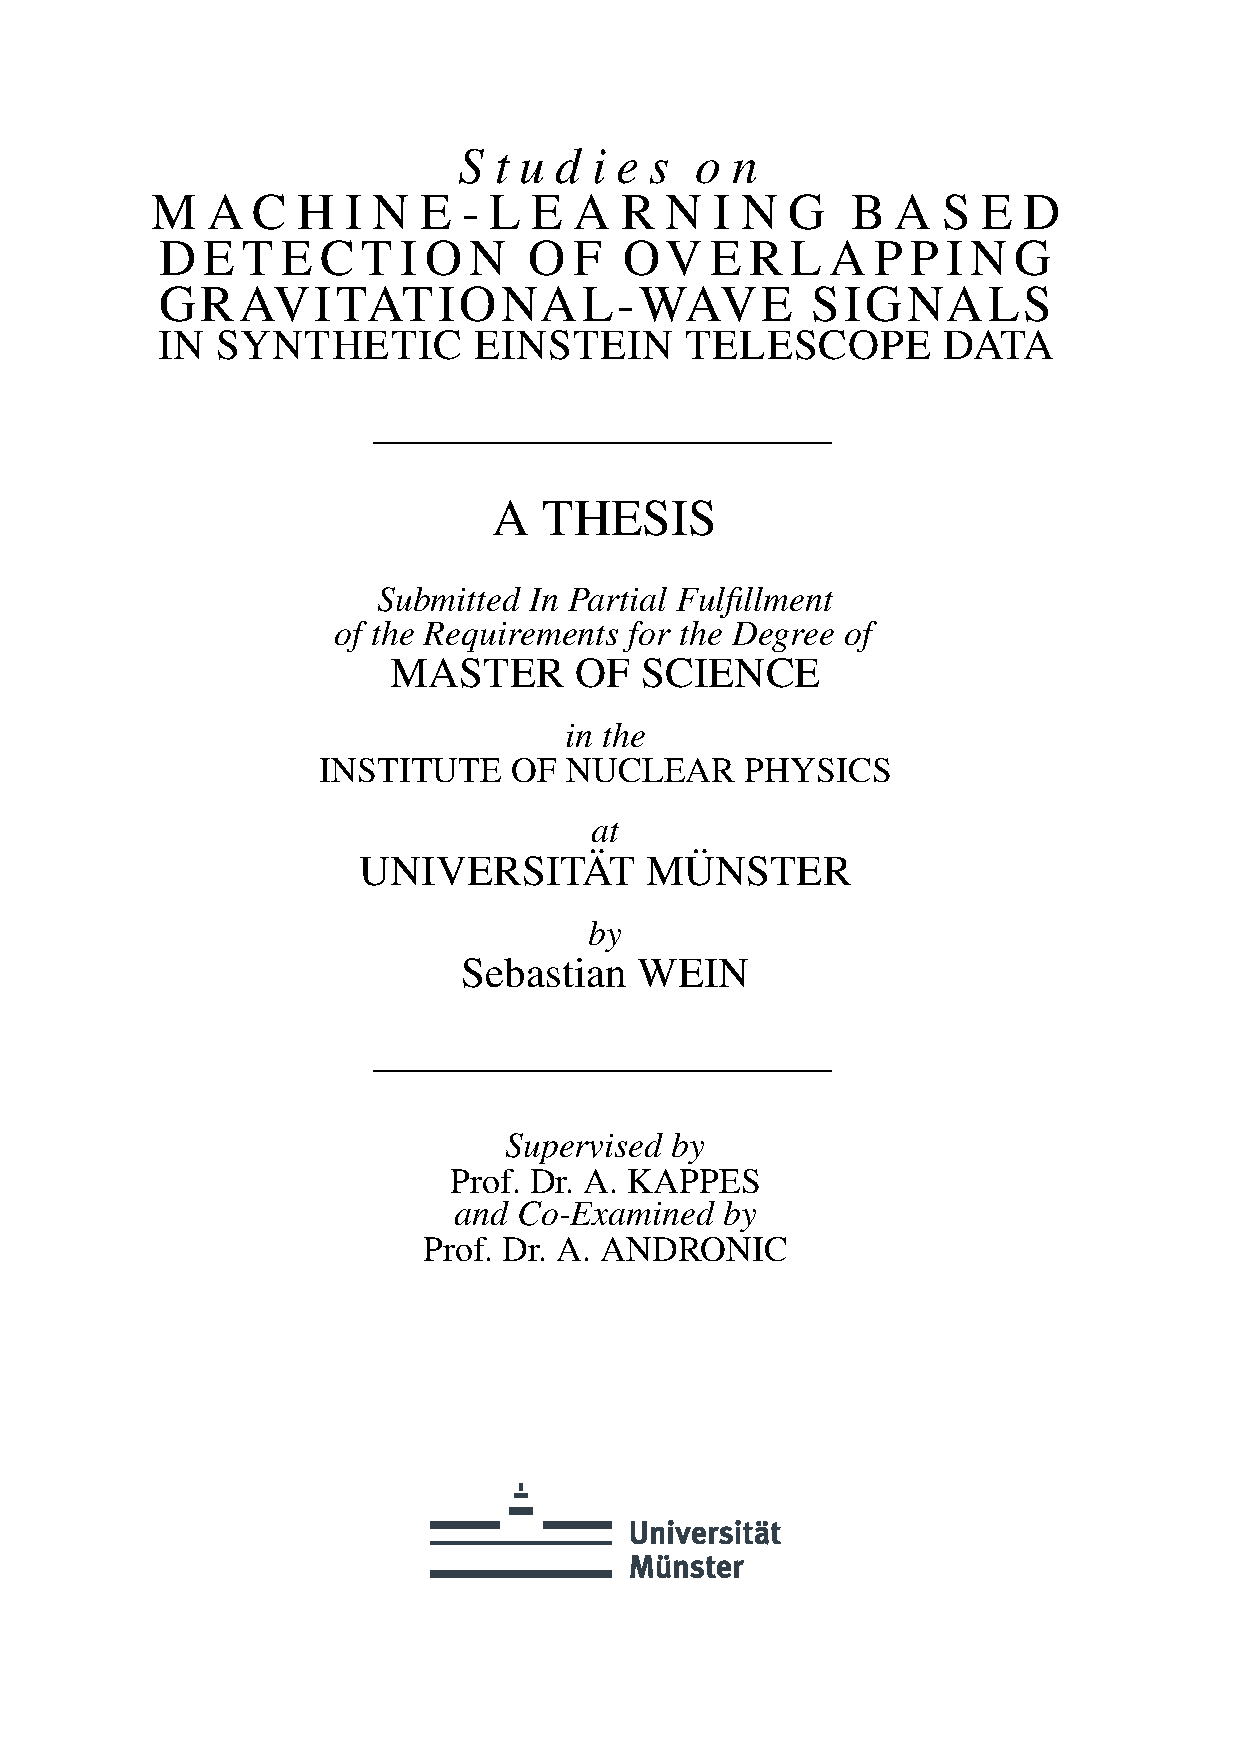
\includepdf{titlepage}

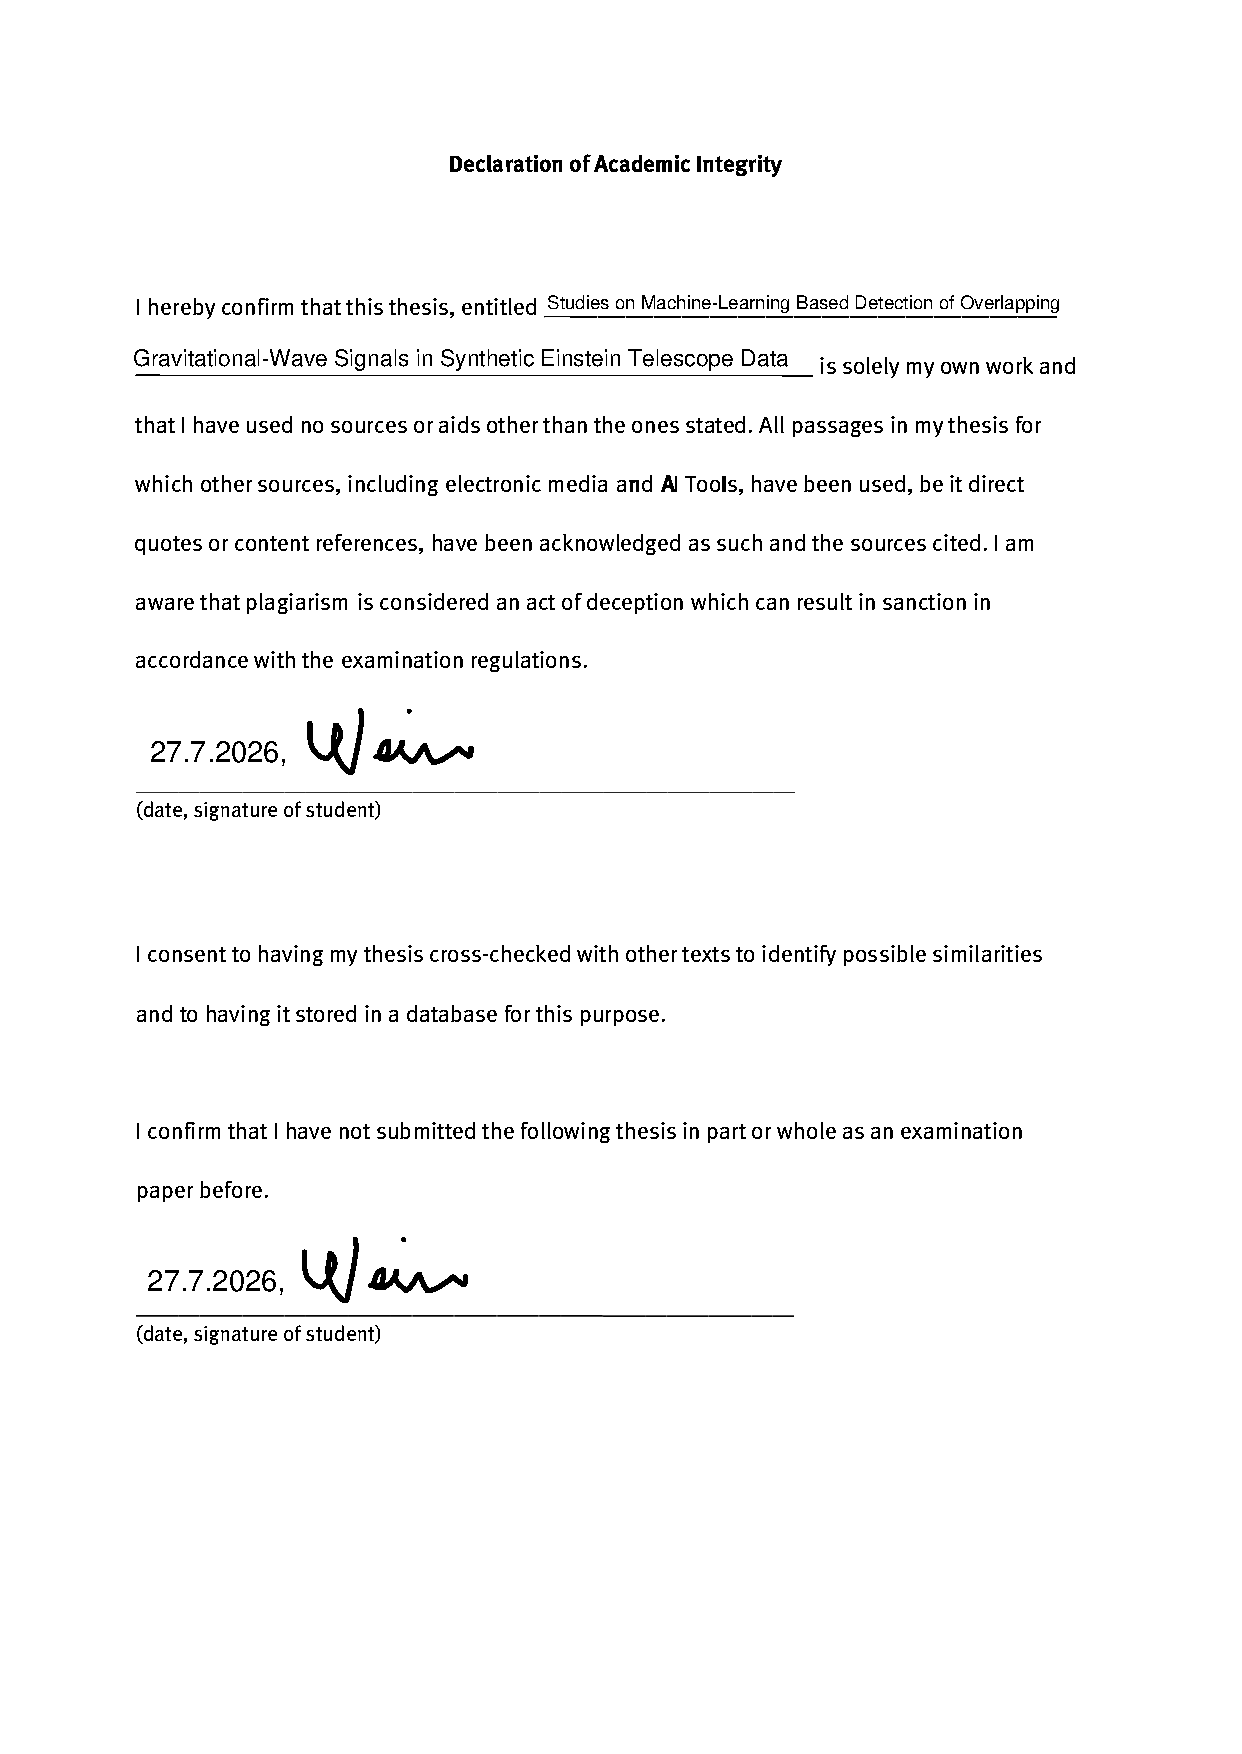
\includepdf[openright=true]{plagiatserklarung_eng_neu_signed}

\tableofcontents

\chapter{Introduction}
\setcounter{page}{1}
\pagenumbering{arabic}
\begingroup
% \boolfalse{citerequest}
% what are GWs
% very faint -> only massive astrophysical objects
% detection using laser interferometers
% main signal CBCs (maybe mention ligo and gw150914)

Gravitational waves (GWs) are small oscillating perturbations of the spacetime metric caused by accelerating masses.
Because they are so faint, only GW signals emitted by massive astrophysical objects have any chance of being detected. 
In particular, these are GWs emitted during the coalescence, \emph{i.e.}\ the inspiral and merger, of a system of two black holes or neutron stars. These types of systems are called \emph{compact binary coalescences} (CBCs) and give rise to a \enquote{chirp}-like GW signal, increasing in frequency and amplitude up until the merger of the two objects.

Large-scale laser interferometers allow for the detection of these GW signals. They are used at facilities such as LIGO~\cite{Abbott_2009, Aasi_2015}, where the first direct observation of gravitational waves was achieved in 2015 \cite{PhysRevLett.116.061102}. Currently there are a handful of such sites operating, forming the network of second-generation GW detectors.

As the current generation of detectors is reaching their design sensitivities and facility limits, a new third generation of detectors is being proposed.
One of these is the Einstein Telescope (ET) \cite{Punturo_2010, Hild_2011}, which will be based in Europe.
% \cite{abac2025scienceeinsteintelescope, Branchesi_2023}
ET aims for an improved design sensitivity compared to second-generation detectors, particularly in the low-frequency regime $\pazocal{O(\SI{1}{\hertz})}$.  
However, with this increase in sensitivity, new challenges for \emph{signal detection} arise. In this context, signal detection refers to the identification of GW signals in the detector data stream. 
The challenge is mostly the growing quantity of information in the data and the increased computational power needed to extract it. ET will detect more signals in total, and these signals will stay up to minutes or hours in the detector's sensitivity band. Combined, this leads to frequent signal time-overlap.

% up to now: matched filtering
% does not scale well for long overlapping signals

For second-generation data, GW searches rely on \emph{matched filtering} to produce event candidates \cite{PhysRevD.85.122006, Usman_2016}. 
However, this algorithm is known to not scale well in time and memory complexity when handling long and overlapping signals. This is especially problematic for \emph{low-latency} searches, which produce triggers for data monitoring and multi-messenger astronomy in real time. 	

Previously, the need for low-latency search algorithms has motivated the investigation of alternatives to matched filtering. Notably, \emph{machine-learning} has shown promising results while being far more computationally efficient \cite{George_2018, PhysRevD.100.063015}. The research focuses mostly on convolutional neural networks (CNNs) for detecting GW signals in second-generation detector conditions.
For ET-like data with overlapping signals, a different type of architecture has proven successful for GW parameter estimation instead \cite{Papalini_2025}. Namely, that is the Transformer~\cite{NIPS2017_3f5ee243} architecture, whose performance for GW detection is not well studied.

This work aims to implement machine-learning models to detect long-duration, overlapping CBC signals in ET conditions. Motivated by the results in \cite{Papalini_2025}, the performance of transformer-based architectures will be compared to more standard CNN approaches. 

The rest of this thesis is structured as follows: Ch.~\ref{sec:gravitational_waves} provides some theoretical background on GWs, and Ch.~\ref{sec:einstein_telescope} introduces ET.  Ch.~\ref{sec:matched_filtering} describes GW searches with matched filtering. After that follows an introduction to machine learning in Ch.~\ref{sec:machine_learning}, focusing on CNNs and the Transformer.
Training neural networks requires synthetic ET-like data, and Ch.~\ref{sec:data_simulation} will be a detailed description of the simulation of this data. 

The results are split in two parts.
Ch.~\ref{sec:long_duration} isolates the problem of processing the large inputs required to capture the long-duration signals that are expected for ET. Chs.~\ref{sec:heatmap} and \ref{sec:detr} deal with detecting multiple overlapping signals. Each time, two models are compared: one more closely resembling existing approaches and one being novel.
The thesis concludes with a summary of its findings and an outlook in Ch.~\ref{sec:conclusion}.

% focus on this work's contribution which is transformer based overlapping signal detection 
% real time detection compared to matched which is not 
% goal: low-latency CBC search with machine learning -> can be adapted to unmodelled signals as a bonus
\endgroup

\chapter{Gravitational Waves} 
\label{sec:gravitational_waves}
% \booltrue{citerequest}
The existence of gravitational waves is a direct consequence of Einstein's theory of general relativity (GR), which describes gravity in terms of the differential geometry of curved spacetime. The theory states that the presence of matter causes a curvature of spacetime and particles move along the shortest path in this curved space, along so-called \emph{geodesics}.
This chapter provides a brief introduction to general relativity and how gravitational waves emerge from this theory. It discusses their properties and astrophysical sources, focusing on compact binary systems since these are the only type of signals considered in this work. The sources for this chapter are \cite{10.1093/acprof:oso/9780198570745.001.0001} and to a lesser extent \cite{Carroll_2004}. 

\section{General Relativity}

%\begin{figure}
%	\centering
%	\makebox[\textwidth]{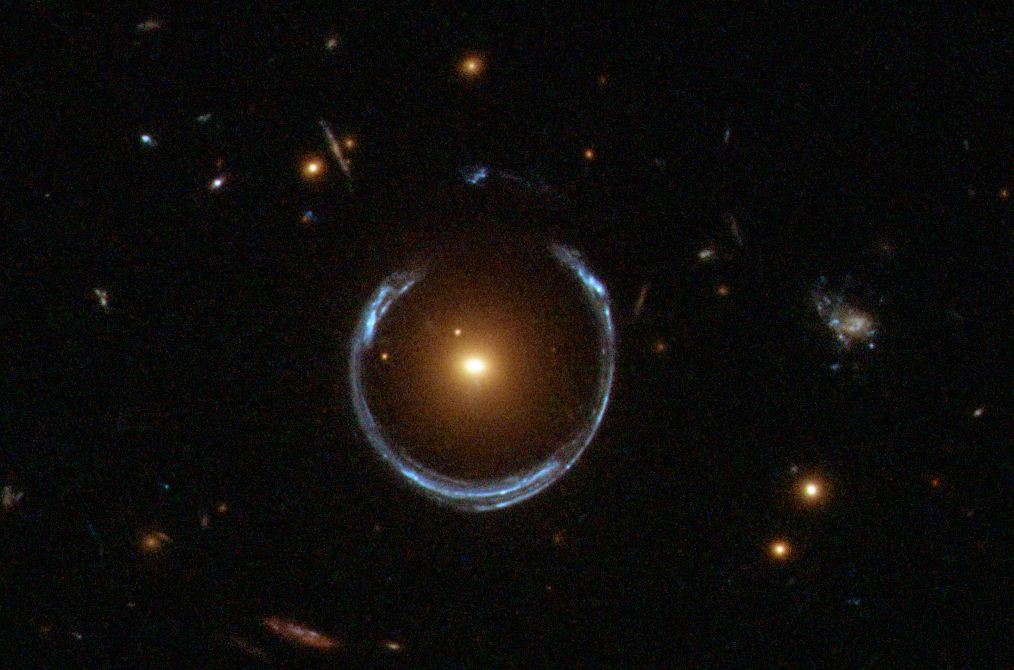
\includegraphics[width=5cm]{theory_of_gravitational_waves/images/A_Horseshoe_Einstein_Ring_from_Hubble}}
%	\caption{}
%	\label{fig:gravitational_waves:lensing}
%\end{figure}	

The theory of general relativity is based on the \emph{strong equivalence principle}, which states that there is no way to distinguish free-falling frames from one another by performing local experiments and that locally, \emph{special relativity} holds. This postulate alone gives rise to effects such as gravitational redshift or the bending of light near large masses. The equivalence principle then leads to a four-dimensional geometric description of spacetime, which is based on the metric tensor $g_{\mu\nu}$ whose indices denote the time and spatial axes, $t$, $x$, $y$ and $z$.
The metric tensor defines local distances in curved spacetime which are invariant under coordinate transformations through the differential line element,
\begin{equation}
	\label{eq:gravitational_waves:line_element}
	\mathrm{d}s^2 = g_{\mu\nu}\mathrm{d}x^\mu\mathrm{d}x^\nu
\end{equation}
with $x^\mu = (ct, \vec{r})$ where $c$ is the speed of light.
This is a generalization from the invariant quadratic form in special relativity, where
spacetime is flat. Then, the metric tensor is the \emph{Minkowski} metric $\eta_{\mu\nu} = \diag(-1, 1, 1, 1)$ and Eq.~\ref{eq:gravitational_waves:line_element} reads 
\begin{equation}
	\mathrm{d}s^2 = -c^2\mathrm{d}t^2 + \mathrm{d}x^2 + \mathrm{d}y^2 + \mathrm{d}z^2.
\end{equation}

The equations of motion for the metric $g_{\mu\nu}$ can be derived by defining the gravitational action, which depends on the metric itself and the matter content. Then, by requiring that the variation of this action with respect to the metric be zero, one arrives at the \emph{Einstein equations},
\begin{equation}
	\label{eq:gravitational_waves:einstein_eqs}
	R_{\mu\nu} - \frac{1}{2}Rg_{\mu\nu} = \frac{8\pi G}{c^4}T_{\mu\nu}.
\end{equation}
These equate the \emph{energy-momentum tensor} $T_{\mu\nu}$ with the \emph{Einstein tensor} $G_{\mu\nu} = R_{\mu\nu} - Rg_{\mu\nu}/2$ on the left-hand side up to some constant, where $G$ is Newton's constant. The energy-momentum tensor describes the matter and energy content and the Einstein tensor expresses the resulting spacetime curvature. The latter is constructed from the metric $g_{\mu\nu}$ as well as the \emph{Ricci tensor} $R_{\mu\nu}$ and the \emph{Ricci scalar} $R$, both of which also depend on the metric through various partial derivatives and index contractions. 

Without any forces acting, particle trajectories will follow geodesics of this curved spacetime.
Knowing the spacetime curvature, these can be calculated using the \emph{geodesic equation},
\begin{equation}
	\label{eq:gravitational_waves:geodesic_eq}
	\frac{\mathrm{d}^2x^\lambda}{\mathrm{d}\tau^2} 
	+ \Gamma^\lambda_{\mu\nu}\,
	\frac{\mathrm{d}x^\mu}{\mathrm{d}\tau}\,
	\frac{\mathrm{d}x^\nu}{\mathrm{d}\tau}
	= 0
\end{equation}
where $\tau$ is the particle's proper time and $\Gamma^\lambda_{\mu\nu}$ denote the \emph{Christoffel symbols} which depend on the curvature. 
% what is proper time? the time the particle measures along its trajectory that is in its reference frame which is at rest ds = c dtau

It can be seen that GWs naturally emerge from GR when working in \emph{linearized theory}: The GW's effect on spacetime is thought of as a \enquote{small} perturbation $h_{\mu\nu}$ of flat spacetime. Then, spacetime can be expanded as
\begin{equation}
	\label{eq:gravitational_waves:linearized_theory}
	g_{\mu\nu} = \eta_{\mu\nu} + h_{\mu\nu} \quad\text{with $|h_{\mu\nu}|\ll1$},
\end{equation}
and any terms of higher order than $\pazocal{O}(h_{\mu\nu})$ are neglected in following calculations. Further simplifications can be made by noting that
GR is invariant under \emph{all possible} coordinate transformations. This corresponds to large number of degrees of freedom, \emph{i.e.}, a large \emph{gauge symmetry}. 
Imposing linearized theory breaks that invariance, but still a residual gauge symmetry remains. 
% this is sloppy and wrong maybe?
Thus, the \emph{Lorenz gauge} can be chosen, $\partial^\mu\bar{h}_{\mu\nu} = 0$. Then the Einstein equations (Eq.~\ref{eq:gravitational_waves:einstein_eqs}) simply reduce to wave equations,
\begin{equation}
	\label{eq:gravitational_waves:wave_eq}
	\square\,\bar{h}_{\mu\nu} = -\frac{16\pi G}{c^4}\,T_{\mu\nu}
\end{equation}
with the d'Alembertian $\square=\partial_\mu\partial^\mu=-\partial_t^2/c^2 + \nabla^2$.\footnote{Indices are raised and lowered using the Minkowski metric in linearized theory.}
Here, $\bar{h}_{\mu\nu}$ denotes the \emph{trace-reversed} perturbation, which is defined as
\begin{equation}
	\bar{h}_{\mu\nu} = h_{\mu\nu}-\frac{1}{2}\eta_{\mu\nu}h,
\end{equation}
where $h = \eta^{\mu\nu}h_{\mu\nu}$ is the original perturbation's trace. The trace-reversed perturbation gets its name from the fact that its trace $\bar{h} = \eta^{\mu\nu}\bar{h}_{\mu\nu} = -h$. Obviously, the original perturbation can be reconstructed from the trace-reversed one, so no information is lost. 
Eq.~\ref{eq:gravitational_waves:wave_eq} shows that GWs obey an inhomogeneous wave equation with the matter content $T_{\mu\nu}$ as its source. 

\section{Properties in Vacuum}

To study the propagation of GWs and their influence on nearby particles (also called test masses in this context) it makes sense to consider the case far away from the sources that produce them. This is called the \emph{vacuum case}, where $T_{\mu\nu} = 0$.
The Einstein equations (Eq.~\ref{eq:gravitational_waves:wave_eq}) now read,
\begin{equation}
	\label{eq:gravitational_waves:homogeneous_wave_eq}
	\square\,\bar{h}_{\mu\nu} = 0.
\end{equation}
These equations have plane-wave solutions, 
\begin{equation}
	\bar{h}_{\mu\nu} = A_{\mu\nu}\,\e^{ik_\rho x^\rho}
\end{equation}
with a wave-vector $k^\mu = (\omega/c, \vec{k})$ and some constant amplitude $A_{\mu\nu}$. This introduces complex numbers, and only the real part is considered at the end of calculations. For the plane-wave solutions, the Einstein equations (Eq.~\ref{eq:gravitational_waves:homogeneous_wave_eq}) imply that $k_\mu k^\mu = 0$, which loosely translates to the fact that GWs propagate at the speed of light. The Lorenz gauge condition yields $A^{\mu\nu}k_\mu=0$, \emph{i.e.}, the amplitude and wave-vector are orthogonal.

Now for reasons that will not be laid out here, the vacuum case allows for the introduction of the \emph{transverse-traceless} gauge with
\begin{equation}
	h^{0\mu} = 0 \quad \text{and} \quad h^i_{\phantom{i}i} = 0,
\end{equation}
where Latin indices, such as $i,j,k$, denote spatial components only. For further information, consult \cite{10.1093/acprof:oso/9780198570745.001.0001}. In this gauge the trace $h$ vanishes and thus $\bar{h}_{\mu\nu} = h_{\mu\nu}$. The Lorenz condition then reads $A^{ij}k_j=0$: GWs are transverse, meaning they perturb the metric orthogonal to their propagation direction.

\begin{figure}
	\centering
	\makebox[\textwidth]{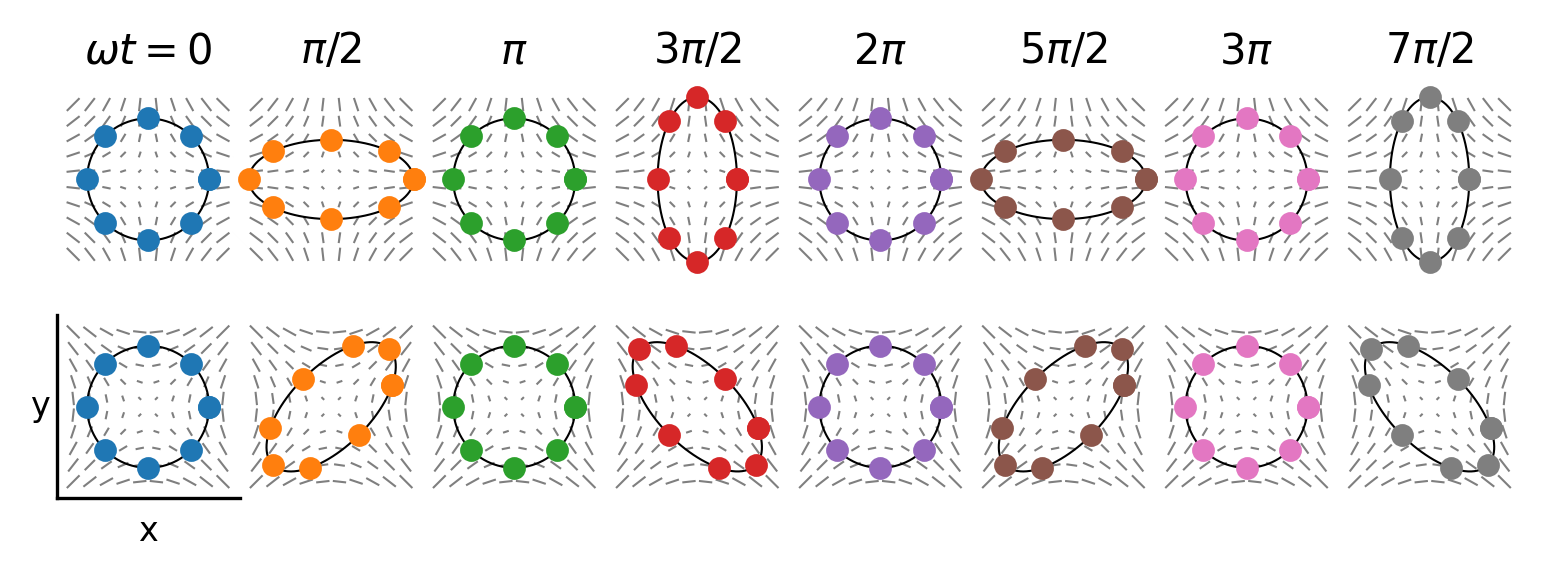
\includegraphics[width=16cm]{theory_of_gravitational_waves/images/test_masses/polarization_trajectories}}
	\caption{The effect of a passing GW on a ring of test masses on the transverse plane. The top row shows a purely plus-polarized GW, and the bottom row a cross-polarized one.}
	\label{fig:gravitational_waves:polarization}
\end{figure}

To illustrate their effect on test masses, one can arbitrarily choose a GW to propagate along the z-axis, $\vec{k}=(0,0,\omega/c)$. Enforcing the gauge conditions, only two components of the amplitude remain and the GW perturbation takes the following form:
\begin{equation}
	h_{\mu\nu} = \begin{pmatrix}
		0 & 0 & 0 & 0 \\
		0 & A_+ & A_\times & 0 \\
		0 & A_\times & -A_+ & 0 \\
		0 & 0 & 0 & 0
	\end{pmatrix}_{\mu\nu} \e^{i\omega(t-\frac{z}{c})} = h_+e_{\mu\nu}^+ + h_\times e_{\mu\nu}^\times
\end{equation}
with $h_+ = A_+\exp i\omega(t-z/c)$ and $h_\times = A_\times\exp i\omega(t-z/c)$.
The result is split along two linearly independent polarizations, labeled \emph{plus} (\text{$+$}) and \emph{cross} (\text{$\times$}). Each is described by a polarization tensor, $e_{\mu\nu}^+$ and $e_{\mu\nu}^\times$, which are orthogonal, $e_{\mu\nu}^+e^\times{}^{\mu\nu} = 0$. The plus and cross polarization states get their names from their effect on nearby test masses.

The trajectories of nearby particles with separation vectors $S^\mu$ follow from the geodesic equation (\ref{eq:gravitational_waves:geodesic_eq}). It can be seen that the test masses are only perturbed perpendicular to the GW's propagation direction in the x--y plane. In particular, solving for a purely plus-polarized wave, $h_\times=0$, yields
\begin{equation}
	\label{eq:gravitational_waves:plus_polarization}
	\begin{aligned}
		S^1 &= S^1(0) + \frac{h_+}{2}\,S^1(0), \quad
		S^2 &= S^2(0) - \frac{h_+}{2}\,S^2(0).
	\end{aligned}
\end{equation}
Thus, particles initially separated on the x-axis will oscillate in that same direction; likewise for particles on the y-axis but with a phase shift of \SI{180}{\degree}. Considering a ring of test particles around the origin, one can see that they oscillate in a plus-shaped manner.
Now, in the case that the GW is purely cross-polarized, $h_+=0$ and $h_\times\neq0$, the solution is instead given by
\begin{equation}
\label{eq:gravitational_waves:cross_polarization}
\begin{aligned}
	S^1 &= S^1(0) + \frac{h_\times}{2}\,S^2(0), \quad
	S^2 &= S^2(0) - \frac{h_\times}{2}\,S^1(0),
\end{aligned}
\end{equation}
and a ring of test masses will oscillate cross-wise.
The effect of these two polarization states can be seen plotted in Fig.~\ref{fig:gravitational_waves:polarization}.

\section{Production}
\label{sec:gravitational_waves:production}

Having studied their properties in the vacuum case, one can now take one step back and consider the production of GWs. This means considering $T_{\mu\nu} \neq 0$ (where now only the Lorenz gauge and \emph{not} the transverse-traceless gauge can be chosen), in which case the Einstein equations take the form of an inhomogeneous wave equation again, $\square\,\bar{h}_{\mu\nu} = -(16\pi G/c^4)\,T_{\mu\nu}$ (see Eq.~\ref{eq:gravitational_waves:wave_eq}). The solutions to this equation are known:
\begin{equation}
	\bar{h}_{\mu\nu} = \frac{4G}{c^4} 
	\int\mathrm{d}^3\vec{r}'\, 
	\frac{T_{\mu\nu}\bigl(t-\frac{|\vec{r}-\vec{r}'|}{c}, \vec{r}'\bigr)}
	{|\vec{r}-\vec{r}'|}.
\end{equation}
That is, the GW perturbation observed at position $(t, \vec{r})$ is caused by the sum of all sources $T_{\mu\nu}$ evaluated at time $t_\text{ret} = t-|\vec{r}-\vec{r}'|/c$, the \emph{retarded time}. (If a source at $\vec{r}'$ emits a signal at time $t_\text{ret}$ it will reach the observer position $\vec{r}$ at time $t$.) Making the assumption that the source volume is \enquote{small} and that it is far away from the observer allows approximating the distance between the two as $|\vec{r}-\vec{r}'| \approx |\vec{r}| = r$.
Thus, 
\begin{equation}
	\bar{h}_{\mu\nu} = \frac{4G}{c^4r} \int\mathrm{d}^3\vec{r}'\, 
	T_{\mu\nu}(t_\text{ret}, \vec{r}'),
\end{equation}
where the approximation is made that the source slowly moving such that $t_\text{ret} = t-r/c$. % not sure if this is correct, see Durandar
Furthermore, properties of the stress-energy tensor turn out to prove that
\begin{equation}
	\int\mathrm{d}^3\vec{r}\,T_{ij}(t, \vec{r}) 
	= \frac{1}{2}\frac{\partial_t^2}{c^2}\int\mathrm{d}^3\vec{r}\, r_ir_jT_{00}(t, \vec{r}) 
	= \frac{1}{2}\partial_t^2 Q_{ij}(t),
\end{equation}
where $Q_{ij}$ is the \emph{quadrupole moment tensor}, defined as
\begin{equation}
	Q_{ij}(t) = \frac{1}{c^2}\int\mathrm{d}^3\vec{r}\ r_ir_jT_{00}(t, \vec{r}).
\end{equation}
Putting all together, the spatial components of the trace-reversed perturbation are given by
\begin{equation}
	\label{eq:gravitational_waves:quadrupole_formula}
	\bar{h}_{ij} = \frac{2G}{c^4}\frac{1}{r}\partial_t^2Q_{ij}(t_\text{ret}),
\end{equation}
and the remaining four components $\bar{h}^{0\mu}$ can be found by demanding the Lorenz gauge condition be satisfied. 
% TODO: this kind of ugly because the energy momentum tensor just falls from heaven like if you dont wanna do the whole derivation dont bother and dont half ass it like you did here

% TODO: give some intuition
Eq.~\ref{eq:gravitational_waves:quadrupole_formula} is known as the \emph{quadrupole formula}.
It implies two things: that GWs are emitted by systems with a time-varying quadrupole moment (to leading order) and that their amplitude decays inversely with the distance from the source. Thus, static sources do not radiate and neither do spherically symmetric sources since their mass quadrupole moment is zero\footnote{The quadrupole moment is only non-vanishing for mass distributions with a non-zero $l=2$ spherical harmonic contribution. Thus spherically symmetric systems ($l=0$) do not emit GWs, while orbiting binary systems ($l=2$) do radiate. See App.~\ref{app:quadrupole}}. Note that the prefactor $G/c^4$ is of order \SI{E-45}{} in SI units, so GW perturbations are typically very small. The most promising sources for GW production will be massive objects with large kinetic energy. Such sources include rapidly spinning neutron stars with some mass asymmetry or compact binary systems of black holes (BBH) or neutron stars (BNS). 

\section{Compact Binary Coalescences}

This latter case of radiating compact binary systems is called \emph{compact binary coalescences} (CBCs). These are systems of two masses in compact orbit. The system loses energy in the form of GW emission, thus the orbital radius will decrease until the two objects merge. This is the only type of GW signal detected so far, which is mostly emitted by black hole binaries. 

Using the quadrupole formula, the approximate form of the emitted GW can be calculated. (This closely follows \cite{10.1093/acprof:oso/9780198570745.001.0001}.) To this end, the orbital motion is assumed to be Newtonian and the bodies treated as point-particles. The masses will be denoted $m_1$ and $m_2$ and their positions $\vec{r}_1$ and $\vec{r}_2$. In the center-of-mass frame, the system reduces to a one-body problem with effective mass $\mu = m_1m_2/M$ and relative position $\vec{\rho} = \vec{r}_2 - \vec{r}_1$, where $M=m_1+m_2$ is the total mass. The bodies' motion is governed by $\partial_t^2\vec{\rho} = -(GM/R^3)\,\vec{\rho}$ with $R=|\vec{\rho}|$. In the simplest case, the orbit will be circular with angular frequency $\omega = \surd GM/R^3$. Choosing the x--y plane as the orbital plane, this means
\begin{equation}
	\label{eq:gravitational_waves:cbc_pos}
	\vec{\rho} = R\,\begin{pmatrix}
		\cos(\omega t + \frac{\pi}{2}) &
		\sin(\omega t + \frac{\pi}{2}) &
		0
	\end{pmatrix}^\intercal.
\end{equation}
Then, $T_{00}(t, \vec{r}) = c^2\mu\delta(\vec{r}-\vec{\rho})$, and after projecting the quadrupole moment tensor to the transverse-traceless gauge, the quadrupole formula yields
\begin{align}
\label{eq:gravitational_waves:cbc_waveform}
\begin{split}
	h_+(t) &= \frac{4}{r}
	\left(\frac{G\pazocal{M}}{c^2}\right)^\frac{5}{3}
	\left(\frac{\omega}{c}\right)^\frac{2}{3}
	\frac{1+\cos^2\theta}{2}\,\cos(2\omega t_\text{ret} + 2\phi), \\
	h_\times(t) &= \frac{4}{r}
	\left(\frac{G\pazocal{M}}{c^2}\right)^\frac{5}{3}
	\left(\frac{\omega}{c}\right)^\frac{2}{3}
	\cos\theta\sin(2\omega t_\text{ret} + 2\phi),
\end{split}
\end{align}
where $\theta$ and $\phi$ are the polar and azimuth angles respectively, and the \emph{chirp mass} is introduced as $\pazocal{M} = \mu^{3/5}(m_1+m_2)^{2/5}$. Note that the resulting GW signal oscillates with a frequency  $f$ that is twice the orbital frequency $\nu=\omega/2\pi$, that is, $f = 2\nu = \omega/\pi$.

% TODO: 3d plot?
\begin{wrapfigure}[16]{R}{4cm}
    % \hspace*{1cm}
	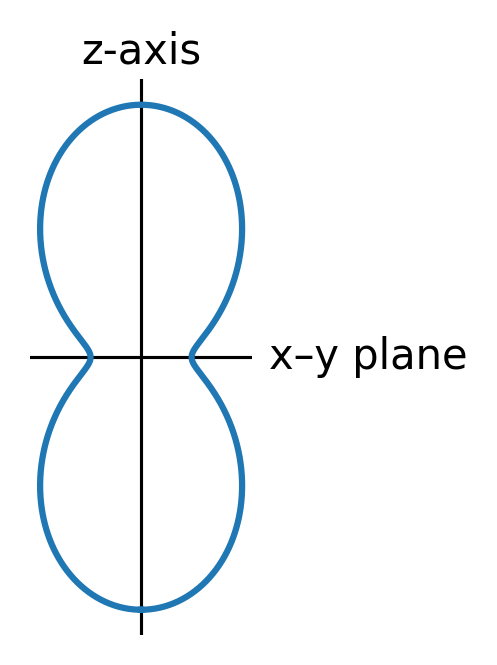
\includegraphics[width=4cm]{theory_of_gravitational_waves/images/cbc_quadrupole/radiation_pattern}
	\caption{Radiation pattern of a CBC system in the x--y plane visualized by plotting $g(\theta)\,(\cos\theta,\,\sin\theta)$} 
	\label{fig:gravitational_waves:radiation_pattern}
	% \vspace{-10pt}
\end{wrapfigure}

%\begin{equation}
%	P = -\frac{32}{5}\frac{c^5}{G}\left(\frac{G\pazocal{M}\pi f}{c^3}\right)^\frac{10}{3}
%\end{equation}
It can be shown that the radiated power per unit solid angle takes on the following form: 
\begin{equation}
	\frac{\mathrm{d}P}{\mathrm{d}\Omega} = \frac{2}{\pi}\frac{c^5}{G}\left(\frac{G\pazocal{M} \omega}{c^3}\right)^\frac{10}{3}g(\theta)
\end{equation}
with an angular distribution $g(\theta) = (1+\cos^2\theta)^2/4 + \cos^2\theta$.
(For further information consult \cite{10.1093/acprof:oso/9780198570745.001.0001}.)
This reveals that the radiated power scales with the orbital angular frequency $\omega^{10/3}$ and that most of that power is radiated along the z-axis, \emph{i.e.}\ perpendicular to the orbital plane (see Fig.~\ref{fig:gravitational_waves:radiation_pattern}). Now, the dependence on the frequency creates this feedback loop where the system continuously loses energy, which in turn decreases the orbital radius and increases the frequency leading to higher energy loss. This process gives rise to the characteristic chirp-like signal that is associated with CBCs, where up until the merger, the GW frequency and amplitude increase.

\begin{figure}
	\centering
	\makebox[\textwidth]{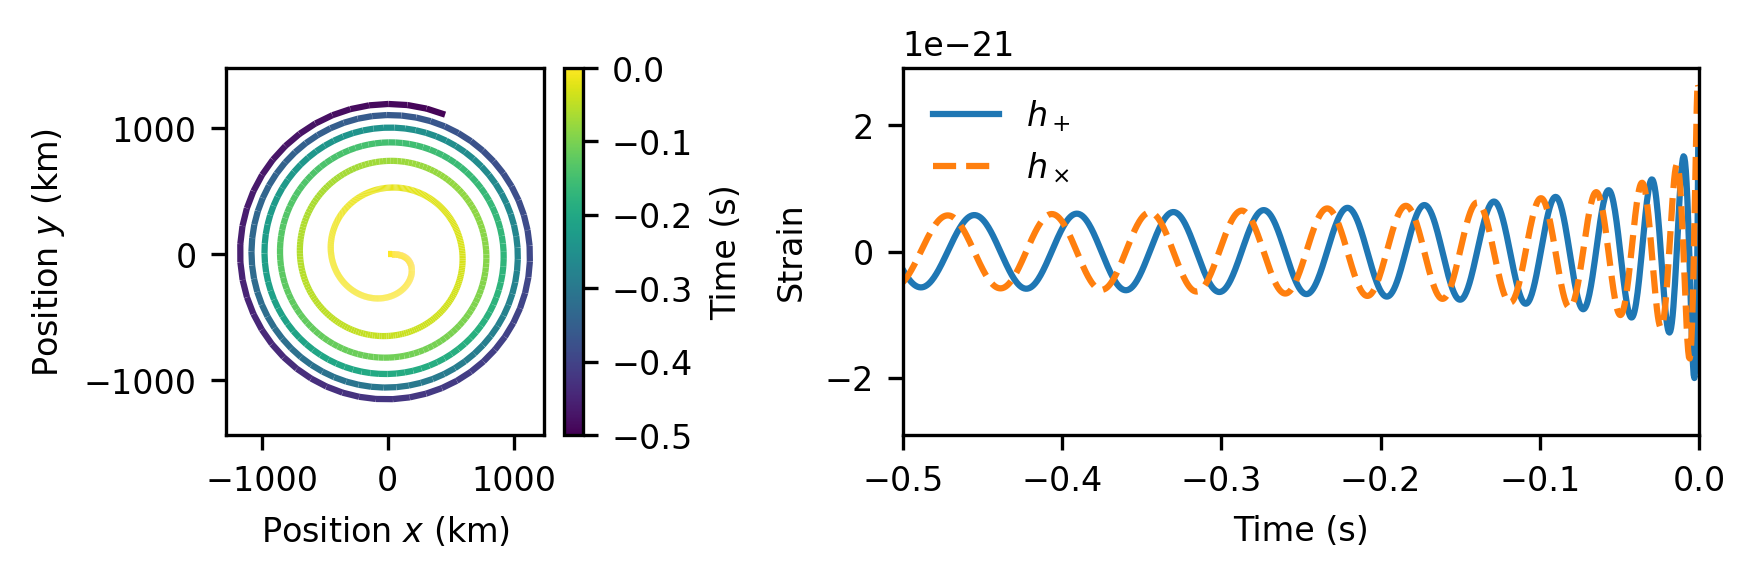
\includegraphics[width=15cm]{theory_of_gravitational_waves/images/coalescences/waveform}}
	\caption{Evolution of a CBC system. Trajectory of the reduced mass in the orbital plane in the center-of-mass frame on the left. The two polarizations of the emitted GW on the right.}
	\label{fig:gravitational_waves:waveform}
\end{figure}	
The evolution of $\omega(t)$ can be calculated by considering that the total energy of this system is $E = -Gm_1m_2/2R$. Equating $P$ and $-\mathrm{d}E/\mathrm{d}t$ results in a differential equation for $\omega$. Solving with respect to $\tau = t_\text{coa} - t$, the time to coalesce, yields
\begin{equation}
	\label{eq:gravitational_waves:cbc_freq}
	\omega(\tau) = \left(\frac{c^3}{G\pazocal{M}}\right)^\frac{5}{8}
	\left(\frac{5}{256}\frac{1}{\tau}\right)^\frac{3}{8}.
\end{equation}
With this result, the one-body motion in the center-of-mass frame can be obtained via Eq.~\ref{eq:gravitational_waves:cbc_pos} as well as the resulting GW waveform from Eq.~\ref{eq:gravitational_waves:cbc_waveform}. The dynamics of two inspiraling masses, \SI{40}{\solarmass} and \SI{30}{\solarmass}, and the emitted GW signal as measured at a distance of $r=\SI{500}{\mega\parsec}$ are plotted in Fig.~\ref{fig:gravitational_waves:waveform}. It can be seen in the last \SI{0.5}{\second}, the objects are very compact being separated by  $\pazocal{O}(\SI{100}{\kilo\meter})$. The corresponding signal is chirp-like and of order $\pazocal{O}(\SI{E-21})$, so very faint despite the large masses.

Observe that formally, the frequency diverges at the time of coalescence (Eq.~\ref{eq:gravitational_waves:cbc_freq}), which is of course unphysical. This divergence stems from the fact that the two objects get arbitrarily close. Realistically, the innermost stable orbit would be $r_\text{ISCO} = 6GM/c^2$, which corresponds to an angular orbital frequency of $\omega_\text{ISCO} = c^3/6\sqrt{6} GM$. This can be related to the emitted GW signal frequency as
\begin{equation}
	\label{eq:theory_of_gravitational_waves:max_freq_approx}
	f_\text{max} = \frac{\omega_\text{ISCO}}{\pi} 
	\approx \SI{4.4}{\kilo\hertz}\,\frac{\SI{1}{\solarmass}}{M}.
\end{equation}
For black hole binaries with masses $\pazocal{O}(\SI{10}{\solarmass})$ this means maximum frequencies of $\pazocal{O}(\SI{100}{\hertz})$ while neutron star binaries have masses $\approx\SI{1}{\solarmass}$ resulting in frequencies up to $\approx\SI{2000}{\hertz}$.


\chapter{The Einstein Telescope}
\label{sec:einstein_telescope}
The use of laser interferometers allows for the detection of gravitational waves at sites such as LIGO~\cite{Abbott_2009, Aasi_2015}, Virgo~\cite{Acernese_2008, Acernese_2014} and KAGRA~\cite{10.1093/ptep/ptx180}. These form the current second generation of GW observatories, which have opened the field of gravitational wave (GW) astronomy. The second-generation detectors are, however, approaching their design sensitivities, with future upgrades reaching the facility limits. As many science cases require an improvement in sensitivity by roughly one order of magnitude, a new third generation of detectors is being proposed. One of these is the Einstein Telescope (ET) \cite{Punturo_2010, Hild_2011}, which will be based in Europe. 
This chapter introduces ET, outlining the detection principle, its conceptual design and scientific goals.

\section{Interferometric Detection}

%  TODO: citation, also better figure maybe
\begin{figure}
	\centering
	\makebox[\textwidth]{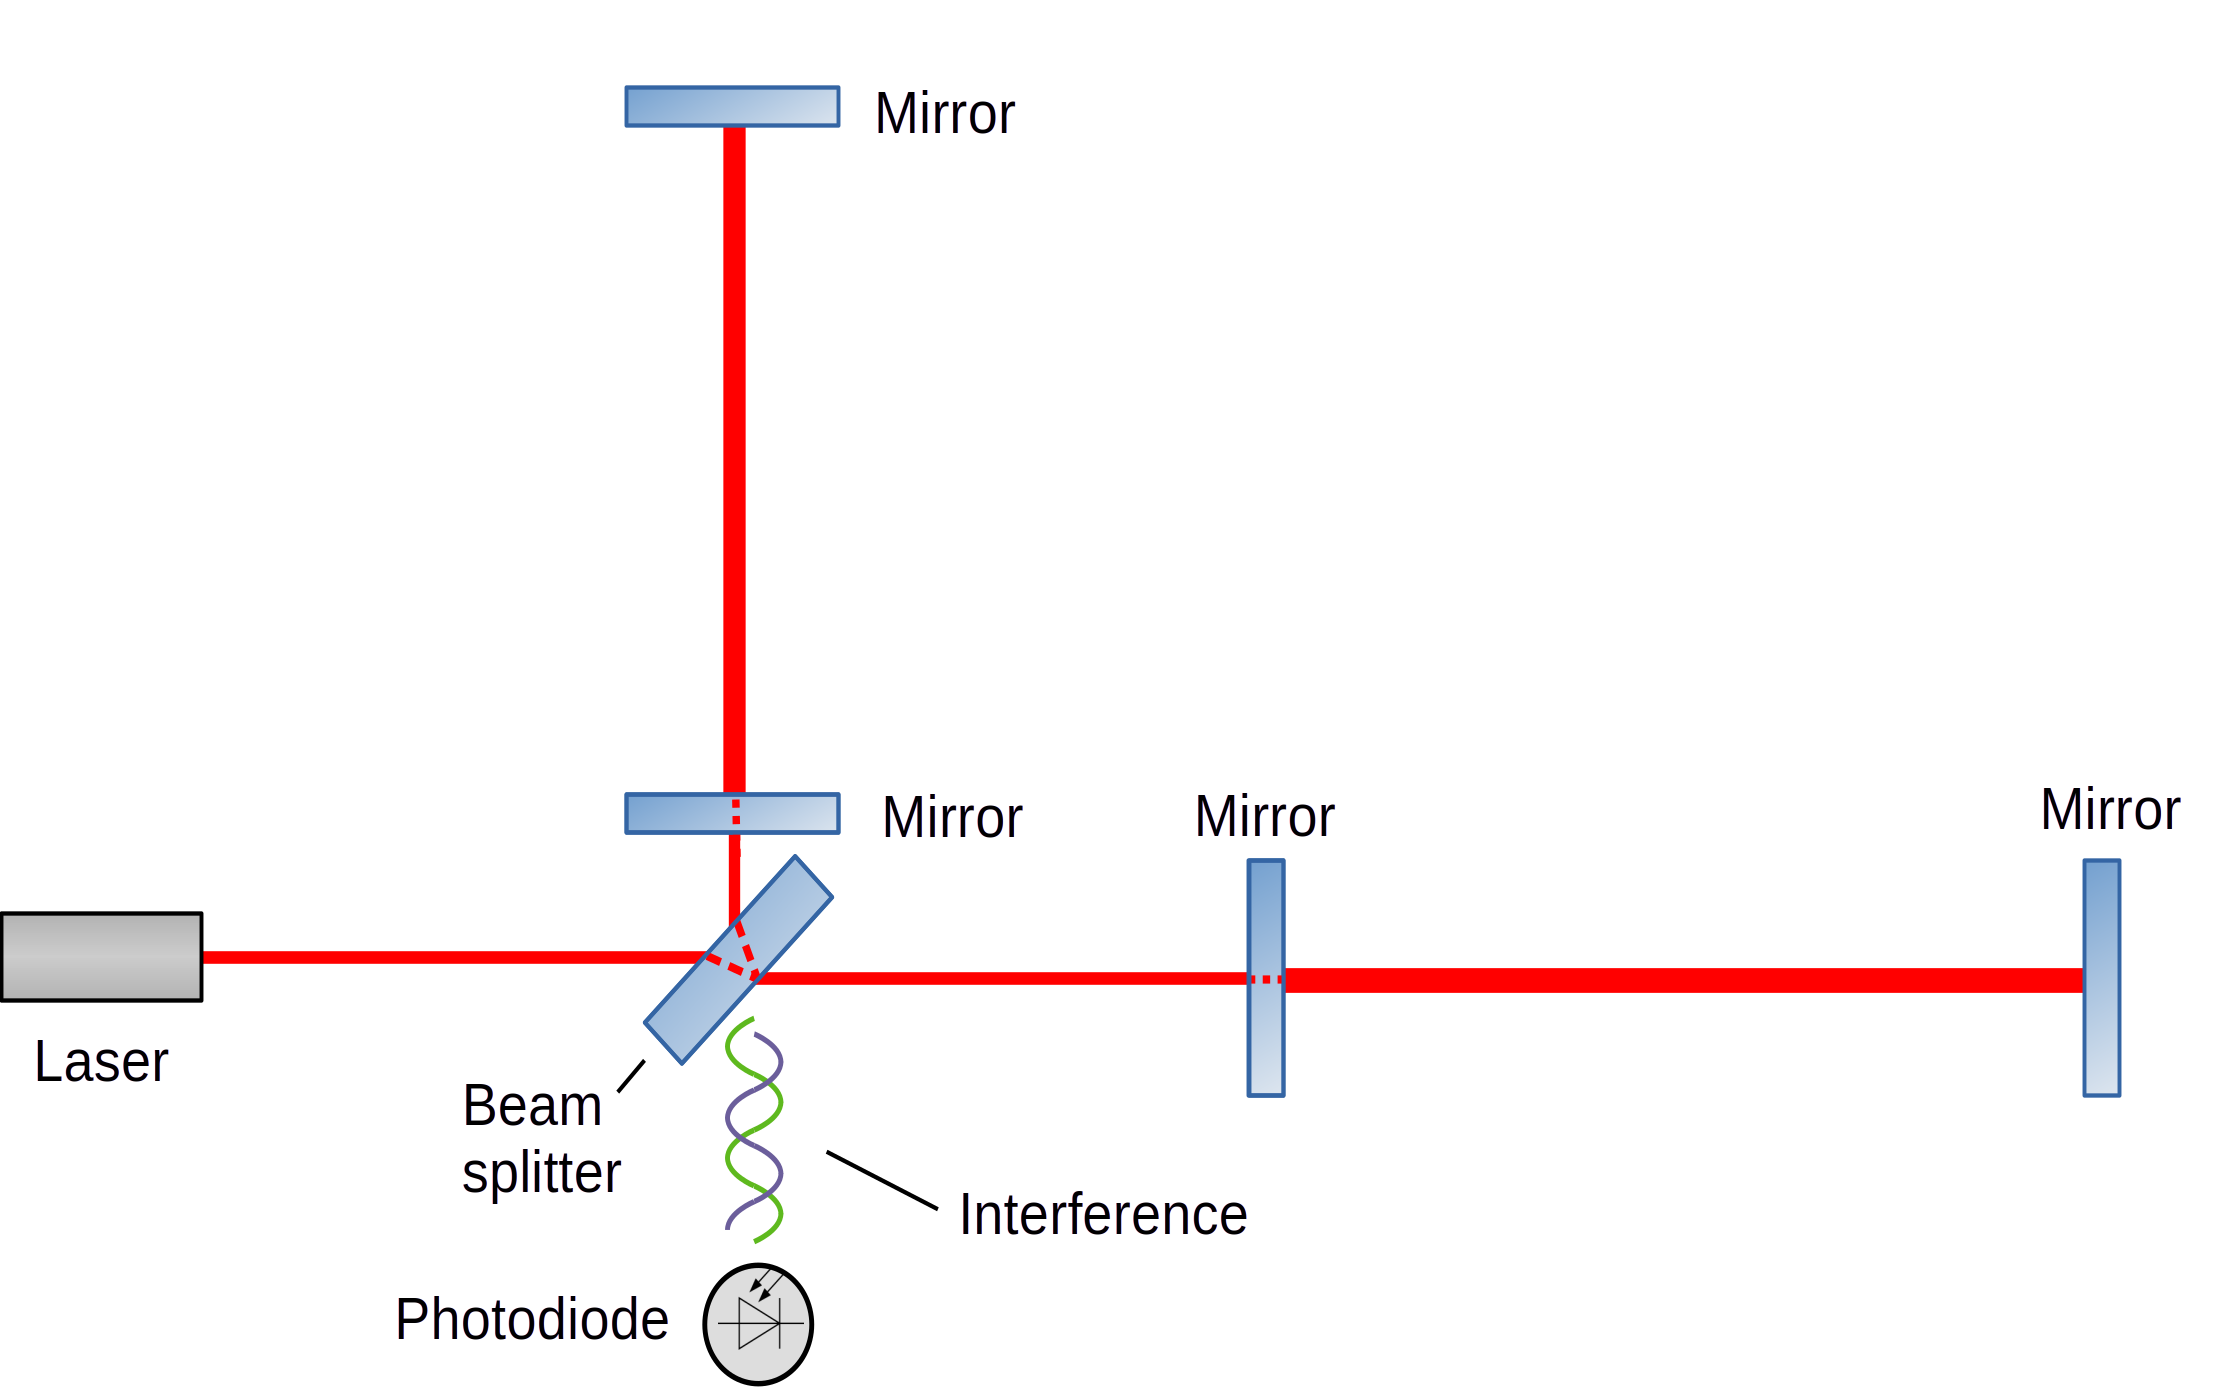
\includegraphics[width=14cm]{the_einstein_telescope/images/michelson/michelson}}
	\caption{Michelson laser-interferometer schematic, not drawn to scale. Usually, both arms will be of equal length. The extra mirrors near the beam splitter form power-enhancing \emph{Fabry-Perot cavities}.}
	\label{fig:einstein_telescope:michelson}
\end{figure}	

Ch.~\ref{sec:gravitational_waves:production} showed that the GW perturbations as measured on Earth are incredibly tiny, with amplitudes of $h \lesssim \SI{E-21}{}$, posing a significant challenge for direct detection. GWs are measured directly by observing their effect on test masses. From Eqs.~\ref{eq:gravitational_waves:plus_polarization} and \ref{eq:gravitational_waves:cross_polarization}, it is clear that a passing GW will cause displacement of the same order of magnitude as the perturbation $h$. This effect can be exploited using a \emph{Michelson laser interferometer} with its mirrors serving as the test masses. 

In the simplest case, this instrument consists of one laser, a beam splitter, two mirrors and a photo diode. The laser is directed towards the partially reflective beam splitter. The photons are sent down the two interferometer arms and reflected by mirrors at each end. The two beams travel back to the beam splitter where they are redirected to the photodiode measuring the resulting interference. 
A schematic is shown in Fig.~\ref{fig:einstein_telescope:michelson}.
The instrument is calibrated such that, in the absence of a GW, the beams interfere destructively at the photodiode. This is called \emph{dark fringe operation}.

This setup is enhanced by the inclusion of extra mirrors forming so-called \emph{Fabry-Perot cavities} with those mirrors at the end of each arm (see Fig.~\ref{fig:einstein_telescope:michelson}). The cavities increase the effective arm length as photons bounce back and forth a few hundred times before reaching the beam splitter again.

Now, suppose a purely plus polarized GW passes along the z-direction, 
and interferometer's arms lie on the x-axis and the y-axis. If the arms are of length $L$, the GW will cause length changes of  
$\Delta L_x = h_+L/2$ and $\Delta L_y = -h_+L/2$
respectively (see Eq.~\ref{eq:gravitational_waves:plus_polarization}). This leads to a path difference 
\begin{equation}
	\label{eq:einstein_telescope:path_difference}
	\Delta L = \Delta L_x - \Delta L_y = h_+L,	
\end{equation} 
which results in a phase difference of $\Delta \phi = (2\pi/\lambda) \Delta L$ with the laser wavelength $\lambda$. For arms of $\pazocal{O}(\SI{1}{\kilo\meter})$ the path differences will be $\pazocal{O}(\SI{E-18}{\meter})$, which is much smaller than typical laser wavelengths of $\pazocal{O}(\SI{E-6}{\meter})$. Thus, phase difference produces a small deviation from destructive interference and the measured photodiode voltage will be proportional to the path difference. 
After calibrating the detector, the photodiode output can be converted to path differences, which, according to Eq.~\ref{eq:einstein_telescope:path_difference}, can be divided by the arm length to yield the perturbation $h_+$. 

In fact, Eq.~\ref{eq:einstein_telescope:path_difference} can be generalized for GWs of any polarization and any propagation direction. The path length change divided by arm length will then be
\begin{equation}
	\label{eq:einstein_telescope:strain}
	\frac{\Delta L}{L} = F_+h_+ + F_\times h_\times,
\end{equation}
where $F_+$ and $F_\times$ are in $\pazocal{O}(1)$. This quantity is called the \emph{strain}, which is the projection of the GW onto the detector, and serves as the data which is used for further analysis. In an act of notation abuse, the GW strain is denoted $h$, not to be confused with the trace of $h_{\mu\nu}$. $F_+$ and $F_\times$ are the \emph{antenna pattern functions}. For a GW with polarization $\psi$ and incoming direction given by $\theta$ and $\varphi$, the polar and azimuth angles, these read
\begin{align}
	\label{eq:einstein_telescope:antenna_functions}
	\begin{split}
		F_+ = \frac{\sin\gamma}{2}((1+\cos^2\theta)\cos2\varphi\cos2\psi - 2\cos\theta\sin2\varphi\sin2\psi), \\
		F_\times = \frac{\sin\gamma}{2}((1+\cos^2\theta)\cos2\varphi\sin2\psi + 2\cos\theta\sin2\varphi\cos2\psi).
	\end{split}
\end{align}
Here, the interferometer arm lies on the x--y plane with one arm on the x-axis while the other one is rotated by $\gamma$, which denotes the detector opening angle. Notice that there are four cases where both pattern functions vanish. These are the blind spots of the detector, which occur for GWs that propagate along the detector plane, \emph{i.e.}\ $\theta=\pi/2$. Then the interferometer is blind to those GWs with incident azimuth angles $\varphi$ of \SI{45}{\degree}, \SI{135}{\degree}, \SI{225}{\degree} and \SI{315}{\degree}.

\begin{figure}
	\centering
	\makebox[\textwidth]{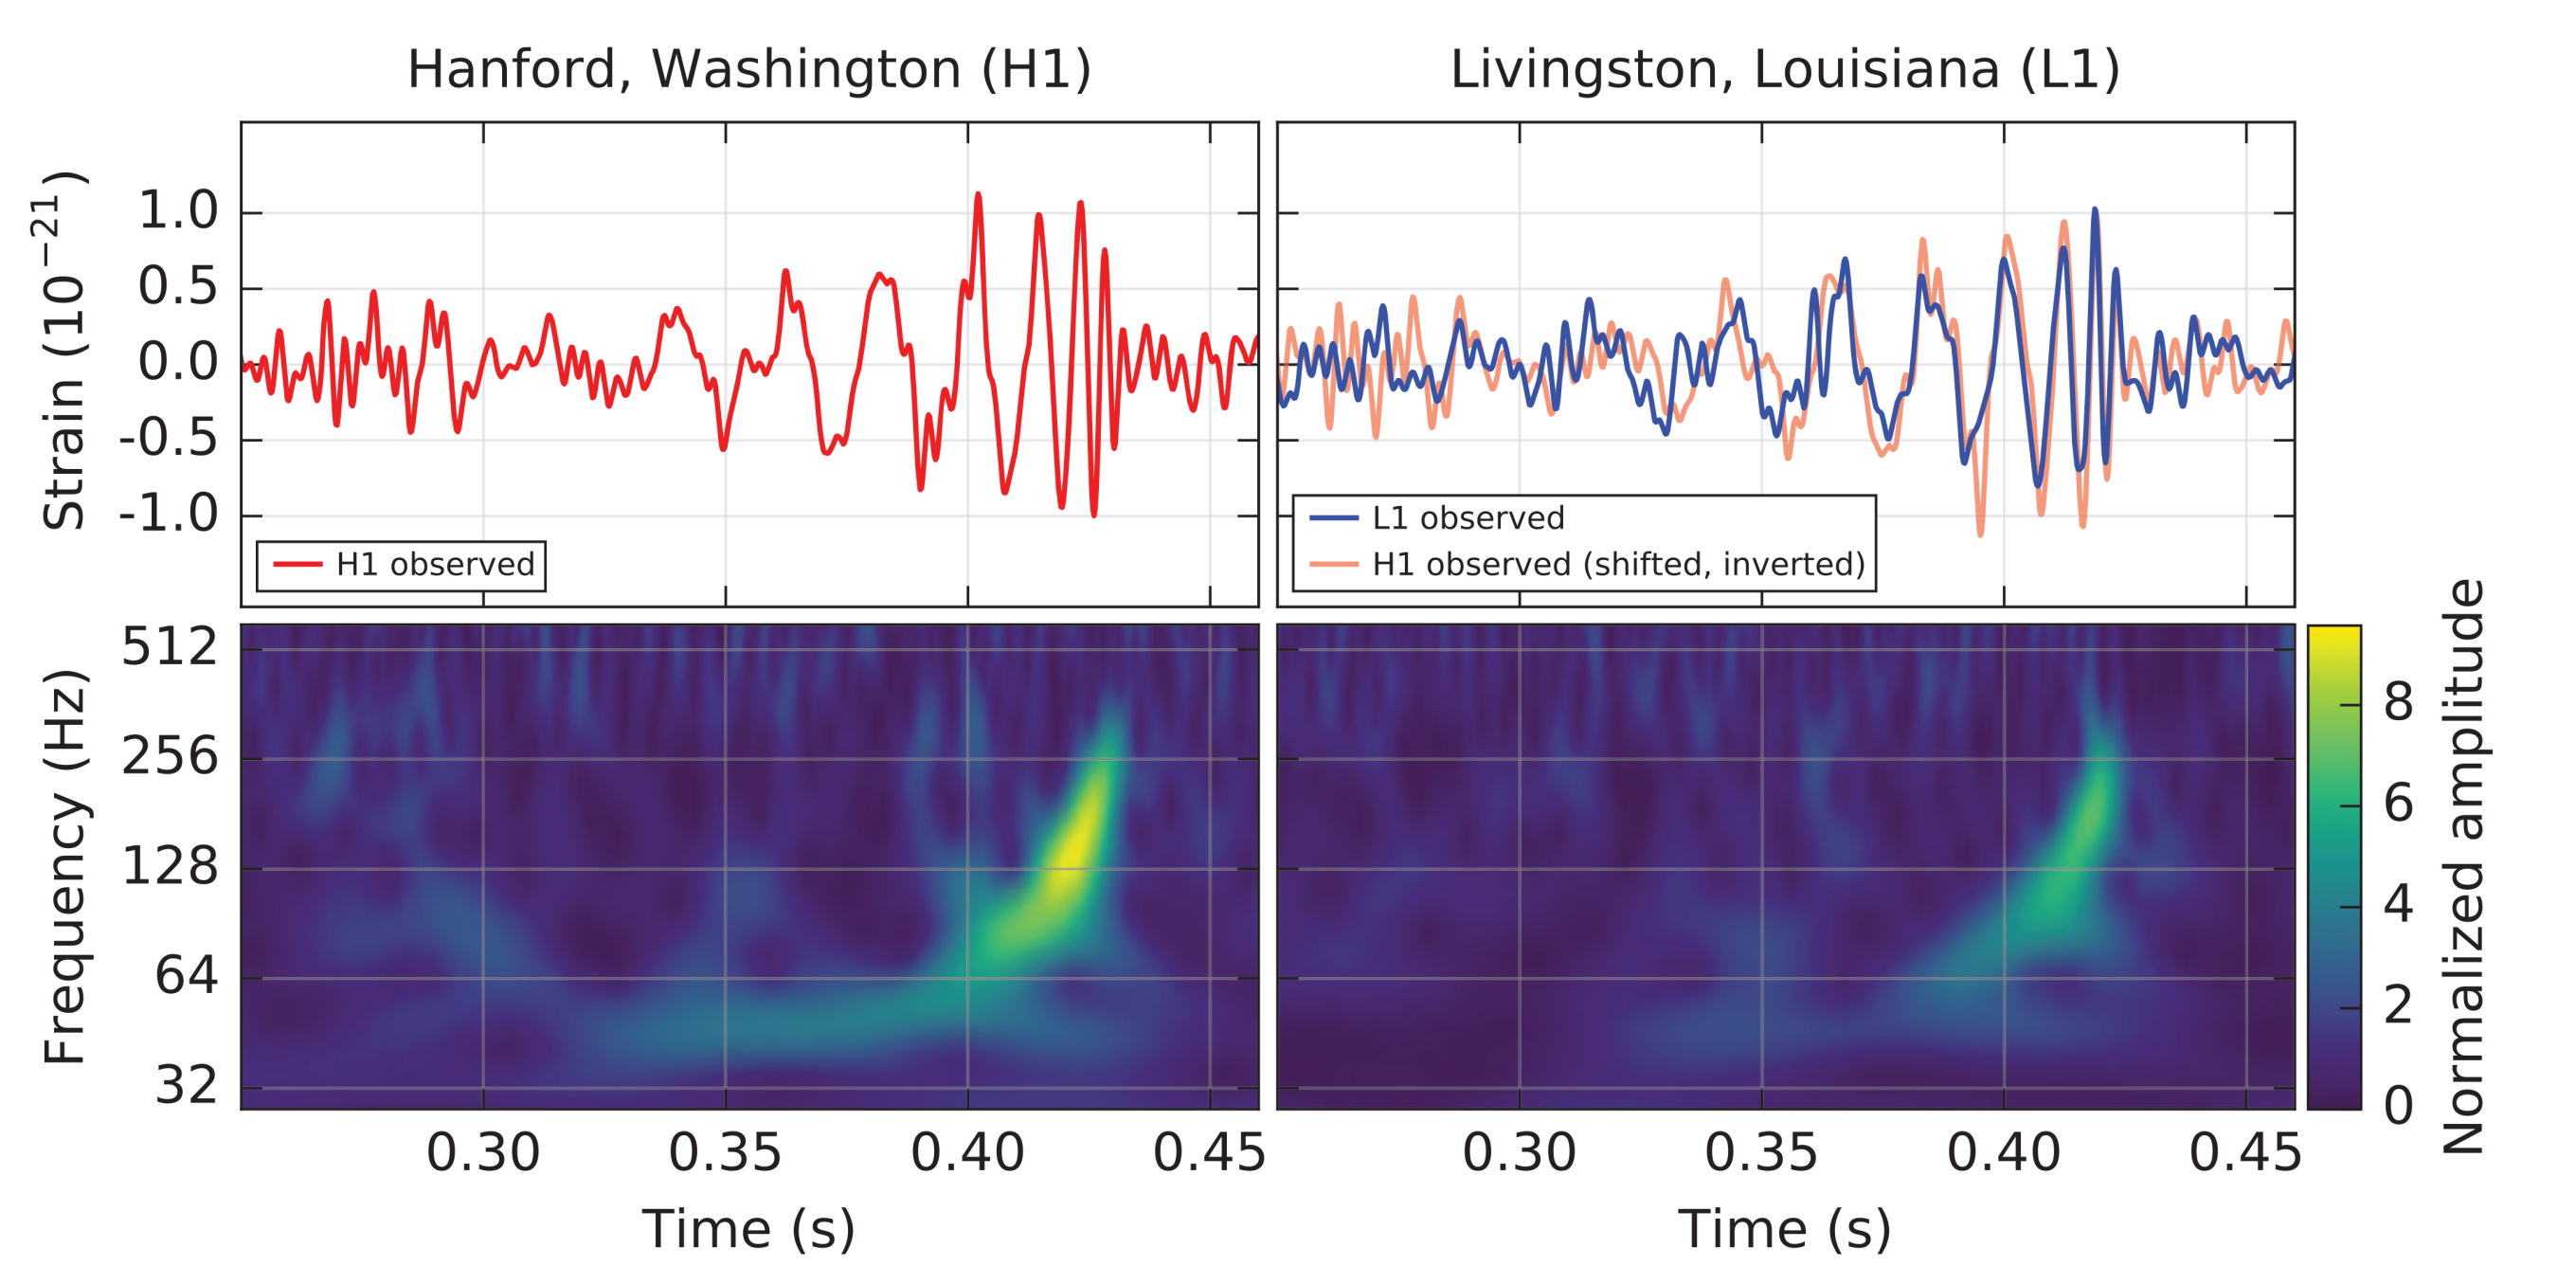
\includegraphics[width=16cm]{the_einstein_telescope/images/gw150914_plot_cropped}}
	\caption{GW150914 as measured at the two LIGO sites, H1 (\emph{left column}) and L1 (\emph{right column}) shifted by \SI{7}{\milli\second} and inverted to make up for the detectors' relative position and orientation. Strain (\emph{top row}) and spectogram (\emph{bottom row}). The data is bandpassed from \SI{35}{\hertz} to \SI{350}{\hertz} for visualization. Adapted from \cite{PhysRevLett.116.061102}.}
	\label{fig:einstein_telescope:gw150914}
\end{figure}	

\begin{figure}
	\centering
	\makebox[\textwidth]{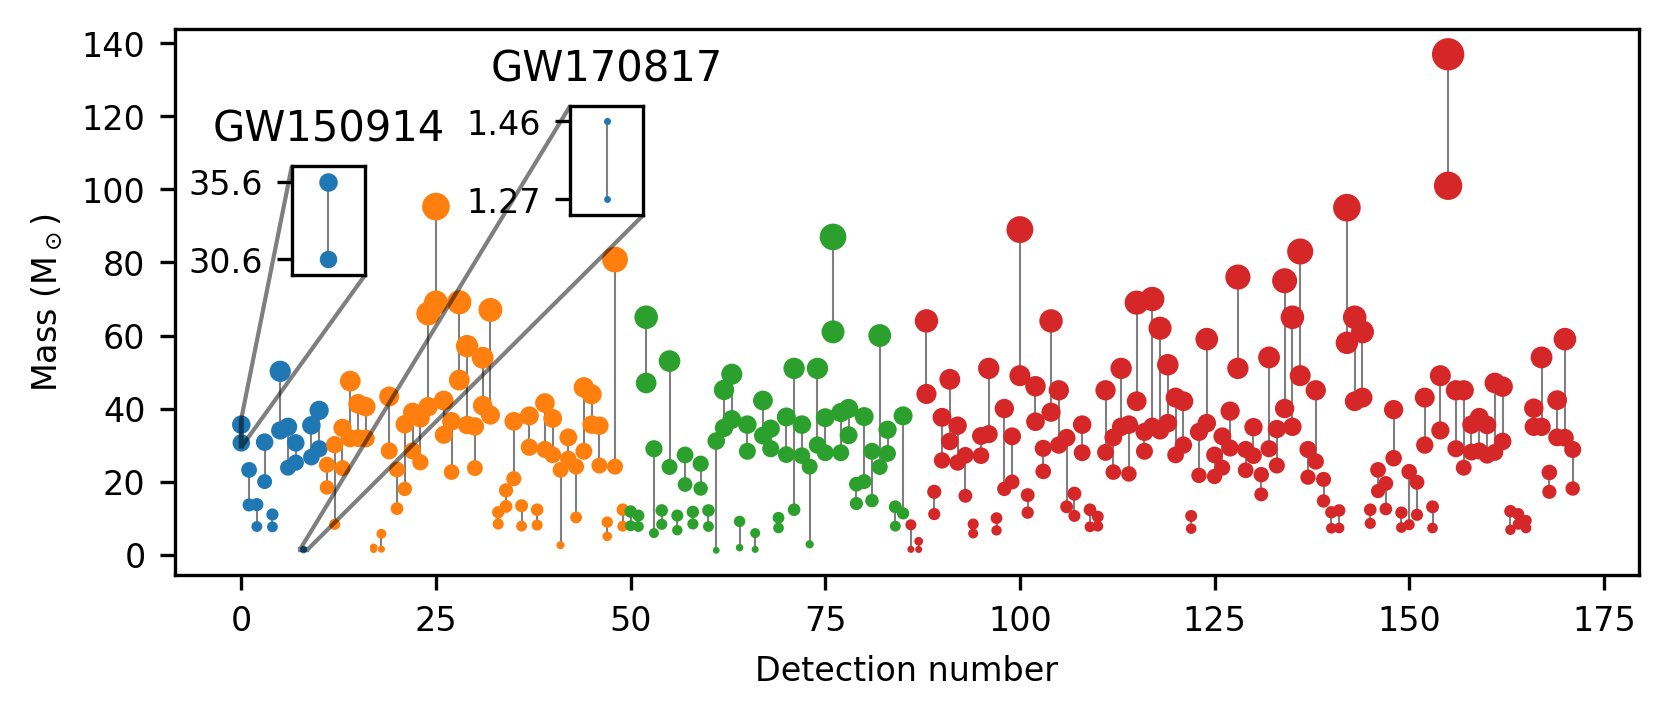
\includegraphics[width=15cm]{theory_of_gravitational_waves/images/population/population}}
	\caption{CBCs observed by LIGO, Virgo and KAGRA in their four observing runs, each plotted in a different color. Each merger is represented as two dots denoting the two component masses (in both y-value and dot size). Data from \cite{PhysRevX.9.031040, PhysRevX.11.021053, PhysRevX.13.041039, theligoscientificcollaboration2025gwtc40updatinggravitationalwavetransient}, uncertainties are not plotted.}
	\label{fig:einstein_telescope:population}
\end{figure}

This detection principle is employed with great success at LIGO, which consists of two interferometers, H1 and L1, separated by \SI{3000}{\kilo\meter}. These have arm lengths of \SI{4}{\kilo\meter} and \SI{90}{\degree} opening angles. The two sites allow for the rejection of false signals via coincident detection ($<\SI{10}{\milli\second}$, the time-of-flight between the two detectors). LIGO achieved the first direct detection of a GW signal on September 14th, 2015 \cite{PhysRevLett.116.061102} resulting in a Nobel prize award in 2017 \cite{nobel2017}. The signal was identified as a BBH merger with masses $36^{+5}_{-4}\,\SI{}{\solarmass}$ and $29^{+4}_{-4}\,\SI{}{\solarmass}$ and with a luminosity distance of $410^{+160}_{-180}\,\SI{}{\mega\parsec}$. GW signals are conventionally labeled based on their arrival time, so GW150914 in this case. See the measured signal in Fig.~\ref{fig:einstein_telescope:gw150914}. So far, the LIGO, Virgo and KAGRA observatories have made more than 200 confident GW detections in the span of four observing runs \cite{PhysRevX.9.031040, PhysRevX.11.021053, PhysRevX.13.041039, theligoscientificcollaboration2025gwtc40updatinggravitationalwavetransient}. The majority of these are black hole mergers. BNS mergers are identified based on the component masses which have to be $\lesssim\SI{2}{\solarmass}$. The first direct detection of a neutron star merger was GW170817 \cite{Abbott_2017}. See the signals for which component masses are provided in Fig.~\ref{fig:einstein_telescope:population}.

%\begin{figure}
%	\centering
%	\makebox[\textwidth]{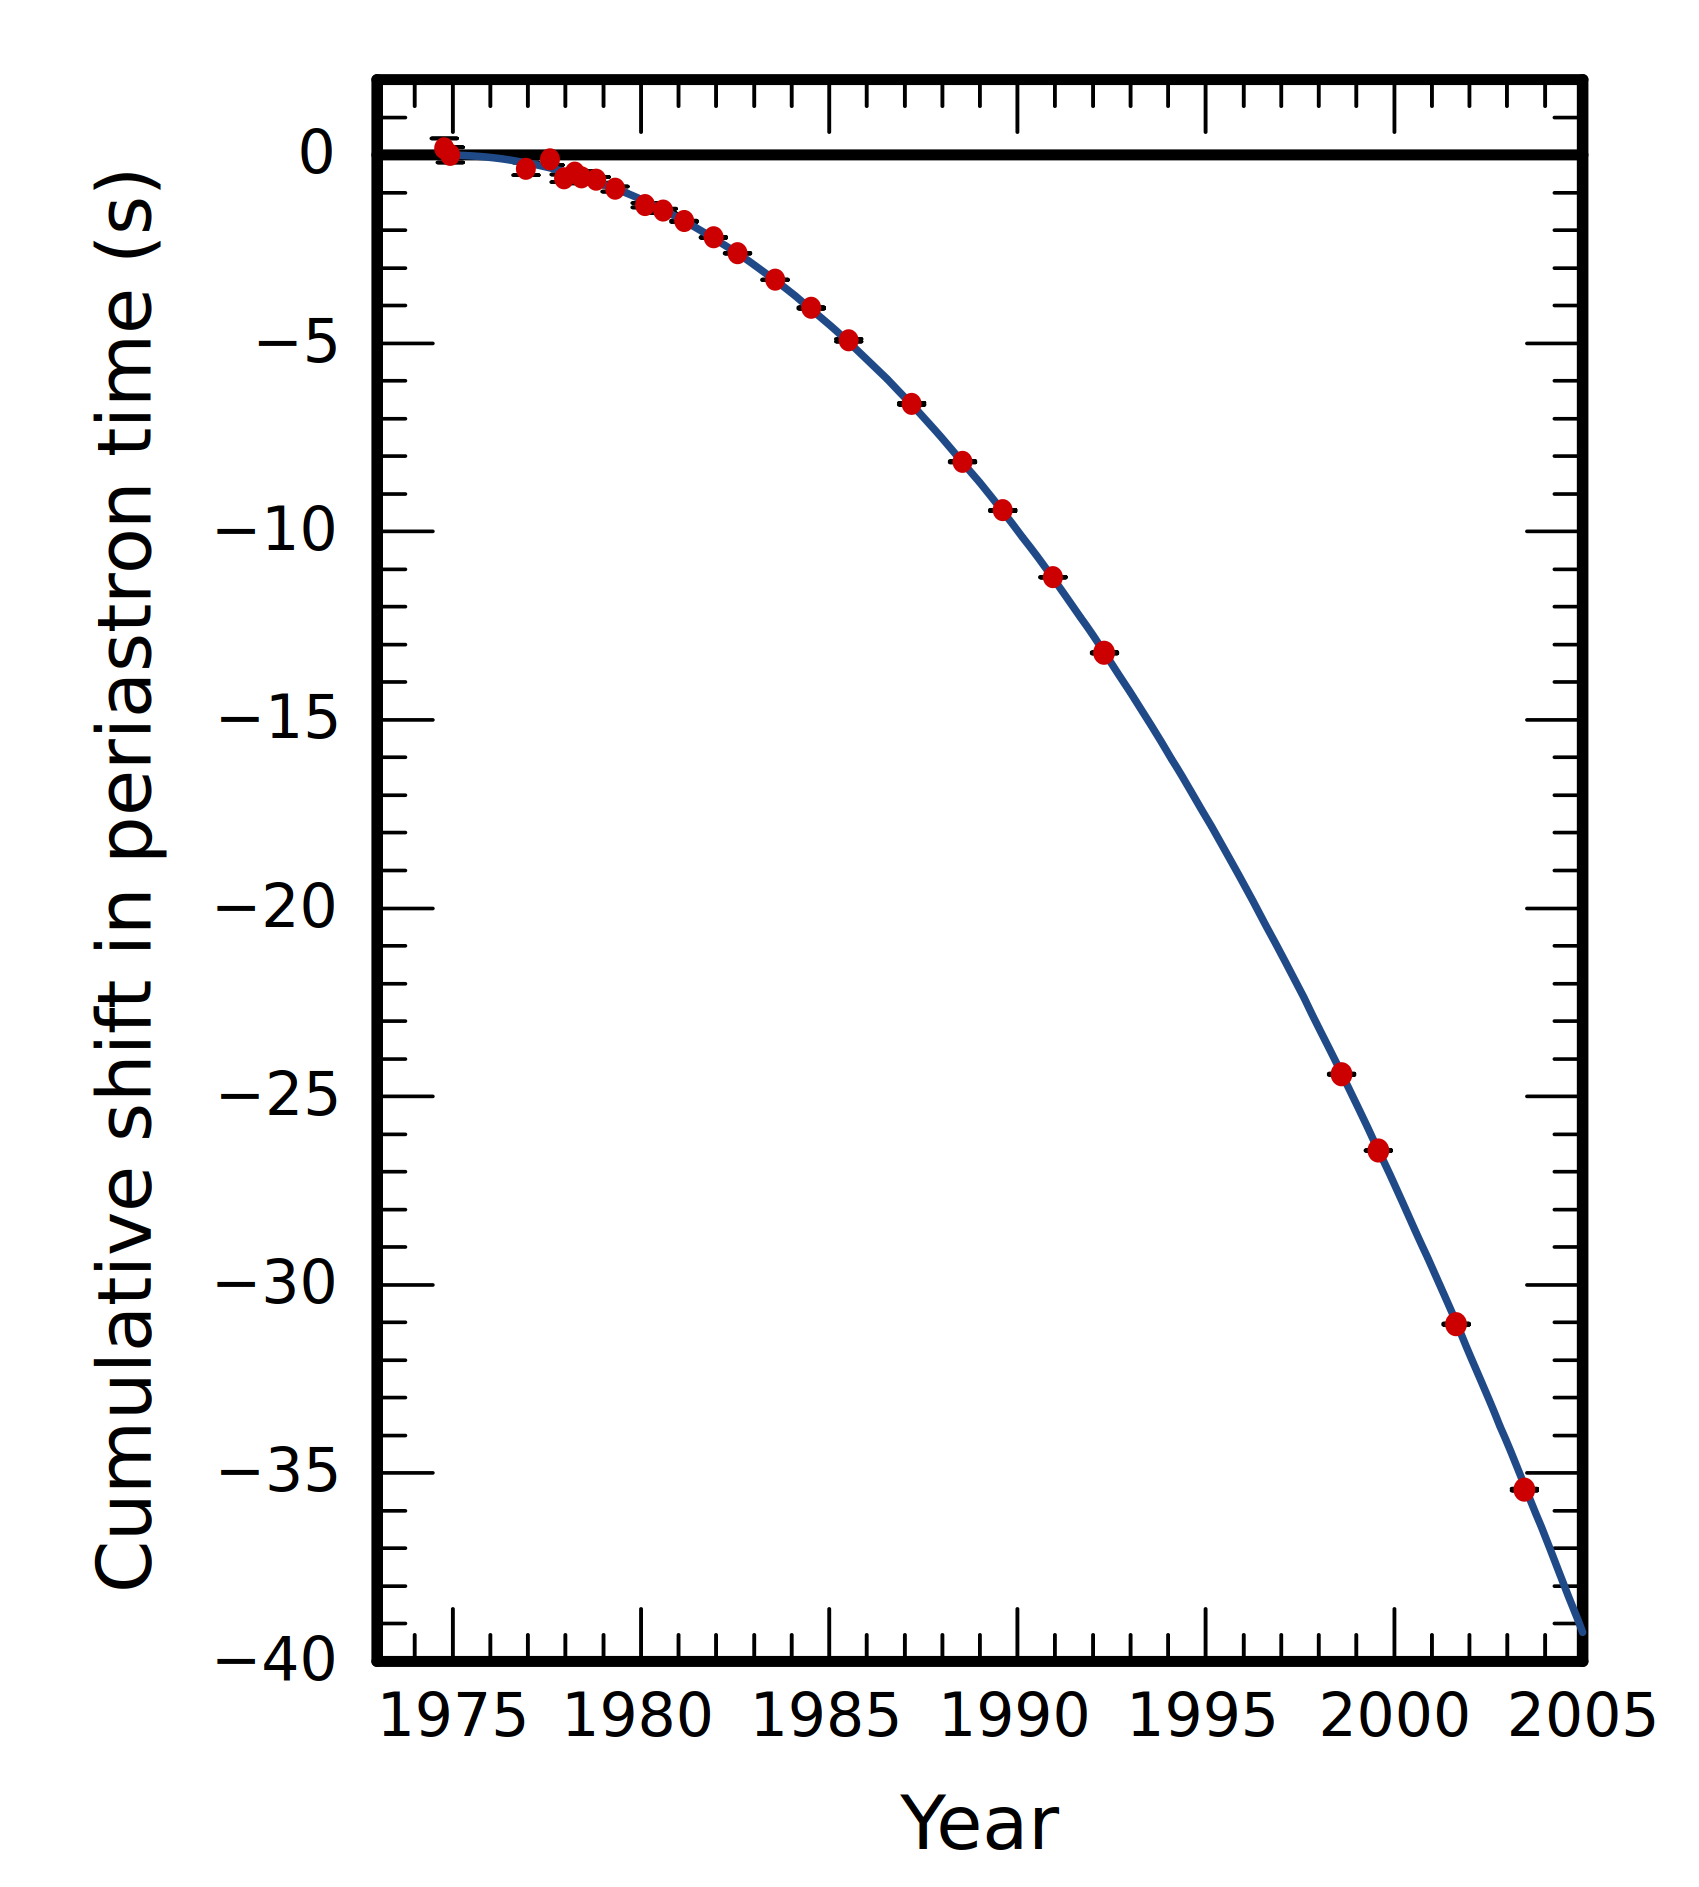
\includegraphics[width=8cm]{the_einstein_telescope/images/hulse_taylor_wiki}}
%	\caption{}
%	\label{fig:einstein_telescope:hulse_taylor}
%\end{figure}	

%\begin{figure}[p]
%	\centering
%	\makebox[\textwidth]{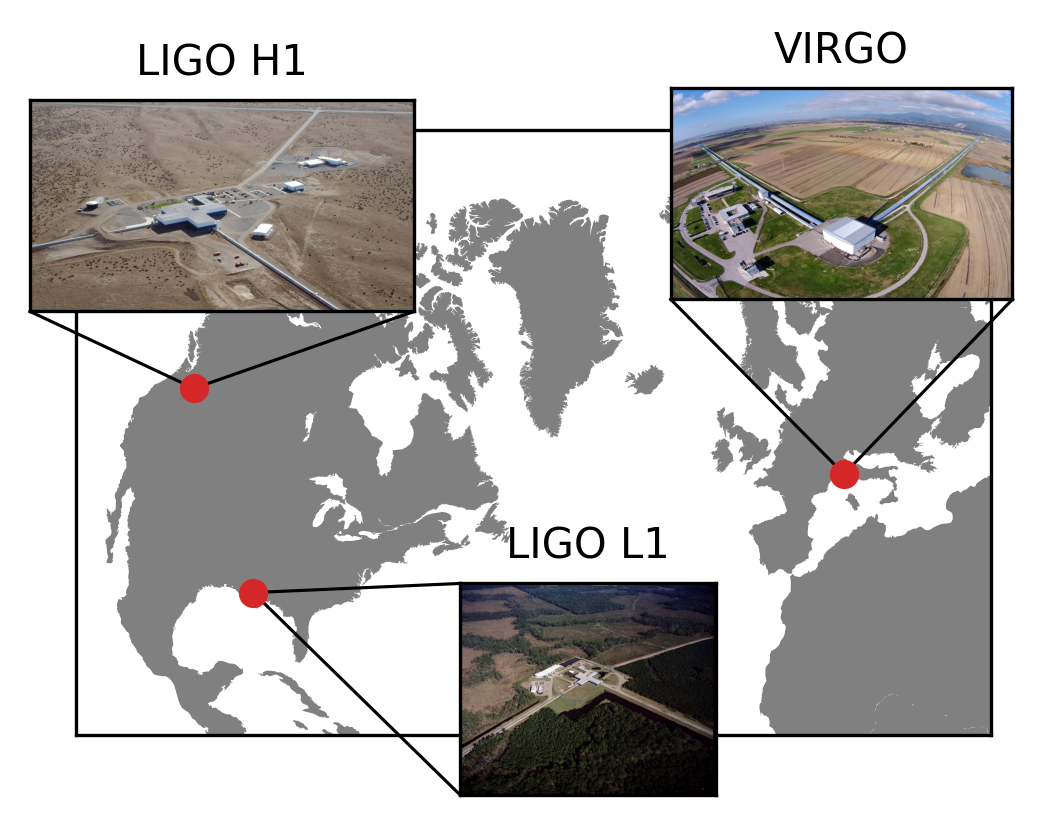
\includegraphics[width=7cm]{the_einstein_telescope/images/2nd_gen_detectors/LIGO_VIRGO}}
%	\caption{Positions of the LIGO and Virgo observatories.}
%	\label{fig:einstein_telescope:2nd_gen}
%\end{figure}	

\section{Conceptual Design}

% 10km arms
% underground -> better sensitivity
% triangle -> all sky coverage, null stream
% xylophone -> LF HF optimized
% candidates are Meuse-Rhine Euregio, or Sardinia

The Einstein Telescope (ET) aims for an increase in sensitivity of a factor ten compared to second-generation detectors, especially in the low frequency regime $\pazocal{O}(\SI{1}{\hertz})$.
To this end, the arm length will be increased to \SI{10}{\kilo\meter} yielding an overall sensitivity increase. To improve the low frequency sensitivity, where noise is mostly seismic, ET will be built \SI{200}{\meter} to \SI{300}{\meter} underground.
A detailed description of the latest ET technical design is provided by \cite{ET-0007C-20}.\footnote{It should be mentioned that this technical report is rather old as of now. In particular, it focuses solely on a triangular configuration of three nested detectors with \SI{60}{\degree} opening angles. However, the detector geometry is currently debated with 2L configurations being investigated as well (two detectors with \SI{90}{\degree} opening angles) \cite{Branchesi_2023}.}

\begin{figure}
	\centering
	\makebox[\textwidth]{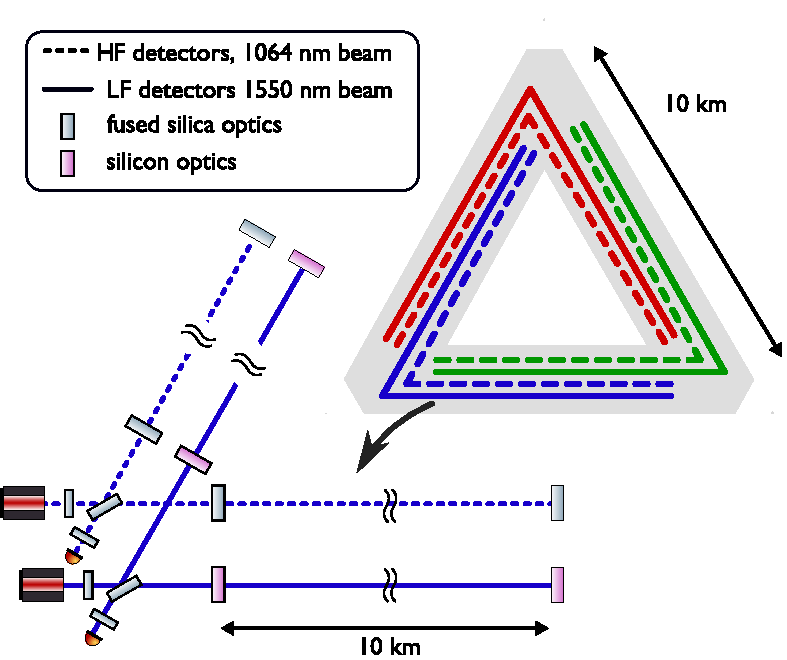
\includegraphics[width=10cm]{the_einstein_telescope/images/ET_triangle_01}}
	\caption{The ET xylophone design. Three detectors arranged in a triangular shape each consisting of a LF and HF interferometer. 
	ET-LF will feature a \SI{1550}{\nano\meter} laser wavelength and silicon optics, while ET-HF will employ a \SI{1064}{\nano\meter} laser with fused silica optics, similar to LIGO and Virgo. 
	Taken from \cite{Rowlinson_2021}.}
	\label{fig:einstein_telescope:xylphone}
\end{figure}

ET will consist of three nested detectors with \SI{60}{\degree} opening angles, arranged in a triangular pattern. 
This allows for better sky coverage at a slight sensitivity cost for interferometers with opening angles $\gamma<\SI{90}{\degree}$ (corresponding to the factor $\sin\gamma$ in Eqs.~\ref{eq:einstein_telescope:antenna_functions}). The arrangement is equally sensitive to both GW polarizations.
Each detector will comprise two interferometers, one optimized for low frequencies of \SI{3}{\hertz} to \SI{30}{\hertz} (ET-LF) and one for high frequencies \SI{30}{\hertz} to \SI{10}{\kilo\hertz} (ET-HF). This is called the \emph{xylophone} configuration. See a schematic in Fig.~\ref{fig:einstein_telescope:xylphone}. 

% noise
% quantum noise -> light power
% thermal noise -> LF: cryogenic cooling, silicon optics
% newtonian noise + seismic noise -> 

\begin{figure}
	\centering
	\makebox[\textwidth]{
		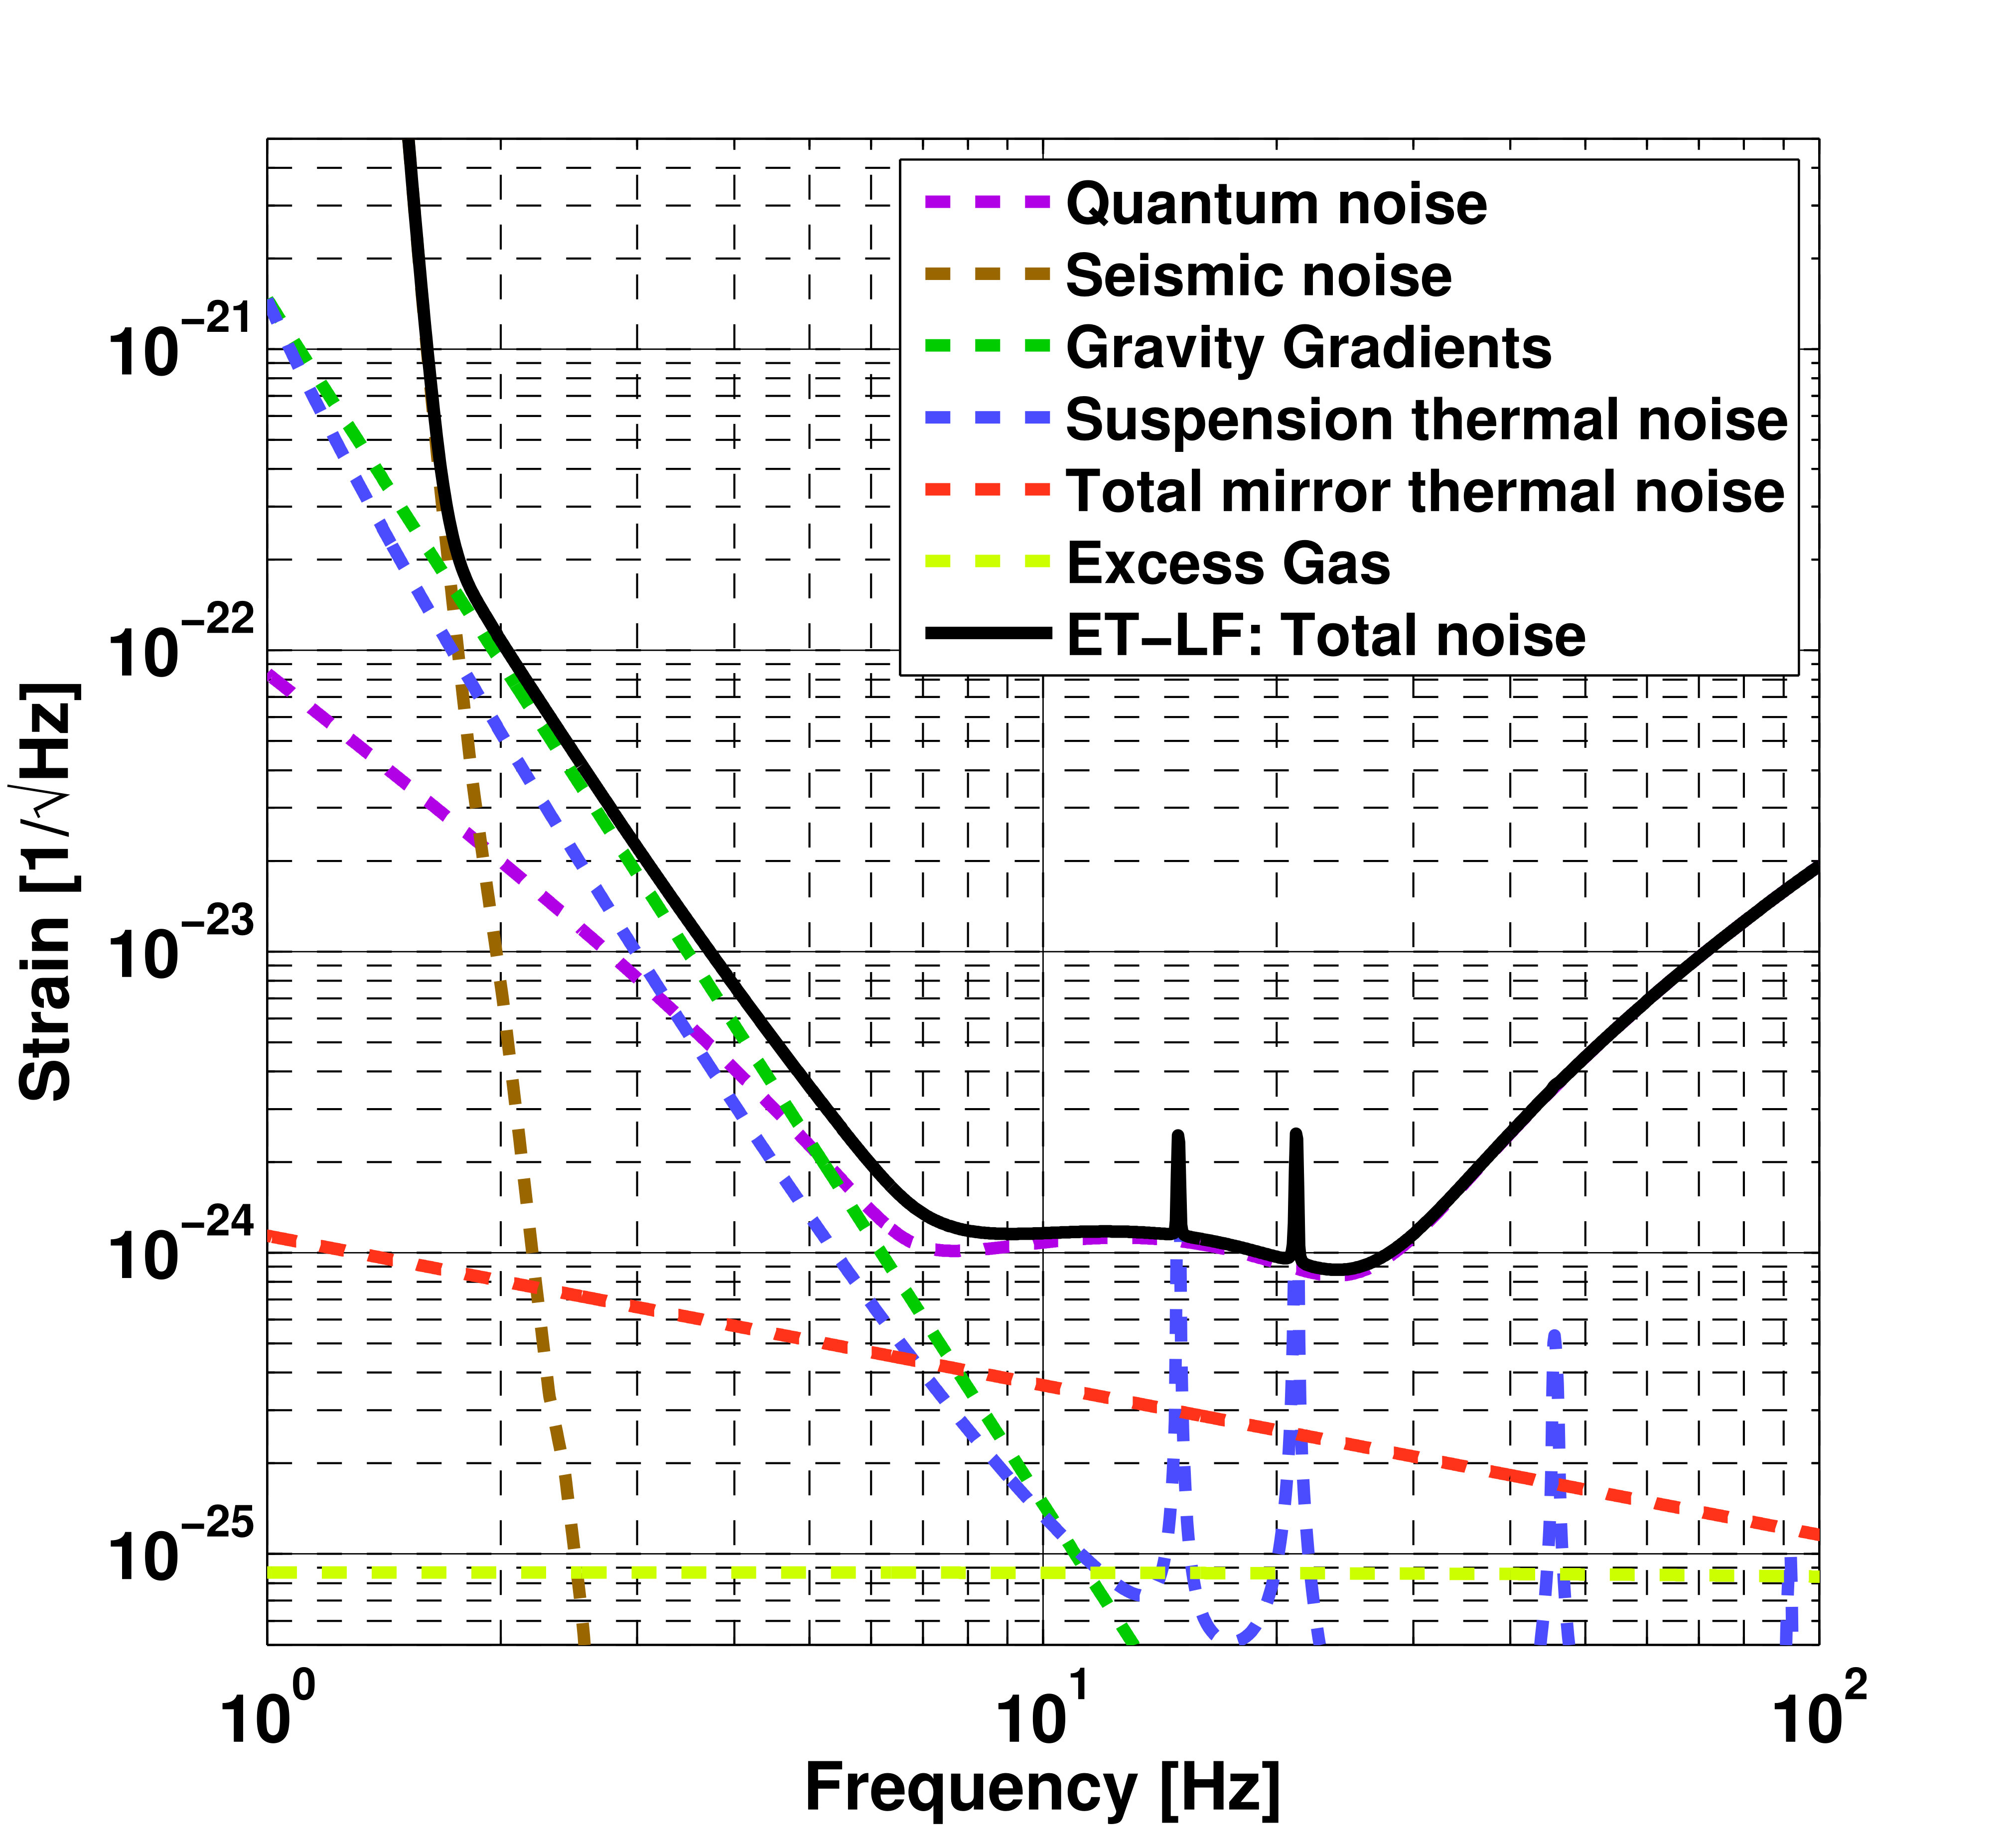
\includegraphics[width=8cm]{the_einstein_telescope/images/ETD_LF3.png}
		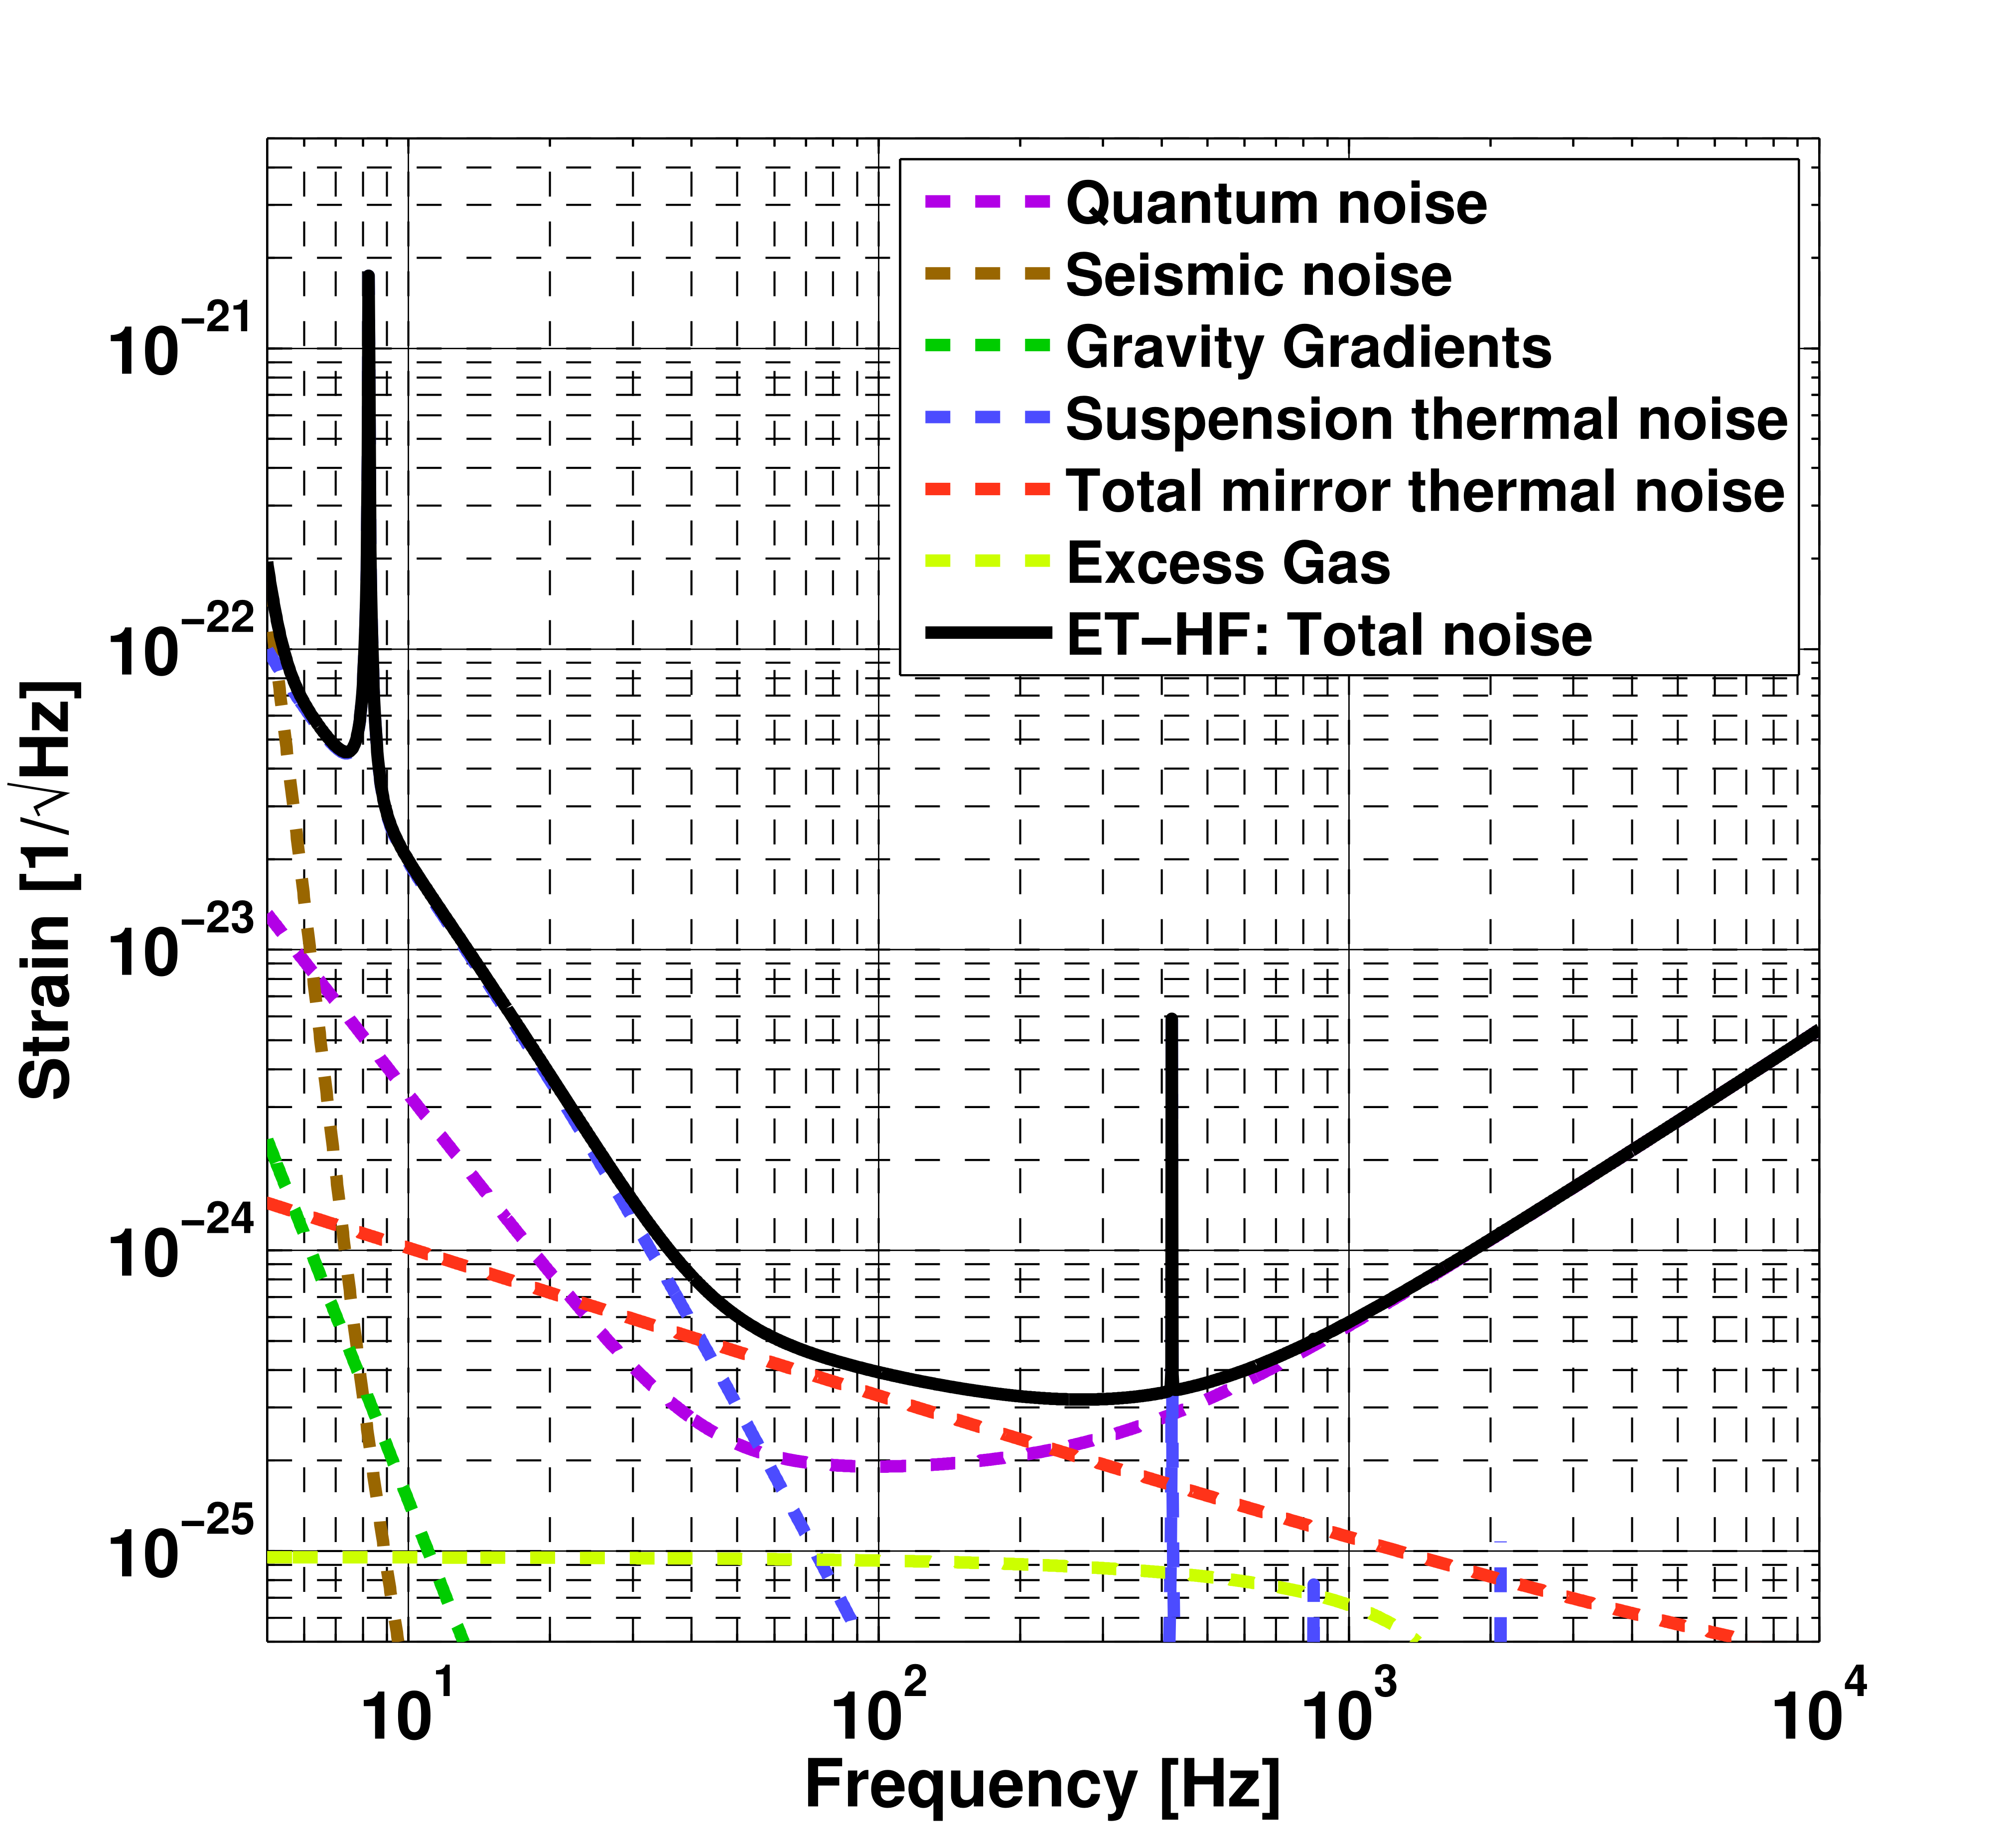
\includegraphics[width=8cm]{the_einstein_telescope/images/ETD_HF3.png}
	}
	\caption{Noise budgets for the ET-LF (left) and ET-HF (right) interferometers. The individual sources (dotted) and the total noise taken as their quadrature sum (black). The label \enquote{Gravity gradients} denotes Newtonian noise. Excess gas noise stems from residual gas in the beam tubes. Taken from \cite{Hild_2011}.}
	\label{fig:einstein_telescope:noise_budget}
\end{figure}

This configuration is useful because the main noise contribution for these instruments, the \emph{quantum noise}, behaves differently at low and high frequencies. This type of noise is caused by individual quanta of light, \emph{i.e.}\ photons, and has two components. The \emph{shot noise} results from the Poisson statistics of the total number of photons detected and dominates at high frequencies. The \emph{radiation pressure noise} arises from the momentum transfer of individual photons to the mirrors upon reflection. Fluctuations in the photon number therefore induce random displacements of the mirrors. This noise dominates at low frequencies. 

These two contributions scale oppositely with laser power: increasing the laser power reduces shot noise but increases radiation pressure.
ET-HF mitigates shot noise by operating with a higher arm cavity power of \SI{3}{\mega\watt}, while ET-LF suppresses radiation pressure by reducing the power to \SI{18}{\kilo\watt}. Compare this to the LIGO interferometers which balance both noise contributions by choosing \SI{750}{\kilo\watt}. In both ET-LF and ET-HF, radiation pressure can be further reduced by employing heavier test masses of \SI{200}{\kilo\gram} instead of \SI{40}{\kilo\gram} at LIGO.

Another noise source is \emph{thermal noise} due to Brownian motion in the test masses and their suspensions. This limits the instrument's sensitivity in the low frequencies, hence ET-LF will operate at cryogenic temperatures of \SI{10}{\kelvin} to \SI{20}{\kelvin}. The poor low-temperature behavior of fused silica, which is used for the optics of ET-HF, necessitates employing silicon for the ET-LF test masses and suspensions. Since silicon is non-transparent to wavelengths of \SI{1064}{\nano\meter}, the standard for second-generation detectors, which will be used for ET-HF as well, ET-LF will move to a larger laser wavelength of \SI{1550}{\nano\meter}.

As already mentioned, the instrument's low-frequency sensitivity is mainly limited by \emph{seismic noise} and \emph{Newtonian noise}. Both of these stem from seismic ground motion caused by local disturbances such as human activity or wind. Seismic noise describes the vibrations directly induced on the optics and can be shielded by a combination of active and passive isolation systems. ET will employ a multi-stage pendulum suspension system for its mirrors, similar to LIGO and Virgo.

Newtonian noise, on the other hand, describes disturbance of the local gravitational field caused by the mass density fluctuations associated with seismic ground motion and its effect on the test masses. Contrary to seismic noise, Newtonian noise cannot be shielded, which is the main argument for moving the detector \SI{200}{\meter} to \SI{300}{\meter} underground to a sparsely populated region. Candidates include the Euregio Meuse-Rhine and Sardinia \cite{etcandidates}.

ET is set to provide a sensitivity improvement of a factor ten, achieving a targeted sensitivity of \SI{E-24}{\hertz^{-1/2}} and broadening the frequency range down to \SI{3}{\hertz} to \SI{5}{\hertz}, compared to the current detectors' \SI{10}{\hertz} to \SI{20}{\hertz} lower limit.
See the ET noise budget for both interferometers in Fig.~\ref{fig:einstein_telescope:noise_budget}. Plotted here is the noise \emph{amplitude spectral density} (ASD) which is the square root of the \emph{power spectral density} (PSD) and is related to the root-mean-square noise amplitude at each frequency. (Ch.~\ref{sec:matched_filtering} will introduce these formally.)

\section{Scientific Goals}
 
 % -- intro paragraph --
 % black hole properties (origin (ABH, PBH -> dark matter candidate), evolution?, population)
 % neutron star properties (interior structure (QCD), population)
 % sky localization -> multi messenger (electro magnetic or neutrino follow-up from BNS)
 % new sources (CCSNe, stochastic background)
 
With its increased sensitivity, ET will detect large numbers of CBCs up to high redshifts and with unprecedented precision. In numbers that is \SI{E+5}{\nothing} to \SI{E+6}{\nothing} BBH and \SI{E+4}{\nothing} BNS signals annually \cite{abac2025scienceeinsteintelescope}. This has the potential for advances in astrophysics, cosmology and fundamental physics. For a full discussion of ET's main science cases, see \cite{ET-0007C-20, abac2025scienceeinsteintelescope}.

ET will enable the study of the stellar black hole and neutron star populations, including their mass and spin distributions, their evolution with redshift, and their formation mechanisms. ET will probe black holes beyond the epoch of star formation, possibly uncovering black holes of primordial origin. These are hypothetical non-stellar black holes, formed in the high-density conditions of the early universe, which are proposed as a dark matter candidate.

High precision measurements of CBC signatures will provide accurate tests of GR, particularly in the extreme domain during the merger phase of BBHs. Similarly, high-precision BNS signatures allow for the study of quantum chromodynamics at ultra-high density, and of possible phase transitions in the neutron star core.

ET's excellent sky coverage and sensitivity make it capable of localizing GW sources with remarkable precision. This opens the opportunity for multi-messenger astronomy, where non-GW observatories probe the source's sky location for electromagnetic or neutrino follow-ups. This is especially important for mergers involving a neutron star, which can emit both GWs and electromagnetic radiation in a kilonova \cite{Abbott_2017_kilonova}. 

Besides CBC signals, ET may detect other types of GW sources. These include signals from core collapse supernovae, continuous signals emitted by isolated rotating neutron stars, and possibly the stochastic GW background.



\chapter{Low-Latency Searches}
\label{sec:matched_filtering}
% Intro abaout ET computing infrastructure:
% low latency searches for cbcs
% matched filtering -> trigger
% bayesian inference -> parameters
% masses, etc: Data monitoring
% sky-localization: Multi-messenger

GW signals are identified in detector data with search algorithms, returning (multiple) GW candidates. 
These are called \emph{online} if they produce real-time or low-latency triggers on the data as they are taken and \emph{offline} else.
In the observing runs of the second-generation detectors, online searches were instrumental for data monitoring and multi-messenger astronomy \cite{Nitz_2018}. 
These searches rely upon matched filtering to produce real-time triggers, and focused Bayesian inference for subsequent parameter estimation. 

This chapter states the problem of identifying GW signals in the detector data formally. It introduces matched filtering, and its shortcomings for low-latency trigger generation in the high event-rate conditions of ET, motivating the investigation of alternative or complementary methods, \emph{e.g.}\ machine-learning based. The chapter's main source is \cite{10.1093/acprof:oso/9780198570745.001.0001}.

\section{Problem Setup}

For a given detector stream, a search algorithm will return a number of time triggers corresponding to identified GW events. The returned time will usually correspond to the CBC merger time and should be accompanied by some confidence measure. 

The detector strain is a function of time $s(t)$, and is made up of two additive components, the instrument noise $n(t)$ and a possible signal contribution $h(t)$:
\begin{equation}
	s(t) = n(t) + h(t).
\end{equation}
For now, the signal contribution will be assumed to either vanish or correspond to a single CBC signal with merger time $t_\text{coa}$. The generalization to multiple signals will be explored later.
If a signal is present, it will induce a strain according to Eq.~\ref{eq:einstein_telescope:strain} resulting in amplitudes of order \SI{E-21}{\nothing} or smaller.
Usually $|h(t)| \ll |n(t)|$, making the identification of this signal inside the much larger noise non-trivial.

The noise strain can be described as a statistical process, which is stationary, \emph{i.e.}, its properties do not change over time. This process is characterized by the noise power spectral density $S_n(f)$ (PSD). The PSD is in turn related to the Fourier transform of the noise strain $\tilde{n}(f)$. In particular, through the expectation value $\langle\cdot\rangle$ of the Fourier components:
\begin{equation}
	\label{eq:matched_filtering:PSD_definition}
	\langle\tilde{n}^*(f)\,\tilde{n}(f')\rangle 
	= \delta(f-f')\,\frac{1}{2}S_n(f).
\end{equation}	
Here, $\delta$ denotes the Dirac delta function. Notice that since $n$ is real, $\tilde{n}(-f)^* = \tilde{n}(f)$ and therefore $S_n(-f) = S_n(f)$. The factor $1/2$ is inserted such that the mean squared noise $\langle n(t)^2\rangle$ is obtained by integrating $S_n(f)$ over the physical range of $f\geq0$, rather than from $-\infty$ to $\infty$:
\begin{align}
	\label{eq:matched_filtering:stationarity}
	\langle n(t)^2\rangle &=
	\langle n^*(t)\,n(t)\rangle_{\,t=0} \\
	&= \int_{-\infty}^\infty\mathrm{d}f\mathrm{d}f'\,
	\langle\tilde{n}^*(f)\tilde{n}(f')\rangle \\
	\label{eq:matched_filtering:definition}
	&=  \frac{1}{2}\int_{-\infty}^\infty\mathrm{d}f\,S_n(f) \\
	&= \int_0^\infty\mathrm{d}f\,S_n(f),
\end{align}
where Eq.~\ref{eq:matched_filtering:stationarity} makes use of stationarity, and Eq.~\ref{eq:matched_filtering:definition} follows from the PSD definition (Eq.~\ref{eq:matched_filtering:PSD_definition}). To emphasize this fact, the PSD is called \emph{single-sided} if defined like this. This convention will be used in the rest of this work.

\section{Matched Filtering}

If the shape the signal strain can take on is known (as is the case for CBC signals), matched filtering can be applied. The basic idea is to \enquote{filter out} the noise contribution of the total detector strain by multiplying with a filter function and integrating over the observation time $T$. Although not necessarily optimal, this technique works for a filter that is equal to the signal:
\begin{equation}
	\frac{1}{T}\int_0^T \mathrm{d}t s(t)h(t) = \frac{1}{T}\int_0^T \mathrm{d}t h^2(t) + \frac{1}{T}\int_0^T \mathrm{d}t n(t)h(t).
\end{equation}
Here, the first integrand on the right-hand side is positive definite and the first summand will be constant for large $T$ while the second summand which is the noise contribution will approach zero.

This procedure can be formalized by defining the filtered detector strain as
\begin{equation}
	\label{eq:matched_filtering:filtered_strain}
	\hat{s} = \int_{-\infty}^\infty \mathrm{d}t\,s(t)K(t),
\end{equation}
for some filter function $K(t)$. The \emph{optimal} or \emph{matched} filter should maximize the \emph{signal-to-noise ratio} (SNR) of $\hat{s}$. The SNR is taken as the ratio of $S$, the expected value of $\hat{s}$ if a signal is present, and $N$, the root mean square of $\hat{s}$ if \emph{no} signal is present. That is,
\begin{equation}
	S = \langle\hat{s}\rangle \quad \text{and} \quad 
	N^2 = [\langle\hat{s}^2\rangle - \langle\hat{s}\rangle^2]_{h(t) = 0}.
\end{equation}
Requiring $\langle n(t)\rangle = 0$ and making use of the PSD definition (Eq.~\ref{eq:matched_filtering:PSD_definition}), the SNR takes the form,
\begin{equation}
	\label{eq:matched_filtering:snr}
	\frac{S}{N} 
	= \frac{\int_{-\infty}^\infty \mathrm{d}f\,\tilde{h}(f)\tilde{K}^*(f)}
	{\sqrt{\int_{-\infty}^\infty \mathrm{d}f\frac{1}{2}S_n(f)|\tilde{K}(f)|^2}}.
\end{equation}
Skipping the derivation, the solution to the variational problem that is to find the optimal filter $K(t)$ maximizing $S/N$ is given by,
\begin{equation}
	\tilde{K}(f) \sim \frac{\tilde{h}(f)}{S_n(f)}.
\end{equation}
See \cite{10.1093/acprof:oso/9780198570745.001.0001} for proof.
Notice that for white noise $S_n(f) = 1$ and the optimal filter will be equal to the signal which corresponds to the naive approach taken earlier. 

The search of the optimal filter is simply brute forced. To this end, a \emph{template bank} of possible waveforms is constructed, covering the whole parameter space at a reasonable resolution. The template that yields the maximum SNR while exceeding some threshold will be the GW signal candidate. This is a strongly simplified search pipeline. A \emph{full} pipeline is provided by the PyCBC software package \cite{alex_nitz_2023_10013996, Usman_2016}.  

In practice, the expectation value $S=\langle\hat{s}\rangle$ and therefore the SNR, $S/N$, is obviously not available as it requires knowledge of the true GW signal $h(t)$. Instead, the SNR is calculated as $\rho = \hat{s}/N$, which depends on the full detector strain $s(t)$. This gives a \enquote{noisy} estimate of $S/N$, reflecting the instrument noise statistics. On average, $\langle\rho\rangle = S/N$.

Matched filtering will return a time trigger, \emph{e.g.}\ the merger time of the template, and the corresponding SNR serves as a confidence measure. As a bonus, the optimal template gives a rough estimate of the signal parameters.
The SNR corresponding to the optimal filter reads,
\begin{equation}
	\label{eq:matched_filtering:optimal_snr}
	\left(\frac{S}{N}\right)_\text{opt}
	= 2\sqrt{\int_0^\infty\,\mathrm{d}f\,\frac{|\tilde{h}(f)|^2}{S_n(f)}}.
\end{equation}
This is often and will also in this work be called the SNR of the signal $h(t)$ for a given noise PSD. Note that this is not literally the SNR of the signal $h(t)$ with respect to the detector noise $n(t)$, 
but rather the SNR of the optimally filtered detector strain $\hat{s}$. Still this wording is used because it gives a sense of the detectability or loudness of a signal. 
To give a sense of scale: for a random template the SNR will be $2$ on average.
The PyCBC matched filtering pipeline typically disregards templates with SNR values below a threshold of $5.5$ \cite{Usman_2016}.

\section{Challenges and Thesis Motivation}

% -- problems -- 
% high sensitivity 
% lots of signals 10⁵ to 10⁶ BBHs and 10⁴ BNS
% long signal duration
% overlap (maybe some numbers)

As already mentioned, the high sensitivity of ET will introduce challenges for online GW searches with matched filtering. The problem is less an increase in data volume from the six interferometers (plus auxiliary channels) compared to the existing second-generation network. Rather, it is the quantity of valuable scientific information hidden in the data that will grow, and the increased computational power needed to extract it.

The problem is twofold: The increased sensitivity results in longer-duration signals, and a larger event-rate. Combined, this introduces the added challenge of signal overlap. 

The increased CBC signal durations stem exclusively from ET's improvements in the low-frequency range. CBC signals are chirp-like, and will enter the ET sensitivity band earlier thus being detectable for longer. An approximation can be made by recalling that the binary's orbital frequency $\omega$ is related to the time to coalesce $\tau$ through Eq.~\ref{eq:gravitational_waves:cbc_freq}, and that the GW signal frequency is $f=\omega/\pi$. Putting both together, and rearranging yields,
\begin{equation}
	\label{eq:matched_filtering:signal_duration}
	\tau \approx \SI{2.18}{\second}\,
	\left(\frac{\SI{1.21}{\solarmass}}{\pazocal{M}}\right)^\frac{5}{3}\,
	\left(\frac{\SI{100}{\hertz}}{f_\text{lower}}\right)^\frac{8}{3},
\end{equation}
the remaining signal duration once a frequency of $f_\text{lower}$ is reached.
GW150914 with chirp mass \SI{30}{\solarmass} entered LIGO's sensitivity band at \SI{20}{\hertz} and lasted for less than \SI{1}{\second}. In contrast, it would have entered ET's band around \SI{4}{\hertz}, lasting for a whole minute. This effect is even more pronounced for low-mass inspirals such as BNS mergers. GW170817 had a chirp mass of \SI{1.2}{\solarmass} and entered the LIGO band at \SI{10}{\hertz}, corresponding to a signal duration of \SI{17}{\minute}. In ET that would be \SI{1}{\hertz} and total signal-duration of more than \SI{24}{\hour}.
% TODO: check numbers

ET is expected to detect \SI{E+5}{\nothing} to \SI{E+6}{\nothing} CBC signals annually. As these events occur independently of one another, they can be assumed to follow a Poissonian distribution. For a given signal rate $\lambda$, the probability that two events are separated by a time-duration of less than $\Delta t$ is,
\begin{equation}
	P(\Delta t) = 1 - \e^{-\lambda \Delta t}.
\end{equation}
For the higher estimate of $\lambda = \SI{E+6}{\per\year}$, this means that the majority of all signals, \SI{85}{\percent}, will be separated by less than a minute. A total of \SI{3E+4}{\nothing} signals will be separated by less than one second. Since for BBH signals (which make up the majority of mergers) durations of $\sim\SI{1}{\minute}$ are expected, this high merger rate introduces regular signal overlap. 

% -- challenges for matched filtering --
% template bank explodes 
% offline search works \cite{Relton_2022}
% real time? not clear 

These two effects introduce computational challenges for matched filtering. For one, the increased signal-duration necessitates longer waveform templates. This increases the template banks' memory needs, and slows down the algorithm, which is linear in time complexity with respect to template length. Secondly, the signal overlap, especially for mergers separated by less than one second, breaks the assumption that detector data contains, at most, one signal at any time. 
% that templates are independent of one another. 

These challenges have been addressed in \cite{Relton_2022}. Without adaption, matched filtering turns out to retain accuracy in \emph{offline} GW searches when signals are separated by more than one second, but breaks down for closer signals. The latter case of separations of less than one second will make up a substantial amount of signals in ET. Also, it is not yet clear how \emph{online} searches will perform in ET conditions. This motivates the investigation of alternative methods for low-latency GW searches.

% -- thesis motivation --
% use machine learning
% focus only on BBHs 
% far more frequent (-> more important for data monitoring)
% because BNS complicate searches in two ways:
% day long -> source moves on the sky
% multi-messenger -> need for negative latency alert
% focus on long signals first
% then overlapping

This thesis studies the performance of machine-learning methods for low-latency searches in ET conditions. The scope of this work includes BBH signals only, while BNS mergers will be disregarded. In ET, the expected event rate of BBH mergers is significantly larger than for BNS. The use case of BBH low-latency searches is primarily data monitoring, as opposed to multi-messenger alerts. BNS signals complicate searches in two ways. Their signal-duration is much longer, and their potential for multi-messenger astronomy requires \emph{negative}-latency alerts, where triggers are distributed prior to the signal's merger phase.

\chapter{Machine Learning}
\label{sec:machine_learning}
Machine learning is concerned with the development of statistical algorithms that can \enquote{learn} from data and generalize to unseen data, without being explicitly programmed. One particular class of such algorithms is \emph{neural networks}, originally inspired by the human brain, which have proven highly successful. 
Technically, these fall under \emph{deep learning}, which is a subset of machine learning. Still, the use of deep-learning methods has become so ubiquitous (at least in physics applications) that both these terms are used more or less synonymously. 

Machine learning requires large-scale matrix computations. These can be performed efficiently on graphics processing units (GPUs). This thesis makes use of \emph{PyTorch}~\cite{paszke2019pytorchimperativestylehighperformance}, which is Python-based, to handle these computations. PyTorch also serves as an extensive machine-learning library, which includes models, loss functions and optimizers.
The hardware used in this thesis is provided by the HPC cluster PALMA II of the University of Münster.

% -- thesis motivation --
% use machine learning
% focus only on BBHs because BNS complicate searches in two ways:
% day long -> source moves on the sky
% multi-messenger -> need for negative latency alert
% focus on long signals first
% then overlapping

The investigation of machine-learning methods to complement matched filtering, for low-latency searches in particular, is not novel \cite{George_2018}. Recently, the increased amount of data from the growing second-generation GW observatory network, and the corresponding computational burden has motivated such studies \cite{PhysRevD.100.063015}. The research focuses primarily on convolutional neural networks (CNNs), and finds comparable performance while being far more computationally efficient, which is important for real-time detection.

This chapter introduces the basics of machine learning. This includes artificial neurons, how they are arranged into neural networks, and how these networks are trained to extract relevant information from data. Two architectures will be presented in detail, CNNs and the Transformer~\cite{NIPS2017_3f5ee243}.

\section{Basics}

\begin{figure}
	\centering
	\makebox[\textwidth]{
		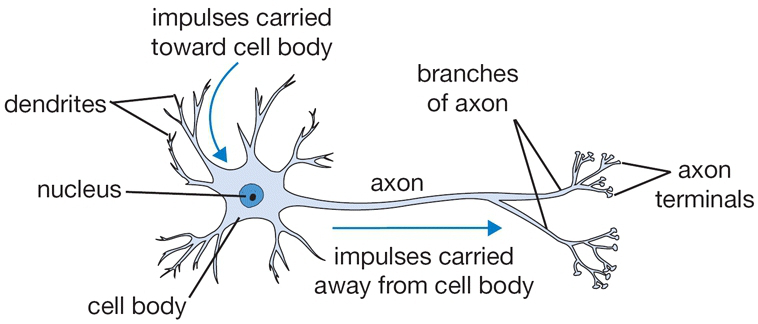
\includegraphics[width=8.5cm,align=c]{machine_learning/images/stanford_neuron}
		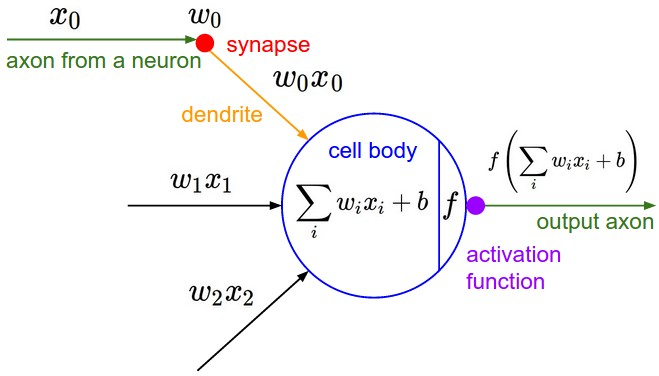
\includegraphics[width=8.5cm,align=c]{machine_learning/images/stanford_perceptron}
	}
	\caption{Drawing of a biological neuron (\emph{left}) and the mathematical model of an artificial neuron (\emph{right}). Taken from \cite{cs231n_neural_networks}.}
	\label{fig:machine_learning:neuron}
\end{figure}

% biological neuron -> artificial neuron
The fundamental building blocks of neural networks are \emph{artificial neurons}. 
These were originally conceived as simplified models of \emph{biological} neurons, excitable nerve cells in the brain, which receive and transmit electrical signals. Such cells consist of multiple dendrites, which carry signals towards the cell body, and one single axon that carries nerve signals away from it. The axon branches into a number of axon terminals, which transmit signals via synapses to the dendrites of other nerve cells. See a drawing in Fig.~\ref{fig:machine_learning:neuron} on the left.

Artificial neurons model this behavior by taking a number of inputs $\vec{x}$, \emph{e.g.}, from other neurons, for which they produce a single output $y$. The neuron assigns weights to each input, modeling the synaptic strength between itself and previous neurons. These weights $\vec{w}$ are \enquote{learnable}, and can be positive (excitatory) or negative (inhibitory). Initial research modeled neurons to always have a binary output, \emph{e.g.} $0$ or $1$. The neuron sums all weighted inputs, and \enquote{fires} if that sum exceeds a certain threshold $t$:
\begin{equation}
	y = \begin{cases}
		1 & \text{if } \vec{x}\cdot\vec{w} > t, \\
		0 & \text{else.}
	\end{cases}
\end{equation}
Artificial neurons were later modified to produce a continuous output, 
\begin{equation}
	y = f(\vec{x}\cdot\vec{w} + b), 
\end{equation}
with the addition of a learnable bias $b$, and the inclusion of a non-linear \emph{activation function} $f$. A common choice for this function is the rectified linear unit, $\text{ReLU}(z) = \max(0, z)$. 
Notice that both these equations are equivalent if $b=-t$ and $f$ is a step function.
Fig.~\ref{fig:machine_learning:neuron} shows a schematic of the artificial neuron, and how it relates to its biological counterpart.

\begin{figure}
	\centering
	\makebox[\textwidth]{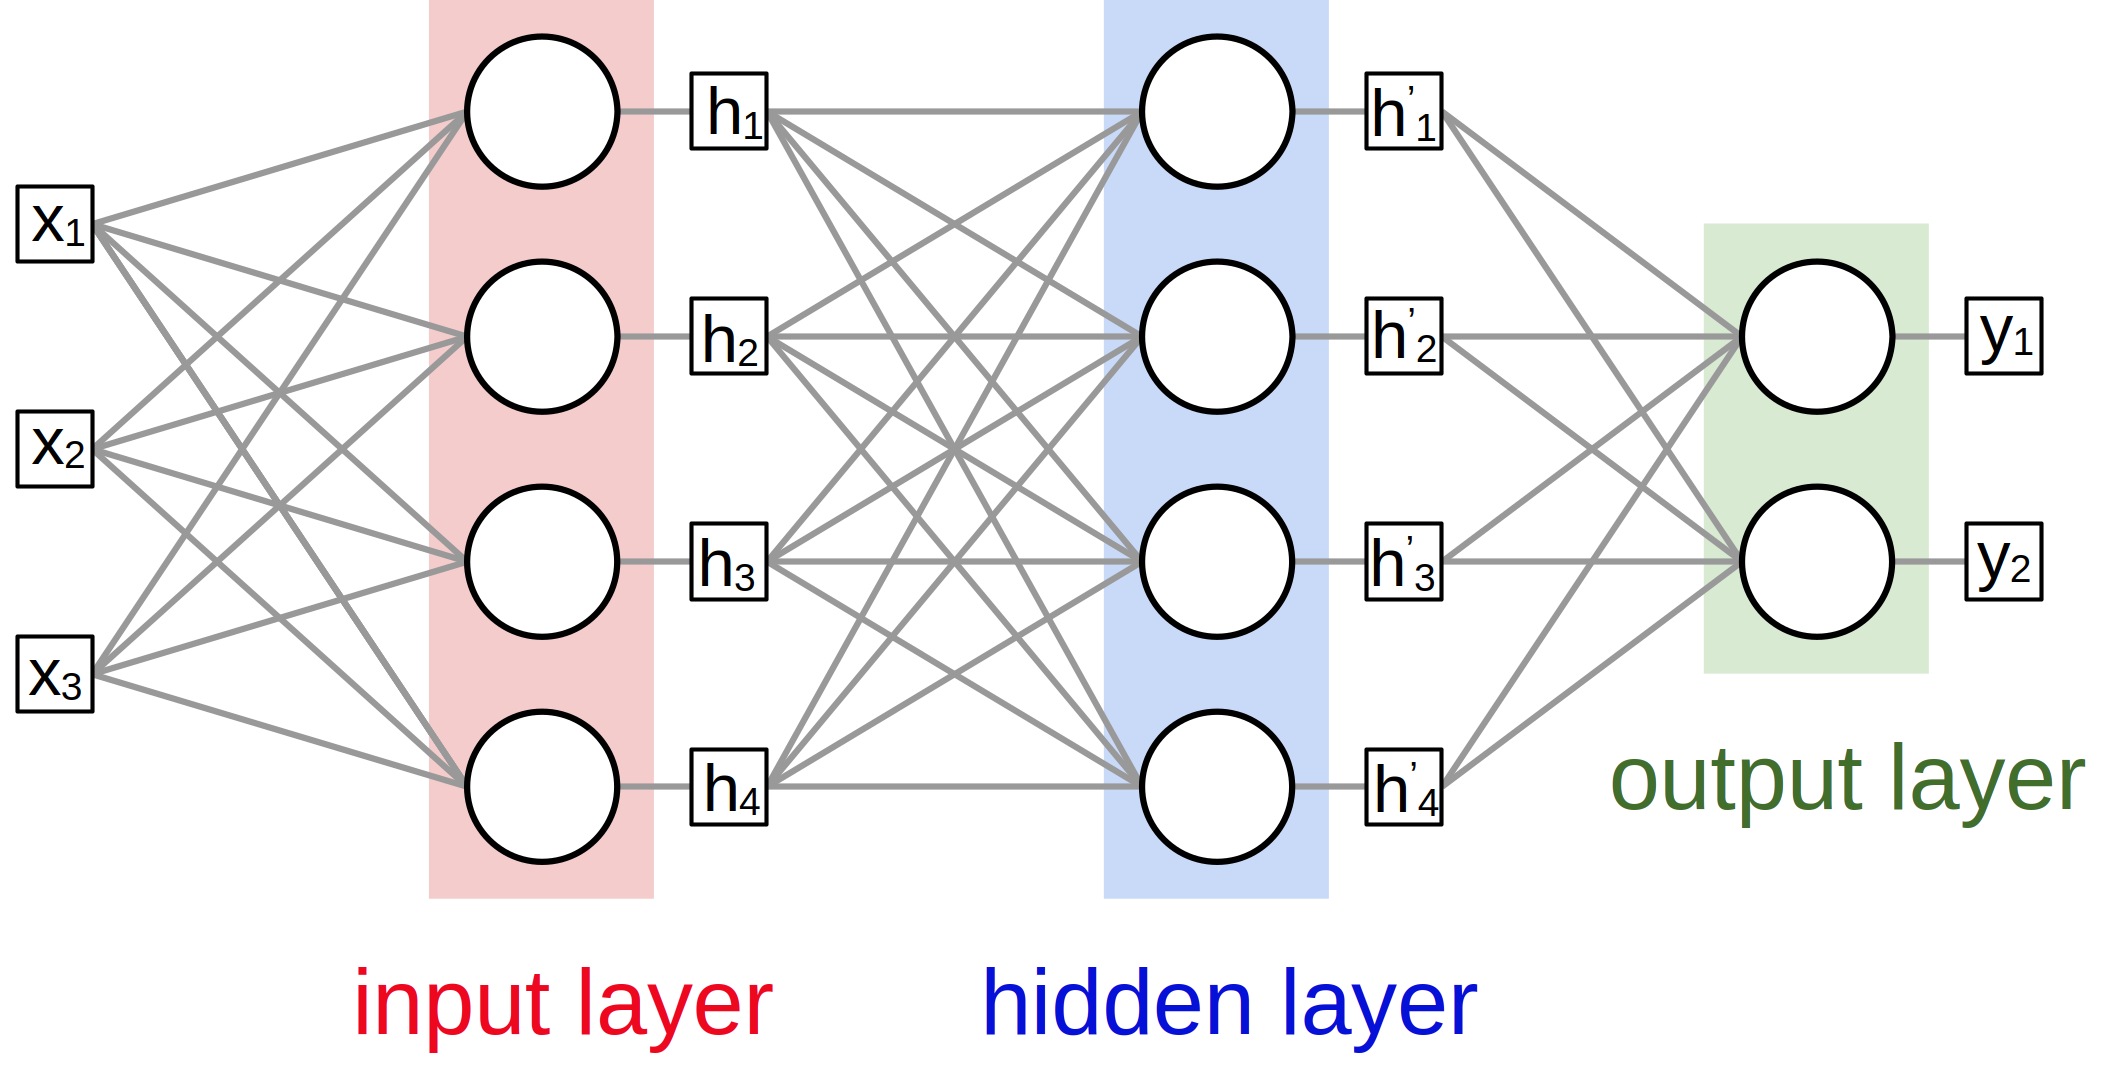
\includegraphics[width=11cm]{machine_learning/images/mlp}}
	\caption{A dense neural network with three layers. Each dot denotes an artificial neuron. The network takes an input $\vec{x}$ and projects it to $\vec{h}$, and then $\vec{h}'$, of hidden dimension four. The final output layer projects $\vec{h}'$ to $\vec{y}$.}
	\label{fig:machine_learning:mlp}
\end{figure}

% neurons arranged into fully connected layer 
% multiple layers form a neural network, a fully connected network (FCN) or dense network
% commonly this type of network is also called MLP, which is a misnomer, or FFN

These neurons can be arranged to form \emph{fully connected} or \emph{dense} layers. Such a layer takes $m$ inputs $\vec{x}$, and returns $n$ outputs $\vec{y}$, corresponding to the number of neurons. Each neuron is connected to all inputs, hence the name. Denoting the layer's weights $W_{m\times n}$ and the biases $\vec{b}$, this can be formalized as,
\begin{equation}
	\label{eq:machine_learning:dense_layer}
	\vec{y} = f(\vec{x}\,W_{m\times n} + \vec{b}).
\end{equation}
The term $\vec{x}\,W_{m\times n} + \vec{b}$ is conventionally called a \emph{linear projection} from the input dimension $m$ to the output dimension $n$, and it will be notated as $\text{Linear}_{m\rightarrow n}(\vec{x})$ in this thesis. The whole layer performs a non-linear projection then.

Stacking dense layers yields a fully connected or a dense neural network, which consists of one input layer, a number of hidden layers, and an output layer. Each layer's output corresponds to the next layer's input.  See a schematic in Fig.~\ref{fig:machine_learning:mlp}.
Stacked layers illustrate the importance of \emph{non-linear} activation functions, since without them, multiple layers would be equivalent to a single layer. 
Dense networks are commonly called multi-layer perceptrons (MLPs) or feed forward networks (FFNs).

% training
% dataset of labeled samples (supervised learning)
% training, validation, testing
% objective: minimize loss function L_L2 = sum (y_i-ŷ_i)²
% gradient descent 
% backpropagation
% batches

Having presented the basic form of a neural network, the question remains how its parameters should be chosen for the network to perform some specific task on a dataset. For a given dataset \emph{sample} $x$, the network makes a \emph{prediction} $\hat{y}$, which ideally corresponds to the true \emph{target} value $y$. In the context of GW searches, the input may be detector data, and the network predicts $1$ if that data contains a GW signal and $0$ otherwise. 

\begin{figure}
	\centering
	\makebox[\textwidth]{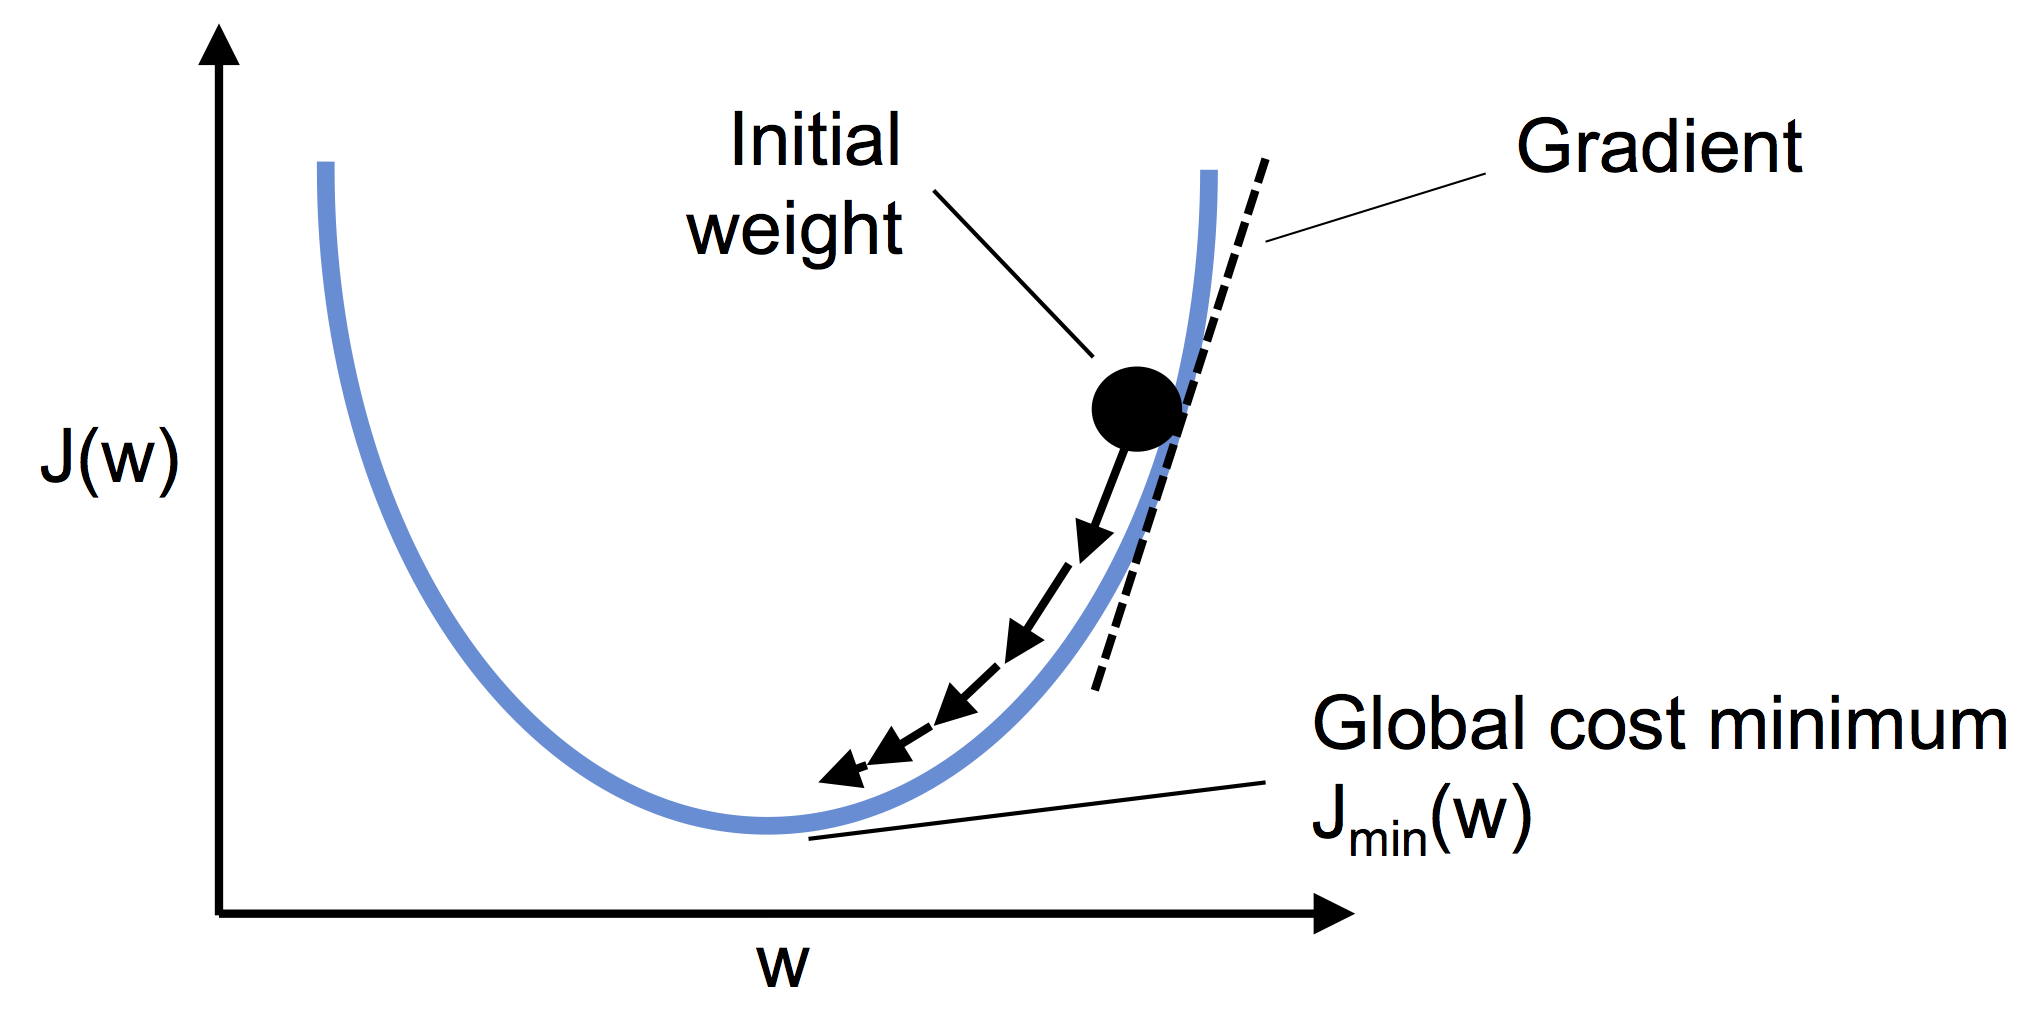
\includegraphics[width=10cm]{machine_learning/images/gradient_descent}}
	\caption{Gradient descent minimization of the loss $J$ with respect to the network parameters or weights $w$. This is a simplified sketch, where $w$ is one-dimensional. Contrast this with modern large language models with billions of parameters. Taken from \cite{raschka}.}
	\label{fig:machine_learning:gradient_descent}
\end{figure}

The process of optimizing a network's parameters is called \emph{training}. In particular, this thesis is concerned with \emph{supervised} learning, where this dataset is labeled, \emph{i.e.} the true values are known. In this case, the dataset is split into training, validation and testing subsets. The parameters are optimized by  minimizing a \emph{loss function} $\pazocal{L}$ over the training set, \emph{e.g.}, the mean-squared loss,
\begin{equation}
	\pazocal{L}_\text{MSE} = \frac{1}{N}\sum_{i=1}^{N}|\hat{y}(x_i, \vec{\theta}) - y_i|^2, 
\end{equation}
where $N$ is the number of training samples.
Notice that the total loss depends solely on the network parameters $\vec{\theta}$. Formally, the optimal parameters are given by,
\begin{equation}
	\vec{\theta}_\text{opt} = \argmin_{\vec{\theta}}
	\pazocal{L}(\vec{\theta}).
\end{equation}
Determining the minimum of $\pazocal{L}$ analytically is not possible once the model reaches a certain size. Instead, the parameters are initialized randomly and iteratively updated by calculating the gradient:
\begin{equation}
	\vec{\theta}' = \vec{\theta} - \eta\,\vec{\nabla}\pazocal{L}(\vec{\theta}),
\end{equation}
where $\eta$ denotes the \emph{learning rate}. This method is called \emph{gradient descent}. The parameters follow the slope of the loss hypersurface towards its minimum (see Fig.~\ref{fig:machine_learning:gradient_descent}). The loss gradient can be efficiently computed with \emph{backpropagation}, which is simply based on the chain rule.

In practice, it is often not feasible or even necessary to update the parameters based on the loss of the whole training dataset. Instead, small batches are chosen randomly, for which the parameters are updated subsequently. Once the whole dataset is exhausted, the process is repeated. One full iteration over the training dataset is called an \emph{epoch}.

% loss vs epochs -> learning curve -> overfit, underfit
% regularization
% dropout, lambda, decrease model size, increase number of samples

\section{Convolutional Neural Networks}

\begin{figure}
	\centering
	\makebox[\textwidth]{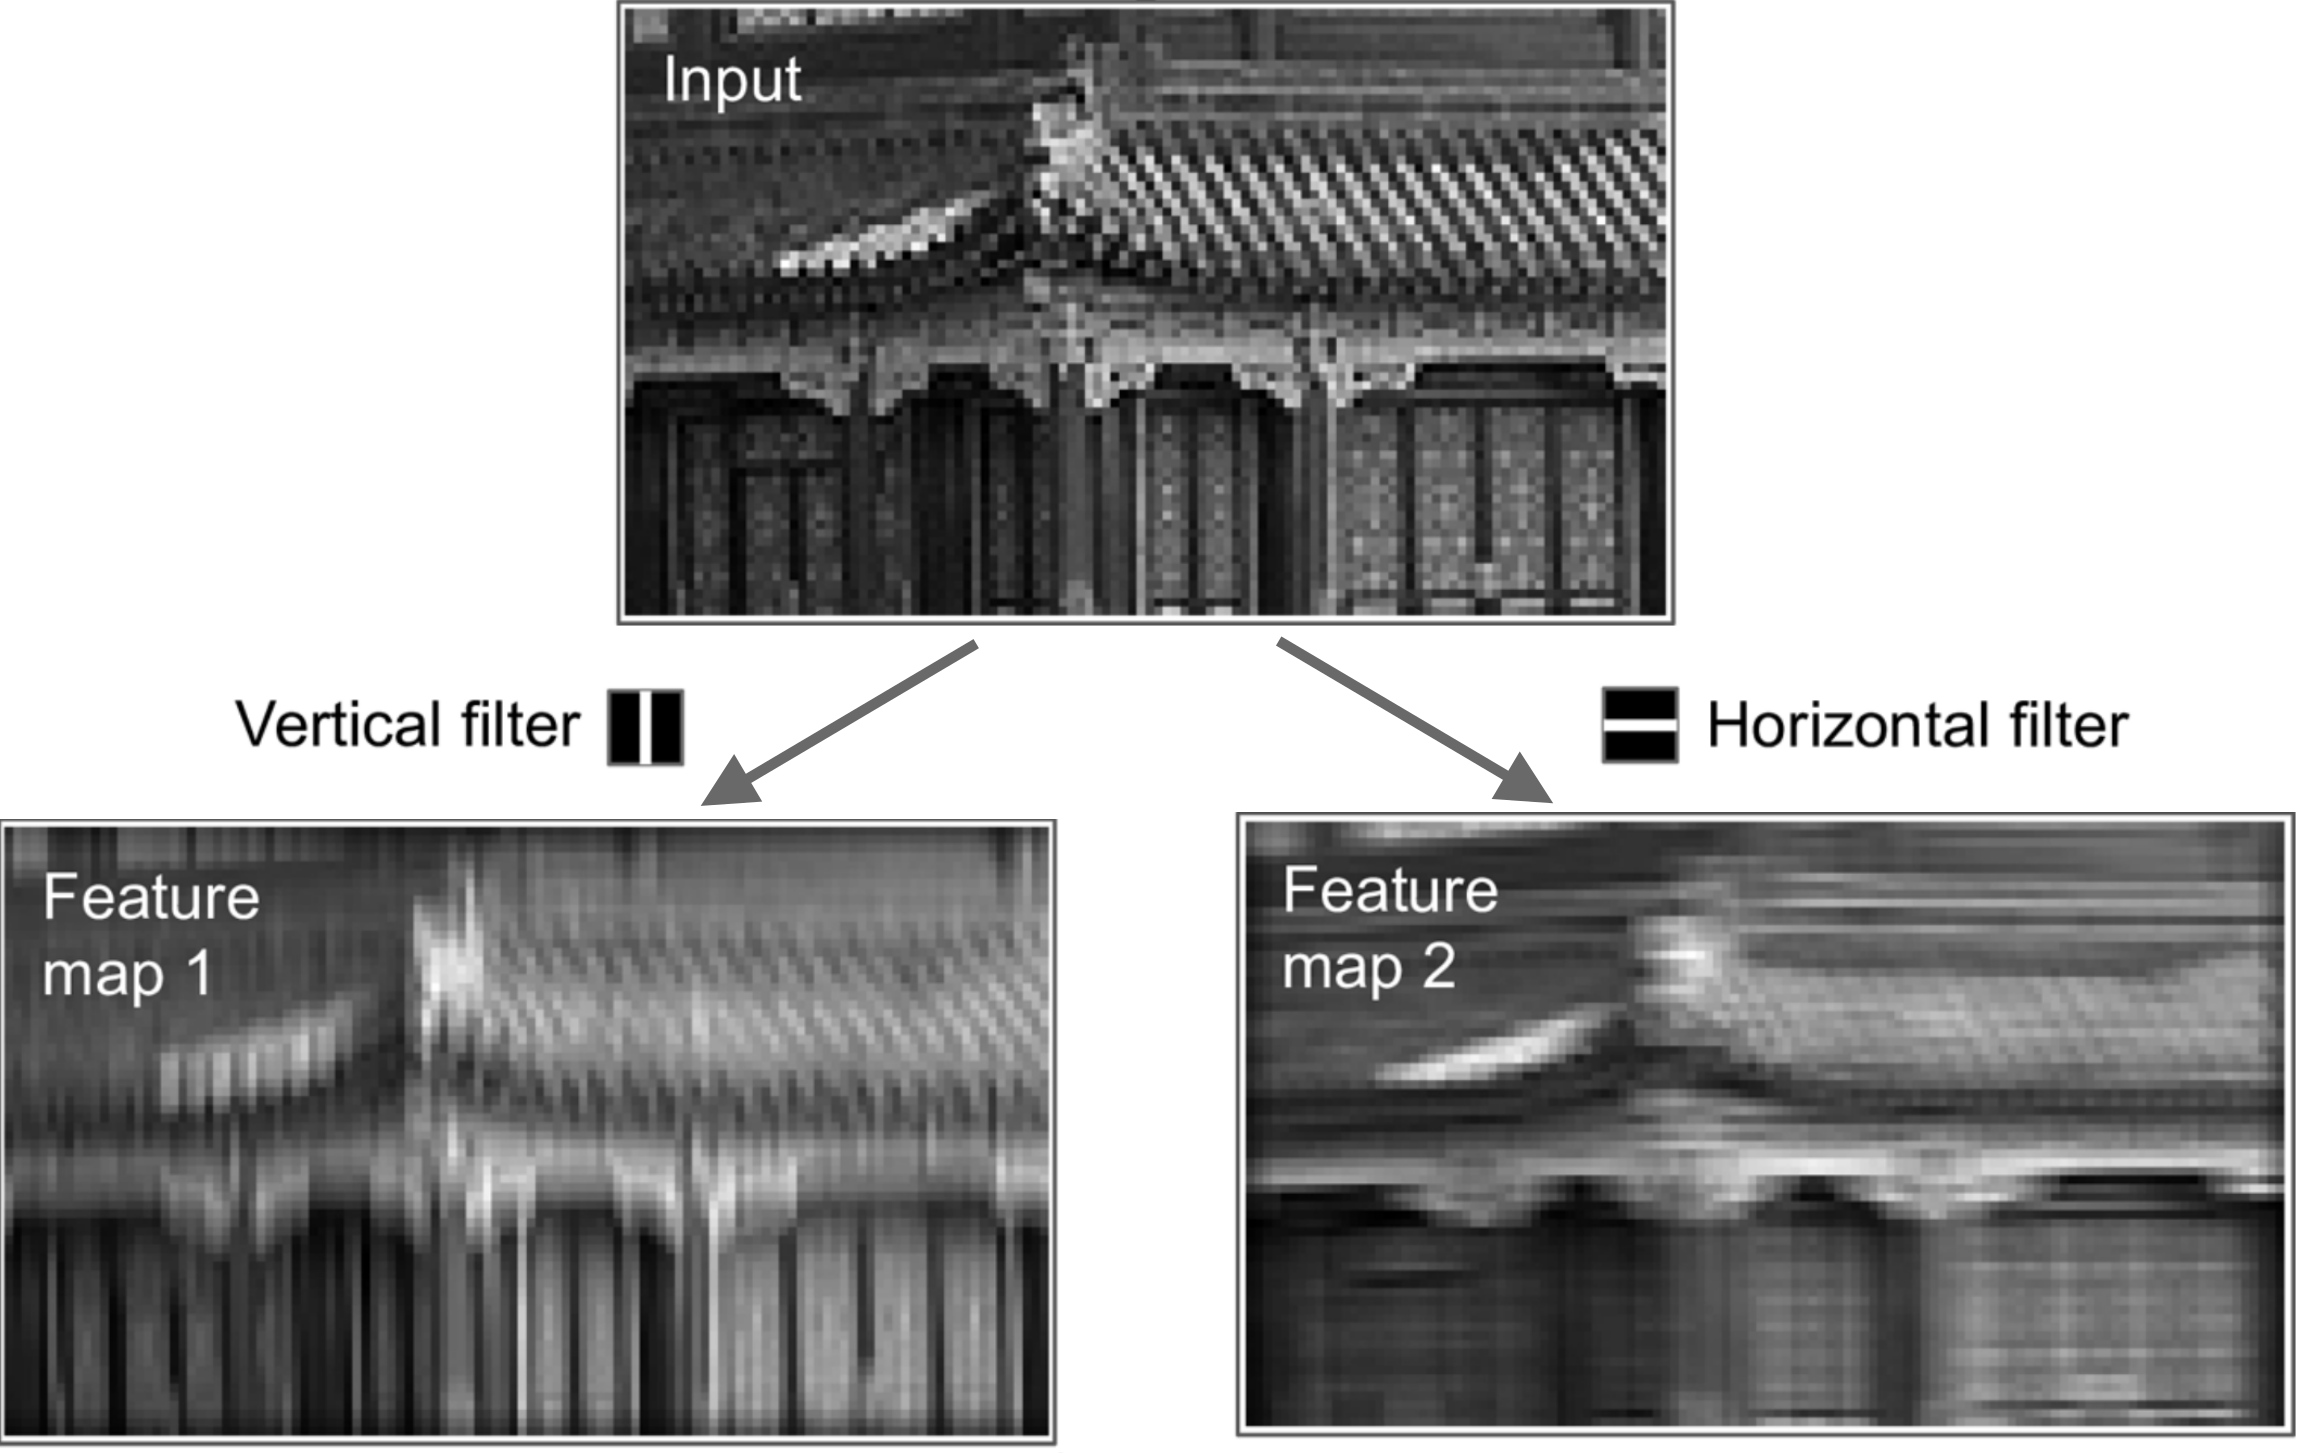
\includegraphics[width=11cm]{machine_learning/images/cnn/filter.png}}
	\caption{A \enquote{vertical} and a \enquote{horizontal} filter convolved over the image of a pagoda. In the feature map on the left, the vertical features stand out more. \emph{e.g.} the roof tiles and the columns. On the right they appear less bright and more blurry. Adapted from \cite{hands_on_ml}.}
	\label{fig:machine_learning:convolution}
\end{figure}

% Visual cortex -> conv operation (similarity to matched filtering) (explaing padding)

CNNs were first developed for image analysis and were inspired by the organization of neurons in the brain's visual cortex \cite{hands_on_ml}. In the visual cortex, neurons have a \enquote{small} receptive field, that is, they respond only to local regions of the visual field. The receptive fields of different neurons can overlap and together they cover the whole visual field. Moreover, neurons can specialize to recognize different local patterns, such as horizontal and vertical edges. 

CNNs model this behavior by convolving learnable filters, called \emph{kernels}, across the input. In practice, this operation is usually implemented as the cross-correlation between a kernel $k$ and an input $x$. In one dimension, this is given by
\begin{equation}
	(k\star x)(\tau) = \int_\mathbb{R}\mathrm{d}t\, k(t)\,x(t+\tau),
\end{equation}
and yields a measure of similarity as a function of $\tau$, the displacement of the input relative to the kernel. 
In discrete form, the convolution of a kernel $\vec{k}$ of size $N$ over an input $\vec{x}$ outputs a \emph{feature map} $\vec{y}$ with entries
\begin{equation}
	y_i = (\vec{k}\star\vec{x})_i = \sum_{j=0}^{N-1} k_j\,x_{i+j}.
\end{equation}
See Fig.~\ref{fig:machine_learning:convolution}, where two different kernels are applied to the same input image of a pagoda. One kernel extracts the input's vertical features, while the other extracts horizontal features.
The convolution operation gives neural networks the ability to extract features in a spatially invariant manner.
% TODO: more stuff about whats cool here

% explain CNN architecture:
% How do channels work
% Subsampling with pooling, stride

\begin{figure}
	\centering
	\makebox[\textwidth]{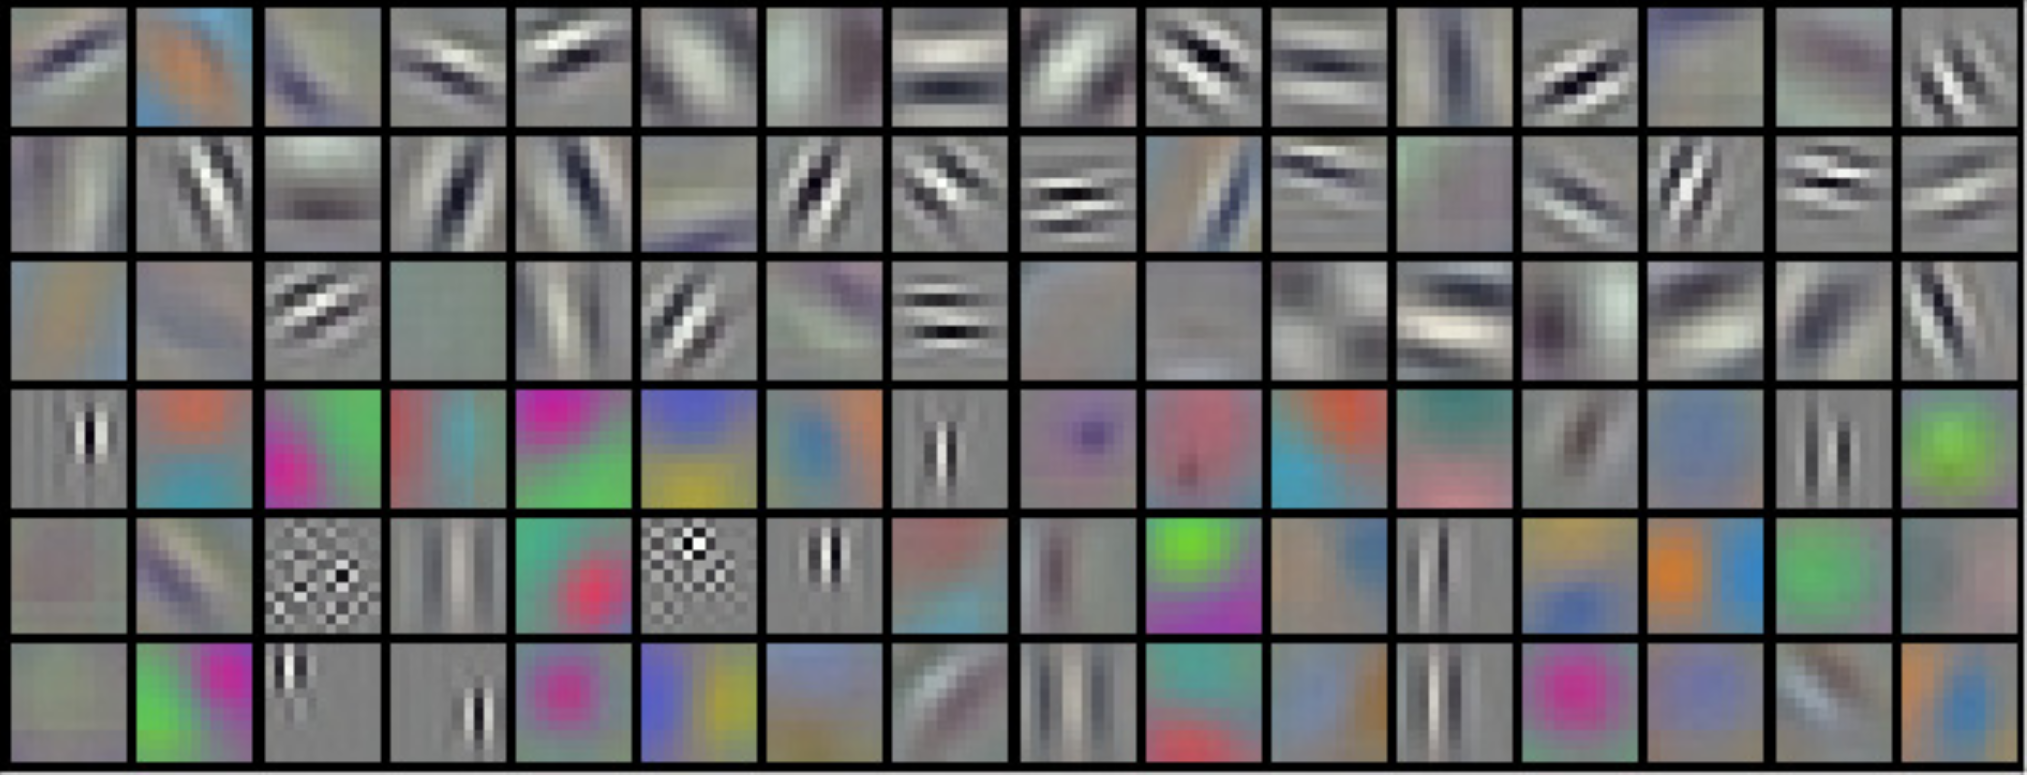
\includegraphics[width=10cm]{machine_learning/images/imagenet/kernels}}
	\caption{The initial convolutional layer's 96 kernels in AlexNet \cite{10.1145/3065386}. These are of shape $3\times11\times11$, and plotted as RGB images.}
	\label{fig:machine_learning:kernels}
\end{figure}

\begin{figure}
	\centering
	\makebox[\textwidth]{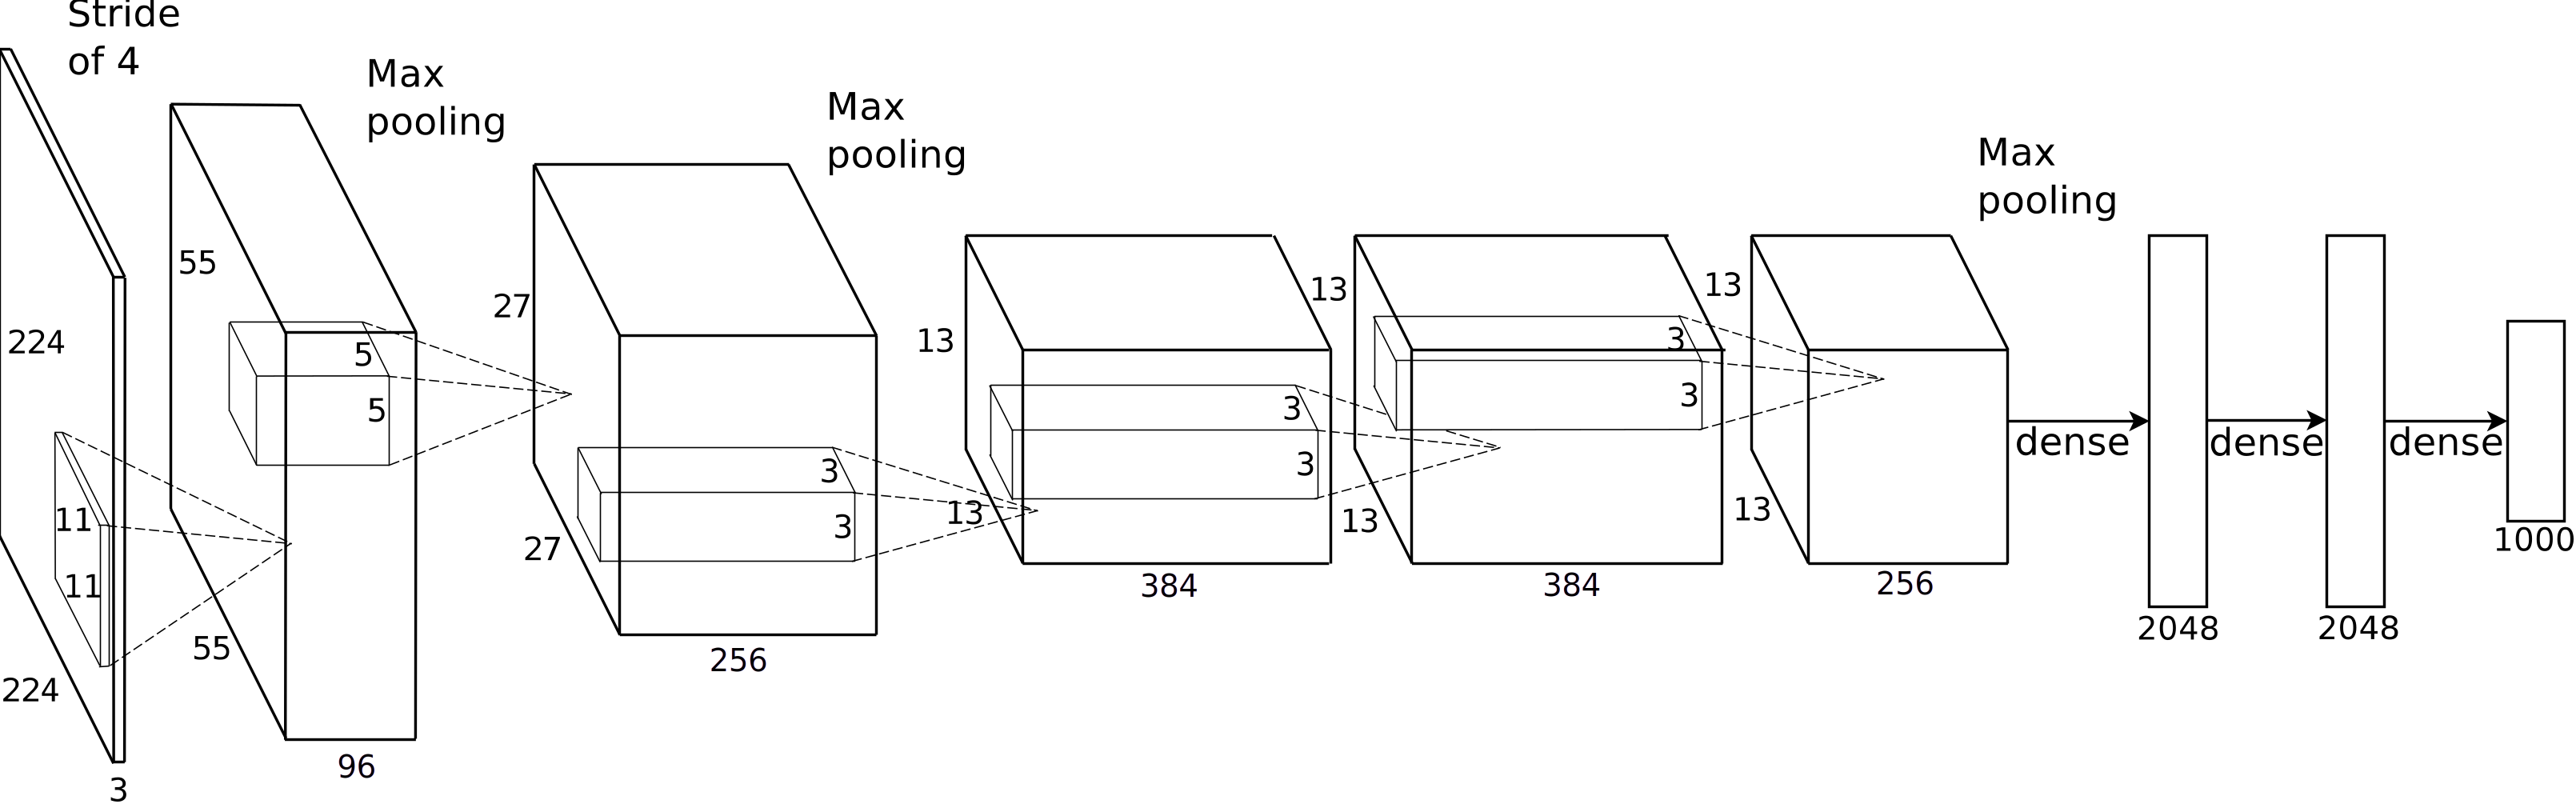
\includegraphics[width=17cm]{machine_learning/images/imagenet/Krizhevsky-2012.png}}
	\caption{AlexNet architecture \cite{10.1145/3065386}. Multiple stacked convolutional layers with ReLU and pooling in between, and a final dense network. The schematic has been adapted.}
	\label{fig:machine_learning:cnn}
\end{figure}

A full CNN architecture will consist of multiple stacked \emph{convolutional layers}. Each layer learns a number of kernels producing multiple feature maps, or \emph{channels}. One layer's output gets fed to the next layer.
This way, the complexity of the features that are extracted from the input gradually increases. 
The initial layers will learn low-level features, \emph{e.g.} vertical or horizontal edges, while the later layers can extract high-level features, \emph{e.g.} human faces or GW signals. See the learned low-level kernels of a 2D-CNN, AlexNet \cite{10.1145/3065386}, in Fig.~\ref{fig:machine_learning:kernels}. 

Generally, a 1D convolutional layer takes an input tensor $X$ of shape $C_\text{in} \times L$ and produces an output of shape $C_\text{out} \times L$. The sequence length is $L$, and $C_\text{in}$ and $C_\text{out}$ denote the number of input and output channels. The output of such a layer is then,
\begin{equation}
	\text{ConvLayer}_{C_\text{in}\rightarrow C_\text{out}}(X)
	= \concat_{i=0}^{C_\text{out}-1}\sum_{j=0}^{C_\text{in}-1} \vec{k}_{i,j}\star\vec{x}_j,
\end{equation}
with $\vec{k}_{i,j}$, the kernel corresponding to the $i$-th output channel and the $j$-th input channel.

Usually, the number of channels increases the deeper the CNN gets. To counteract the increased computational burden this introduces, CNNs often perform downsampling on the feature maps between each layer. This can be achieved by \emph{striding}, which disregards some of the feature map entries in an orderly fashion, \emph{e.g.} every second, which corresponds to a stride of two. Another way of downsampling is \emph{pooling}, where the feature map is subdivided into equal sized regions, and for each region only the maximum value or the mean value is extracted.

Most CNNs apply a number of convolutional layers, each followed by a ReLU non-linearity and downsampling. Without this non-linearity, multiple convolutional layers would be equivalent to a single layer, similar to stacked fully-connected layers. The final feature maps are usually flattened and fed to a fully-connected network to return an output of the desired size. See an example 2D-CNN in Fig.~\ref{fig:machine_learning:cnn}.

In GW signal detection, both two and one-dimensional CNNs are employed. In the former case, the network's input can be the strain spectrogram \cite{George_2018}, and in the latter case, it is the strain time series \cite{PhysRevD.100.063015}. Notice especially, the similarity of 1D-CNNs with matched filtering, which is based on \enquote{de-noising} the detector strain $s(t)$ with a filter function $K(t)$ via $\int\mathrm{d}tK(t)s(t)$ (see Eq.~\ref{eq:matched_filtering:filtered_strain}). In a way, the whole set of a CNN's kernel parameters can be thought of as a particularly efficient way of storing waveform templates.

\section{Transformers}
\label{sec:machine_learning:transformers}

% originally language processing, translation task
% also used in image or audio tasks
% based on attention

The Transformer \cite{NIPS2017_3f5ee243} was originally developed for natural language processing tasks (NLP), in particular for machine translation. 
Unlike CNNs, which rely on local receptive fields, Transformers model global dependencies through \emph{attention mechanisms}.
Transformers generalize well to other sequential data tasks, \emph{e.g.}\ image or audio related. A transformer-based model has proved successful in GW parameter estimation under ET conditions with signal overlap \cite{Papalini_2025}. This motivates the investigation of transformers for GW searches.

\subsection*{Attention Mechanism}

\begin{figure}
	\centering
	\makebox[\textwidth]{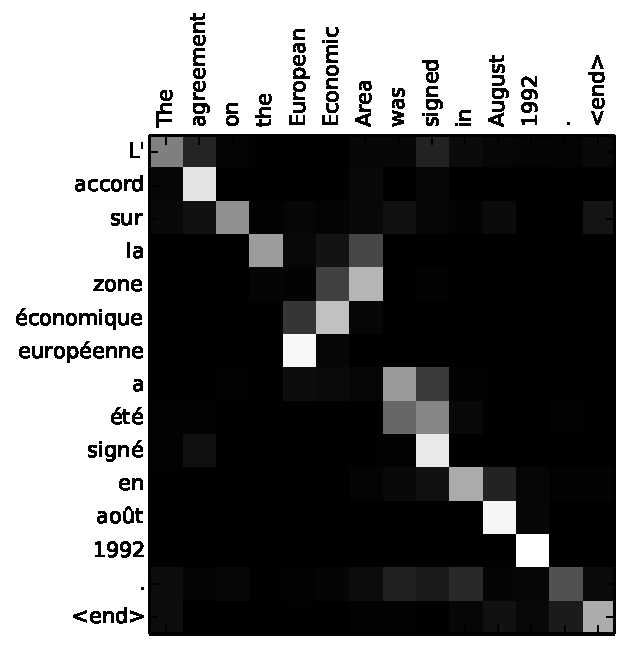
\includegraphics[width=8cm]{machine_learning/images/EEA}}
	\caption{Cross-attention matrix in an English-to-French translation model \cite{Bahdanau2014NeuralMT}. The English sentence is the source sequence, and the French translation the target sequence. Lighter colors mean higher values.}
	\label{fig:machine_learning:attn_matrix}
\end{figure}

The central component of the Transformer architecture is the attention mechanism, which builds on \cite{Bahdanau2014NeuralMT}. The mechanism takes two sequences as input. Each sequence comprises a number of tokens, which, \emph{e.g.}\ in NLP, can correspond to the words of a sentence. 
The two inputs are referred to as the \emph{source} sequence and the \emph{target} sequence. 
If both are the same, this is called \emph{self-attention}, and if they are different, it is \emph{cross-attention}. The attention mechanism relies on \emph{attention weights} to model the relationship between source and target sequence. These weights correspond to a $N_\text{tgt}\times N_\text{src}$ matrix. See an example in Fig.~\ref{fig:machine_learning:attn_matrix}, the attention matrix in an English-to-French translation model, capturing the relationship between  \enquote{area} in English and \enquote{zone} in French despite their different ordering in the two languages.

%\begin{figure}
%	\centering
%	\makebox[\textwidth]{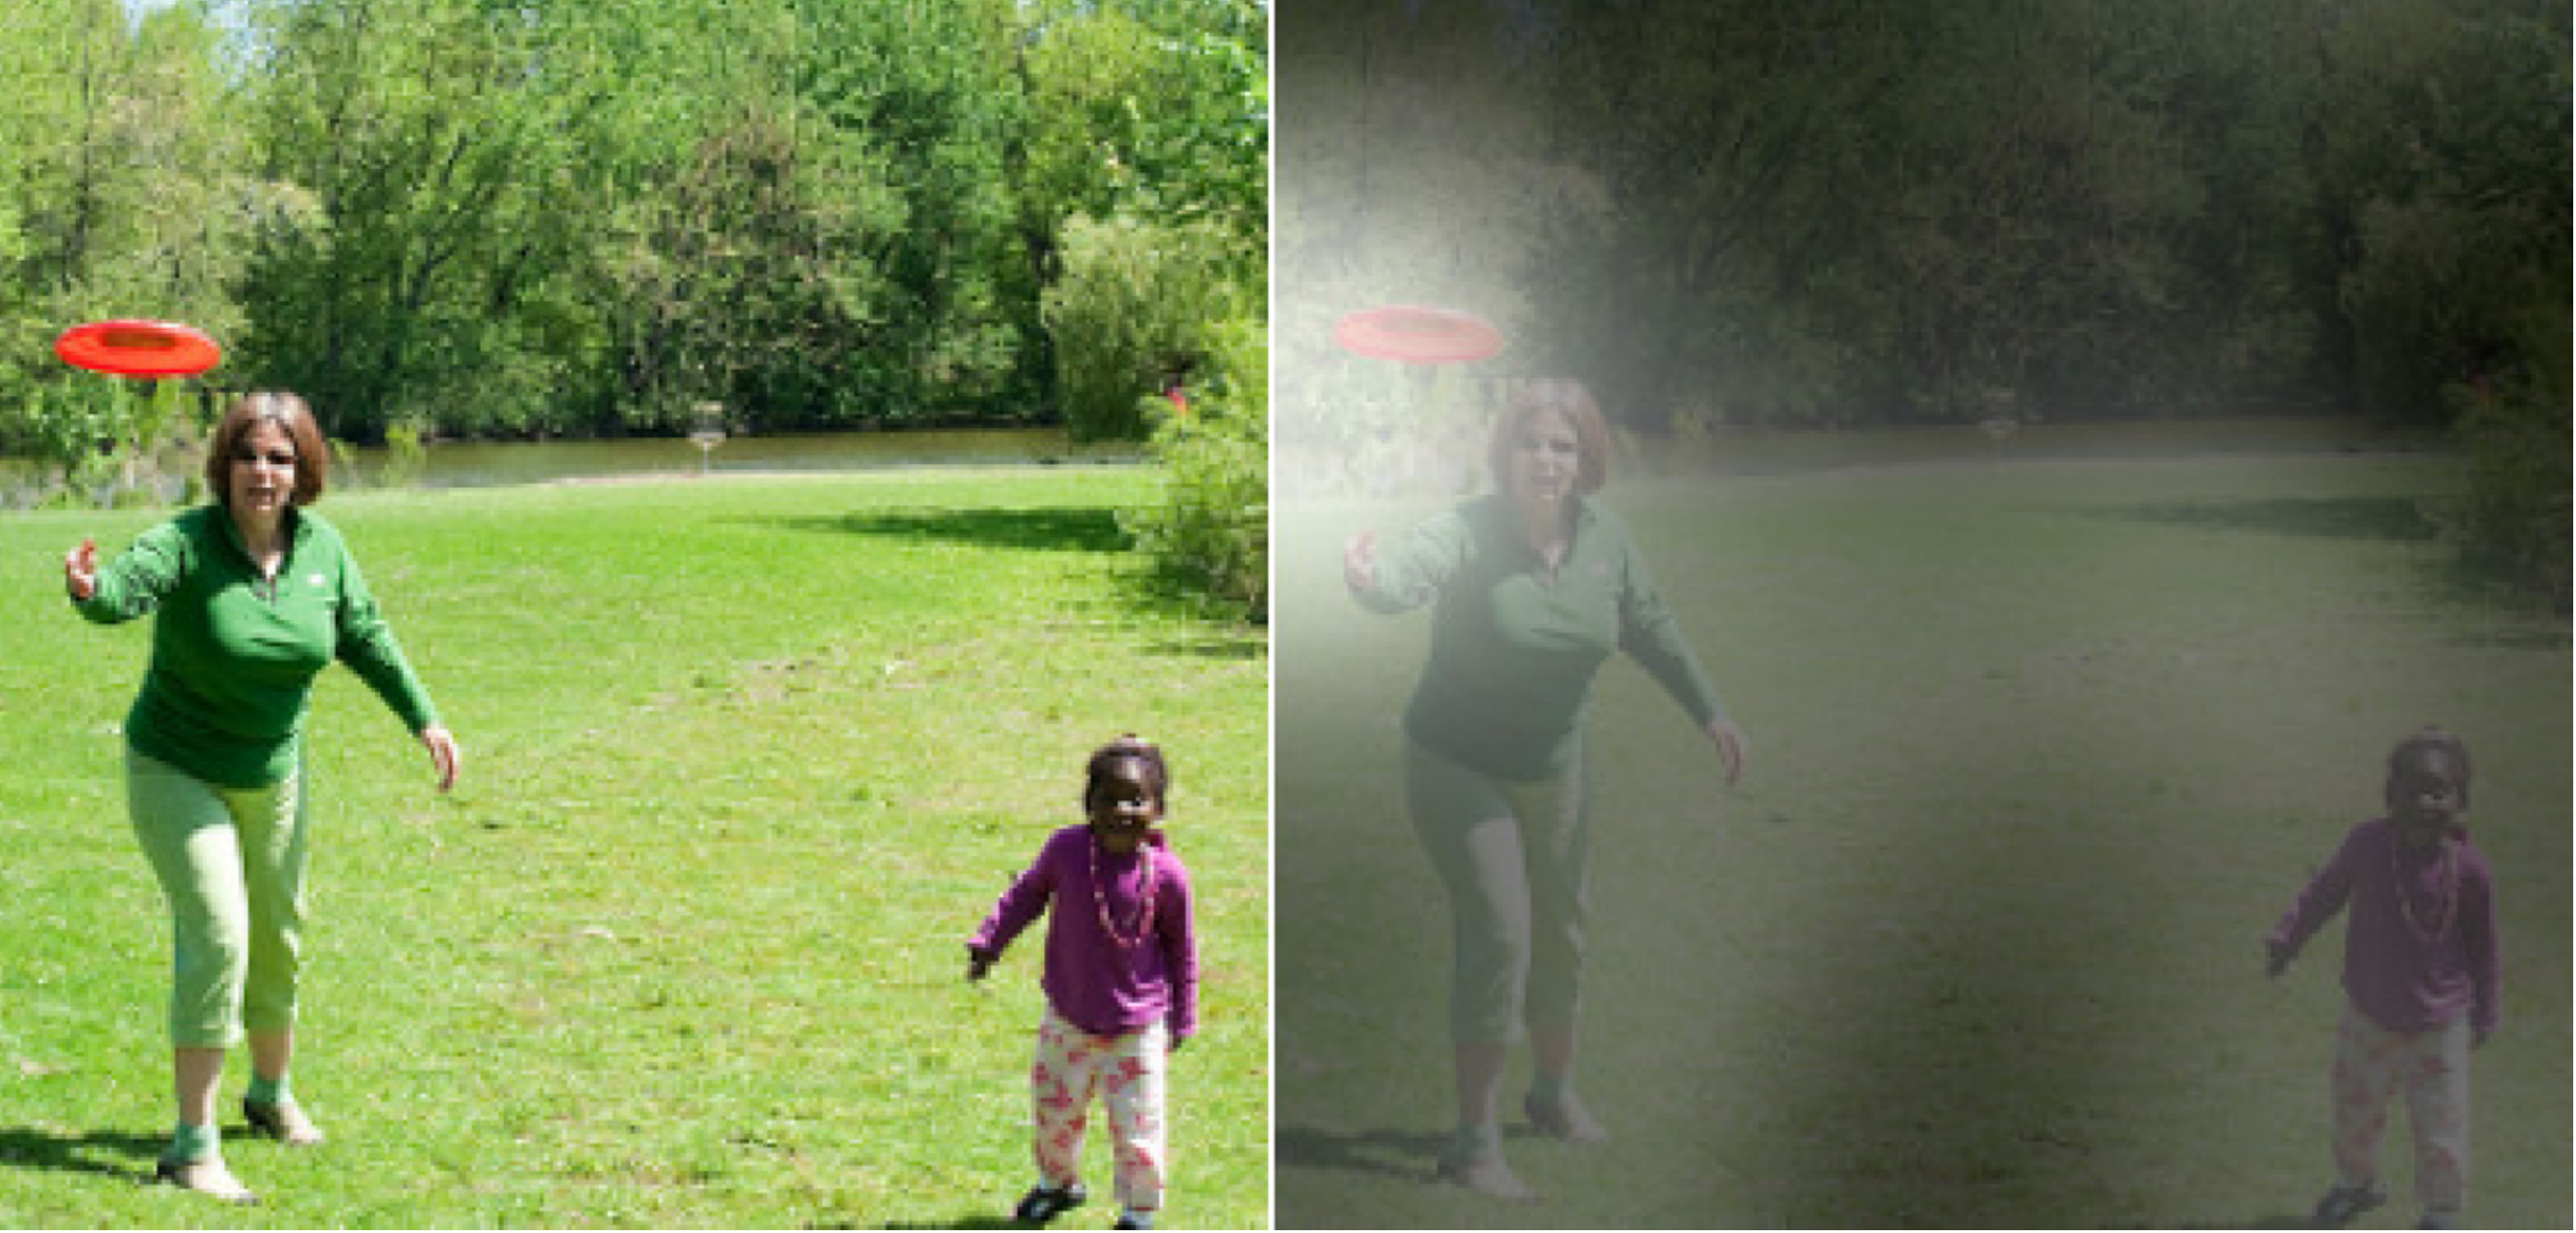
\includegraphics[width=13cm]{machine_learning/images/frisbee_attention}}
%	\caption{}
%	\label{fig:machine_learning:attention}
%\end{figure}

\subsection*{Scaled Dot-Product Attention}

In transformers, the attention mechanism is inspired by a search algorithm for a database of \emph{key}-\emph{value} pairs. The keys serve as identifiers and the values contain the actual data associated with them. The database is efficiently searched by matching a \emph{query} against the keys to retrieve the relevant values. 
For each query, the attention mechanism returns a weighted sum of all the values. The weights correspond to the similarity between the query and all keys, which is computed via their dot product.

This is implemented by linearly projecting the keys and values from the source sequence tokens, and the queries from the target sequence. The input tensors are denoted as $S_{N_\text{src}\times d_\text{src}}$ and $T_{N_\text{tgt}\times d_\text{tgt}}$, meaning source and target sequence respectively. Each sequence consists of a number of tokens $N$, which are vectors of size $d$. The queries, keys and values are then,
\begin{align}
	Q_{N_\text{tgt}\times d_\text{embed}} &= \text{Linear}_{d_\text{tgt} \rightarrow d_\text{embed}}(T) 
	\label{eq:machine_learning:q_proj} \\
	K_{N_\text{src}\times d_\text{embed}} &= \text{Linear}_{d_\text{src} \rightarrow d_\text{embed}}(S) 
	\label{eq:machine_learning:k_proj} \\
	V_{N_\text{src}\times d_\text{embed}} &= \text{Linear}_{d_\text{src} \rightarrow d_\text{embed}}(S)
	\label{eq:machine_learning:v_proj},
\end{align}
respectively, with the embedding dimension $d_\text{embed}$. (Notated like this, the linear projection only applies to the final tensor dimension, and its weights are shared across all other dimensions.)

From these, for each query vector $\vec{q}_i$, its weights $\vec{w}_i$ are computed as the dot product between that query vector and all keys:
\begin{equation}
	\vec{w}_i = \softmax\begin{pmatrix} 
		\vec{q}_i\cdot\vec{k}_0/\sqrt{d_\text{embed}} \\
		\vec{q}_i\cdot\vec{k}_1/\sqrt{d_\text{embed}} \\
		\vdots \\
		\vec{q}_i\cdot\vec{k}_{N_\text{src}-1}/\sqrt{d_\text{embed}}
	\end{pmatrix}.
\end{equation}
The dot product is scaled by the embedding dimension. \emph{Softmax} is applied to ensure that the weight vector sums to one. For an arbitrary vector $\vec{x}$ of size $N$ the softmax operation returns
\begin{equation}
	\softmax{\vec{x}} = \frac{1}{\sum_i \e^{x_i}} \begin{pmatrix}
		\e^{x_0} & \e^{x_1} & \dots & \e^{x_{N-1}}
	\end{pmatrix}^\intercal.
\end{equation}
The whole attention matrix has these weight vectors as its rows, \emph{i.e.},
\begin{equation}
	W_{N_\text{tgt}\times N_\text{src}} = \begin{pmatrix}
		\rule[0.5ex]{2.33em}{0.48pt}\;
		\vec{w}_0^\intercal 
		\,\rule[0.5ex]{2.33em}{0.48pt} \\
		\rule[0.5ex]{2.33em}{0.48pt}\; 
		\vec{w}_1^\intercal 
		\;\rule[0.5ex]{2.33em}{0.48pt} \\
		\vdots \\
		\rule[0.5ex]{1.5em}{0.48pt}\; 
		\vec{w}_{N_\text{tgt}-1}^\intercal 
		\;\rule[0.5ex]{1.5em}{0.48pt}
	\end{pmatrix}.
\end{equation}
Computing the attention weights as such is referred to as \emph{scaled dot-product attention}.

The attention mechanism will return a tensor of size $N_\text{tgt}\times d_\text{embed}$. To this end, the weight matrix and value tensor are multiplied. This yields a tensor, where each row is a weighted sum, $\sum_j w_{ij} \vec{v}_j$, corresponding to the $i$-th query. A final output linear projection is applied. The whole attention mechanism can be stated as,
\begin{equation}
	\label{eq:machine_learning:attn}
	\text{Attention}(Q, K, V) = \text{Linear}_{d_\text{embed} \rightarrow d_\text{embed}}(\softmax{\left(\frac{QK^\intercal}{\sqrt{d_\text{embed}}}\right)}\,V),
\end{equation}
with the attention matrix $W$ somewhat confusingly denoted as $\softmax{({QK^\intercal} / {\sqrt{d_\text{embed}}})}$, where softmax is applied along the final dimension.

Considering English-to-French machine-translation, the English sentence is the source sequence, while the target sequence somehow represents the French translation. (The correct translation is obviously not known beforehand. How the Transformer gains this representation will be covered later.) 
The projected values represent the English words in some abstract way, and the keys serve as labels for these values. Similarly, the query tokens are projected from the target sequence and encode what information is needed at each position. The French word corresponding to one of the queries is obtained by a weighted sum of all value tokens. The network learns to assign larger weights to the values most relevant to that position. A final linear layer projects this weighted sum of abstract English word representations into a French word representation.

\begin{figure}
	\centering
	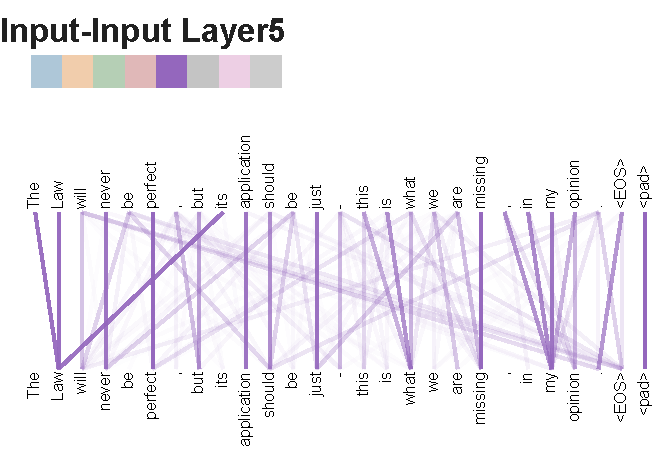
\includegraphics[
	width=10cm,
	trim=0cm 0cm 0cm 2cm,
	clip,
	angle=-90
	]{machine_learning/images/anaphora_resolution_new}
	\hspace{0.5em}
	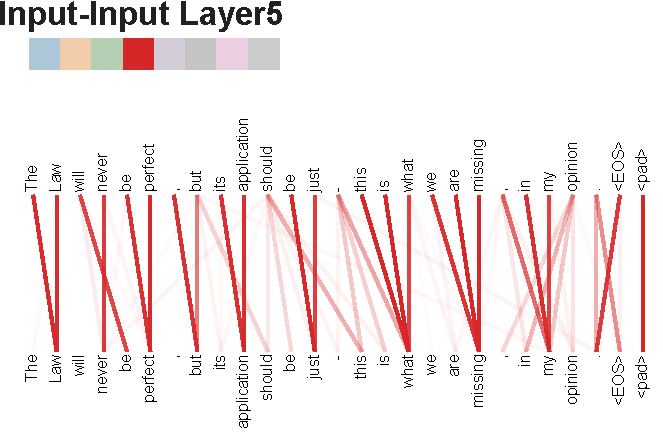
\includegraphics[
	width=10cm,
	trim=0cm 0cm 0cm 2cm,
	clip,
	angle=-90
	]{machine_learning/images/attending_to_head2_new}
	\hspace{0.5em}
	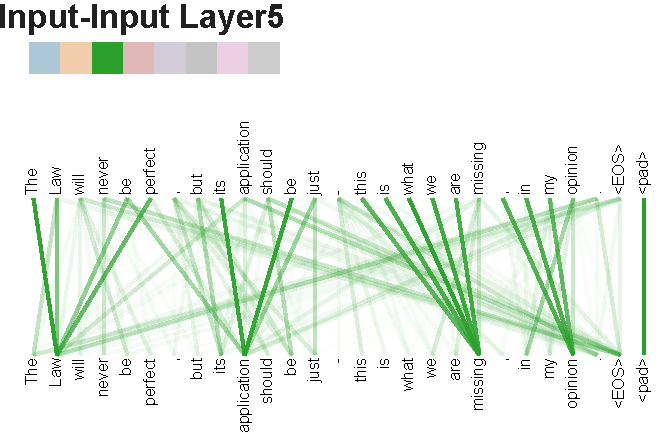
\includegraphics[
	width=10cm,
	trim=0cm 0cm 0cm 2cm,
	clip,
	angle=-90
	]{machine_learning/images/attending_to_head_new}
	\caption{Self-attention weights of different heads in the original Transformer \cite{NIPS2017_3f5ee243}.}
	\label{fig:machine_learning:mha}
\end{figure}

\subsection*{Multi-Head Attention}

Transformers develop the attention mechanism further to include multiple \emph{heads}. Each head learns its own query, key and value projections, and performs the attention mechanism independently of other heads. The idea is that each head can learn to perform different tasks (see Fig.~\ref{fig:machine_learning:mha}). This is called \emph{multi-head attention} (MHA).

In practice, to not introduce additional computational strain, the embedding dimension inside each head is reduced. This is usually implemented by keeping the original projections (Eqs.~\ref{eq:machine_learning:q_proj}, \ref{eq:machine_learning:k_proj}, \ref{eq:machine_learning:v_proj}), and splitting each tensor into $N_\text{heads}$ heads along the embedding dimension to yield tensors $Q_i$ of size $N_\text{tgt}\times d_\text{embed}/N_\text{heads}$ and $K_i$, $V_i$ of shape $N_\text{src}\times d_\text{embed}/N_\text{heads}$. For this to work, $d_\text{embed}$ has to be divisible by the total number of heads. The output of all heads is concatenated along their final dimension, and a linear projection is applied: 
\begin{equation}
	\text{MHA}(Q, K, V) 
	= \text{Linear}_{d_\text{embed} \rightarrow d_\text{embed}}
	{(\concat_{i=0}^{N_\text{heads}-1}
	{(\softmax{\left(\frac{Q_iK_i^\intercal}{\sqrt{{d_\text{embed}}/{N_\text{heads}}}}\right)}V_i)})}.
\end{equation}
Notice that for a single head, this is equivalent to Eq.~\ref{eq:machine_learning:attn}.

\subsection*{Model Architecture}

\begin{figure}
	\centering
	\begin{minipage}[t]{7cm}
		\centering
		\makebox[\textwidth]{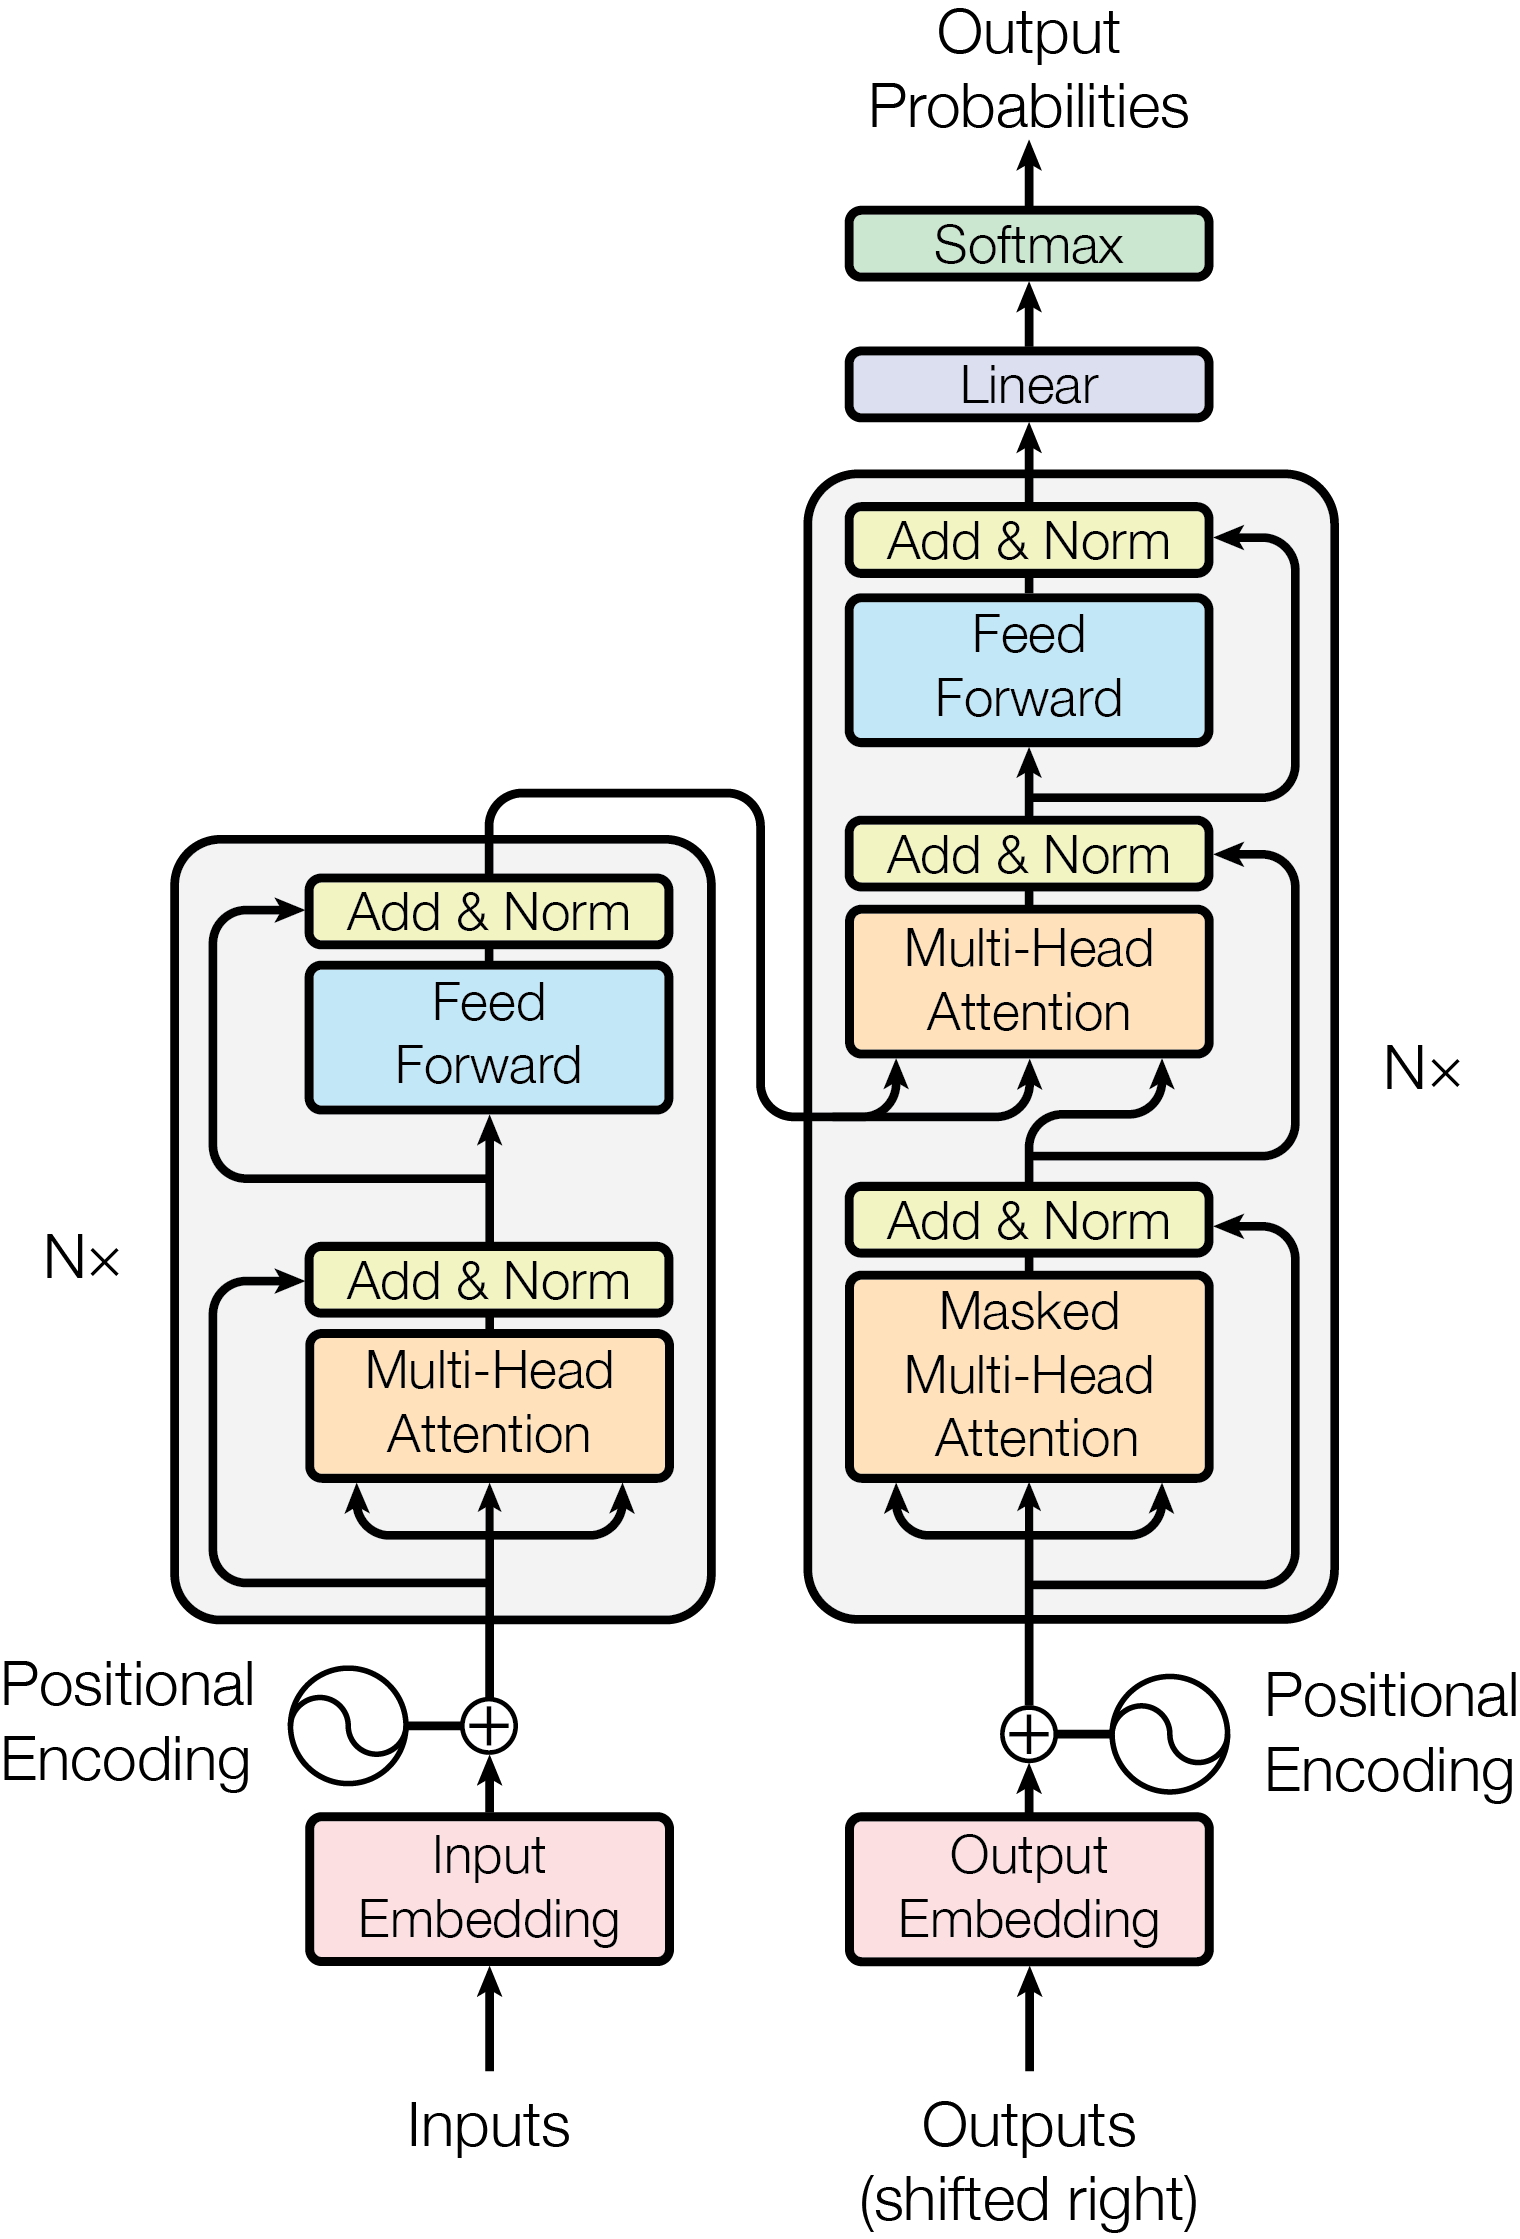
\includegraphics[width=7cm]{machine_learning/images/transformer_architecture}}
		\captionof{figure}{The original Transformer architecture \cite{NIPS2017_3f5ee243}.}
		\label{fig:machine_learning:transformer}
	\end{minipage}%
	\begin{minipage}[t]{9cm}
		\centering
		\makebox[\textwidth]{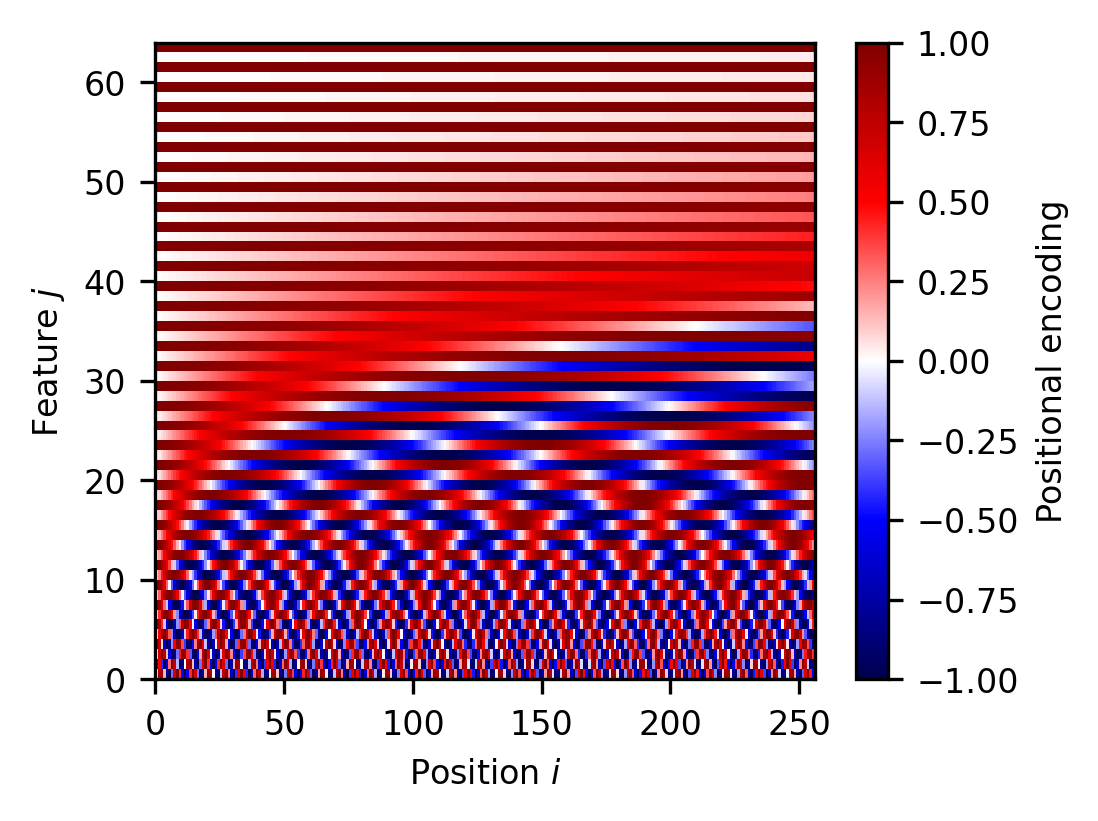
\includegraphics[width=9cm]{machine_learning/images/transformer/positional_encoding}}
		\captionof{figure}{Sinusoidal positional encodings.}
		\label{fig:machine_learning:pos_enc}
	\end{minipage}
\end{figure}

The Transformer follows an encoder--decoder architecture (see Fig.~\ref{fig:machine_learning:transformer}). The encoder processes the input sequence into an abstract representation, and the decoder  generates the output sequence from this representation. 
The decoder predicts the output sequence in an autoregressive manner, that is, token by token, starting with a beginning-of-sentence token. This makes sense for machine translation, while for other tasks the decoder can also be adapted to make predictions in parallel instead.
Modern transformer models often employ only the encoder or decoder.

Both the encoder and decoder are composed of identical stacked layers, where each layer's output is the next one's input. These layers comprise sub-layers of multi-head attention and dense networks, \emph{i.e.}\ feed-forward networks (FFNs). 

The encoder layers apply two sub-layers, self-attention followed by an FFN. The decoder layers apply three sub-layers instead: \emph{masked} self-attention, followed by cross-attention and an FFN. Masking the self-attention sub-layer ensures that the decoder can only attend to previously predicted tokens. Transformer models, which predict tokens in parallel, omit this masking. The cross-attention's source sequence is the encoder output and the target sequence is obtained from the previous sub-layer.

% residual layers
% layernorm
The architecture makes use of \emph{residual connections} for all  sub-layers, where the input is added to the output, \emph{i.e.}, $x + \text{SubLayer}(x)$. This works, since both these sub-layers return a tensor of the same dimension as the input. The FFN is,
\begin{equation}
	\text{FFN}(x) = \text{Dropout}(\text{Linear}_{d_\text{ff} \rightarrow d_\text{embed}}(\text{GELU}(\text{Linear}_{d_\text{embed} \rightarrow d_\text{ff}}(x)))),
\end{equation}
with hidden dimension $d_\text{ff}$, and a Gaussian error linear unit (GELU) activation~\cite{hendrycks2017bridging}.
Dropout~\cite{JMLR:v15:srivastava14a} is a regularization technique, which prevents networks from overfitting by randomly zeroing out elements of the given tensor. Dropout is not applied during inference.
In the original architecture, the residual connection is followed by a \emph{layer normalization}~\cite{ba2016layernormalization} to standardize the output along the embedding dimension.
This is called \emph{post}-layer normalization. To ease training, modern implementations often employ \emph{pre}-layer normalization, so $x + \text{SubLayer}(\text{LayerNorm}(x))$ instead. 

% positional encoding
Unlike in CNNs, the sequential nature of the data is not baked into the Transformer architecture itself. Thus, \emph{positional encodings} are added to encoder and decoder input tokens. The original Transformer makes use of so-called fixed sinusoidal encodings. For a token position $i<N_\text{tokens}$ and a feature $j<d_\text{embed}$, this is:  
\begin{equation}
	P(i,j) = \begin{cases}
		\sin{({i}/{N^{\frac{j}{d_\text{embed}}}})} & \text{if $j$ even,} \\
		\cos{({i}/{N^{\frac{j-1}{d_\text{embed}}}})} & \text{if $j$ odd,}
	\end{cases}
\end{equation}
where $N=\SI{E+4}{\nothing}$. See the encodings of $256$ tokens with an embedding dimension of $64$ plotted in Fig.~\ref{fig:machine_learning:pos_enc}.

%\begin{align}
%\begin{split}
%	n_1 &= \text{LayerNorm}(x) \\
%	y &= n_1 + \text{MHA}(n_1, n_1) \\
%	n_2 &= \text{LayerNorm}(y) \\
%	z &= n_2 + \text{FFN}(n_2)
%\end{split}
%\end{align}
%
%\begin{align}
%\begin{split}
%	n_1 &= \text{LayerNorm}(t) \\
%	x &= n_1 + \text{MHA}(n_1, n_1) \\
%	n_2 &= \text{LayerNorm}(x) \\
%	y &= n_2 + \text{MHA}(c, n_2) \\
%	n_3 &= \text{LayerNorm}(y) \\
%	z &= n_3 + \text{FFN}(n_3)
%\end{split}
%\end{align}



\chapter{Data Simulation}
\label{sec:data_simulation}
Since the Einstein Telescope is currently still in its planning stages, no real detector data exist, with which neural networks can be trained and tested. 
Thus, a considerable amount of this thesis' work has been spent on simulating gravitational wave signals, and the corresponding detector response under realistic noise conditions. 
In the context of machine learning, such simulated data is commonly referred to as \emph{synthetic} data.

This chapter provides a detailed description of the simulation of detector noise and GW signals, as well as the construction of samples to form datasets.
Most of the utilities required for these simulations are provided by the PyCBC software package \cite{alex_nitz_2023_10013996}, and the hardware was provided by the PALMA II HPC of the University of Münster.

\section{Detector Noise}
\label{sec:data_simulation:noise}
\begin{figure}
	\centering
	\makebox[\textwidth]{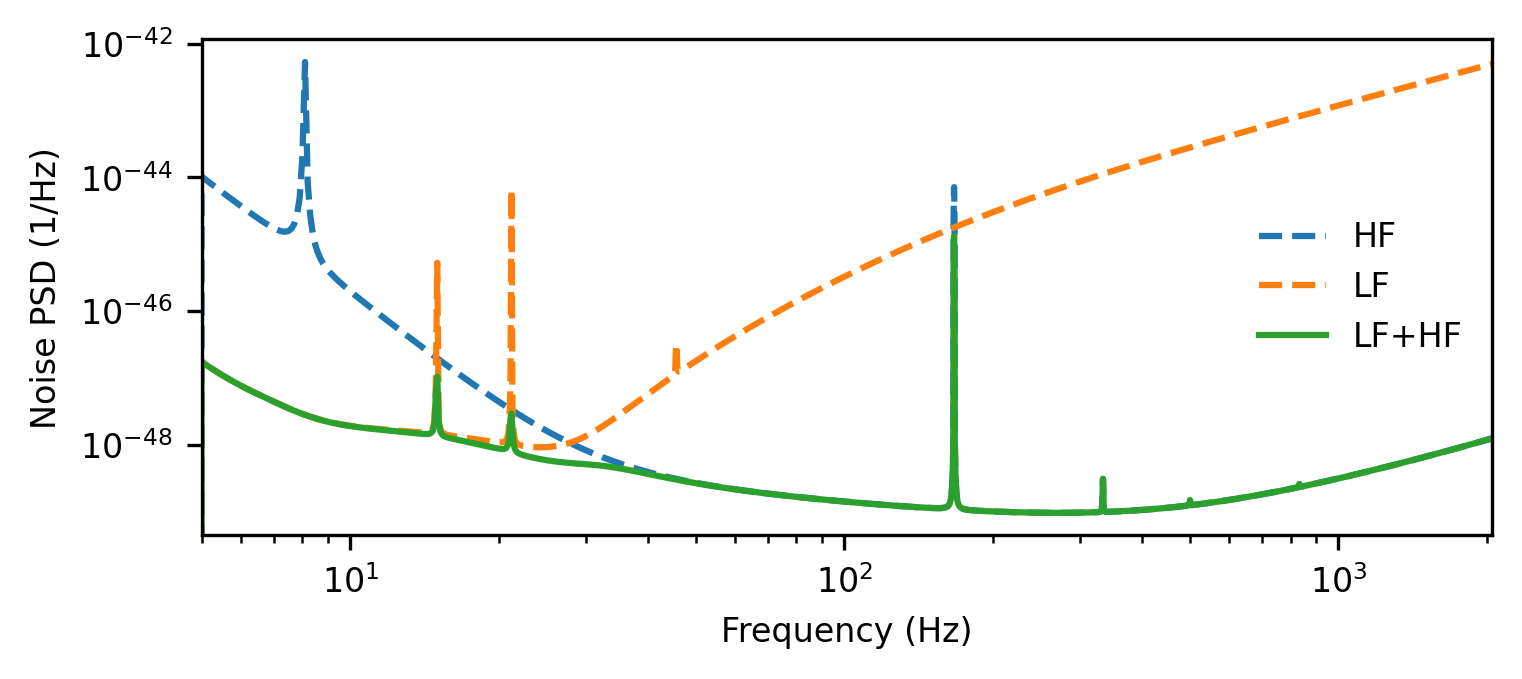
\includegraphics[width=13cm]{data_simulation/images/ET-0304B-22/18213_ET10km.png}}
	\caption{The ET noise PSD of the LF and HF interferometers, and of their combination (LF+HF), which is the PSD employed in this work. The PSDs are plotted from \SI{4}{\hertz} to \SI{2048}{\hertz}, corresponding to the simulation upper and lower frequency range. Data taken from \cite{ET-0304B-22}.}
	\label{fig:data_simulation:noise_psd}
\end{figure}

This thesis assumes the detector noise to be \emph{Gaussian}, meaning it has amplitudes, which are normally distributed. The noise is then fully characterized by the noise power spectral density (PSD). See Ch.~\ref{sec:matched_filtering} for further information. This thesis employs the sensitivity of ET according to the latest design report \cite{ET-0007C-20} in a triangular configuration with \SI{10}{\kilo\meter}-long arms (see Ch.~\ref{sec:einstein_telescope}).
The corresponding PSD data are taken from \cite{ET-0304B-22}, which provides the noise PSDs for the LF and HF interferometers in the frequency range from \SI{1}{\hertz} to \SI{10}{\kilo\hertz}, as well as for their
combined sensitivity (LF+HF).
The combined PSD is obtained through, 
\begin{equation}
	\frac{1}{S_n^\text{LF+HF}(f)} = \frac{1}{S_n^\text{LF}(f)} + \frac{1}{S_n^\text{HF}(f)}.
\end{equation} 
The corresponding PSD curves are shown in Fig.~\ref{fig:data_simulation:noise_psd}.
In this work, the intricacies of the xylophone configuration, where each detector consists of two nested interferometers, are ignored. Instead, ET is treated as three interferometers in a triangular configuration, assuming the ET LF+HF noise PSD for each. 

Such noise is called \emph{colored}, because its power spectrum is \emph{not} constant over the whole frequency regime (in contrast to \emph{white} noise with a flat power spectrum), and \emph{stationary} because the power spectrum stays constant with respect to time. Notice that for currently operating GW interferometers such as LIGO and Virgo their noise is typically non-stationary. This is due to slow drifts in the PSD over minutes or hours and because of short-duration transient noise events called \emph{glitches} \cite{Abbott_2020}. Regardless, in this work the detectors' noise is assumed to be stationary, since it is not entirely clear if and how exactly non-stationarity might arise.

In the proposed ET xylophone configuration, some of the interferometers' test masses will be located less than a few \SI{100}{\meter} apart, which is why a non-negligible correlation is expected among the noise of the detectors in the form of seismic noise, especially in the low-frequency regime up to \SI{\sim40}{\hertz} \cite{PhysRevD.109.102002}. Currently, there is no routine implemented in PyCBC for the simulation of correlated noise. Instead, this is done from scratch following the approach in \cite{PhysRevD.110.104060}. The algorithm will be presented by first describing how uncorrelated noise is simulated from a given power spectrum, and then showing how this procedure is adapted in the case of correlated noise.

\subsection*{Uncorrelated Noise}

Consider a noise time-series $n = (n(t_0), n(t_1), \dots)$ that is to be simulated for one detector with a PSD $S_n = (S_n(f_0), S_n(f_1), \dots)$. The discrete Fourier transform of that time-series $\tilde{n} = (\tilde{n}(f_0), \tilde{n}(f_1), \dots)$ should then satisfy,
\begin{equation}
	\label{eq:data_simulation:psd_relationship}
	\frac{1}{2}S_n(f) = \Delta f\bigl\langle|\tilde{n}(f)|^2\bigr\rangle, 
\end{equation}
where $\Delta f$ is the frequency resolution. This follows from the PSD definition (Eq.~\ref{eq:matched_filtering:PSD_definition}), as evaluated over a constant observation time $T$, in discrete form. Requiring the noise to be Gaussian, motivates an ansatz of the form,
\begin{equation}
	\label{eq:data_simulation:uncorrelated_noise_dft_ansatz}
	\tilde{n}(f) = a (x + iy), 
\end{equation}
where $x$ and $y$ are drawn from a normal distribution with zero mean and unit variance, $x, y \sim \pazocal{N}(\mu=0, \sigma^2=1)$, and where $a$ is some arbitrary prefactor. Since the expectation value of a squared normal random variate is one, $\bigl\langle|\tilde{n}(f)|^2\bigr\rangle = a^2 (\langle x^2\rangle + \langle y^2\rangle)$ simplifies to $2 a^2$, and thus with Eq.~\ref{eq:data_simulation:psd_relationship},
\begin{equation}
	\label{eq:data_simulation:prefactor}
	a = \frac{1}{2}\sqrt{\frac{S_n(f)}{\Delta\!f}}.
\end{equation}
That is, the discrete Fourier transform of the noise has a uniformly random phase and a magnitude, which is, on average, proportional to the square root of the noise PSD. Finally, $n$ can be computed as the inverse discrete Fourier transform of $\tilde{n}$.

\subsection*{Correlated Noise}

\begin{figure}
	\centering
	\makebox[\textwidth]{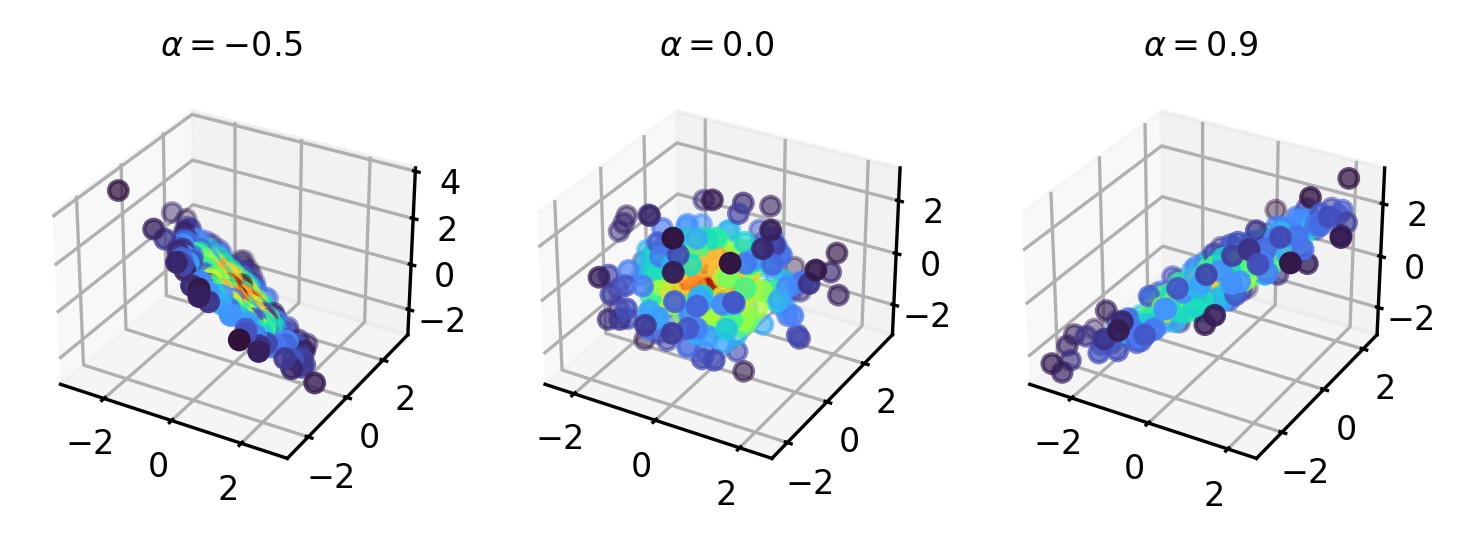
\includegraphics[width=15cm]{data_simulation/images/multivariate_normal/multivariate_normal.png}}
	\caption{Points drawn from a centered three-variate normal distribution with unit variance in the case of negative correlation (\emph{left}), zero correlation (\emph{center}) and positive correlation (\emph{right}). The points' color signify the probability density at that location.}
	\label{fig:data_simulation:multivariate_normal}
\end{figure}

For correlated noise, the problem at hand is similar: For multiple detectors, noise time-series $n_i$ should be simulated from a \emph{spectral matrix} $\underline{\underline{S_n}}$. This matrix contains each detector's noise PSD on its diagonal and the \emph{cross spectral densities} (CSDs) between detectors on the off-diagonal entries. For ET, that means three detectors, assuming the same PSD as in the uncorrelated case is each detector, $S_n^{ii} = S_n$ for $i=1,2,3$.
The CSDs are given by $S_n^{ij} = \alpha_{ij}\surd{S_n^{ii}S_n^{jj}} = \alpha_{ij} S_n$ with some correlation coefficient $\alpha_{ij}$. For the sake of simplicity, the same correlation is assumed between all detectors. Then, the spectral matrix can be written as
\begin{equation}
	\underline{\underline{S_n}} = \begin{pmatrix}
		S_n^{11} & S_n^{12} & S_n^{13} \\
		S_n^{21} & S_n^{22} & S_n^{23} \\
		S_n^{31} & S_n^{32} & S_n^{33}
	\end{pmatrix} 
	= \begin{pmatrix}
		1 & \alpha & \alpha \\
		\alpha & 1 & \alpha \\
		\alpha & \alpha & 1
	\end{pmatrix}\,S_n,
\end{equation}
with $\alpha$ bounded to a range between $-0.5$ and $1$. % One-liner, why that is the case
For a proof, see the \cite{PhysRevD.110.104060}.

An ansatz similar to Eq.~\ref{eq:data_simulation:uncorrelated_noise_dft_ansatz} is made for each detector's noise Fourier transform, 
\begin{equation}
	\tilde{n}_i(f) = a_i (x_i + iy_i).
\end{equation}
But now, the random variates $x_i$ and $y_i$ for each detector are not drawn independently of each other. Rather, vectors $\vec{x} = \begin{pmatrix} x_1 & x_2 & x_3 \end{pmatrix}^\intercal$ and $\vec{y} = \begin{pmatrix} y_1 & y_2 & y_3 \end{pmatrix}^\intercal$ are drawn from a \emph{multivariate} (in this case three-variate) normal distribution again with zero mean and unit variance, \emph{i.e.}, with a \emph{covariance matrix} that is given by
\begin{equation}
	\Sigma = \begin{pmatrix}
		1 & \alpha & \alpha \\
		\alpha & 1 & \alpha \\
		\alpha & \alpha & 1
	\end{pmatrix}.
\end{equation}
% \emph{i.e.}\ $x, y \sim \mathcal{N}(\mu=0, \Sigma)$
For a visualization of this distribution, see Fig.~\ref{fig:data_simulation:multivariate_normal}.
% Describe what we are seeing in this plot
Again, for each detector Eq.~\ref{eq:data_simulation:psd_relationship} should hold. Since $\langle x_i^2\rangle = 1$, the same formula for $a_i$ is recovered as in Eq.~\ref{eq:data_simulation:prefactor}. Then, the inverse Fourier transform yields the desired time-series.

In practice, a small positive correlation of $\alpha=0.1$ is assumed in the regime where seismic and Newtonian noise is dominant, which is below frequencies of \SI{10}{\hertz}. For higher frequencies $\alpha=0$, in which case the covariance matrix collapses to an identity matrix and the probability distribution effectively behaves as three independent normal distributions. A lower frequency cutoff of \SI{4}{\hertz} is applied, which means that the PSD is set to zero below that frequency. Furthermore, a sampling rate of \SI{2048}{\hertz} is chosen resulting in an upper resolution limit given by the Nyquist frequency, in this case \SI{1024}{\hertz}.  This is a reasonable resolution range, when considering BBH signals only. The inclusion of BNS signals in the simulation as well would necessitate a higher sampling rate. 
% The reasoning behind these frequency cuts has to do with the sort of signals that are simulated, which is the topic of the next chapter.
% TODO: plot noise with alpha=1 as sanity check, also plot realistic as is used in the simulations

\section{Gravitational Wave Signals}

It is important for the simulated dataset to cover all possible signal waveforms evenly such that when training neural networks no biases are learned. The shape of these waveforms will depend on a number of parameters, which are referred to as extrinsic and intrinsic. The former describe the signal source's location with respect to the detector reference frame and the latter are the intrinsic properties of the binary system, such as their masses.

\subsection*{Parameters}

\begin{figure}
	\centering
	\begin{minipage}{\textwidth}
		\centering
		\makebox[\textwidth]{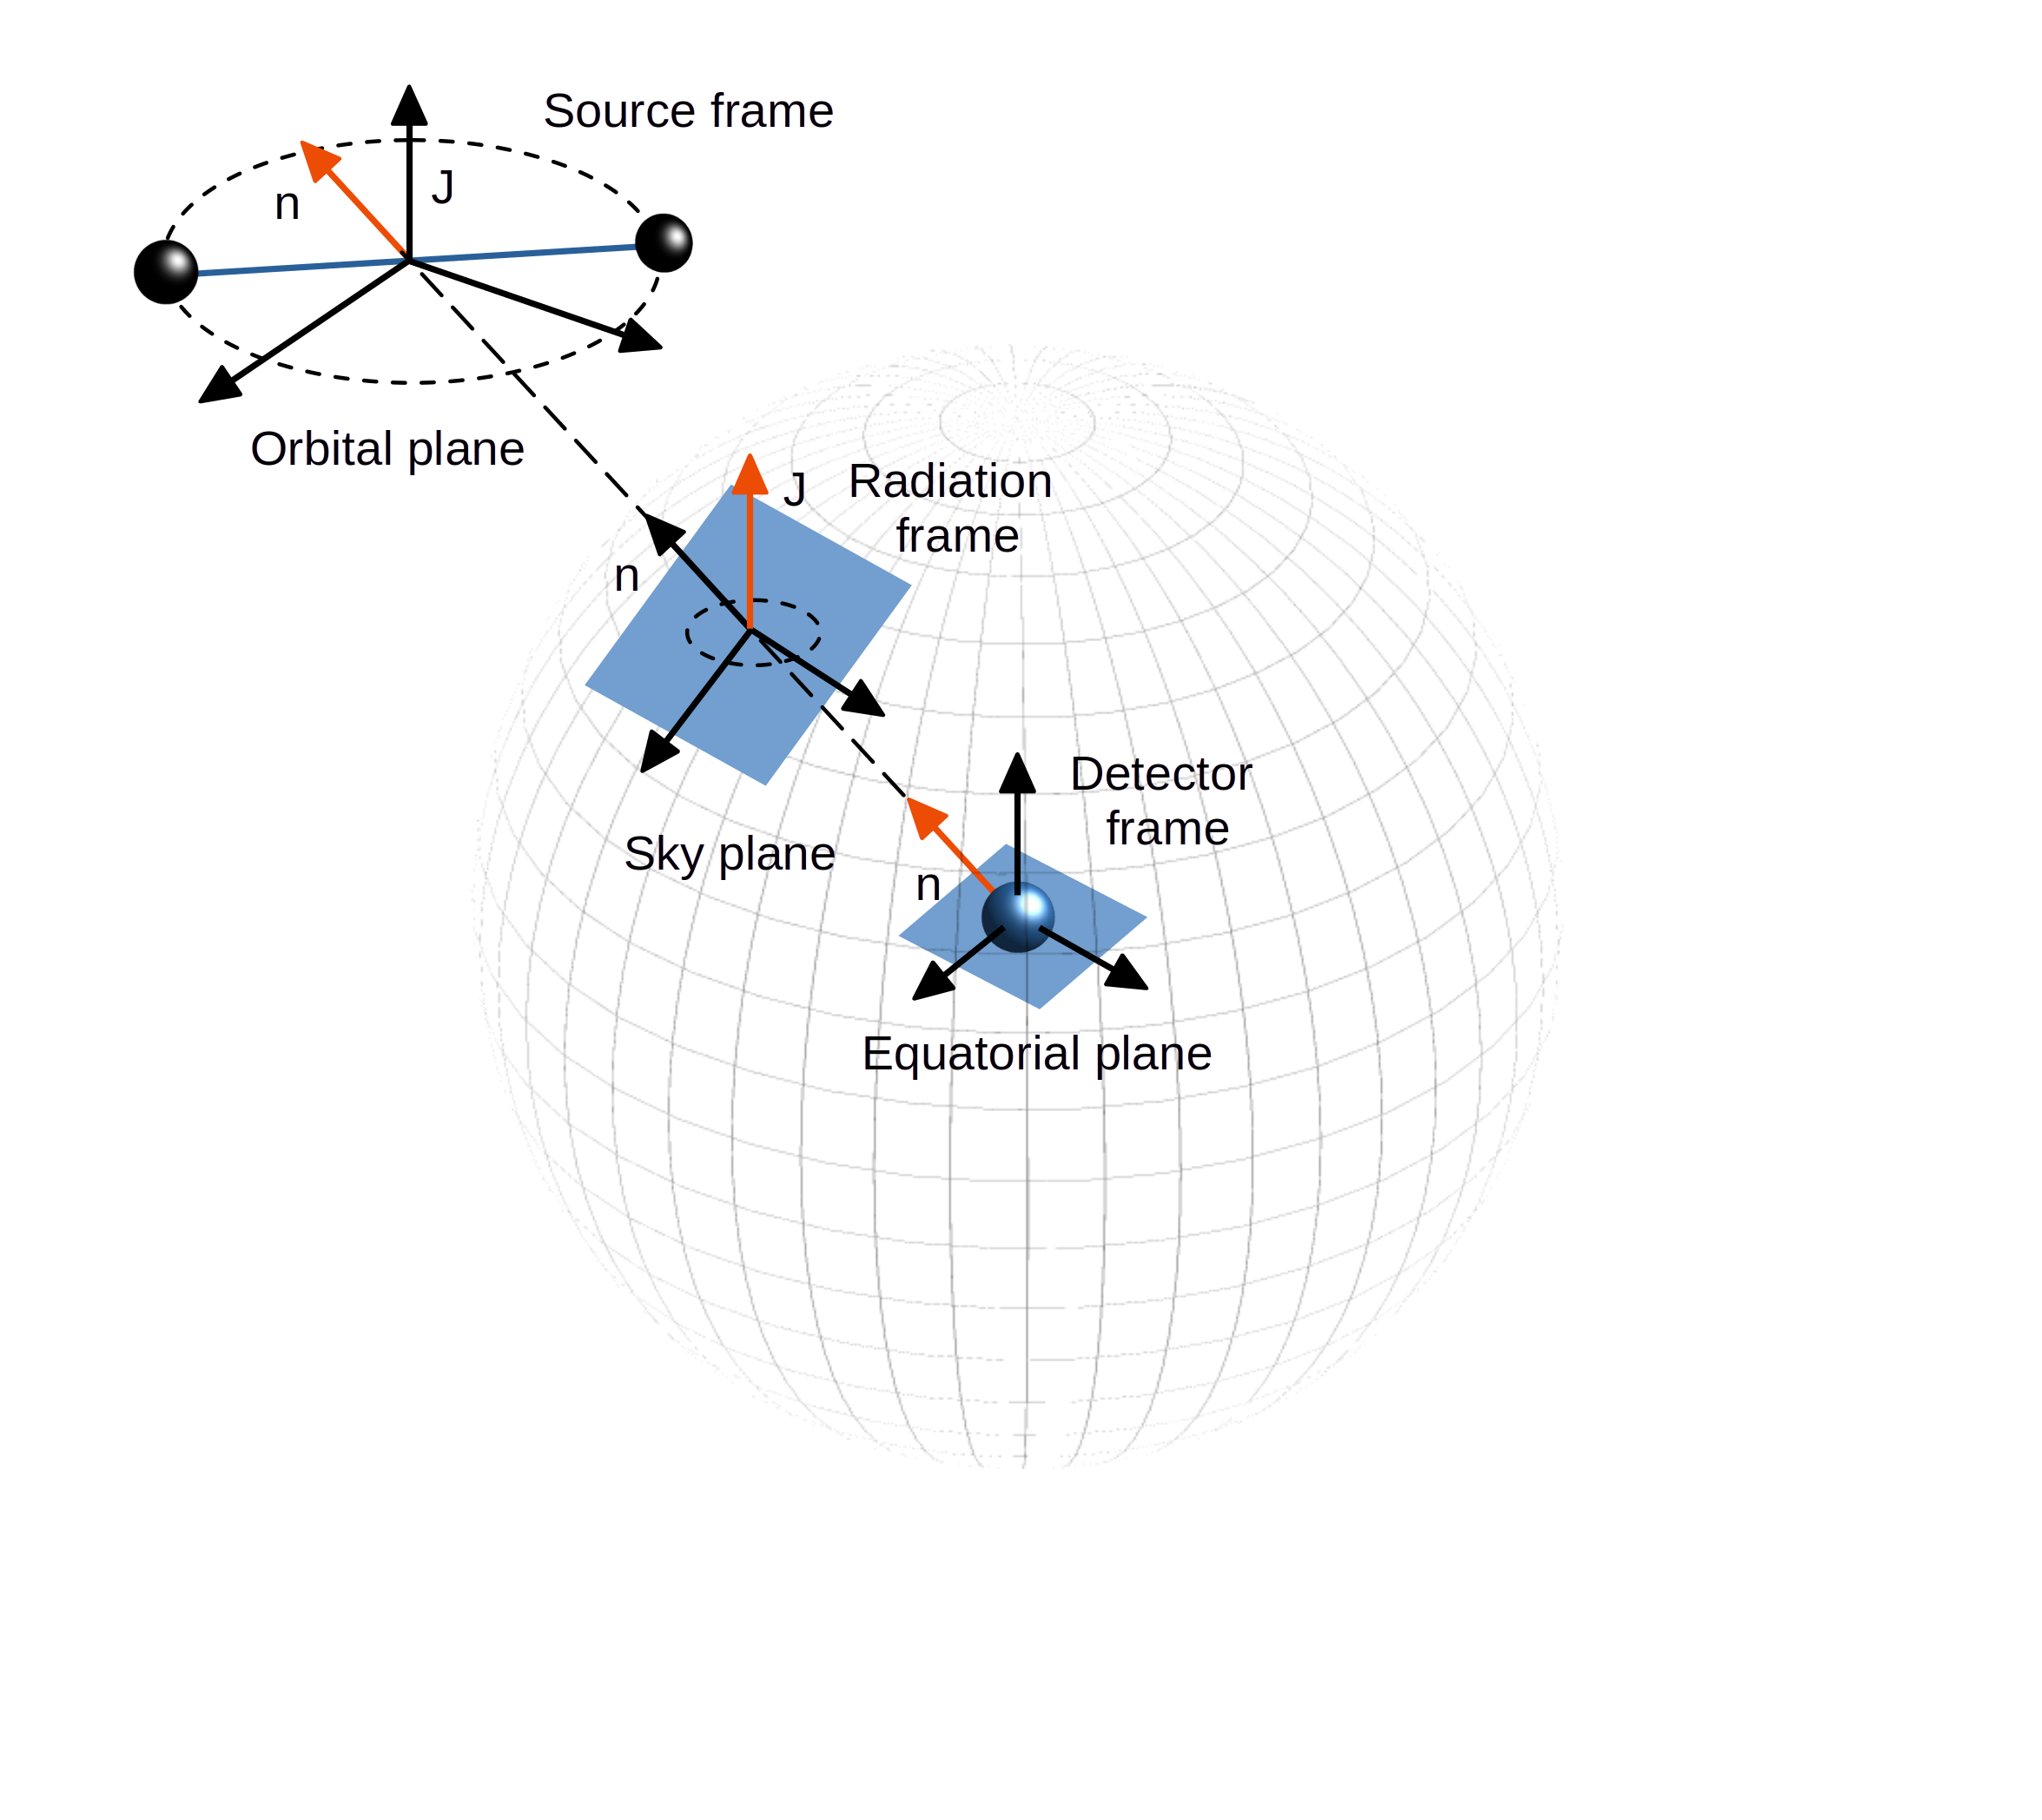
\includegraphics[width=10cm, trim=0 30cm 30cm 0, clip]{data_simulation/images/frames/frames_crop.png}}
		\caption{The three simulation frames. $\vec{n}$ is the line-of-sight vector that points towards the source. $\vec{J}$ denotes the binary's angular momentum vector.}
		\label{fig:data_simulation:frames}
	\end{minipage}
	\begin{minipage}{\textwidth}
		\centering
		\makebox[\textwidth]{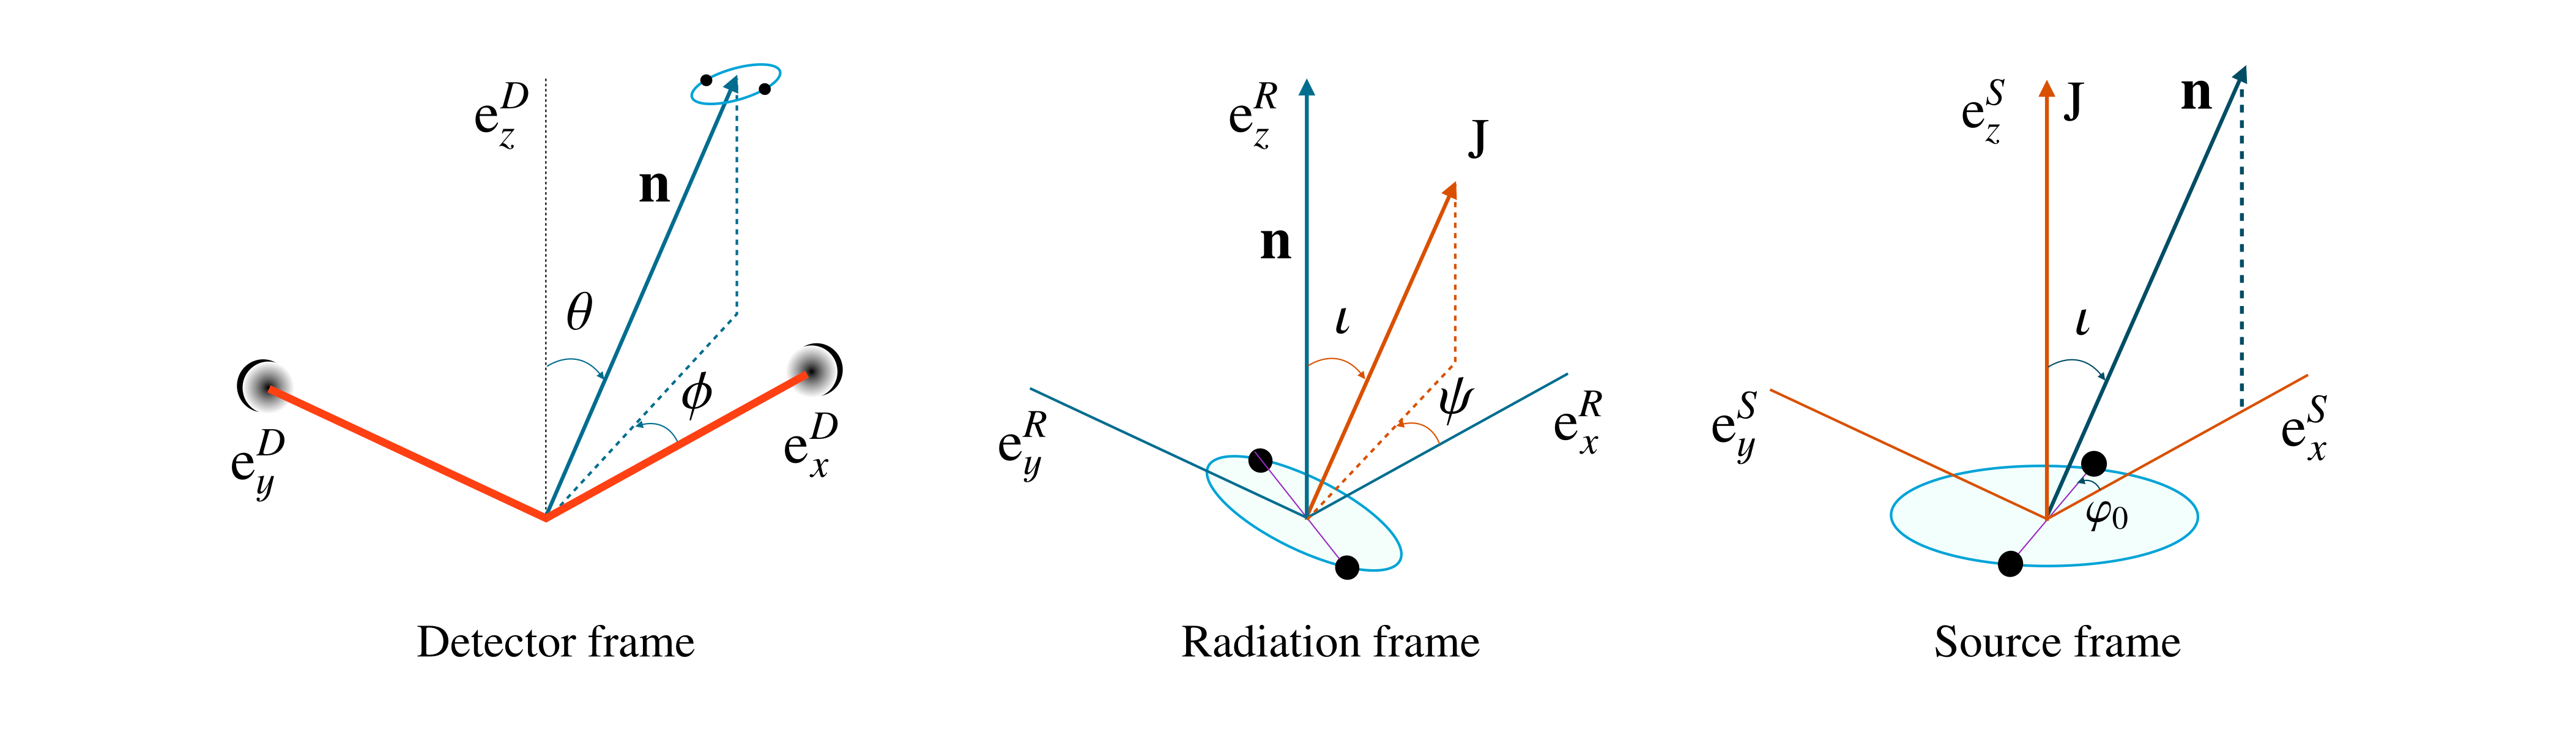
\includegraphics[width=18cm]{data_simulation/images/parameters/Detector-frame-The-two-orthogonal-arms-of-the-interferometer-form-the-x-and-y-axes-in_high_res.png}}
		\caption{The extrinsic parameters as defined within the three simulation frame. Here, the detector frame is defined by the interferometer geometry, which is not the convention this thesis follows. Taken from \cite{PhysRevD.90.124004}.}
		\label{fig:data_simulation:parameters}
	\end{minipage}
\end{figure}

The extrinsic parameters are defined through three simulation frames, the detector frame, the radiation frame and the source frame. In this thesis, the detector frame is the Equatorial coordinate system. This frame has a z-axis pointing towards the Earth's north pole, and an x-axis that points towards the March equinox. The y-axis is determined by the right circular convention.
The radiation frame can be thought of as the sky projection of the detector frame. Its z-axis is the line-of-sight vector towards the GW source. The x-axis is the projection of the detector frame's x-axis onto the sky plane, and the y-axis is again known by convention. The source frame has a z-axis pointing along the binary's orbital momentum vector. It x--y plane is the orbital plane, where the x-axis the projection of the line-of-sight vector.
See a schematic of the simulation frames in Fig.~\ref{fig:data_simulation:frames}.

There are a total of seven extrinsic parameters. The polar coordinates of the line-of-sight vector, \emph{i.e.}\ the inverse GW propagation direction, are the declination $\theta$ and the right ascension $\phi$. These two angles are defined with respect to the detector frame. 
The orientation of the binary with respect to the radiation frame yields two more parameters, the inclination $\iota$ and the polarization $\psi$. These are the polar angles of the source frame's z-axis, \emph{i.e.}\ the binary plane's normal vector, defined within the radiation frame. 
The other three parameters are the distance between detector and source $d$, as well as the coalescence time $t_\text{coa}$ and corresponding coalescence phase $\phi_\text{coa}$. The latter is the polar angle of primary mass in the source frame. The definition of the angle parameters are shown in Fig.~\ref{fig:data_simulation:parameters}.

The binary system has six intrinsic parameters. 
These include the two masses, the larger of which is called the primary mass $m_1$ by convention. (The other one is denoted $m_2$.) These masses can have non-zeros spins, which are described by the two vectors $\vec{S}_1$ and $\vec{S}_2$. The spins are defined within the source frame. In practice it is useful to define the dimensionless spin as $\vec{\chi}_i = \vec{S}_i / m_i^2$ with $|\vec{\chi}_i| < 1$ (in natural units that is).

\subsection*{Waveform Simulation}

For the simulation of gravitational wave signals from the inspiral, merger and ringdown of black hole binaries, the phenomenological model \emph{IMRPhenomD} \cite{PhysRevD.93.044007} is used as implemented by \emph{lalsimulation}. This is part of the LIGO Algorithm Library \cite{lalsuite}, which in turn is accessed via PyCBC.

These simulations take all the intrinsic parameters as inputs, which are the masses and spins.
The black hole mass distribution is modeled after CBC detections made by the second-generation network so far (see Fig.~\ref{fig:einstein_telescope:population}). Both black hole masses sampled uniformly in $[\SI{10}{\solarmass}, \SI{80}{\solarmass}]$, where the larger is the primary mass $m_1$ and the other $m_2$. 
This roughly corresponds to coalescence frequencies in a range of $[\SI{30}{\hertz}, \SI{220}{\hertz}]$ (see Eq.~\ref{eq:theory_of_gravitational_waves:max_freq_approx}), making the chosen sampling rate of \SI{2048}{\hertz} appropriate.
In the scope of this work, only aligned spin BBHs are considered, which means $\chi^i_x = \chi^i_y = 0$ and $\chi^i_z \geq 0$. The z-component of the spin is sampled uniformly in $[0, 0.998]$ with an upper limit that equals the Thorne limit. 

\begin{figure}
	\centering
	\begin{minipage}{\textwidth}
		\centering
		\makebox[\textwidth]{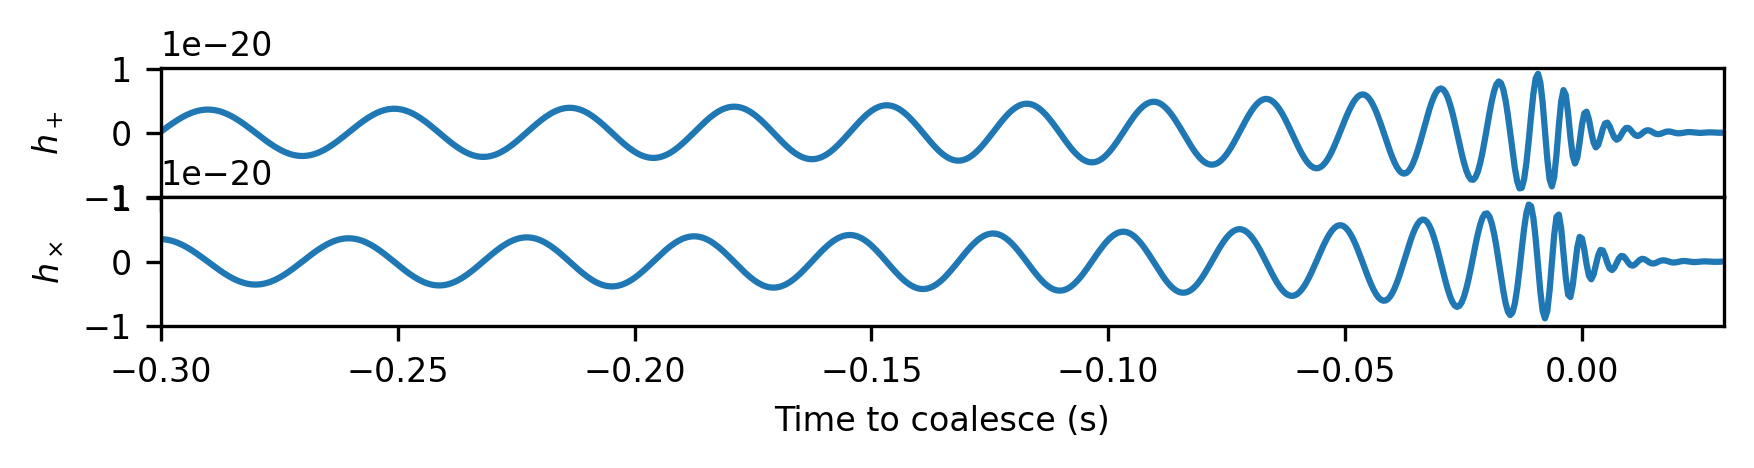
\includegraphics[width=15cm]{data_simulation/images/waveforms/waveform.png}}
		\caption{The plus and cross polarization strain of a GW signal emitted by a black-hole binary with masses $m_1 = \SI{50}{\solarmass}$, $m_2 = \SI{40}{\solarmass}$ and spins $\chi^1_z = 0.73$, $\chi^2_z = 0.43$ at a distance of \SI{100}{\mega\parsec}.}
		\label{fig:data_simulation:waveform}
	\end{minipage}
	\begin{minipage}{\textwidth}
		\centering
		\makebox[\textwidth]{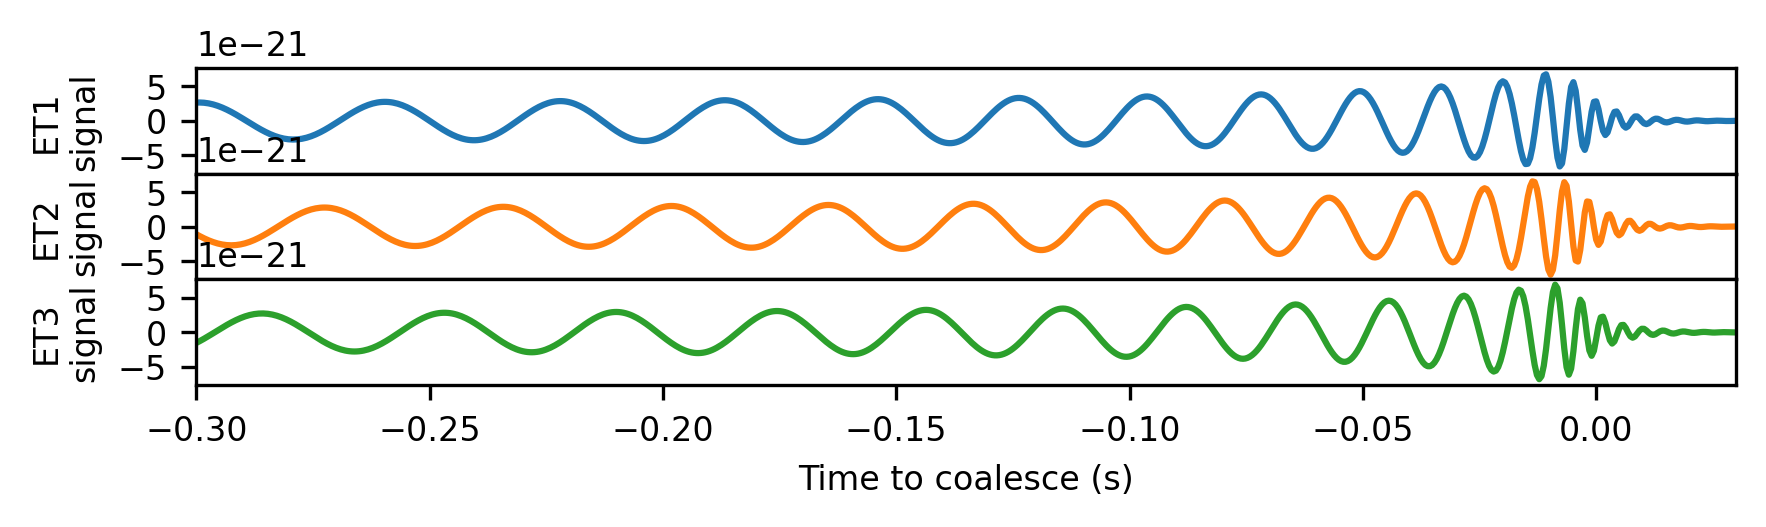
\includegraphics[width=15cm]{data_simulation/images/waveforms/projection.png}}
		\caption{The same GW signal from Fig.~\ref{fig:data_simulation:waveform} projected onto the three ET detectors as having a sky location $\phi = \SI{263}{\degree}$, $\theta = \SI{56}{\degree}$ and a polarization that is $\psi = \SI{78}{\degree}$.}
		\label{fig:data_simulation:projection}
	\end{minipage}
\end{figure}

The radiation pattern of the binary also depends on the binary's inclination and the coalescence phase. The inclination $\iota$ is sampled from a sine distribution with a probability density function proportional to $\sin{x}$ for $x$ in $[0, \pi]$.
The coalescence phase $\varphi_\text{coa}$ is sampled uniformly in $[0, 2\pi)$. 
Another simulation input parameter is the source distance. Since only the total strain amplitude depends on that distance and since there will be a rescaling step later anyway, the exact value is arbitrarily set to \SI{100}{\mega\parsec}. 
The simulation employs a lower frequency cutoff, which is the starting frequency of the waveform, which is set to \SI{4}{\hertz}. 
A waveform with all these parameters sampled accordingly can be seen plotted in Fig.~\ref{fig:data_simulation:waveform}.

\subsection*{Antenna Projection}

% for some reasons lalsimulation implements ET as being at 43.6314°N 10.5045°E, which is the site of VIRGO, see Einstein Telescope pre-site selection detector locations technical document LIGO DCC: T1400308

The simulated waveform are projected onto the ET interferometers to yield the GW strain according to Eq.~\ref{eq:einstein_telescope:antenna_functions}.
A PyCBC routine is relied upon to handle these antenna projections. The package implements ET according to \cite{T1400308} as three detectors in a triangular configuration with \SI{10}{\kilo\meter}-long arms. The detector is located at \SI{43.6314}{\degreeLat} \SI{10.5045}{\degreeLong}, which is the site of Virgo. 

PyCBC takes as input the detector GPS location, the GW signal sky position (in the equatorial frame) and the polarization.
In the simulation, the sky location is sampled uniformly. This means, the declination $\theta$ is sampled from a sine distribution and the right ascension $\phi$ uniformly in $[0, 2\pi)$. The GW polarization $\psi$ is sampled in $[0, 2\pi)$.
The routine further depends on the GW arrival time, for which PyCBC calculates the revolution of the Earth and updates the detector GPS location accordingly.
Since the GW sky position is sampled uniformly anyway, the arrival time is arbitrarily chosen to be zero. 
A GW signal that is projected as such is plotted in Fig.~\ref{fig:data_simulation:projection}.

\subsection*{Waveform Tapering}

The waveform simulation starts at the lower frequency cutoff, which is set to \SI{4}{\hertz}. This results in an \enquote{abrupt} jump in strain amplitude once the signal sets in which is an unphysical signature a neural network might pick up on easily. To mitigate this a tapering of the waveform is implemented by multiplying with a one-sided Tukey window:
\begin{equation}
	w(x) = \begin{cases}
		\frac{1}{2}(1-\cos{\frac{2\pi}{\alpha}\,x}) & \text{if } 0\leq x <\frac{\alpha}{2}\\
		1 & \text{if } \frac{\alpha}{2}\leq x<1.
	\end{cases}
\end{equation}
Here, $x$ is in units of total waveform length, \emph{i.e.}, $x=0$ corresponds to the beginning and $x=1$ to the end of the waveform. $\alpha = 1/4$ is chosen which means that the smoothing extends up to one eighth of the waveform. This trick is borrowed from \cite{PhysRevD.100.063015}.

\subsection*{SNR Rescaling}

In order to ease training for the neural networks, the dataset should include signals with a \enquote{loudness} that is evenly distributed. Preferably in a range, where detection is neither impossible nor trivial. To achieve this, the waveforms are rescaled by some factor $\beta$. 
A measure for the signal loudness is the optimal SNR (see Sec.~\ref{sec:matched_filtering}). This is denoted $\rho$ instead of $\rho_\text{opt}$ from now on. For multiple detectors the optimal SNR is,
\begin{equation}
	\rho^2 = \rho^2_1 + \rho^2_2 + \rho^2_3,
\end{equation}
with $\rho^2_i$ denoting the SNR of each of the three ET detectors. The individual detector SNR is given by Eq.~\ref{eq:matched_filtering:snr}, or in discrete form by,
\begin{equation}
	\rho^2_i = 4 \sum_j \Delta f \frac{|\tilde{h}_i(f_j)|^2}{S_n(f_j)}.
\end{equation}
Rescaling the signal amplitude by some positive factor $h_i(t)\rightarrow\beta h_i(t)$, means that the Fourier transform scales as, $\tilde{h}_i(f)\rightarrow\beta\tilde{h}_i(f)$. Thus, the individual detector SNRs scale as, $\rho_i\rightarrow\beta\rho_i$ and finally the total SNR as, $\rho\rightarrow\beta\rho$. That is to say, the signal waveform can just be rescaled by some positive prefactor to ensure a desired SNR. This prefactor is then given by $\beta = \rho / \rho'$, where $\rho$ is the desired SNR and $\rho'$ the SNR prior to rescaling. This desired SNR is sampled uniformly in $[5, 15]$. Signals with an SNR of $\sim5$ are more or less not detectable with matched filtering. For SNRs over $\sim10$, matched filtering reaches close to perfect detection ratios \cite{Nitz_2017}. GW150914 was observed with an total SNR of $24$ \cite{PhysRevLett.116.061102}.

In the case of correlated noise, this SNR formula does not hold anymore. Instead, as proposed in \cite{PhysRevD.110.104060}, the SNR is given by,
\begin{equation}
	\label{eq:data_simulation:correlated_snr}
	\rho^2 = 4 \Delta f \sum_k \sum_{i,j}
	\tilde{h}_i(f_k)^*(\underline{\underline{S_n}}^{-1})_{ij}(f_k)\tilde{h}_j(f_k),
\end{equation}
where $i,j$ sum over all detector combinations and $\underline{\underline{S_n}}^{-1}$ is the inverse spectral matrix,
\begin{equation}
	\underline{\underline{S_n}}^{-1} = \frac{1}{2\alpha^2 - \alpha - 1}
	\begin{pmatrix}
		-\alpha-1 & \alpha & \alpha \\
		\alpha & -\alpha-1 & \alpha \\
		\alpha & \alpha & -\alpha-1
	\end{pmatrix} \frac{1}{S_n}.
\end{equation}
Fortunately, since $\rho^2 $ is just a linear combination over all $\tilde{h}_i(f)^*\tilde{h}_j(f)$, rescaling with $\beta = \rho / \rho'$ is still valid. The difference is only that the pre-rescaling SNR $\rho'$ is calculated using the adapted SNR formula, \emph{i.e.}\ Eq.~\ref{eq:data_simulation:correlated_snr}.

\section{Samples and Datasets}

The datasets are built from multiple samples. Each sample resembles ET detector stream data of some length. To this end, partially correlated noise of that length is simulated and a number of GW signals are \emph{injected}, which simply means added. The waveform parameters are drawn randomly as described previously. For better clarity, the parameter distributions are restated in Tab.~\ref{tab:data_simulation:waveform_parameters}. The signals are injected with random coalescence times, covering the whole length of the detector stream. 

\begin{table}[]
	\centering
	\caption{Simulation waveform parameter distributions.}
	\label{tab:data_simulation:waveform_parameters}
	\begin{tabular}{l c l}
		\toprule
		\multicolumn{2}{c}{Waveform parameter} & Distribution \\
		\midrule
		Masses & $m_1$, $m_2$ 
		& $\text{Uniform}(\SI{10}{\solarmass}, \SI{80}{\solarmass})$ \\
		Non-aligned spins & $\chi_x$, $\chi_y$
		& $0$ \\
		Aligned spins & $\chi_z$
		& $\text{Uniform}(0, 0.998)$ \\
		Sky position & $\theta$, $\phi$
		& $\text{Sine}(0, \pi)$, $\text{Uniform}(0, 2\pi)$ \\
		Inclination and polarization & $\iota$, $\psi$
		& $\text{Sine}(0, \pi)$, $\text{Uniform}(0, 2\pi)$ \\
		Coalescence phase & $\varphi_\text{coa}$
		& $\text{Uniform}(0, 2\pi)$ \\
		Optimal SNR & $\rho$
		& $\text{Uniform}(5, 15)$ \\
		
		\bottomrule
	\end{tabular}
\end{table}
In this work, the task of detecting multiple long-duration signals will be split in two steps. First, the simplified problem of detecting one long-duration signal per sample is considered. This allows testing different architectures, while increasing the sample length. To fit a full BBH waveform, a final sample length of $\approx\SI{1}{\minute}$ is aimed for. Multiple datasets with increasing length are constructed. For better comparability, training datasets will always consist of \SI{1}{\mega\nothing} samples in this thesis. Since there is only up to one signal per sample, this task can be simplified to a \emph{binary-classification} problem. In this case, the network will predict one number per sample that signifies whether there is signal in the given detector stream or not. Samples with no injection will be labeled \emph{negative}, \emph{i.e.}\ $0$, and samples with an injected signal \emph{positive}, \emph{i.e.}\ $1$. To avoid learned biases, the dataset will be constructed evenly, that is, half of the samples will be positive and the other half negative.

\begin{figure}
	\centering
	\makebox[\textwidth]{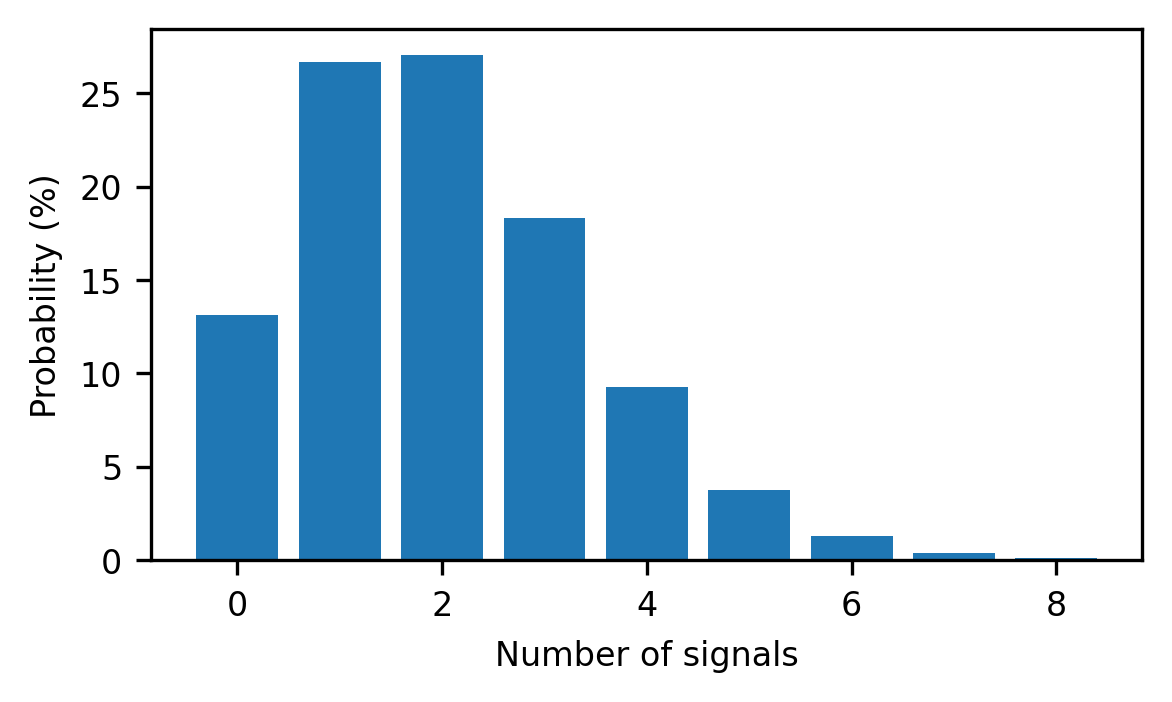
\includegraphics[width=10cm]{data_simulation/images/poisson/poisson}}
	\caption{Probability of $n$ number of signals in a \SI{64}{\second} sample of ET detector stream, assuming the higher event rate estimate of \SI{E+6}{\per\year}.}
	\label{fig:data_simulation:poisson}
\end{figure}

\begin{figure}
	\centering
	\makebox[\textwidth]{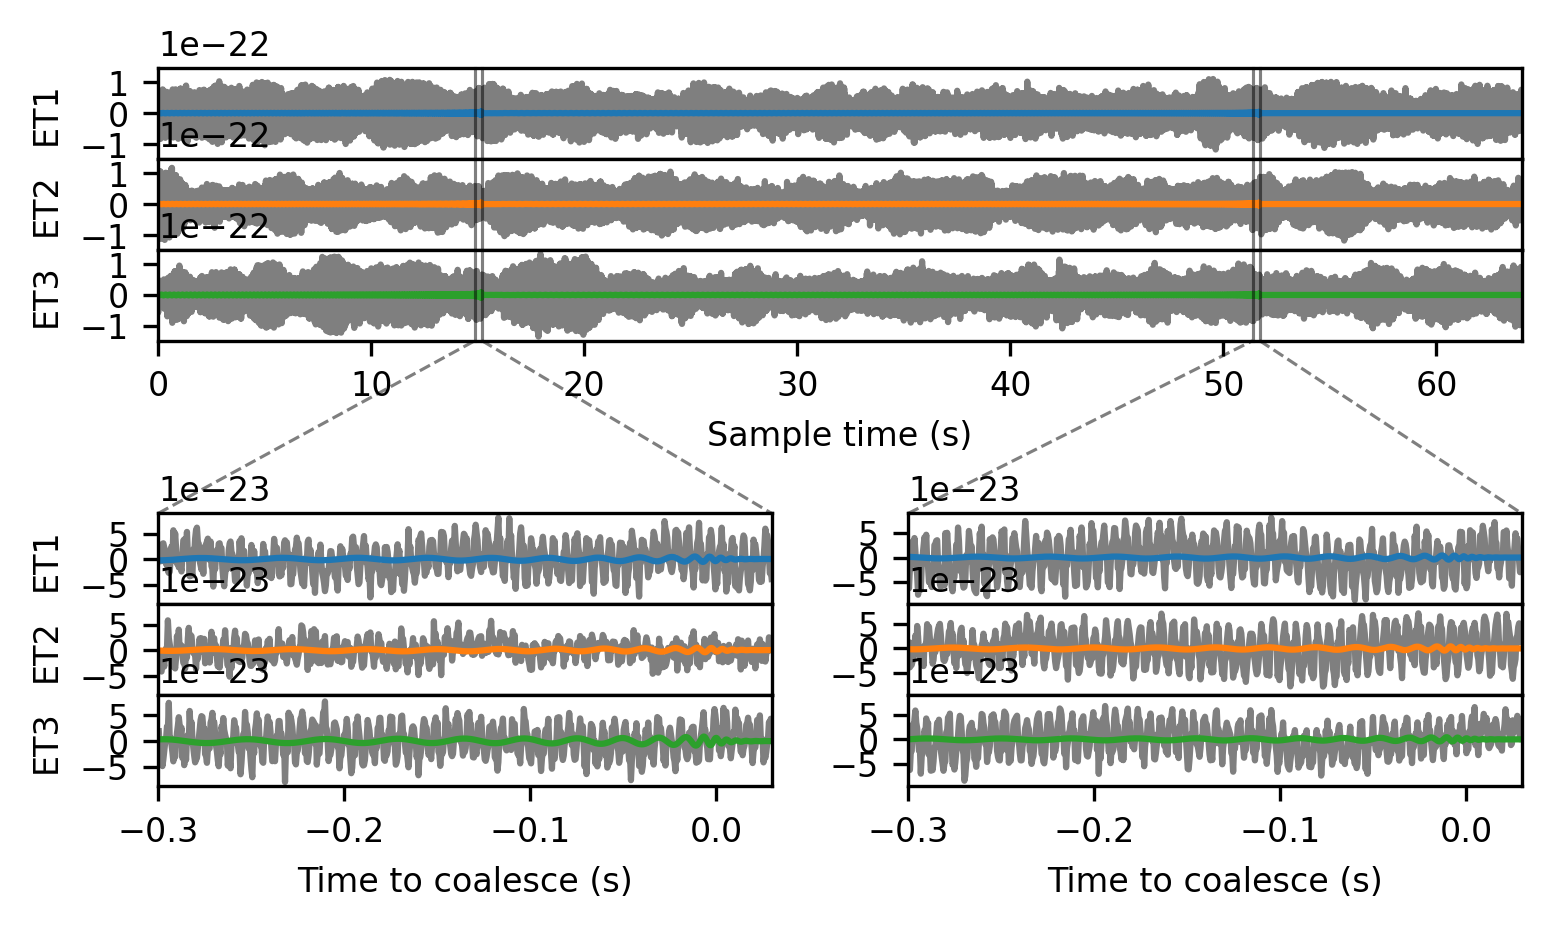
\includegraphics[width=15cm]{data_simulation/images/waveforms/injection.png}}
	\caption{Sample with two injected signals. The total strain is plotted in gray, and the signal contribution in color. The first signal has an SNR of $\approx6.4$, and the second one has $\approx9.1$.}
	\label{fig:data_simulation:injection}
\end{figure}

\begin{figure}
	\centering
	\makebox[\textwidth]{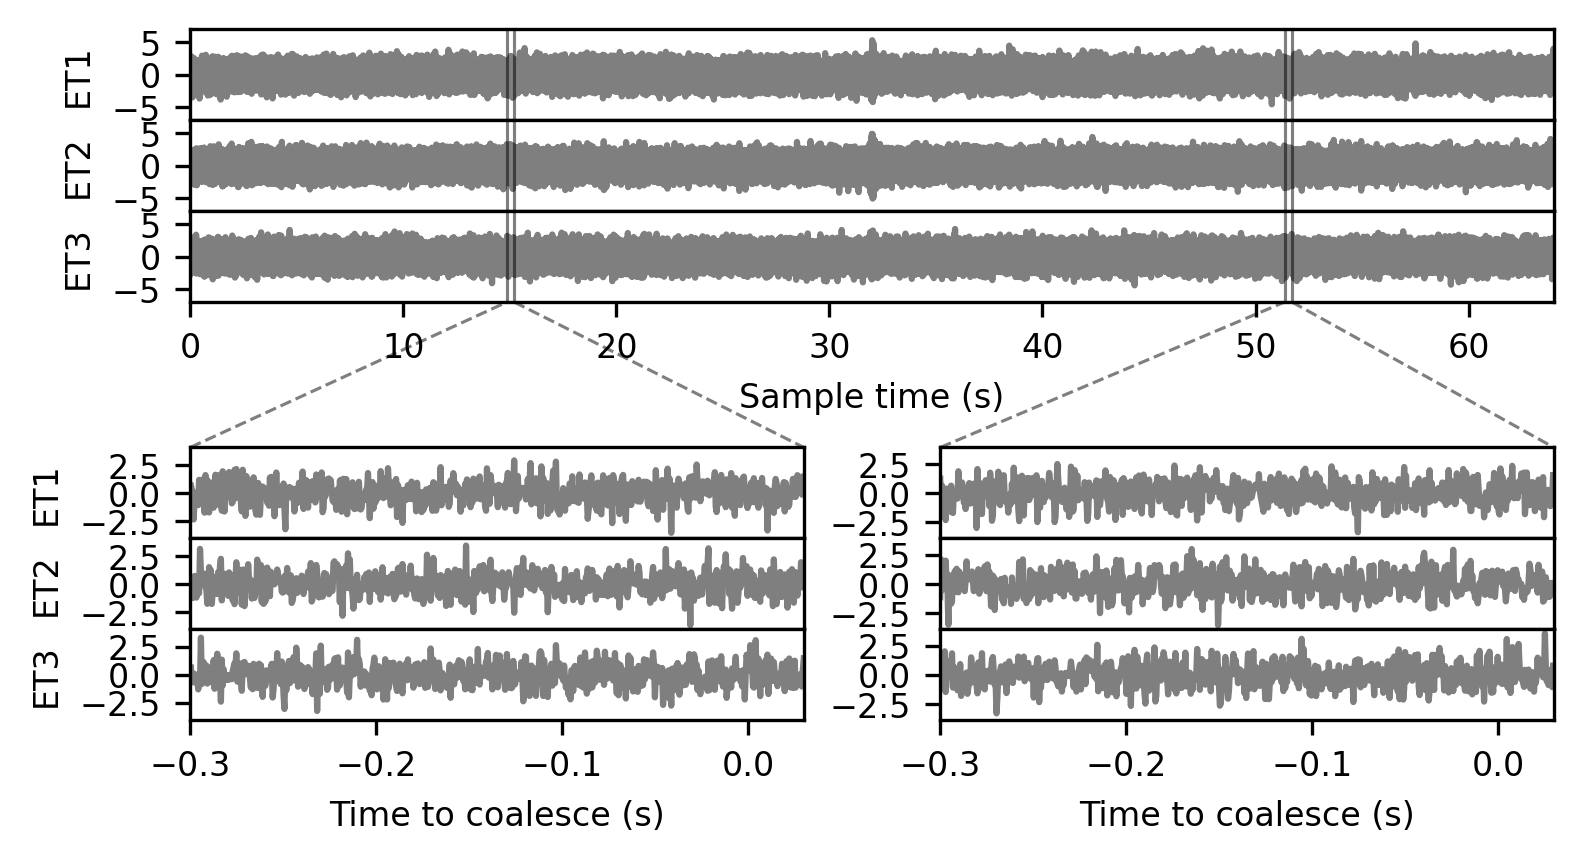
\includegraphics[width=15cm]{data_simulation/images/waveforms/sample.png}}
	\caption{The same sample as in Fig.~\ref{fig:data_simulation:injection} after whitening, band-passing and standardizing. This resembles the data that neural networks are trained on in this work.}
	\label{fig:data_simulation:sample}
\end{figure}

The second step deals with multiple such long-duration waveforms in a $\SI{64}{\second}$ sample. This case is treated similar to an \emph{object detection} task, where the network should predict multiple signals along with their coalescence time. To cover all cases evenly and ensure no biases are learned, the number signals per sample is sampled \emph{uniformly} in $[0, 6]$. The maximum of six signals is justified by the expected event rate in ET, which is up to $\lambda=\SI{E+6}{\per\year}$ signals. This is a Poissonian process, thus the probability of $n$ signals in one sample of length $T$ is,
\begin{equation}
 	P(n) = \frac{(\lambda\,T)^n}{n!}\,\e^{-\lambda\,T}.
\end{equation}
The distribution is visualized in Fig.~\ref{fig:data_simulation:poisson}. By choosing a maximum of six signals, most relevant cases are covered. See an example sample with two injected signals in Fig.~\ref{fig:data_simulation:injection}. Note that this neglects the simulation of signals with a merger time outside the sample window.

\section{Post-Processing}

Three post-processing steps are performed on the samples.
First, the data is \emph{whitened}. This step aims to turn the colored noise power spectrum into a white one, which is constant over the whole frequency regime. In theory, this can be achieved by down-weighting the strain's Fourier coefficients $\tilde{s}(f)$ by the noise amplitude spectral density, \emph{i.e.}\ the square root power spectral density $S_n$: 
\begin{equation}
	\tilde{s}'(f) = \frac{\tilde{s}(f)}{\sqrt{S_n(f)}}, 
\end{equation}
such that $S_n'(f) = 2\Delta f|\tilde{s}'(f)|^2 = 1$ in the absence of a signal.

In GW searches, the exact noise PSD is not known \emph{a priori} of course, and has to be estimated from the detector stream instead. To this end, an adaption from Welch's method is used, as implemented in PyCBC \cite{alex_nitz_2023_10013996}. This method splits the given detector strain into $N$ overlapping segments of some duration and with a stride that is half that duration. For each segment $i$, the PSD is computed as,
\begin{equation}
	S_n^i(f) = 2\Delta f|\tilde{s}^i(f)|^2.
\end{equation}
Then, an estimate of the noise PSD is the \emph{median} over all segments,
 \begin{equation}
 	S_n(f) = \frac{1}{\alpha}\,\text{median}(S_n^1(f), S_n^2(f), \dots), 
 \end{equation}
with a correction factor $\alpha = \sum_{i=1}^N (-1)^{i+1}/i$. The median instead of the mean is used to ensure that only the \emph{noise} PSD is estimated. The latter might be biased towards larger values in the presence of gravitational wave signals. 

In this thesis, the PSD is estimated for each detector and each sample separately.
This roughly mimics the procedure in real searches, where the PSD estimate is adjusted constantly.
Since the samples of some of the datasets are only a few seconds short, they are always simulated with some minimum length, over which the PSD is estimated, and later cut to the desired sample length. The minimum length is at least \SI{16}{\second} or twice the desired sample length. The extra is padded to both ends of the sample symmetrically, since the whitening procedure introduces corruption at both edges.

As another post-processing step the data is band-passed. The waveform fade-on can introduce frequency contributions below the frequency cut-off of \SI{4}{\hertz}, which might be a giveaway for the presence of a GW signal in the sample. Thus, the data is high-passed above \SI{4}{\hertz}. As this step also causes corruption at both ends of the sample, similar to whitening, the band-passing will be applied before cutting to the desired sample length.

The final processing step is standardizing the data. This is a common and often necessary data preparation step in a machine learning context, which ensures inputs with zero mean and unit variance. This is done for multiple samples at once, and for each detector  $i$ separately,
\begin{equation}
	s'_i(t) = \frac{s_i(t)-\mu_i}{\sigma_i},
\end{equation}
where $\mu_i$ and $\sigma_i$ denote the mean and standard deviation. These are computed over \SI{4096}{\nothing} samples each. See a post-processed sample in Fig.~\ref{fig:data_simulation:sample}. 
% The data includes whitening artefacts in the middle of each sample. These are caused by the harmonics of the noise PSD.



\chapter{Binary Classification}
\label{sec:long_duration}
% Why?
% 1) Long-duration signals -> long duration data needs to be processed (known to be hard for ML algorithms, see https://arxiv.org/pdf/2209.11146) \cite{Sch_fer_2023}
% 2) Increasing ML receptive field is necessary to capture multiple overlapping signals fully
% 3) In practice it was necessary to get the models to work on large input sizes first, before adding the challenge of detecting multiple signals in one sample

As previously mentioned, the task of detecting long-duration overlapping signals is split in two, focusing on the long-duration part first. In previous research, ML algorithms usually only process a short duration of data of a few seconds, which is sufficient for second-generation detectors, where signals are short \cite{George_2018, PhysRevD.100.063015}. In contrast, the increased signal duration in ET requires processing larger amounts of data at once. This study is concerned with increasing the processed duration up to \SI{1}{\minute}, comparable to the expected BBH signal length in ET.

% Multiple datasets with increasing sample length
% Try CNN (similar to previous research)
% State of the art: ResNet
% Try transformer architecture because it captures long range dependencies
% Image processing -> ViT

To this end, multiple datasets with increasing sample lengths are simulated. For the purposes of this study, every sample contains only one signal at most. The problem of detecting multiple signals per sample is dealt with in the next chapter. This study compares a CNN, the \emph{de facto} standard approach, and a transformer model when handling large inputs. 
Although \cite{Papalini_2025} motivates the use of transformers for overlapping signals primarily, the transformer's ability to capture long-range dependencies could outperform CNNs in this context. The code for all machine-learning models used in this thesis is available at \cite{git_models}.

\section{Problem Setup}

% Binary classification
% up to one signal per sample with random coalescence time

% Emphasize that this does not amount to a proper search, where we want to to identify the temporal location of potential signals in time series data of arbitrary length or in streaming data
A final sample length of \SI{64}{\second} is aimed for. With a sampling rate of \SI{2048}{\hertz}, and for three ET detectors, that means an input size of $3\times\SI{2048}{\hertz}\times\SI{64}{\second} = \SI{393}{\kilo\nothing}$. Compare this to standard image-classification models such as ResNets \cite{he2016residual}, which handle input sizes of $3\times224\times224=\SI{150}{\kilo\nothing}$.

This study considers datasets with sample lengths of \SI{2}{\second}, \SI{4}{\second}, \SI{8}{\second}, \SI{16}{\second}, \SI{32}{\second}, and \SI{64}{\second}. Each sample contains one signal at most, and these signals are injected uniformly over the whole sample length.
The task is treated as a binary classification problem: Noise samples are labeled $0$, and injection samples $1$. The datasets are even, \emph{i.e.}, half of the samples are positive and the other half negative. Training datasets have \SI{1}{\mega\nothing} samples each, and the test datasets \SI{131}{\kilo\nothing}. Both datasets are simulated in the same manner.

It should be emphasized that this does not amount to a proper GW signal search, since binary classification becomes insufficient for long data stretches, if the signal candidate is not accompanied by its time location in that data. Still, this simplification is sufficient for isolating the problem of processing large inputs.

% TP, FP, FN, TN -> threshold
Binary classification models usually return a continuous output $\hat{y}$ between $0$ and $1$, interpreted as a signal score. To obtain a binary prediction, this score is compared to a threshold. Model output values are labeled negative if below the threshold and positive else. 
Depending on the target or ground truth label of a sample, four cases can be identified:
\begin{center}
	\begin{tblr}{
			colspec={cc|cc},
			cells={c,m},
			cell{3}{3}={bg=gray!25},
			cell{4}{4}={bg=gray!25},
		}
		& & \SetCell[c=2]{c} Prediction $\hat{y}$ & \\
		& & 1 & 0 \\
		\hline
		\SetCell[r=2]{c} \rotatebox{90}{Target $y$}
		& 1
		& {True positive\\(TP)}
		& {False negative\\(FN)} \\
		& 0
		& {False positive\\(FP)}
		& {True negative\\(TN)}
	\end{tblr}
\end{center}
TPs and TNs correspond to a correct classification, while FPs and FNs are errors. Evaluated over all test samples, the table above forms a \emph{confusion matrix}.

Instead of consulting the confusion matrix for one particular threshold, it is often more insightful to plot the evolution of its entries for different thresholds. To this end, the true positive rate (TPR) and the false positive rate (FPR) are defined as
\begin{align}
	\mathrm{TPR} = \frac{\mathrm{TP}}{\mathrm{TP} + \mathrm{FN}}, \quad
	\mathrm{FPR} = \frac{\mathrm{FP}}{\mathrm{FP} + \mathrm{TN}}.
\end{align}
That is, the fraction of target positive samples that are correctly identified as such, and the fraction of target negatives that are incorrectly labeled positive. Plotting the set of $(\text{FPR}(z), \text{TPR}(z))$ for all thresholds $z\in[0,1]$ yields the \emph{receiver operating characteristic} (ROC). This curve shows a model's performance independent of the chosen threshold.

There are multiple ways to compare the performance of different models. For instance, the threshold could be chosen to ensure the same FPR for all models, and the corresponding TPR could be compared. (This is the way models will be compared in the next chapter, when implementing something closer to an actual search, in which case the algorithm's false alarm rate should be low to ensure confident detections.) In this study, models are simply compared by their AUROC, the area under the ROC,
\begin{align}
	\mathrm{AUROC} = \int_0^1 \mathrm{TPR}\,\mathrm{d}\mathrm{FPR}.
\end{align}
This metric returns \SI{100}{\percent} if the classifier is perfect, while a random classifier yields \SI{50}{\percent} AUROC.

\section{CNN and Transformer Models}

% CNN modeled after Resnet18 (fig)
% less parameters, more downsampling
% skip connections (see ResNet paper)
% check receptrive field
% global average pool + dense network
% 700k parameters
% number of parameters does not increase with input size 

This work employs a CNN that is modeled after the \emph{ResNet} architecture \cite{he2016residual}. ResNets improve the traditional CNN recipe by the first introduction of residual connections. These have later also been adapted in transformers (see Ch.~\ref{sec:machine_learning:transformers}). Such connections ease the training of deep CNNs by allowing the redundant layers to act as identity maps. 

Each convolutional block employs batch normalization~\cite{pmlr-v37-ioffe15} and uses the standard ReLU activation,
\begin{equation}
	\text{ConvBlock}(x) = \text{ReLU}(\text{BatchNorm}(\text{ConvLayer}(x))).
\end{equation}
There are residual connections every two blocks,
\begin{equation}
	\text{ResBlock}(x) = \text{ReLU}(\text{skip}(x) + \text{ConvBlock}(\text{ConvBlock}(x))).
\end{equation}
If the dimensions match, \emph{i.e.}, the convolutional blocks have stride one and the number of channels does not increase, $\text{skip}(x) = x$, else, it is obtained through a convolutional operation with kernel size one.

\begin{figure}
	\centering
	\makebox[\textwidth]{
		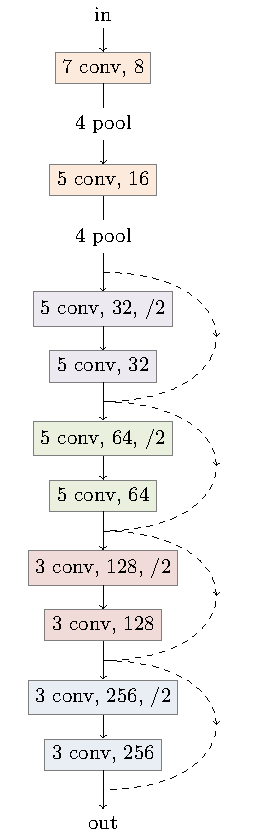
\includegraphics[width=113.6199pt]{machine_learning/images/resnet/custom}
		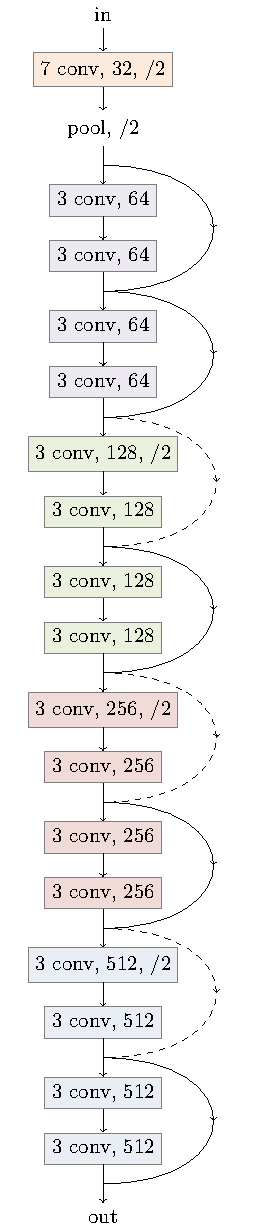
\includegraphics[width=116.11992pt]{machine_learning/images/resnet/resnet18}
		% 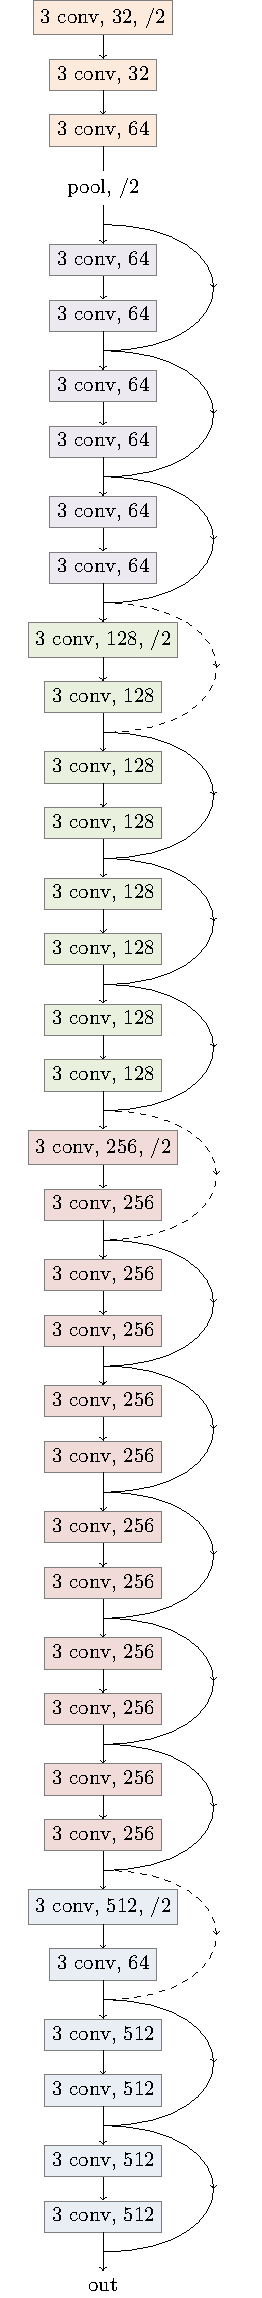
\includegraphics[width=116.11992pt]{machine_learning/images/resnet/resnet34}
	}
	\caption{The custom ResNet architecture that is employed in this work (\emph{left}) and ResNet18~\cite{he2016residual} (\emph{right}). One convolutional block is denoted \enquote{kernel size} conv, \enquote{out channels}, /\enquote{stride}. Skip connections are drawn as arrows. These are dashed if the dimensions do not match.}
	\label{fig:binary:resnet}
\end{figure}

The employed CNN is modeled after ResNet18, the smallest ResNet model with $18$ layers, which is adapted to fit this task's needs (see Fig.~\ref{fig:binary:resnet}). 
\begin{itemize}
\item The number of layers is reduced from $18$ to $12$, decreasing the total model size. The final network has \SI{700}{\kilo\nothing} trainable parameters. 
\item  More aggressive downsampling is implemented to handle the desired long inputs. The model downsamples its input by a factor $256$. For an input of size $3\times\SI{131}{\kilo\nothing}$ (the three detectors are treated as input channels), the model produces an output of shape $256\times512$.
\item  Kernel sizes are increased to enlarge the model's receptive field. This gives a total receptive field of $1766$ or roughly \SI{1}{\second}, which is more than enough to resolve the data's lowest frequencies of \SI{4}{\hertz}.
\end{itemize}
Following the ResNet architecture, \emph{global average pool} is applied over the time dimension of the $256$ feature maps. The output is fed to the classification head, a dense network, 
%\begin{equation}
%	z = \text{Linear}_{1024\rightarrow1}(\text{ReLU}(\text{Linear}_{256\rightarrow1024}(\text{Dropout}(x)))),
%\end{equation}
\begin{align}
	h &= \mathrm{Dropout}(\mathrm{ReLU}(\mathrm{Linear}_{256\rightarrow1024}(x))),\\
	z &= \mathrm{Dropout}(\mathrm{Linear}_{1024\rightarrow1}(h)),
\end{align}
producing single \emph{logit} as output. The dropout probability is \SI{10}{\percent}. A class score obtained through a sigmoid activation,
\begin{equation}
	\hat{y} = \text{Sigmoid}(z) = \frac{1}{1+\e^{-z}},
\end{equation}
which is bounded between $0$ and $1$. 
Note that the model's number of parameters is independent of the input size. This is obviously the case for the kernel parameters, but also for the classification head, since the time information is lost after global average pooling.

% CNN + Transformer hybrid (CNN stays the same)
% explain tokenization
% each downsampled timestep serves as one token
% projected onto model dimension with Conv1d

% Classification token (ViT)
% learned positional encodings

% number of heads and layers
% vram increases quadratically with input size
% 1.7m parameters, no increase with input size

\begin{figure}
	\centering
	\makebox[\textwidth]{
		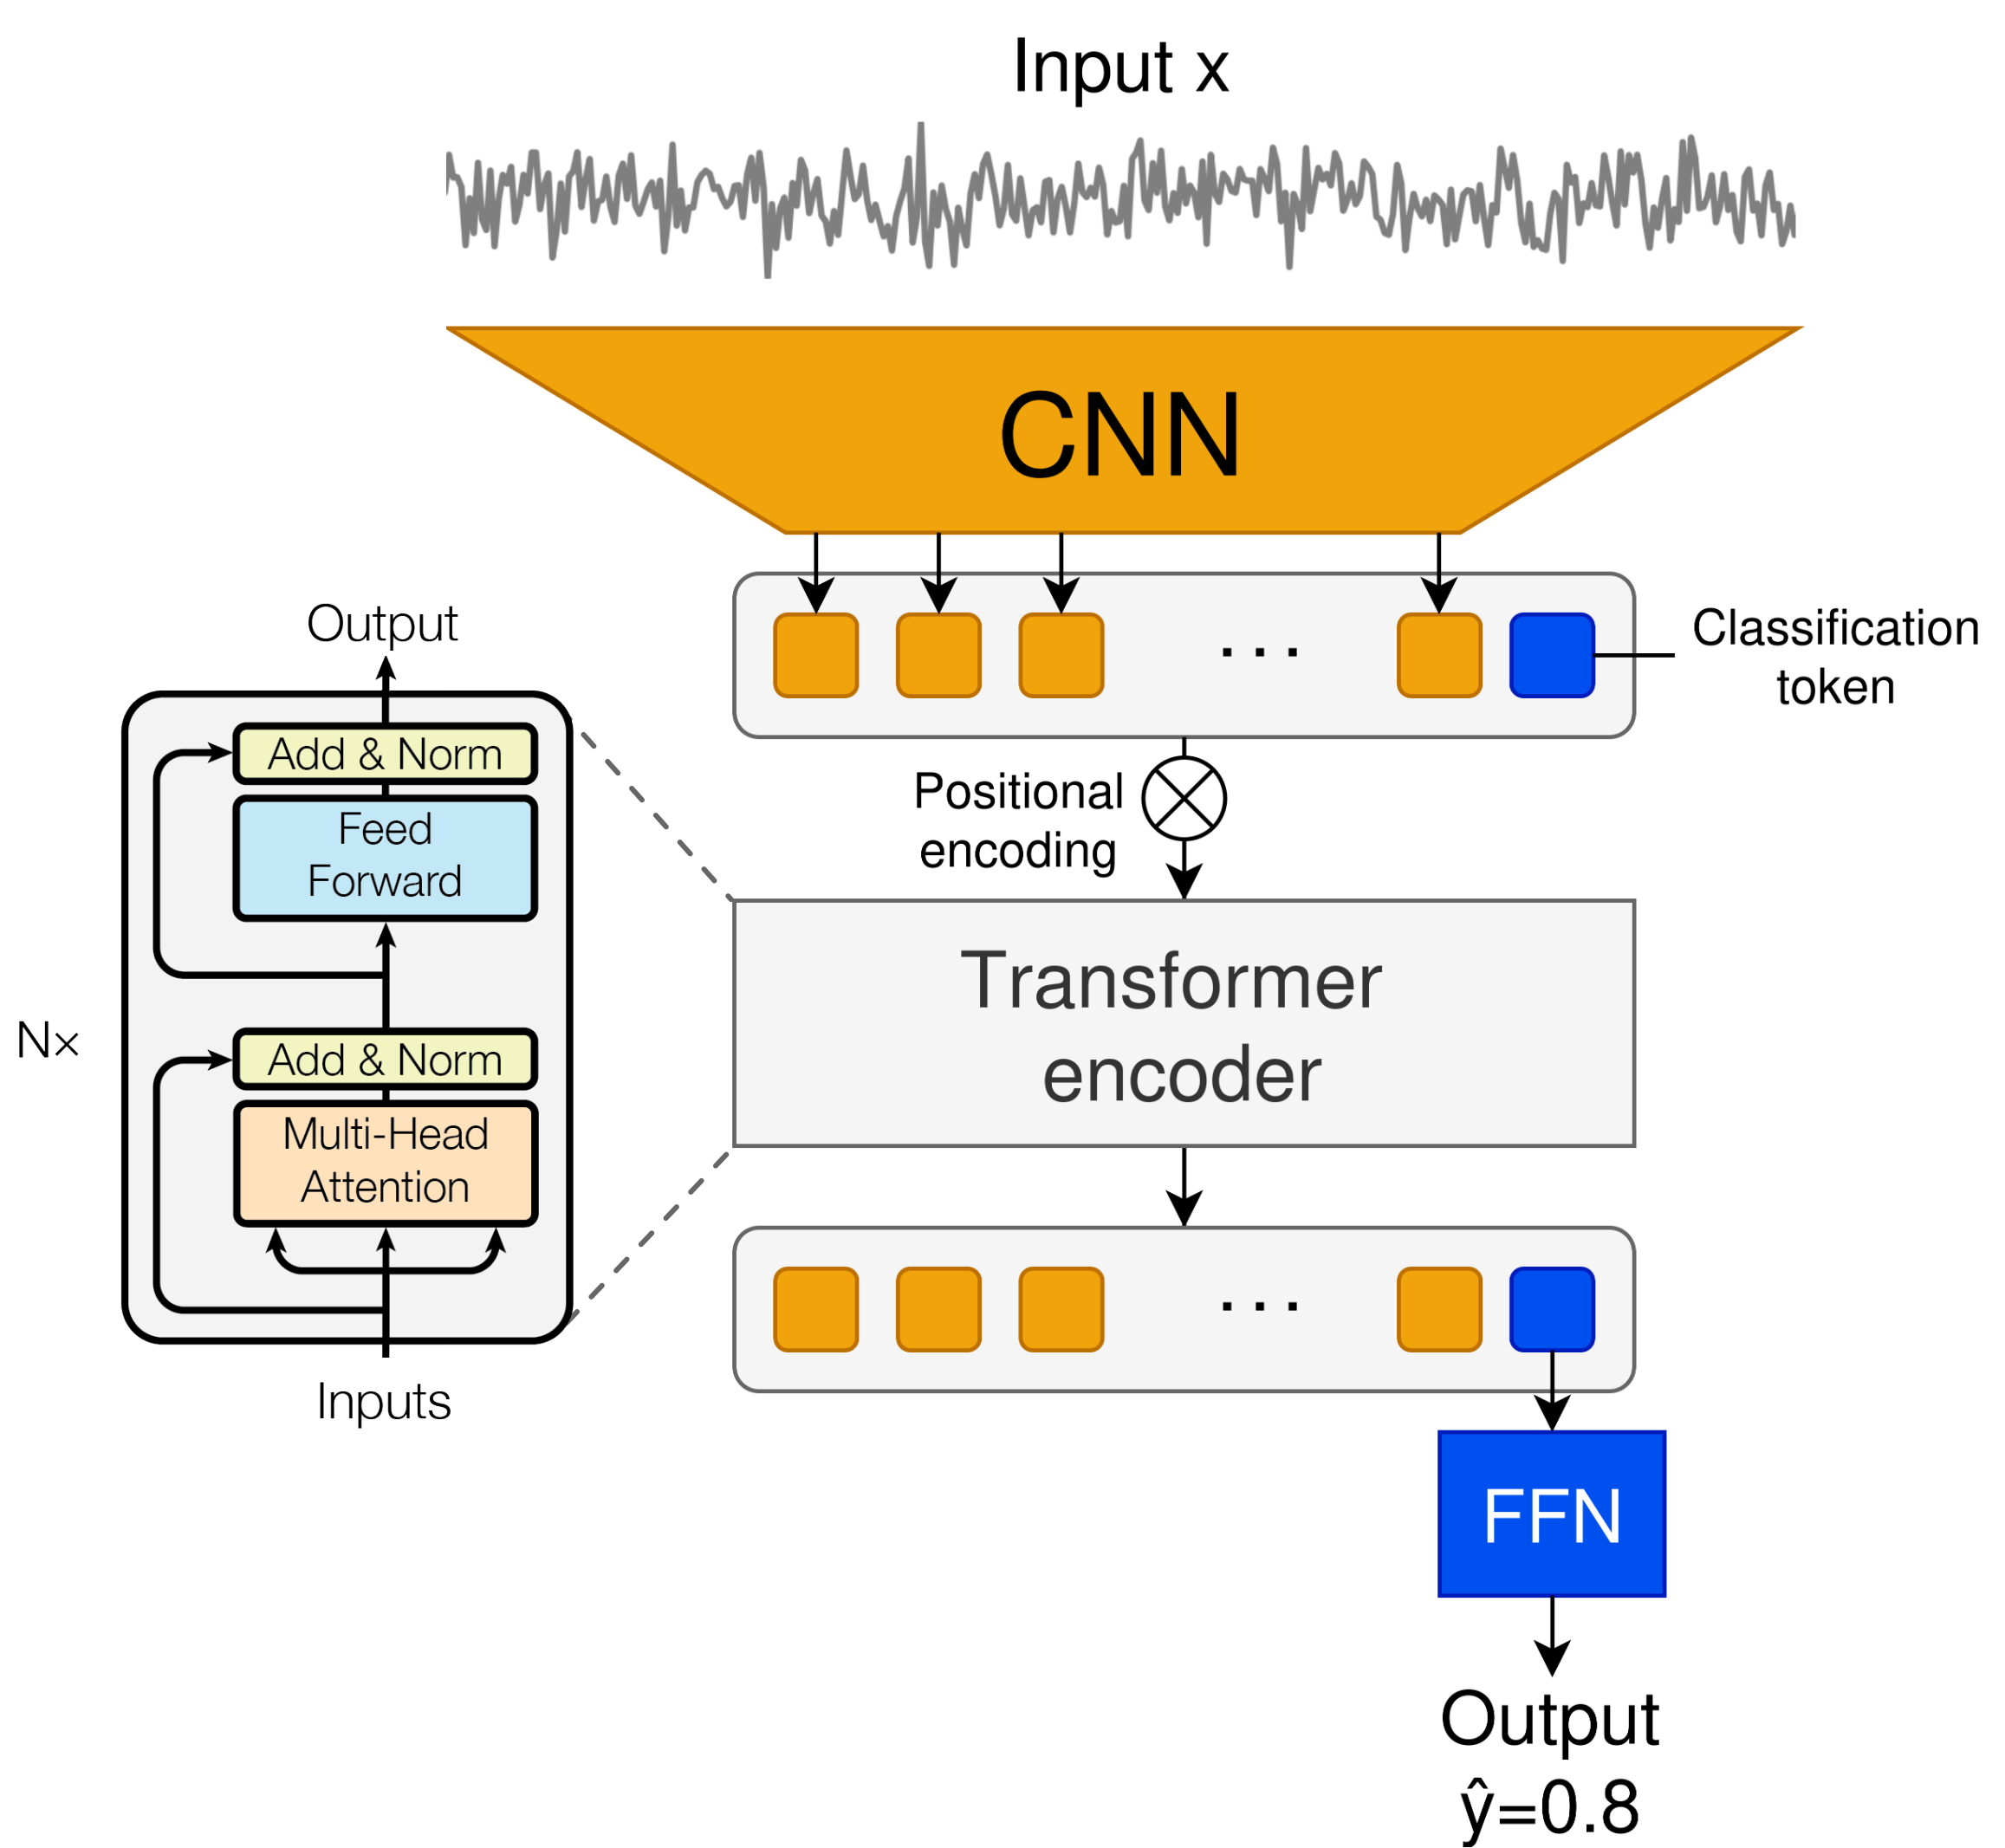
\includegraphics[width=11cm]{binary_classification/images/vit}
	}
	\caption{ViT architecture with an extra classification token.}
	\label{fig:binary:cnn_plus_vit}
\end{figure}

The transformer model, on the other hand, is implemented similarly to the \emph{Vision Transformer} (ViT) \cite{dosovitskiy2021an}, which was originally developed for image classification. The model makes use of the transformer encoder only, which takes as input a number of tokens which are somehow obtained from the input data. The ViT architecture appends an extra learnable \emph{classification token}. This token can attend to the input sequence through the transformer's attention mechanism and its output is read out via a classification head to yield a single class score. See a schematic of the architecture in Fig.~\ref{fig:binary:cnn_plus_vit}.

In NLP, sentences can be straightforwardly tokenized into single words. For other sequential data, appropriate tokenization is less obvious, and there are multiple ways to achieve it. The original ViT model tokenizes 2D images, by splitting them into patches and projecting these onto the desired embedding dimension. For GW data, initial tests showed that this tokenization scheme is too primitive, and results in bad performance. Instead, this work opts for a hybrid approach, where a full CNN serves as the tokenizer. This is outlined in \cite{dosovitskiy2021an} as well, and a similar approach is implemented for transformer based parameter estimation of overlapping signals \cite{Papalini_2025}.
For this CNN tokenizer, the same ResNet model which is described above is employed without average pooling and the classification head. 
For the largest considered input size, this yields $512$ tokens with $256$ channels. 
The resulting tokens represent the input time series in a time-ordered manner, downsampled by a factor of $256$. Each token carries the information of $\approx\SI{1}{\second}$ of data, corresponding to the CNN receptive field size.
A convolution operation with kernel size one reduces the number of channels to the desired embedding dimension $d_\text{embed}=64$.

The classification token is a vector of the same dimension, consisting of learnable parameters. These are initialized randomly. Following \cite{dosovitskiy2021an}, instead of fixed sinusoidal positional encodings, learned position embeddings are added to the input tokens. These are initialized randomly.
The transformer encoder comprises four layers, the attention blocks have eight heads each, and the dense networks' hidden dimension is of size $1024$. The final classification head reads, 
%\begin{equation}
%	z = \text{Dropout}(\text{Linear}_{1024\rightarrow1}(\text{ReLU}(\text{Dropout}(\text{Linear}_{64\rightarrow1024}(\text{LayerNorm}(x)))))),
%\end{equation}
\begin{equation}
\begin{aligned}
	n &= \mathrm{LayerNorm}(x),\\
	h &= \mathrm{Dropout}(\mathrm{ReLU}(\mathrm{Linear}_{64\rightarrow1024}(n))),\\
	z &= \mathrm{Dropout}(\mathrm{Linear}_{1024\rightarrow1}(h)),
\end{aligned}
\end{equation}
which is passed through a sigmoid activation later.
The model employs a dropout probability of \SI{10}{\percent}. (It should be noted that adding a final dropout layer to the classification head is uncommon and unintentional. The results will show that this does not hinder performance, although it leads to unusual learning curves.) The total model size is \SI{1.7}{\mega\nothing} learnable parameters. Apart from the learned embeddings, this is again independent of the input size.

\section{Training}

% minimize bce loss 
% mention logits for numerical stability

As is standard for binary classification tasks, the models are optimized by minimization of the \emph{binary cross entropy} (BCE) loss. Denoting the model output $\hat{y}$ and the target label $y$, this reads,
%\begin{equation}
%	\pazocal{L}_\text{BCE}(y,\hat{y}) = -(y\log{\hat{y}} + (1-y)\log{(1-\hat{y})}).
%\end{equation}
\begin{equation}
	\pazocal{L}_\text{BCE}(y,\hat{y}) = \begin{cases}
		-\log{(1-\hat{y})} & \text{if $y=0$,} \\
		-\log{\hat{y}} & \text{if $y=1$.} 
	\end{cases}
\end{equation}
In practice, the BCE loss is computed directly from the model \emph{logits} $z$ instead, \emph{i.e.}, the unbounded pre-sigmoid outputs, with $\hat{y} = \text{Sigmoid}(z)$. This ensures numerical stability. 

% dataset description 1m train validation with 0.9, 0.1 split and 131k test samples
% even dataset, i.e. 50% positive and 50% negative samples

% optimizer learning rate of 10^-4 batchsize 64
% maximum 100 epochs
% choose weight decay such that models do not overfit drastically

Training datasets are split into \SI{90}{\percent} train and \SI{10}{\percent} validation subsets. Models are trained for a maximum of 100 epochs with the \emph{AdamW} optimizer \cite{loshchilov2019decoupledweightdecayregularization} with a learning rate of \SI{E-4}{}.
The optimizer employs a relatively high weight decay of \SI{0.1}{} to hinder overfitting.
The batch size is $64$, thus each epoch comprises \SI{15}{\kilo\nothing} steps.

% lr scheduler
% CNN: reduce on plateau (similar to magic bullet paper)
% cosine annealing with warmup, standard for transformer architectures

This work utilizes different learning-rate schedules for the two model architectures.
When training the CNN, the learning rate is reduced by a factor of \SI{10}{} if the validation loss has not decreased by at least \SI{0.01}{} in the last 15 epochs. This is similar to \cite{PhysRevD.100.063015}. The ViT is trained with a cosine-annealing learning-rate schedule~\cite{loshchilov2016sgdr}. This is commonly used for transformer architectures. In this case, the learning rate is adjusted by a factor $\alpha$, which depends on the current training epoch and step $x$,
\begin{equation}
	\alpha(x) = \begin{cases}
		\frac{x}{x_0} & x\in[0,x_0), \\
		\frac{1}{2}(1+\cos{\pi\frac{x-x_0}{x_\text{max}-x_0}}) & x\in[x_0,x_\text{max}), \\
		0 & \text{else}.
	\end{cases}
\end{equation}
The schedule yields a linear increase up to $\alpha=1$ at $x_0$, after which $\alpha$ slowly tapers off to zero at $x_\text{max}$. The values $x_0$ and $x_\text{max}$ are set to 2000 steps and 100 epochs respectively.

\begin{figure}
	\centering
	\makebox[\textwidth]{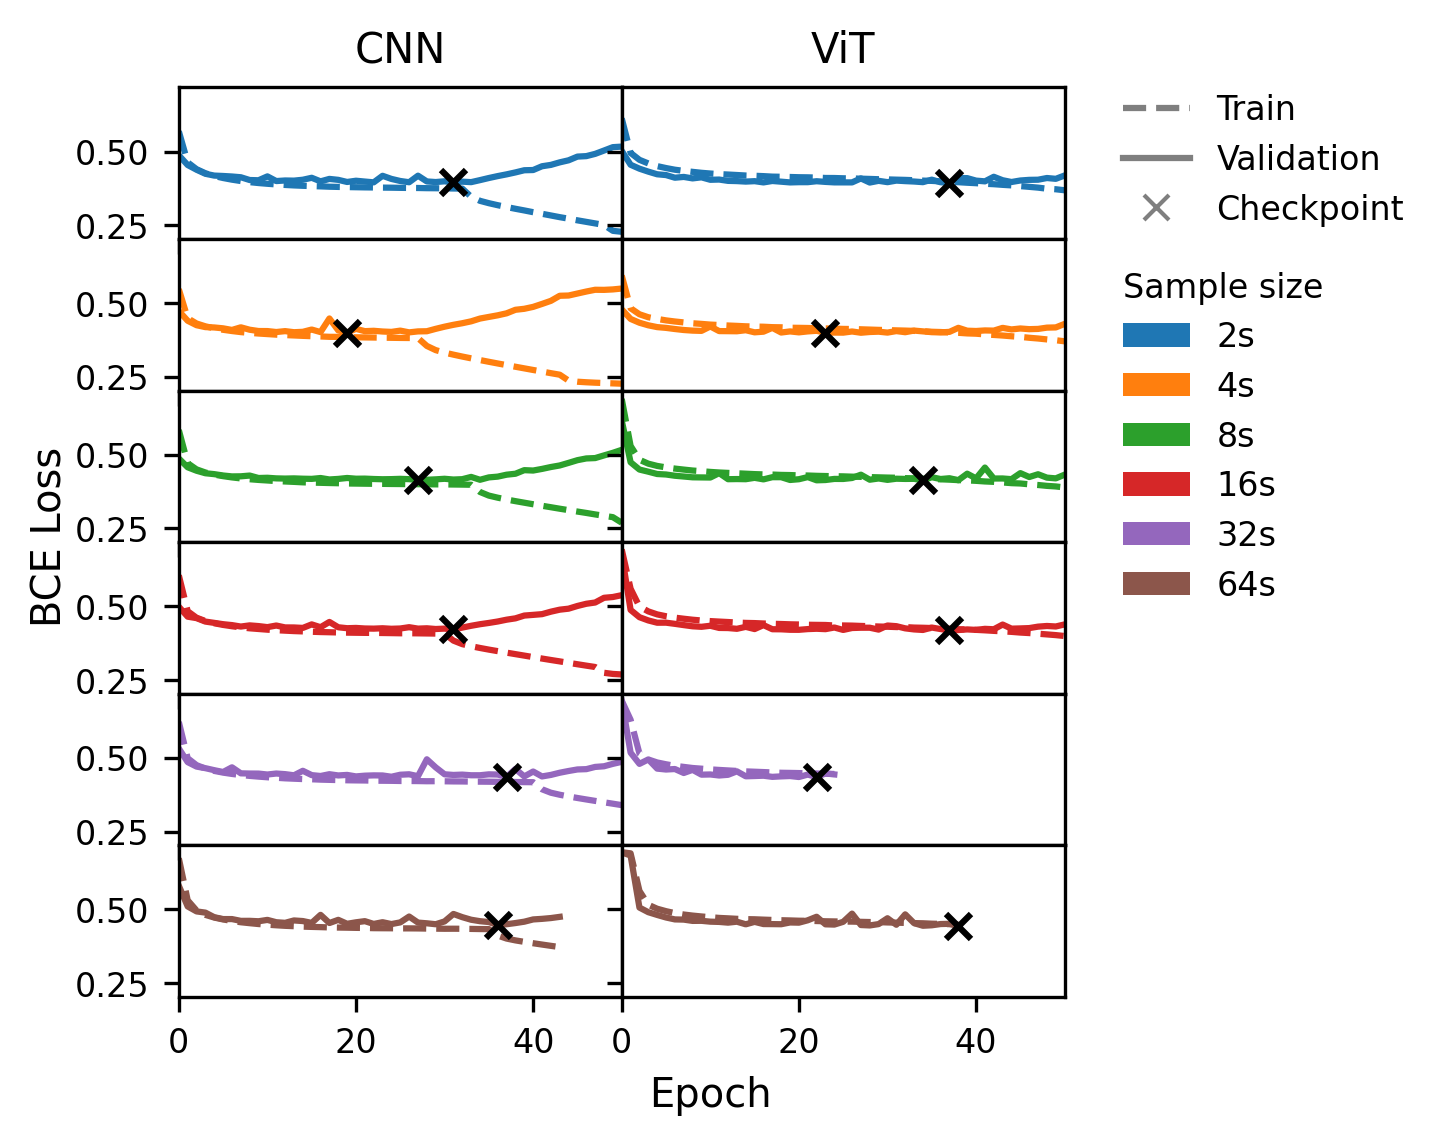
\includegraphics[width=12cm]{binary_classification/plots/learning_curves/curves}}
	\caption{Learning curves. Evolution of the BCE train (\emph{line}) and validation loss (\emph{dashed}) with training epoch for the CNN (\emph{left column}) and ViT models (\emph{right column}). Each row corresponds to one dataset with a different sample size. A marker denotes the minimum validation loss, the point after which overfitting occurs.}
	\label{fig:binary:learning_curves}
\end{figure}

% see learning curves
% all models start to overfit between 20 and 40 epochs
% both cnn and vit have enough parameters for this task
% difference in performance can be interpreted as being caused by model architecture

See the learning curves of all models and datasets plotted in Fig.~\ref{fig:binary:learning_curves}. It can be seen that both the CNN and ViT models start to overfit between 20 and 40 epochs. From this, it can be concluded that both models have enough parameters for this task. Apart from the different learning schedules, differences in performance can be attributed to model architecture only. (Note that, surprisingly, for ViT, the validation loss is in fact smaller than the training loss in the early epochs. This is caused by the unintended final dropout layer, which randomly zeroes the model output with a probability of \SI{10}{\percent}. Since dropout is only applied during training and disabled for evaluation, the model performs better on the validation dataset.)

\section{Performance Comparison}

\begin{figure}
	\centering
	\begin{minipage}[t]{7.5cm}
		\centering
		\makebox[\textwidth]{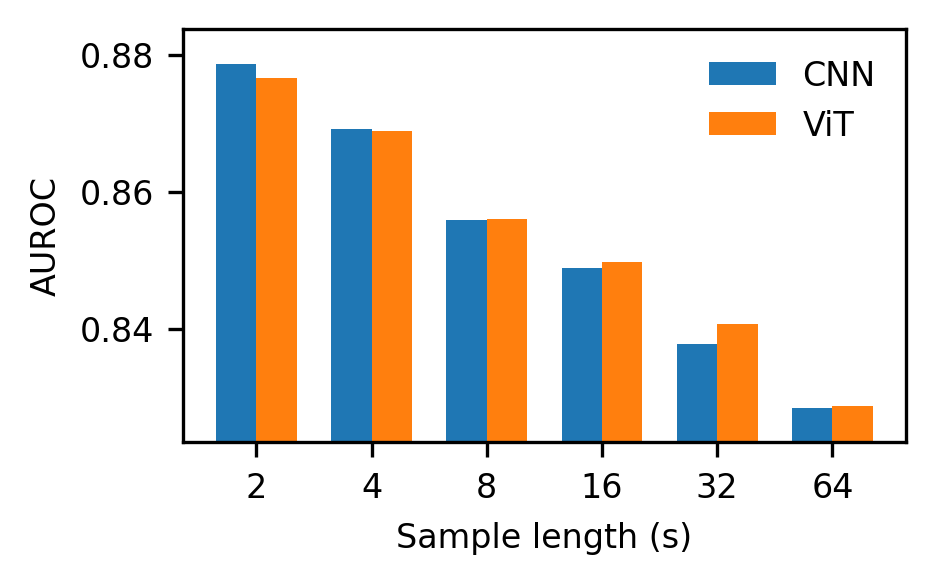
\includegraphics[width=8cm]{binary_classification/plots/comparison/performance}}
		\captionof{figure}{Test dataset AUROC for both models with respect to sample length. Computed over \SI{131}{\kilo\nothing} samples each.}
		\label{fig:binary:comparison}
	\end{minipage}
	\hfill
	\begin{minipage}[t]{7.5cm}
		\centering
		\makebox[\textwidth]{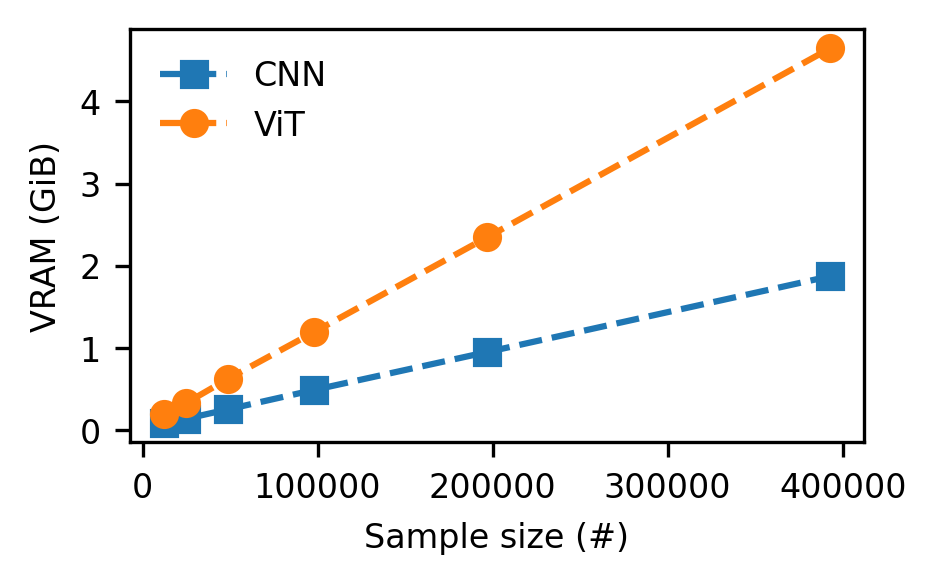
\includegraphics[width=8cm]{binary_classification/images/comparison/vram_size}}
		\captionof{figure}{Peak training VRAM usage with input size. Measured for 64 sample batches on an RTX 4090.}
		\label{fig:binary:vram}
	\end{minipage}
\end{figure}

% checkpointing: choose model parameters with lowest validation loss
% compute roc scores (see fig)
% model performance degrades with larger inputs (expected?)
% CNN and ViT perform equally well 

The performance of both models with respect to dataset sample length is compared. Each model's parameters are chosen from the checkpoint with the lowest validation loss (see Fig.~\ref{fig:binary:learning_curves}). The AUROC is computed over the \SI{131}{\kilo\nothing} sample test datasets, and plotted in Fig.~\ref{fig:binary:comparison}. 

Both models reach $\approx\SI{88}{\percent}$ AUROC for the shortest input size of \SI{2}{\second}. Performance decreases to $\approx\SI{83}{\percent}$ AUROC for \SI{64}{\second}. This decrease was expected and may be attributed to all training datasets having the same size of \SI{1}{\mega\nothing} samples regardless of sample length. The increased size adds complexity, necessitating more training samples.

It can be seen that both the CNN and ViT perform equally well. Contrary to the hypothesis that the attention mechanism handles large inputs more efficiently, this concludes that transformers introduce no performance gain in this context. 
% Still, the transformer architecture achieves comparable performance. 
Although its memory usage is higher compared to the CNN, with at most 512 tokens for \SI{64}{\second} samples, it is far from the quadratic regime expected from the attention mechanism (see Fig.~\ref{fig:binary:vram}). This is an important intermediate result before dealing with overlapping signals.

\section{Parameter Biases}

% look at performance on 64s samples for one model (vit) more closely
% check for biases (from dataset)
% diagnostic check

Having established that both models can process the desired input size, the performance of the ViT model on \SI{64}{\second} samples is studied in more detail.  The goal is to perform diagnostic checks before moving to overlapping waveforms. In particular, these are checks for any biases the model might have learned with respect to the injected waveform's parameters. Since both models perform similarly, the assumption is made that biases mostly depend on the data itself and not the model type. The ViT model is chosen for this analysis because its attention weights provide an additional diagnostic of which parts of the input contribute to the classification.

% choose arbitrary threshold 
% see roc curve
% minimize distance to (FPR=0, TPR=1)

\begin{figure}
	\centering
	\makebox[\textwidth]{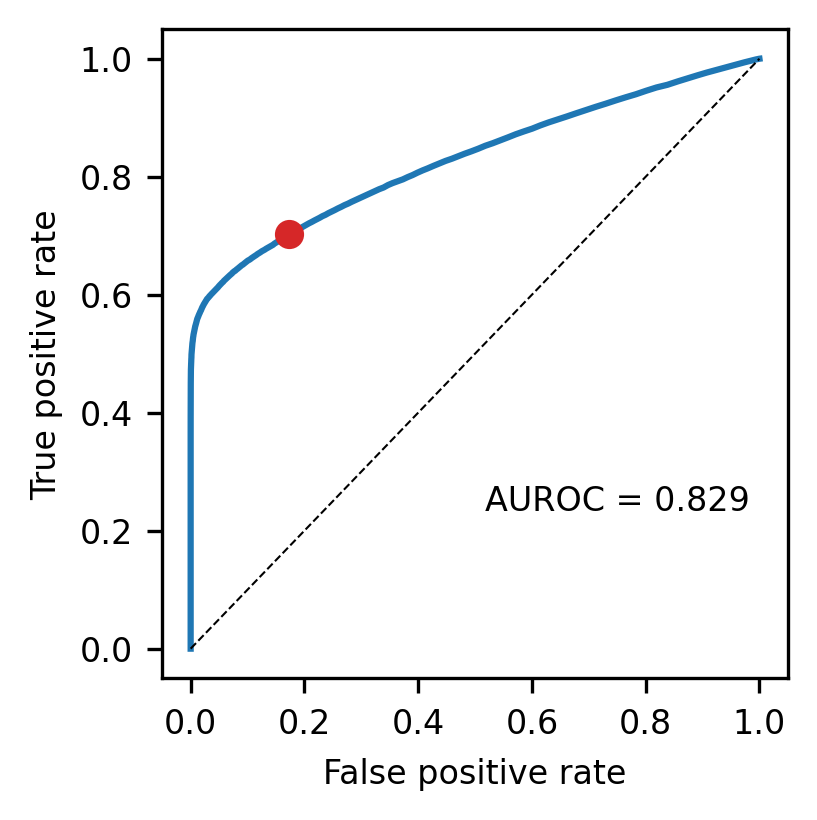
\includegraphics[width=7cm]{binary_classification/plots/auroc}}
	\caption{ViT ROC for \SI{64}{\second} samples. The dotted line shows the performance of a random classifier, which has \SI{50}{\percent} AUROC. The red dot shows the chosen operating point.}
	\label{fig:binary:auroc}
\end{figure}

Employing this model as a binary classifier requires choosing an appropriate \emph{operating point} first. This means setting the threshold to yield some FPR and TPR. To this end, the ROC is consulted in Fig.~\ref{fig:binary:auroc}, which shows all the possible operating points. Note that there are many points with a FPR close to zero while reaching TPR up to $\approx\SI{50}{\percent}$. This reveals that a large fraction of target positive samples are easy to identify for the network. This is promising for GW searches, which focus on minimizing the false alarm rate while reporting as many signals as possible.

Again, as this study does not aim to implement a proper search, and is interested in diagnostic checks for now, the operating point can be chosen more or less arbitrarily. One such way is to find the threshold such that the resulting operating point has minimum distance to a perfect classifier with zero FPR and unit TPR. Then, the desired or optimal threshold is,
\begin{equation}
	z_\text{opt} = \argmin_{z} \sqrt{\text{FPR}(z)^2 + (1-\text{TPR}(z))^2},
\end{equation}
resulting in a threshold of \SI{27.5}{\percent}. Model predictions below \SI{27.5}{\percent} are labeled negative and positive else. This gives \SI{17.4}{\percent} FPR and \SI{70.2}{\percent} TPR. \SI{17.4}{\percent} of all noise samples are incorrectly predicted to contain a signal, and \SI{70.2}{\percent} of all injection samples are correctly identified. 
% See the confusion matrix in Fig.~\ref{fig:}.

% explain detection ratio 

The metric by which the model's performance with respect to the waveform parameters is evaluated is the \emph{detection ratio}. That is, how many signals (which have these waveform parameters) are found? In this case, this is simply the TPR. 

\begin{figure}
\centering
\begin{subfigure}{0.48\textwidth}
	\centering
	\makebox[\textwidth]{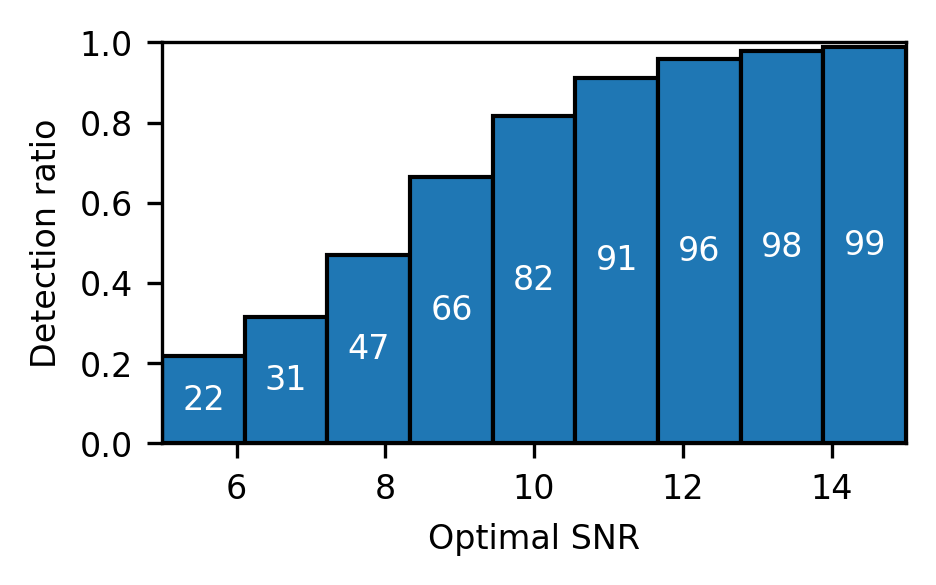
\includegraphics[width=8cm]{binary_classification/plots/snr}}
	\caption{}
	\label{fig:binary:snr}
\end{subfigure}
\hfill
\begin{subfigure}{0.48\textwidth}
	\centering
	\makebox[\textwidth]{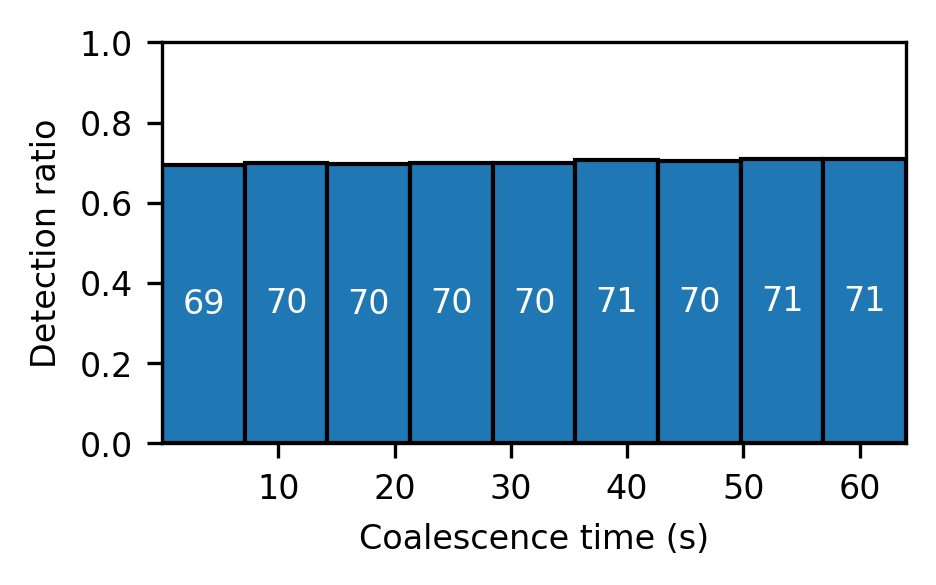
\includegraphics[width=8cm]{binary_classification/plots/merger_time}}
	\caption{}
	\label{fig:binary:merger_time}
\end{subfigure}
\begin{subfigure}{0.48\textwidth}
	\centering
	\makebox[\textwidth]{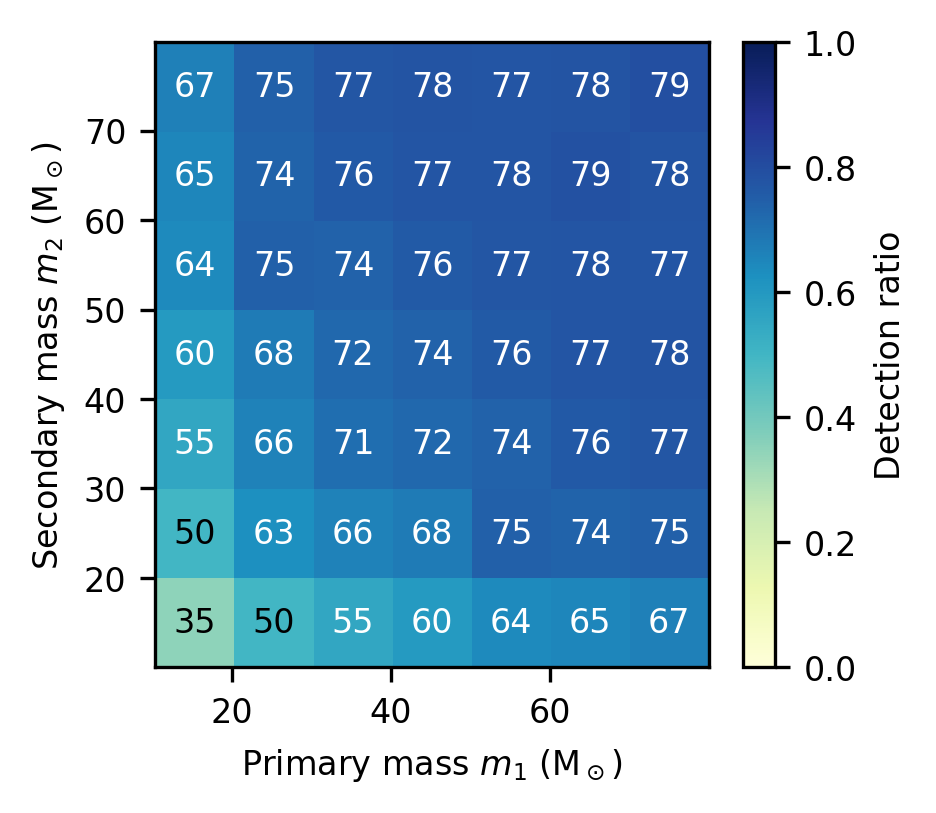
\includegraphics[width=8cm]{binary_classification/plots/mass}}
	\caption{}
	\label{fig:binary:mass}
\end{subfigure}
\hfill
\begin{subfigure}{0.48\textwidth}
	\centering
	\makebox[\textwidth]{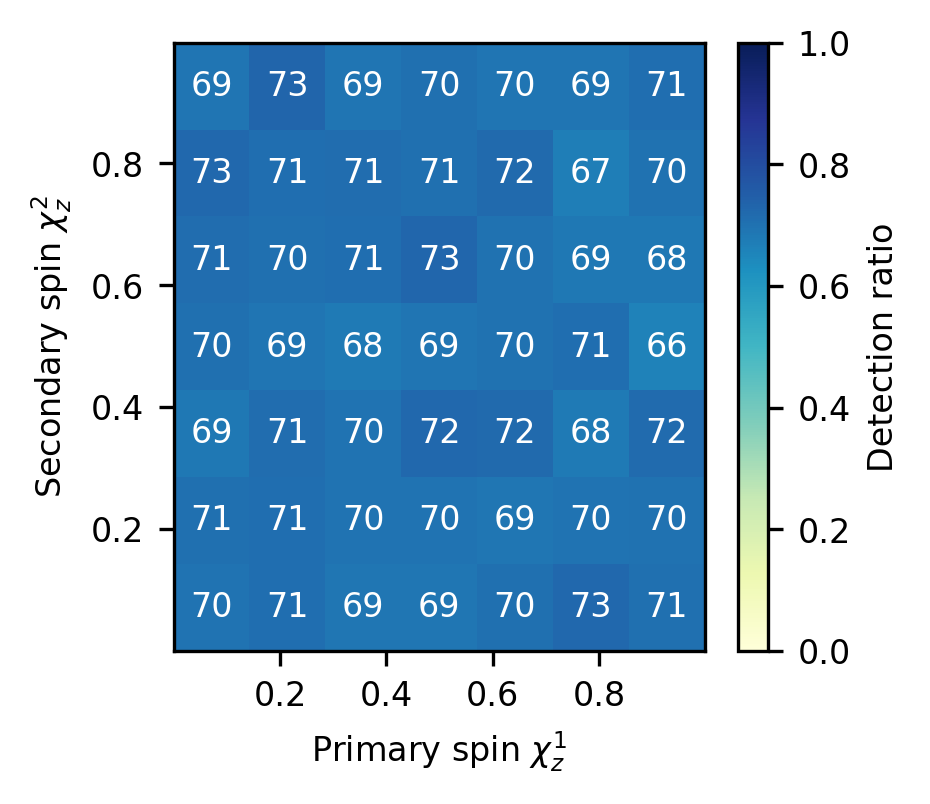
\includegraphics[width=8cm]{binary_classification/plots/spins}}
	\caption{}
	\label{fig:binary:spin}
\end{subfigure}
\caption{Detection ratio as a function of various signal parameters: SNR (\emph{a}), coalescence time (\emph{b}), the two objects masses (\emph{c}) and spins (\emph{d}). Computed over a total of \SI{66}{\kilo\nothing} test samples. In (\emph{c}), the values are mirrored along the diagonal for visualization purposes. Labels are rounded to the nearest integer or the first decimal place. Uncertainties are not plotted.}
\end{figure}

% snr plot
% detection ratio increases with snr
% expected
% good because it verifies that the models really learn to identify GW signals instead of picking up on some giveaways caused by faulty data

It is natural to first consider the model's performance with respect to SNR. Test samples are subdivided into nine SNR bins in $[5, 15]$, and the detection ratio is computed separately for each bin. The result is shown in Fig.~\ref{fig:binary:snr}. In this case, half of the test dataset is considered consisting of only positive samples containing a signal. Thus, each bin consists approximately $N=\SI{7}{\kilo\nothing}$ test samples. Assuming a binomial distribution with probability $p$, \emph{i.e.}, the detection ratio, then each bin has a standard deviation of $\sigma = \sqrt{p(1-p)/N}$.

It can be seen that the model achieves close to perfect detection ratios of \SI{99.0(1)}{\percent} for the loudest signals, indicating that these signals are easily identified. For the faintest signals, the detection ratio decreases to \SI{21.7(5)}{\percent}. This trend is expected: low-SNR signals are harder to distinguish from noise. It is also a useful sanity check, since it suggests that the network output is correlated with the signal loudness rather than with any artefacts in the simulated data.

% merger time plot
% detection ratios only varies slightly with merger time
% no biases with merger time 
% slight decrease for mergers closer to 0, because less of their signal lies in the sample (check significance)
% 9 bins, 131k/9 samples per bin, sigma = sqrt(0.7(1-0.7)/(131k/9)) = 0.4%

The same analysis is applied to the signal coalescence time, i.e. the position of the merger within the sample. See the results in Fig.~\ref{fig:binary:merger_time}. The network achieves detection ratios $\approx\SI{70}{\percent}$ regardless of coalescence times. A small decrease is noticeable from $\SI{71.0(5)}{\percent}$ for signals whose merger lies close to the \emph{right} sample edge down to $\SI{69.4(5)}{\percent}$ closer to the \emph{left} edge. A decrease is expected, since less of the signal inspiral phase is contained in the sample in this case. Here, the effect is statistically insignificant, suggesting that predictions are made mostly based on the signals' late inspiral and merger phase, rather than by the full waveform.

% mass plot
% detection ratio decreases with lower mass
% more snr lies in the inspiral for low mass inspirals (see plot)
% maybe network only focuses on merger? check attention weights

Because the shape of CBC waveforms depends largely on the component masses $m_1, m_2$ (compare Eq.~\ref{eq:gravitational_waves:cbc_waveform}), it makes sense to investigate model performance as a function of these. To this end, both the primary and secondary masses are subdivided into seven bins in $[\SI{10}{\solarmass}, \SI{80}{\solarmass}]$. From this, a $7\times7$ matrix is constructed with rows corresponding to the primary mass $m_1$ bins and columns to the secondary mass $m_2$ bins. The detection ratio is computed separately for each entry. Since $m_1>m_2$, the upper triangular half of that matrix contains no samples. To yield a full matrix, entries are mirrored along the diagonal. The result is plotted in Fig.~\ref{fig:binary:mass}.

The plot exhibits two notable features, which are both statistically significant. First, the detection ratio increases with total mass, from $\SI{35(1)}{\percent}$ for the lowest total masses $M = m_1+m_2 \approx\SI{20}{\solarmass}$ up to $\SI{79(1)}{\percent}$ for the highest masses $\approx\SI{160}{\solarmass}$. Second, along diagonals of approximately constant total mass, the detection ratio decreases with \emph{mass ratio} $q = m_1 / m_2$. For example, along the center diagonal with total mass $M \approx \SI{90}{\solarmass}$, the detection ratio decreases from $\SI{74(1)}{\percent}$ for equal masses, \emph{i.e.}, $q\approx1$ to $\SI{66.5(9)}{\percent}$ for mass ratios close to $q\approx8$.

\begin{figure}
	\centering
	\makebox[\textwidth]{
		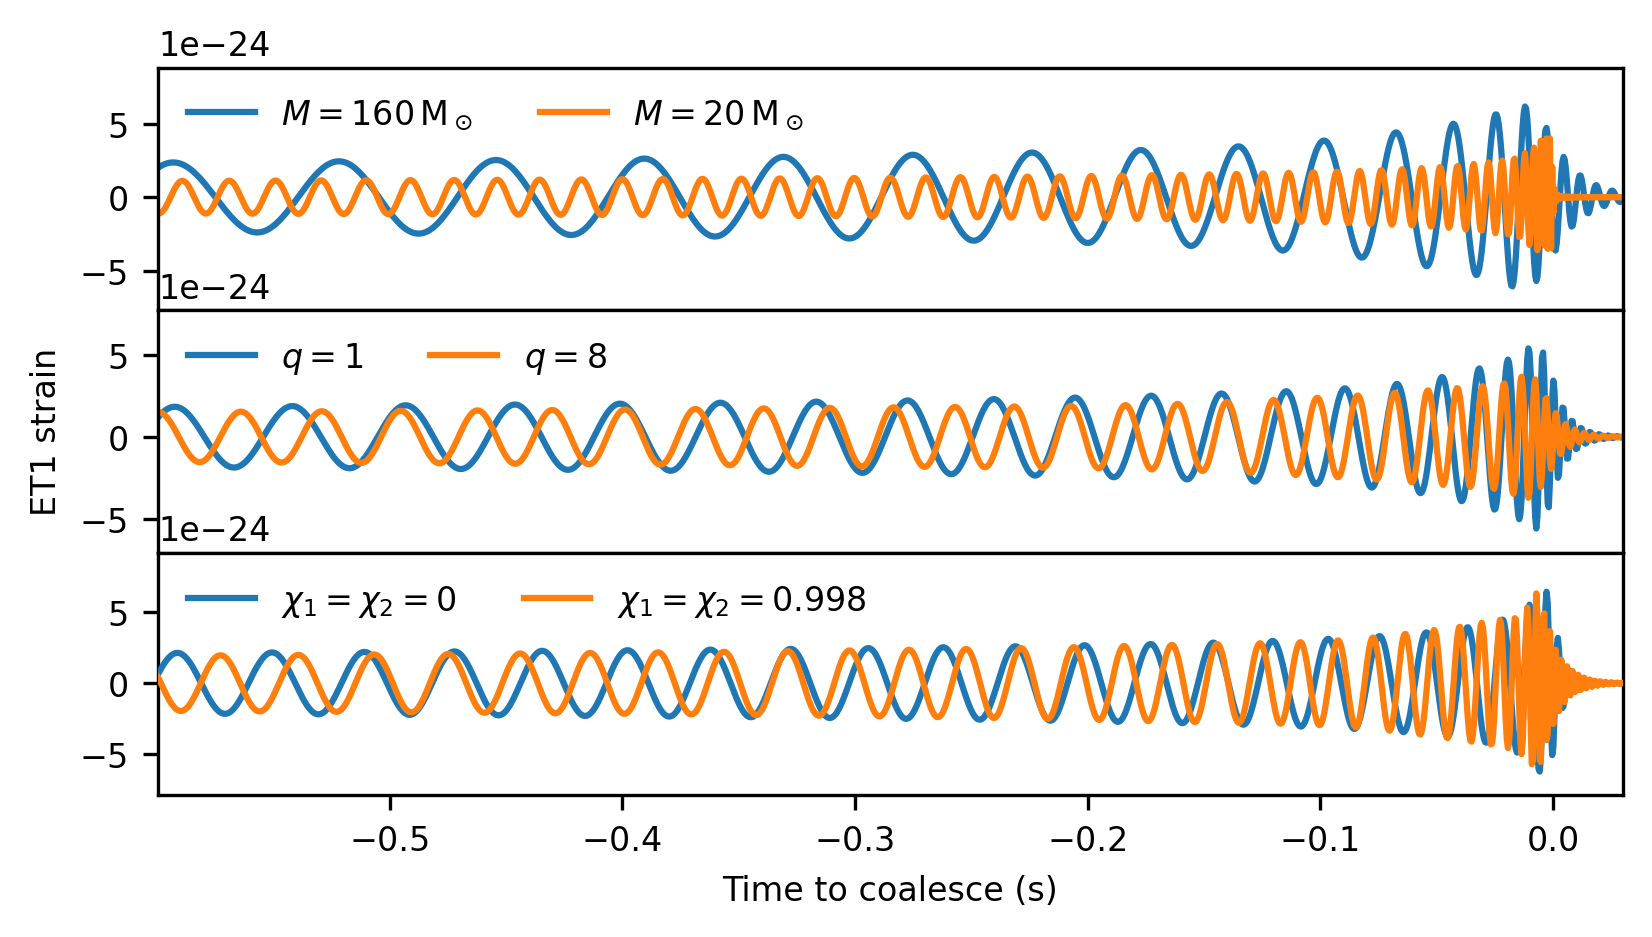
\includegraphics[width=16cm]{binary_classification/images/parameters/waveforms}
	}
	\caption{Equal-SNR ($\rho=10$) signals with different parameters. For visualization purposes, only the ET1 channel is plotted. Each row shows two waveforms with different total mass (\emph{top}), mass ratio (\emph{middle}), and spins (\emph{bottom}) and otherwise equal parameters.}
	\label{fig:binary:low_mass_waveform}
\end{figure}

Both effects can be understood from the dependence of the waveform duration on chirp mass. At leading order, the duration scales as $\tau \propto 1/\pazocal{M}^\frac{5}{3}$ (see Eq.~\ref{eq:matched_filtering:signal_duration}).
The chirp mass can be written as
\begin{equation}
	\pazocal{M} = \frac{(m_1m_2)^\frac{3}{5}}{(m_1+m_2)^\frac{1}{5}} = \frac{q^\frac{3}{5}}{(1+q)^\frac{6}{5}}\,M.
\end{equation}
Therefore, lower total masses and larger mass ratios correspond to smaller chirp masses and hence longer signals. The observed decrease in detection ratio can thus be interpreted as a degradation of model performance for longer-duration signals. 

For these longer waveforms, SNR lies mostly in the long inspiral phase. If two signals have equal SNR, but one is longer, the longer waveform will have a smaller total amplitude. See Fig.~\ref{fig:binary:low_mass_waveform} where equal-SNR waveforms with different masses are compared. 
Assuming sufficient template size, matched filtering detects these signals equally well, regardless of signal amplitude, since their SNR is the same. For neural networks, however, longer and lower-amplitude signals appear to be more challenging.

% spin plot
% 7^2 bins, 131k/7^2 samples per bin, sigma = sqrt(0.7(1-0.7)/(131k/7^2)) = 0.9%
% no biases -> good

Finally, the detection ratio is checked against the remaining intrinsic waveform parameter, each black hole's spin z-component. Remember that only aligned-spin BBHs are considered in this work, which have vanishing spin x and y-components. Similar to the mass analysis, the primary and secondary spins are subdivided into seven bins in $[0,0.998]$, forming a $7\times7$ matrix. Since the spin values are drawn independently, each entry contains \SI{2400}{\nothing} samples. The result is plotted in Fig.~\ref{fig:binary:spin}. A detection ratio of $\approx\SI{70}{\percent}$ is achieved throughout. No clear trend is visible, and values vary between \SI{66.1(1.3)}{\percent} and \SI{72.9(1.2)}{\percent}, which is a difference of $3.8\,\sigma$. Thus it can be concluded that model performance is agnostic to the binary component spins. This is consistent with the earlier result that performance is mostly limited by signal length and amplitude. By simulating equal-SNR waveforms with different spins (see Fig.~\ref{fig:binary:low_mass_waveform}), it can be seen that, contrary to the effect of different component masses, the waveforms vary very little with spin.
 
\section{Attention Analysis}

Up to now, the results suggest that the neural network makes predictions mostly based on the waveform's merger phase where the amplitude is maximum. Because of this, performance is independent of injection time, but degrades for longer waveforms where most of the SNR lies in the inspiral part. As this analysis uses the ViT model, this hypothesis can be validated by checking the model's attention weights.

% new 65k sample test dataset with fixed merger time at 60s to gather some statistics
% mean attention weights of classification token
% bin into snr ranges
% see plot

For this, a new test dataset is simulated with \SI{66}{\kilo\nothing} positive, \emph{i.e.}, signal containing, samples with constant coalescence time. The sample size is \SI{64}{\second} and signals are always injected with a coalescence time of \SI{60}{\second}. The simulation parameters are otherwise unchanged. 

To check what lead the ViT model to make its prediction, the transformer encoder weights are investigated. These correspond to a $513\times513$ self-attention matrix for the $512$ time series tokens and the extra classification token. Each row of this matrix corresponds to one target or output token, and each entry of that row contains the weight that token assigns to the source or input tokens. 

Since the final prediction only depends on the classification token, only the weights that this token assigns to the other $512$ time series tokens are of interest. These weights correspond to the first $512$ entries in the last row of the attention matrix. After CNN tokenization, the resulting tokens still represent the input series in a time ordered, albeit downsampled, fashion. Thus, the considered $512$ classification token attention weights can be related to the input time series to show which part of the waveform is deemed important for the prediction.

\begin{figure}
	\centering
	\makebox[\textwidth]{
		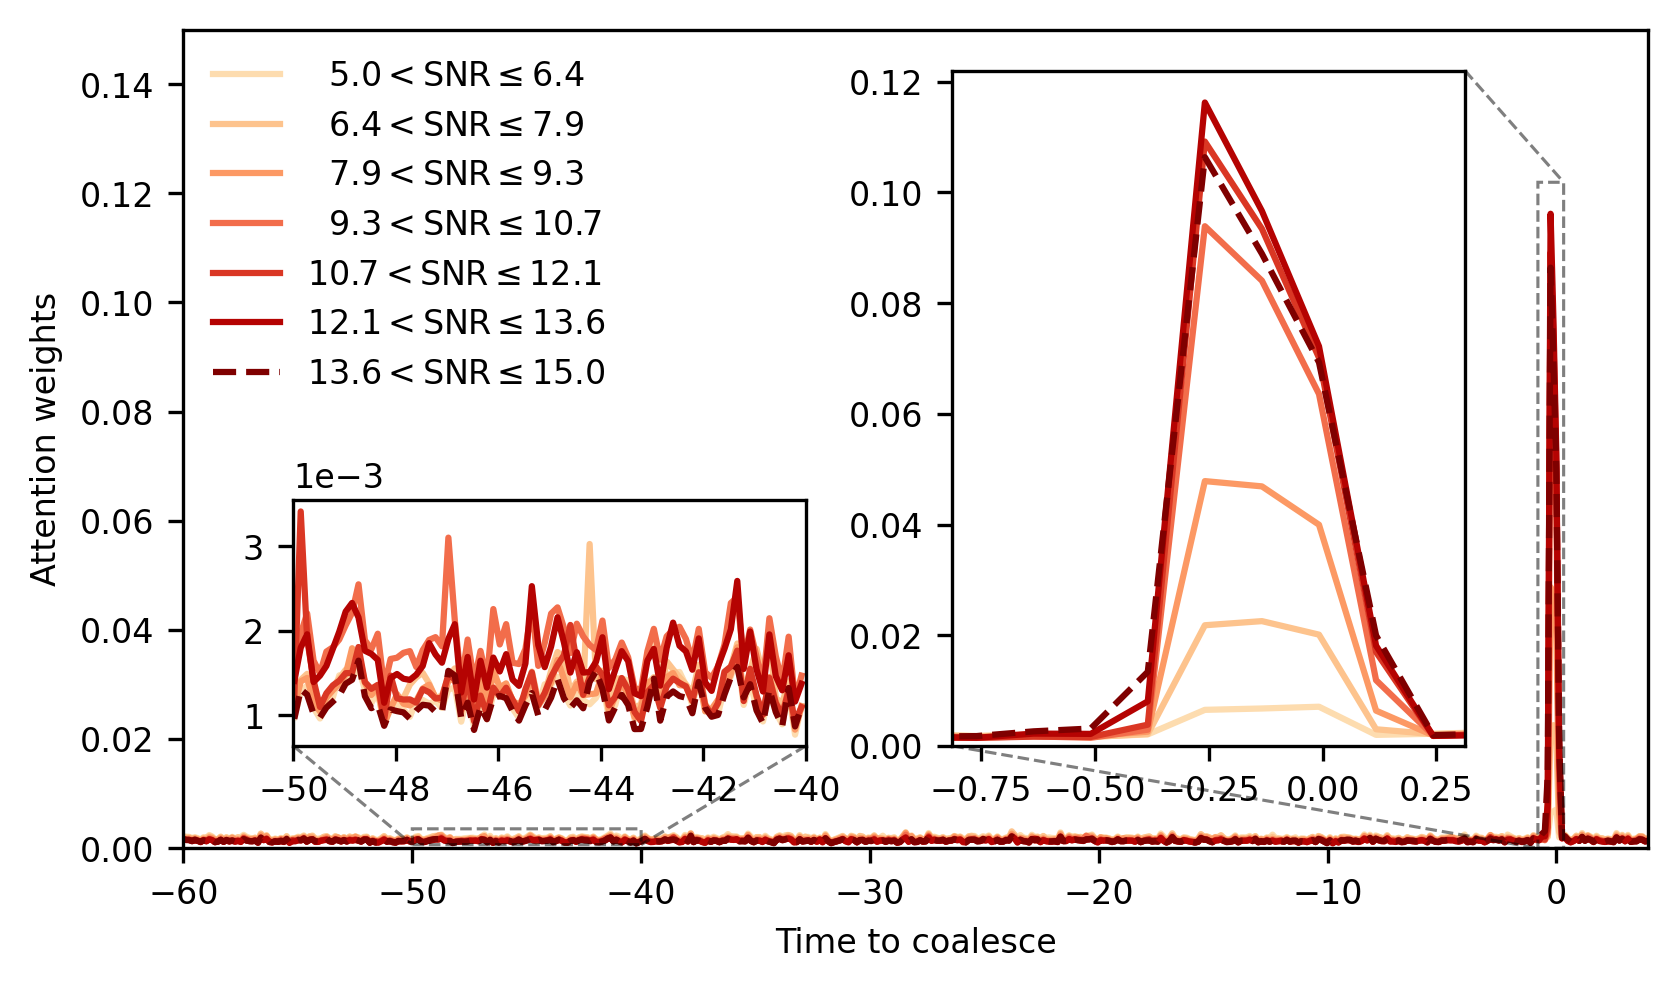
\includegraphics[width=16cm]{binary_classification/plots/attention/attention}
	}
	\caption{Attention weights assigned by the ViT classification token to the input time series tokens. Averaged over multiple samples with fixed merger time. Seven SNR bins are considered. The corresponding weights are plotted in different colors. Darker colors signify louder signals. The highest-SNR weights are dashed for clarity.}
	\label{fig:binary:attention}
\end{figure}

In particular, the last encoder layer's weights are investigated, and these averaged over all eight heads.
To gather some statistics, these weights are again averaged over multiple samples. To this end, the test dataset is divided into seven SNR bins in $[5, 15]$, each containing \SI{9}{\kilo\nothing} samples. For each subset, and for each timestep, the weights are the averaged separately. See the result in Fig.~\ref{fig:binary:attention}.

% on average, attention focuses only on the last 0.5s until merger
% peak increases in height with snr
% except for last bin where the peak gets slightly more broad, i.e. more of the waveform is payed attention to, but this effect is very minor

From this plot, it becomes clear that the attention is very \emph{sparse}. Most attention is paid to the $\approx\SI{1}{\second}$ around the merger, leaning more towards the inspiral instead of the ringdown phase. The height of that peak grows for louder signals, from $\approx\SI{E-2}{}$ for low SNRs up to  $\approx\SI{E-1}{}$ for high SNRs. Outside that region, the weights are smaller on average with values of order $\pazocal{O}(\SI{E-3}{})$. 

% verifies that attention mechanism works 
% again data is propably not faulty
% although large input size, network does not capture the waveform fully
% maybe increase performance by making attention less sparse?
% curriculum learning

This verifies that the model prediction is based mostly on the high amplitude merger phase of the signal. From this, it is clear that networks struggle with long-duration waveforms since their maximum amplitude is lower. Although the network is able to process the whole \SI{64}{\second} sample size, only a fraction of that information is used to make predictions. 

Again, the attention weights serve as a useful sanity check. It can be verified that the transformer is implemented correctly and that the attention mechanism works as expected. Further, the plot suggests that the network does not pick up on any possible artefacts in the data, and that predictions are based on the signal's merger phase.

\section{Summary}

This study shows that both the CNN and ViT models can process the required sample size of \SI{64}{\second}. A performance decrease is observed when going to larger inputs, which is attributed to training data size. No clear performance advantage of the transformer model is observed in this single-signal setting. Further analysis shows that models struggle for long-duration waveforms, such as low mass inspirals and high mass-ratio inspirals. Although the networks manage to process the full \SI{64}{\second} sample, they seem to focus mostly on the high amplitude merger phase, which is less pronounced in long signals.

% models decrease in performance with input size
% both cnn and vit can process long inputs
% no clear performance gain from attention mechanism
% no biases in dataset
% data not faulty
% vit focuses only on last part of merger neglecting the long inspiral
% performance decreases for low mass inspirals

\chapter{Heatmap Regression}
\label{sec:heatmap}
% so far only binary classification \cite{George_2018}
% how to adapt to data stream? 

So far, this work has only dealt with the simplified problem of detecting one signal per sample, which can be treated as a binary-classification task. It remains to adapt the models to perform a proper GW search. Such a search processes a data stream of arbitrary length and returns multiple GW candidates along with some confidence measure and their time location in that data.

% CNN Binary classifier + sliding window + postprocessing \cite{Sch_fer_2023}
% works for short LIGO-like signals where a small window suffices
% we need large receptive fields to capture waveforms fully ~1min
% but for large ET event rates the classifier will (almost) always spit out true
% final output becomes meaningless

One simple approach, followed by the models in \cite{Sch_fer_2023}, for example, utilizes overlapping sliding windows of $\pazocal{O}(\SI{1}{\second})$. The already trained binary classifier assigns each window a score, resulting in a \enquote{probability} time series in $[0,1]$. From this time series, a number of post-processing steps yield multiple GW candidates.

This method is suitable for second-generation detector conditions, where signals are short. However, in ET, signal waveforms are longer and thus, larger input sizes are required of $\approx\SI{1}{\minute}$. Further, ET's increased event rate means that these long-duration windows are almost always contaminated by some amount of signals. For example, a $\SI{64}{\second}$ sample will contain the merger of at least one signal with a probability $\approx\SI{87}{\percent}$ (see Fig.~\ref{fig:data_simulation:poisson}). Therefore, employing a classifier that was trained in Ch.~\ref{sec:long_duration} over sliding $\SI{64}{\second}$ windows, will return mostly positive labels, making the final output useless.

An alternative approach is formulated in \cite{PhysRevD.100.063015}. Here, instead of training the binary classifier separately beforehand, the network is trained to output a time series, which contains peaks corresponding to the signal coalescence times. These are then extracted through various post-processing steps to yield GW candidates. 
% In \cite{PhysRevD.100.063015}, this network is \emph{fully convolutional}, which means it can be feed an input of arbitrary size, completely foregoing the need for slicing up the detector data stream.
Although not stated as such in the original paper, this approach will be called \emph{heatmap regression} in this thesis because of its similarity to an existing machine learning technique \cite{tompson2014jointtrainingconvolutionalnetwork}. 

In \cite{PhysRevD.100.063015}, the network is trained with \SI{8}{\second} long samples containing one signal at most. In this work, models are trained on longer-duration samples of \SI{64}{\second} containing multiple signals. 
As transformer models have shown good performance for overlapping signals in parameter estimation \cite{Papalini_2025}, this chapter compares two models, one CNN based and the other transformer based. For this, minimal adjustments to the models in Ch.~\ref{sec:long_duration} are made, changing the task from binary classification to heatmap regression.

% \cite{PhysRevD.100.063015} train with 8s samples containing one signal at most
% this work uses 64s samples because of increased signal length
% and possibly multiple signals per sample (adapt)

% compare one cnn and one transformer model 
% because multiple signals in one sample -> transformer helps maybe?
% helps for gw parameter estimation \cite{Papalini_2025}
% Since it has been seen that networks only focus 1s around merger, improvements may be small here

\section{Problem Setup}
\label{sec:heatmap:setup}

% datasets

Two datasets are simulated. The training dataset comprises \SI{1}{\mega\nothing} samples and the test data is \SI{131}{\kilo\nothing} samples. Each sample is \SI{64}{\second} long and contains up to six signals with coalescence times that are sampled uniformly over the whole sample duration. The number of signals per sample is drawn from a uniform integer distribution in $[0,6]$. The maximum is justified by the expected event rate at ET. The test dataset is simulated in the same manner as the training dataset. This includes choosing a uniform distribution for the number of signals instead of a Poissonian distribution, which would be more realistic. The dataset is not intended to be realistic, since the SNR is also sampled uniformly instead of simulating signals to follow a distance distribution. Also, the simulation does not represent a continuous data stream. The whole evaluation should therefore be understood as a proof-of-concept study.

% define task

For each sample, the task is to make multiple GW signal predictions. These are denoted $\{(\hat{c}_j,\hat{t}_j)\}_{j=1}^{m}$, where each prediction comprises a class score $\hat{c}$ and the signal coalescence time $\hat{t}$. The ground-truth signals are characterized by their coalescence time $\{t_i\}_{i=1}^{n}$. Time values are normalized to the sample length. (Note that the number of predictions $m$ and the number of ground-truth objects $n$ can differ.) 

When evaluating the performance of GW search algorithms, two metrics are of interest, the \emph{false-alarm rate} (FAR) and the \emph{detection ratio}. These are defined as,
\begin{equation}
	\text{FAR} = \frac{\text{FP}}{\text{Length of analyzed data}}, \quad \text{Detection ratio} = \frac{\text{TP}}{\text{Number of signals in that data}},
\end{equation}
where TP and FP are true and false positives respectively. GW searches usually aim for a low FAR to make confident detections. Offline matched-filtering searches~\cite{Nitz_2017, Relton_2022} reach FARs $1/\SI{}{\year}$ and online searches~\cite{Nitz_2018} FARs of $1/\SI{}{\month}$.

To calculate these values, it has to be considered in which case a prediction should be labeled true (TP) and in which case false (FP). It is straightforward to call a prediction TP if the class prediction exceeds a threshold, $\hat{c}>z$, and if the \emph{corresponding} ground-truth signal is sufficiently close, $|t-\hat{t}|\leq\SI{0.1}{\second}$. This is the same cutoff that is chosen in \cite{PhysRevD.100.063015}. Else, the prediction is counted as a FP.
Varying the threshold $z\in[0,1]$ yields multiple operating points $(\text{FAR}(z), \text{Detection ratio}(z))$. These can be plotted as an operating characteristic, which is convenient for evaluating the performance of different models. 
% (In fact, this characteristic is very similar to a ROC, as FPR and TPR are equivalent to FAR and the detection ratio in binary classification at least. This work will refrain from this terminology here, since the definition of FAR and of the detection ratio differs in this context.)
This characteristic is analogous to a ROC curve, but uses FAR which is in units of inverse time unlike FPR which is dimensionless. Therefore, this work does not refer to these curves as ROC curves.

Now, for a given prediction, what exactly is the \enquote{corresponding} ground-truth signal? Simply taking the closest signal in time does not suffice as it can result in multiple predictions being assigned to the same signal. Instead, this task requires defining some one-to-one matching algorithm. Each signal should be assigned to one prediction, and if there are more predictions than signals, $n<m$, the left-over predictions are labeled FP.

For this, the naive approach could be adapted by iterating over all predictions and finding the closest signal under the condition that this signal has not been matched yet. Then, if prediction and signal are close enough in time, the signal is marked as matched going forward. The problem here is, that predictions and signals are assigned independent of the predicted class score. For example, a prediction with low class score can be assigned to a ground-truth signal although a prediction with high class score is also nearby. This issue can easily be resolved by iterating over predictions based on their class score, starting with the highest. The whole matching scheme will be referred to as \emph{greedy matching}, and can be summarized as follows:
\begin{itemize}[noitemsep]
	\item All predictions below the threshold, $\hat{c}<z$, are noise predictions and can be disregarded.
	\item The remaining signal predictions are sorted by decreasing $\hat{c}$.
	\item For each prediction, the closest unmatched ground-truth signal is found.
	\item If $|t-\hat{t}|\leq\SI{0.1}{\second}$, the prediction counts as a TP and the signal is marked as matched.
	\item Otherwise, the prediction is a FP and the signal is \emph{not} marked as matched.
	\item Once there are no unmatched signals left, the remaining predictions are counted as FPs.
\end{itemize}

\section{Heatmap Construction and Post-Processing}

% what are we doing again?
% models output timeseries with peaks corresponding to merger time
% time series is postprocessed to get gw candidates

In heatmap regression, the model output for a sample of detector data is a time series, which is referred to as a heatmap. This heatmap consists of peaks with positions corresponding to the coalescence times of the signals in that sample. Extracting the peaks from that heatmap yields multiple GW predictions $\{(\hat{c}_i,\hat{t}_i)\}_{i=1}^{m}$. Each prediction comprises a score $\hat{c}_i$, which is taken as the peak height, and the supposed coalescence time $\hat{t}_i$, obtained from the peak location.

\begin{figure}
	\centering
	\makebox[\textwidth]{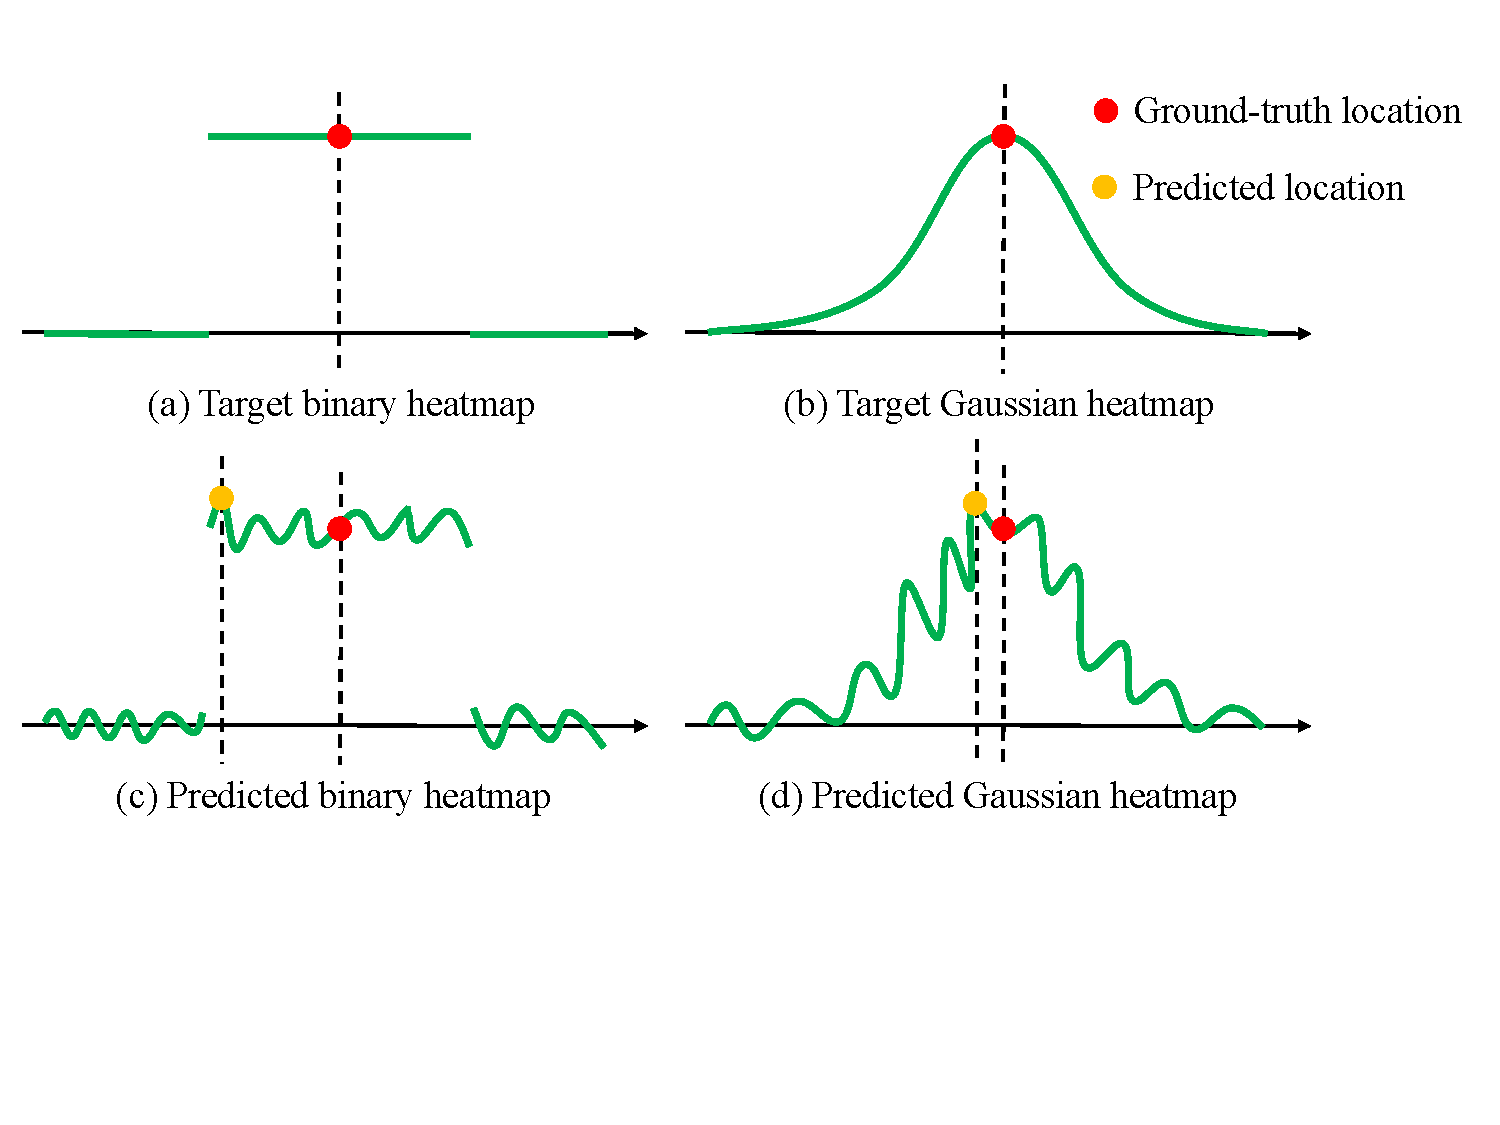
\includegraphics[width=15cm]{multiple_signal_detection/images/heatmap}}
	\caption{Schematics of target and predicted heatmaps. Drawn for a target rectangular distribution (\emph{a}, \emph{c}) and for a Gaussian distribution (\emph{b}, \emph{d}). Taken from \cite{wang2021lowresolutionhumanposeestimation}.}
	\label{fig:heatmap:rect_vs_gaussian}
\end{figure}

% delta peak not suited
% too sparse, and downsampling complications
% for this reason \cite{PhysRevD.100.063015} uses rect function
% following standard heatmap approach \cite{tompson2014jointtrainingconvolutionalnetwork} we use gaussian
% better time resolution see fig

In order to train models to predict such a heatmap $\hat{H}(t)$, it has to be considered what the ground-truth heatmap $H(t)$ should look like. It is natural to construct the ground truth as zeros everywhere except at the exact signal coalescence times, where a label of one is chosen. From a machine-learning perspective, however, this is problematic: For one, it makes the ground truth heavily imbalanced, which complicates training. Further, the models considered here downsample by a large factor of $256$, and the ground truth has to be downsampled accordingly. Sharp peaks can be lost in that process. (Alternatively, the ground truth could be downsampled with max pooling, but then some amount of time accuracy is lost.)

For these reasons, \cite{PhysRevD.100.063015} employs rectangles of width \SI{0.2}{\second}. However, following standard heatmap regression procedure \cite{tompson2014jointtrainingconvolutionalnetwork}, this work uses Gaussian distributions instead. This choice results in better peak extraction accuracy, as the peak of a Gaussian is clearly defined, which is not the case for a rectangular distribution (see Fig.~\ref{fig:heatmap:rect_vs_gaussian}). The ground truth is constructed from Gaussians with unit amplitude and standard deviation $\sigma=\SI{0.1}{\second}$. The distribution is centered on the corresponding signal coalescence time $t_{\text{coa}}$ and is truncated to a $3\,\sigma$ interval, 
\begin{equation}
	h(t) = \begin{cases}
		\exp{\frac{-(t-t_{\text{coa}})^2}{2\sigma^2}} & \text{if $|t-t_{\text{coa}}|\leq3\sigma$, } \\
		0 & \text{else.}
	\end{cases}
\end{equation}

\begin{figure}
	\centering
	\makebox[\textwidth]{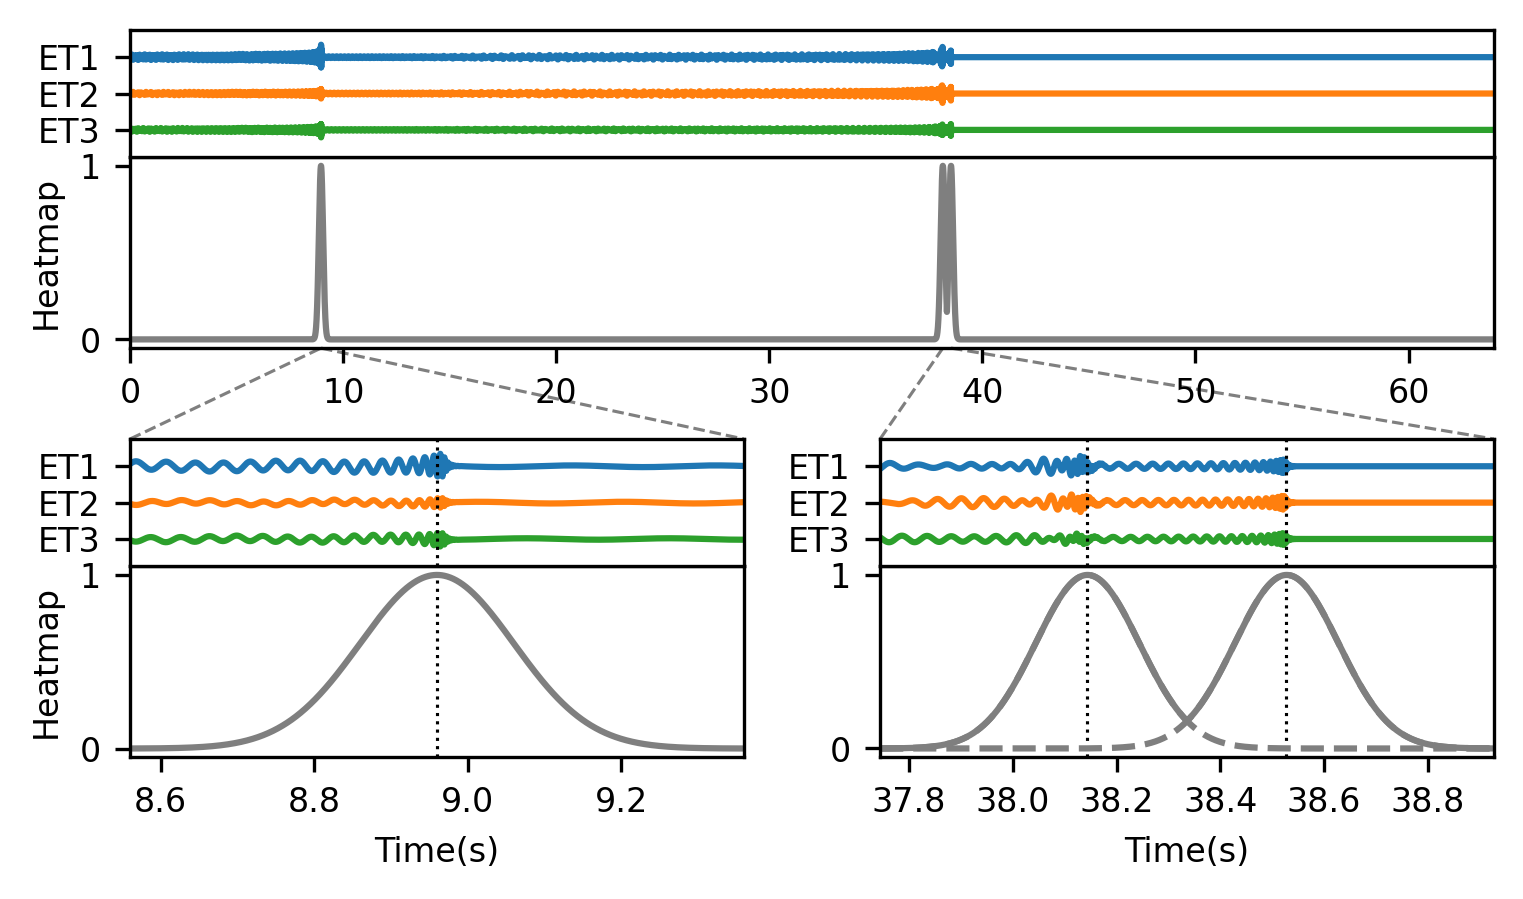
\includegraphics[width=15cm]{multiple_signal_detection/images/heatmap/sample}}
	\caption{Heatmap of a \SI{64}{\second} sample, constructed as the time-wise maximum of multiple Gaussians. Drawn on top of each plot are the individual detector \emph{signal} contributions. For better readability, only the signal and not the full signal + noise strain is shown.}
	\label{fig:heatmap:example_heatmaps}
\end{figure}

% overlapping signals?
% cannot be added up because heatmap has to be in [0,1]
% following \cite{law2019cornernetdetectingobjectspaired}, use max instead
% see fig

From multiple such distributions, a single heatmap could be naively constructed by summing them. However, this can result in heatmap values larger than one, which is impractical for training. Instead, this work follows \cite{law2019cornernetdetectingobjectspaired} and constructs the ground-truth heatmap using a time-wise max operation over all signal distributions, 
\begin{equation}
	H(t) = \max(h_1(t), h_2(t), \dots).
\end{equation}
If a sample contains no signals, $H(t)=0$. See an example heatmap in Fig.~\ref{fig:heatmap:example_heatmaps}.

% postprocessing
% get all peaks with min delta of 1sigma
% score is the peak value
% around each peak estimate sub pixel position according to \cite{bulat2021subpixelheatmapregressionfacial}
% use region of 2 sigma
% softmax
% time is weighted mean

GW candidates are extracted from the predicted heatmap $\hat{H}(t)$ via a peak finding algorithm. All peaks, regardless of height, are extracted. Thresholds are applied later when computing operating points. A minimum distance of \SI{0.1}{\second} is enforced between peaks. For this, methods implemented by SciPy~\cite{2020SciPy-NMeth} are relied upon. 

The extracted peak positions are denoted $x_i$. The GW candidate scores are the peak heatmap values, $\hat{c}_i = \hat{H}(x_i)$. For the corresponding time prediction $\hat{t}_i$, sub-pixel accuracy is achieved with a \emph{soft argmax} operation \cite{bulat2021subpixelheatmapregressionfacial}, which is applied locally around peaks. 

To this end, for each peak $x_i$, the predicted heatmap values outside a $1\,\sigma$ radius are masked. This can be written as,
\begin{equation}
	w_i(t) = \begin{cases} 
		\hat{H}(t) & |t-x_i| < \sigma \\
		-\infty & \text{else.}
	\end{cases}
\end{equation} 
Setting masked values to $-\infty$ will be justified later on. Then, the time-prediction $\hat{t}_i$ is estimated as the soft argmax of $w_i$, 
\begin{equation}
	\hat{t}_i = \sum_t \softmax{(w_i)}(t)\,t.
\end{equation}
% TODO: ugly sentence
The softmax operation, 
\begin{equation}
\softmax{\vec{x}} = \frac{1}{\sum_i \e^{x_i}} \begin{pmatrix}
	\e^{x_0} & \e^{x_1} & \dots & \e^{x_{N-1}}
\end{pmatrix}^\intercal,
\end{equation} 
ensures that the values of $\softmax{(w_i)}(t)$ sum to one and returns zeros outside the considered $1\,\sigma$-radius, where $w_i(t) = -\infty$.

\section{CNN and Transformer Models}

\begin{figure}
	\centering
	\makebox[\textwidth]{
		\includegraphics[width=7.5cm]{multiple_signal_detection/images/heatmap_CNN}
		\hspace{0cm}
		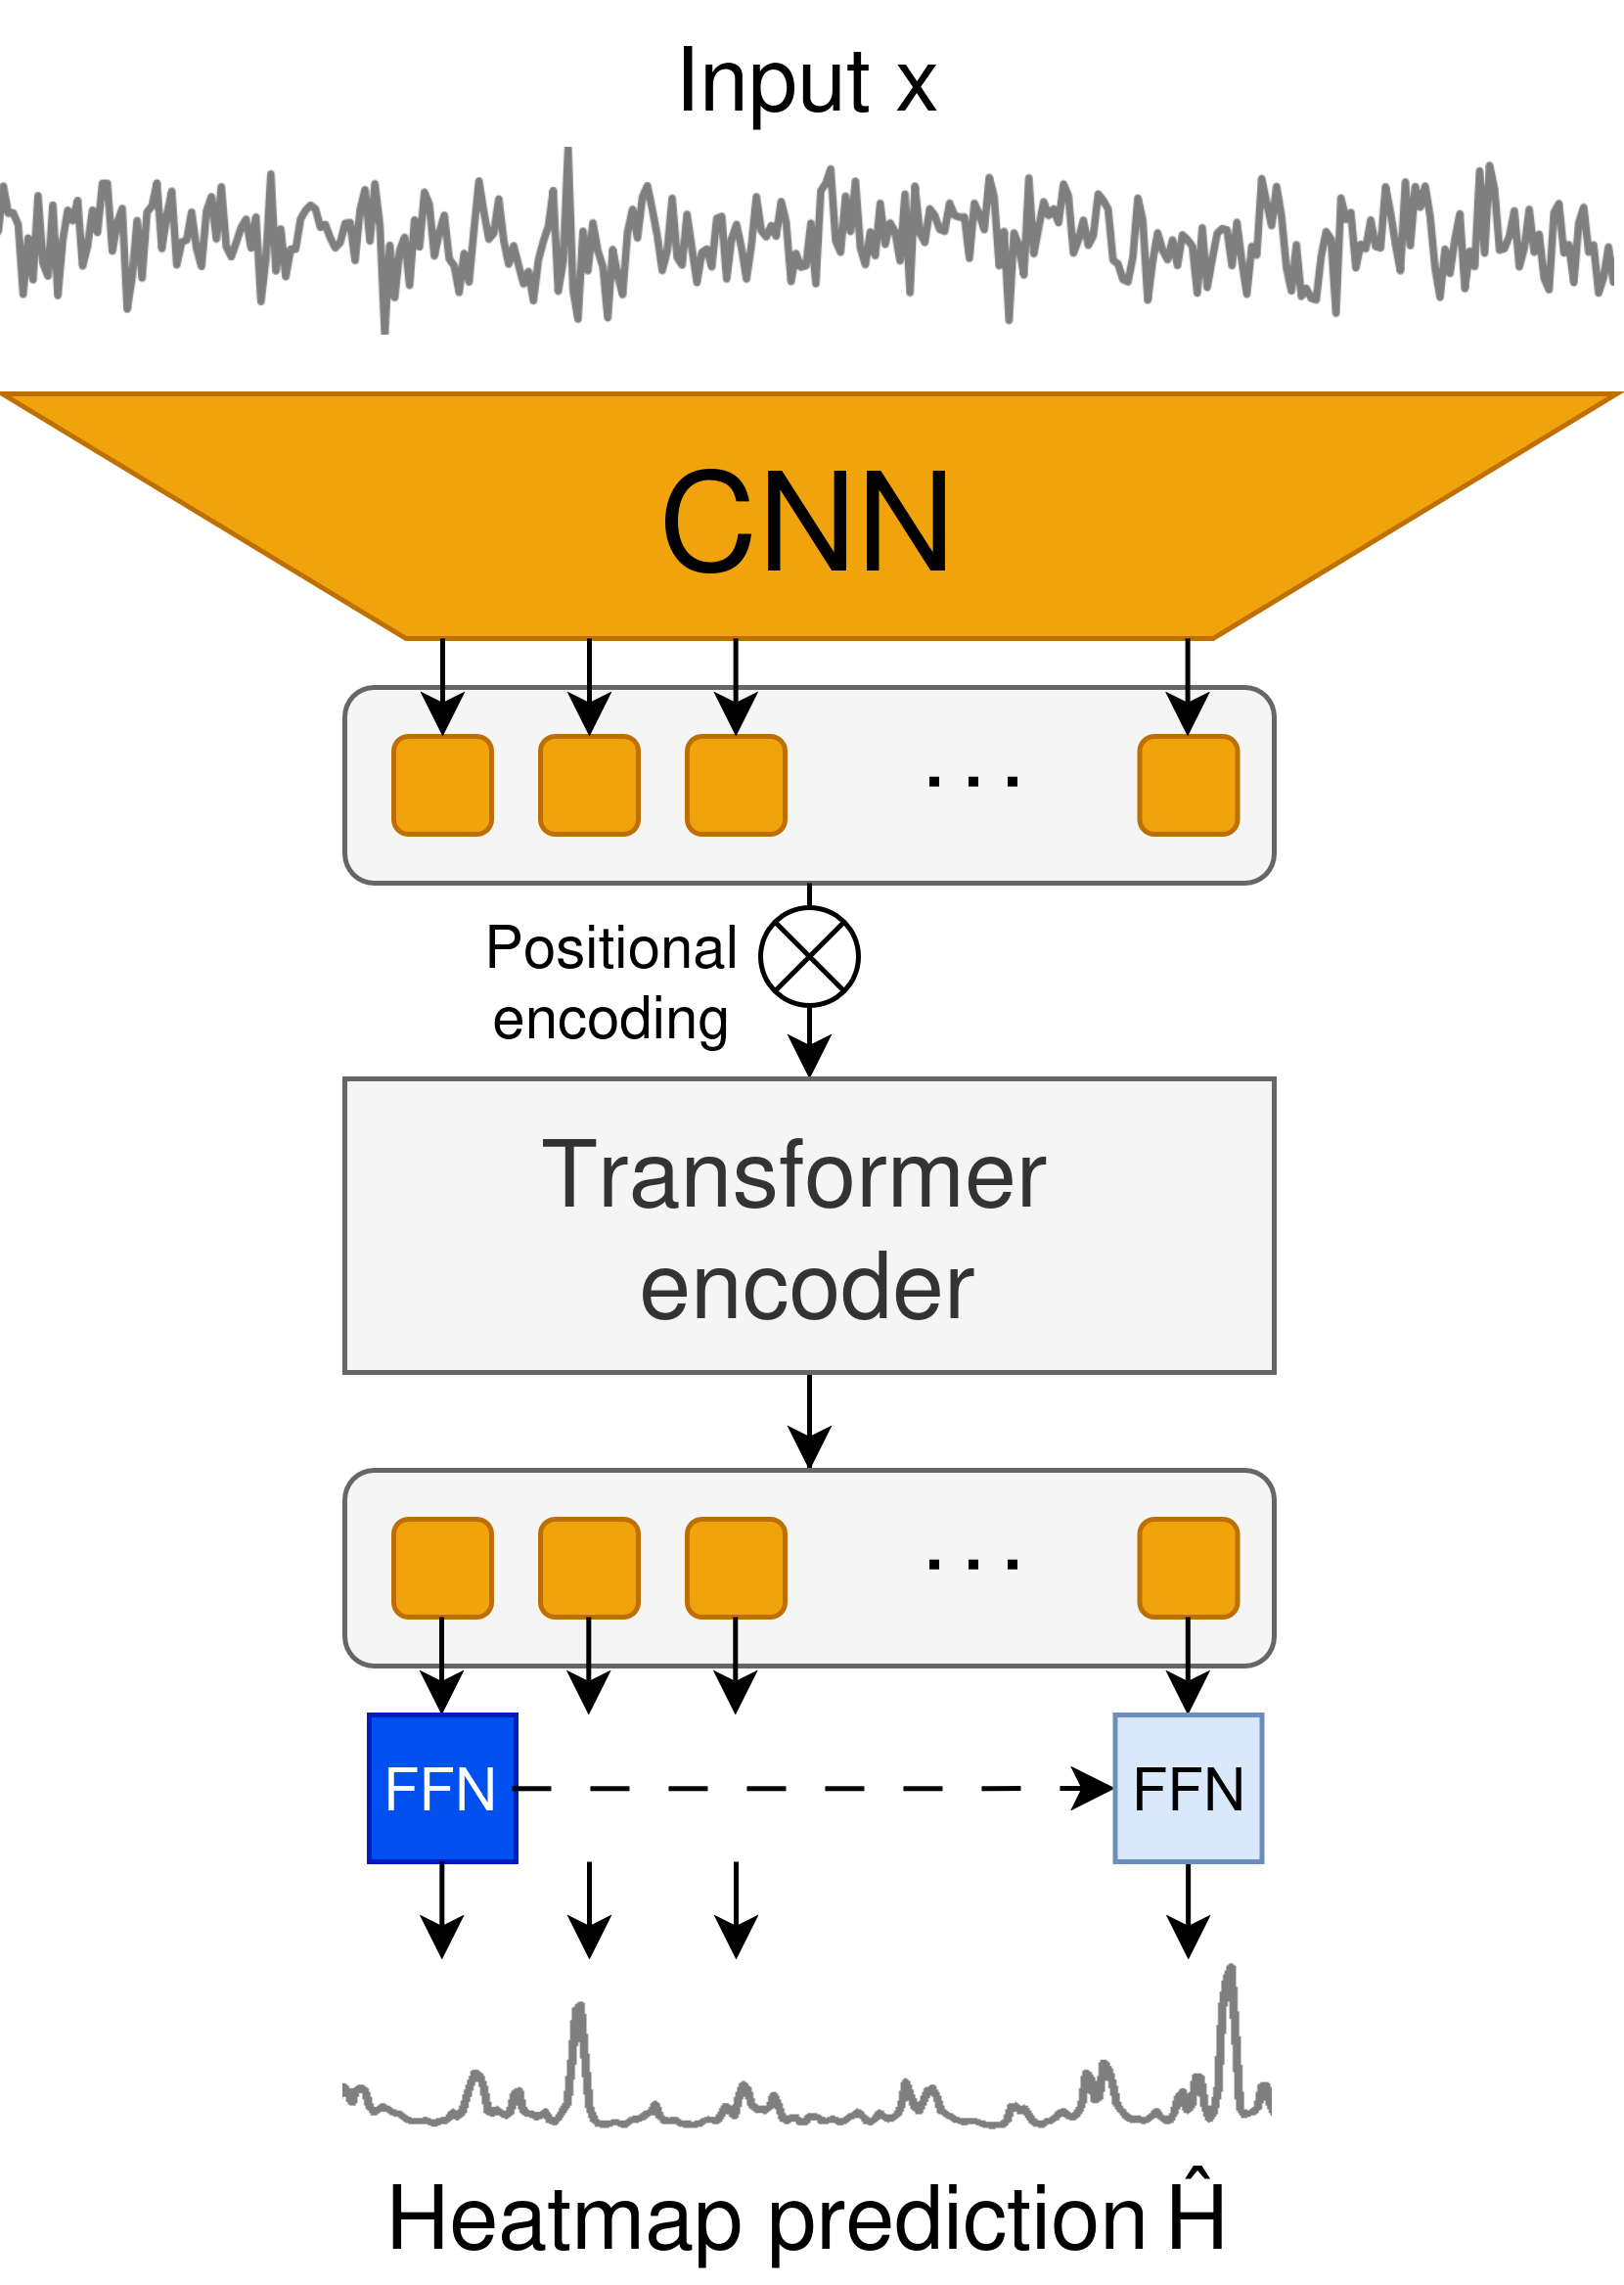
\includegraphics[width=7.5cm]{multiple_signal_detection/images/heatmap_transformer}
	}
	\caption{Schematics of the CNN (\emph{left}) and the transformer encoder (\emph{right}) heatmap regressor models.}
	\label{fig:heatmap:models}
\end{figure}

% two models one cnn and one transformer encoder model with cnn tokenizer
% adjust previous models
% CNN no avg pool and cls head, but sliding cls head
% 700k params
% transformer no cls token, slide cls head over all output tokens
% sinsuoidal pos encondings, embed dim of 64, 8 heads, 6 layers
% 2.2M params

Motivated by the results in \cite{Papalini_2025}, this chapter compares one CNN-based and one transformer-based heatmap regressor. For this, the models implemented in Ch.~\ref{sec:long_duration} are repurposed. The CNN model is the same ResNet model that was presented in the previous chapter. Only the average pooling over the time dimension is discarded. The classification head is then applied over all downsampled time steps to produce a heatmap of length $512$. The classification head is a FFN that takes a vector with $256$ features and returns one number, 
%\begin{equation}
%	\label{eq:heatmap:classification_head}
%	z = \text{Dropout}(\text{Linear}_{1024\rightarrow1}(\text{ReLU}(\text{Dropout}(\text{Linear}_{256\rightarrow1024}(\text{BatchNorm}(x))))))
%\end{equation}
\begin{equation}
\begin{aligned}
	\label{eq:heatmap:classification_head}
	n &= \mathrm{BatchNorm}(x),\\
	h &= \mathrm{Dropout}(\mathrm{ReLU}(\mathrm{Linear}_{256\rightarrow1024}(n))),\\
	z &= \mathrm{Dropout}(\mathrm{Linear}_{1024\rightarrow1}(h)),
\end{aligned}
\end{equation}
with a dropout probability of \SI{10}{\percent}. The output is later passed through a sigmoid activation to yield heatmap values in $[0,1]$. The model has a total of \SI{700}{\kilo\nothing} parameters. Apart from the exact implementation of the CNN and classification head, this architecture is the same as \cite{PhysRevD.100.063015}.

Similar to the ViT, the transformer model considered here consists of a transformer encoder only. The model uses the same ResNet for tokenization, again, resulting in $512$ tokens with embedding dimension $d_\text{embed}=64$. Instead of appending a single classification token, \emph{all} encoder output tokens are fed through a classification head. This is an FFN similar to Eq.~\ref{eq:heatmap:classification_head} with an input size of $64$ instead, and yields a heatmap of length $512$. The model employs sinusoidal positional encodings, and the encoder consists of six layers and eight heads. The transformer FFNs have $d_\text{ff}=1024$. A dropout probability of \SI{10}{\percent} is used throughout. The total number of trainable parameters is \SI{2.2}{\mega\nothing}. See schematics of both the CNN and transformer encoder models in Fig.~\ref{fig:heatmap:models}. 

% training is complicated by positive label sparsity
% use time-wise bce loss, weighting positive label by a large factor of 0.98
% (often in heatmap regression, more complicated losses are used because element-wise losses cannot appropriately measure the difference between distributions) 

The model weights are optimized by minimization of the time-wise BCE loss of the ground truth and predicted heatmap $H(t)$ and $\hat{H}(t)$. For ground-truth labels continuous in $[0,1]$, this is defined as,
\begin{equation}
	\pazocal{L}_\text{BCE}(H(t), \hat{H}(t)) = -(\alpha H(t) \ln{\hat{H}(t)} + (1 - \alpha) (1-H(t)) \ln{(1-\hat{H}(t))}).
\end{equation}
Because of label sparsity, the loss term corresponding to positive labels is up-weighted by a factor $\alpha$ and the other term down-weighted by $(1-\alpha)$. For this, a relatively high positive-label weight of $\alpha = 0.98$ is chosen empirically. In practice, this loss is calculated from the pre-sigmoid logits.

% AdamW lw 1e-4 weightdecay 1e-4
% CNN reduce on plateau (factor: 0.1, patience: 15, threhsold: 0.01)
% cosine annealing with warmup of 5000 steps

Models are trained for a maximum of $100$ epochs using the AdamW optimizer with a learning rate of \SI{E-4}{\nothing} and a weight decay of \SI{E-4}{\nothing}. The batch size is $64$. For the CNN model, the learning rate is reduced by a factor $0.1$ if the validation loss does not decrease by at least $0.01$ over $15$ epochs. The encoder model is trained with a cosine-annealing schedule with a warmup of $5000$ steps. 

\begin{figure}
	\centering
	\makebox[\textwidth][c]{%
		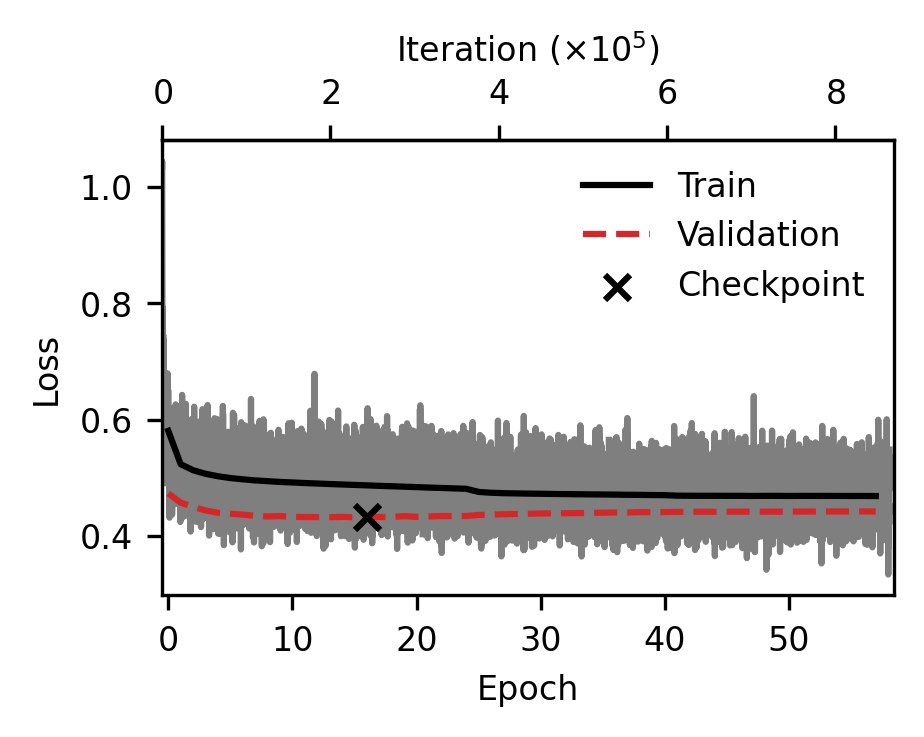
\includegraphics[width=8cm]{multiple_signal_detection/plots/learning_curves/cnn_loss}%
		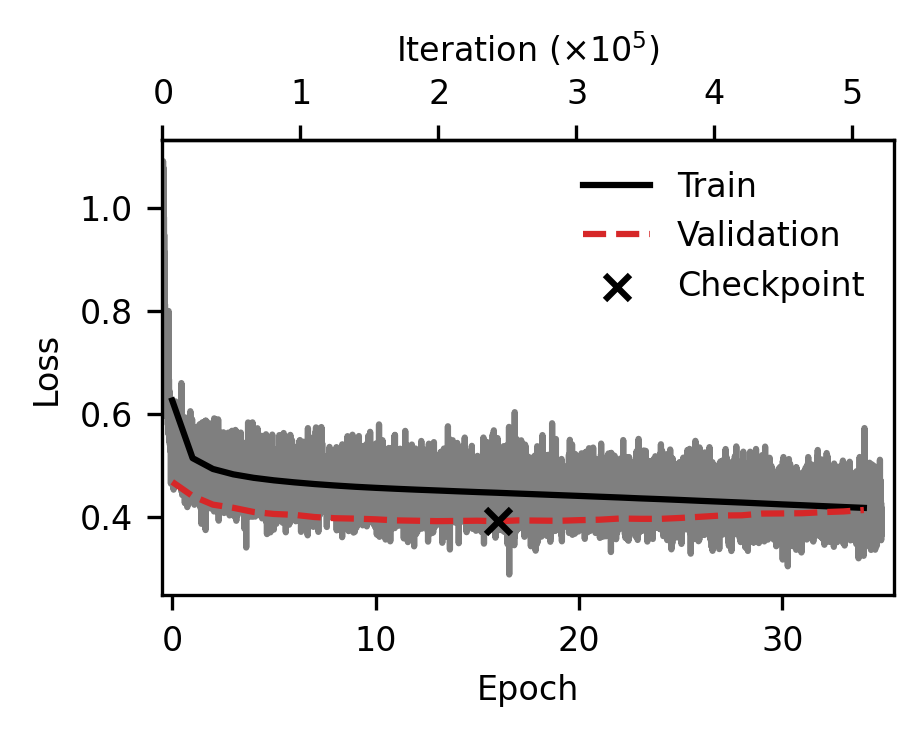
\includegraphics[width=8cm]{multiple_signal_detection/plots/learning_curves/encoder_loss}
	}
	\caption{Learning curves of the CNN (\emph{left}) and the encoder model (\emph{right}). The training loss is plotted for each step (\emph{grey}) and as averaged over all steps in one epoch (\emph{black}). The validation loss is plotted in red and a marker signifies its minimum.}
	\label{fig:heatmap:learning_curves}
\end{figure}

% see learning curve in fig
% similar to the vit learning curves, the plot shows lower validation loss because of final dropout layer

See both learning curves in Fig.~\ref{fig:heatmap:learning_curves}. Both models start to overfit after $16$ epochs. Similar to the ViT learning curves, the plot shows a lower validation loss in the early epochs because of the classification head's final dropout layer.

\section{Performance Comparison}

\begin{figure}
	\centering
	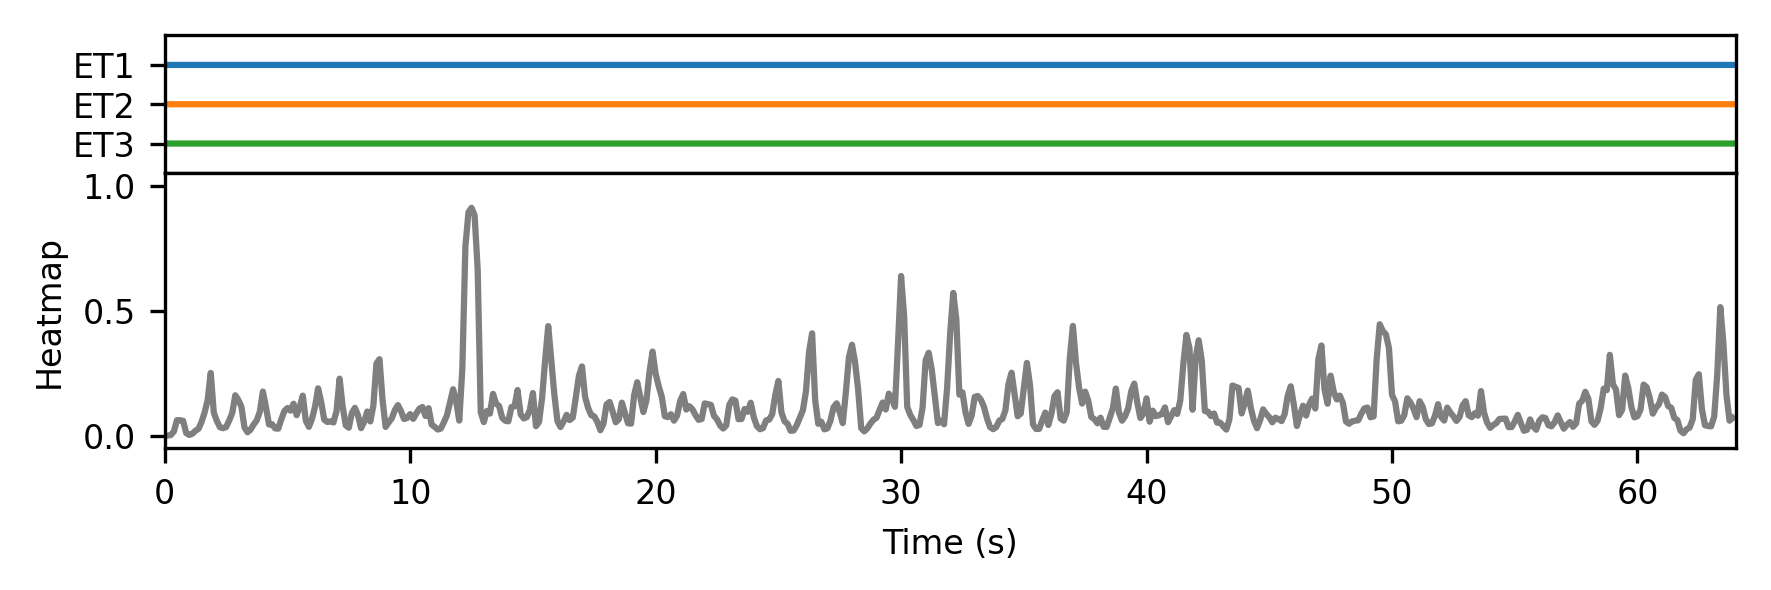
\includegraphics[
	width=15cm,
	trim=0 1cm 0 0,
	clip
	]{multiple_signal_detection/plots/out/300/encoder/11}
	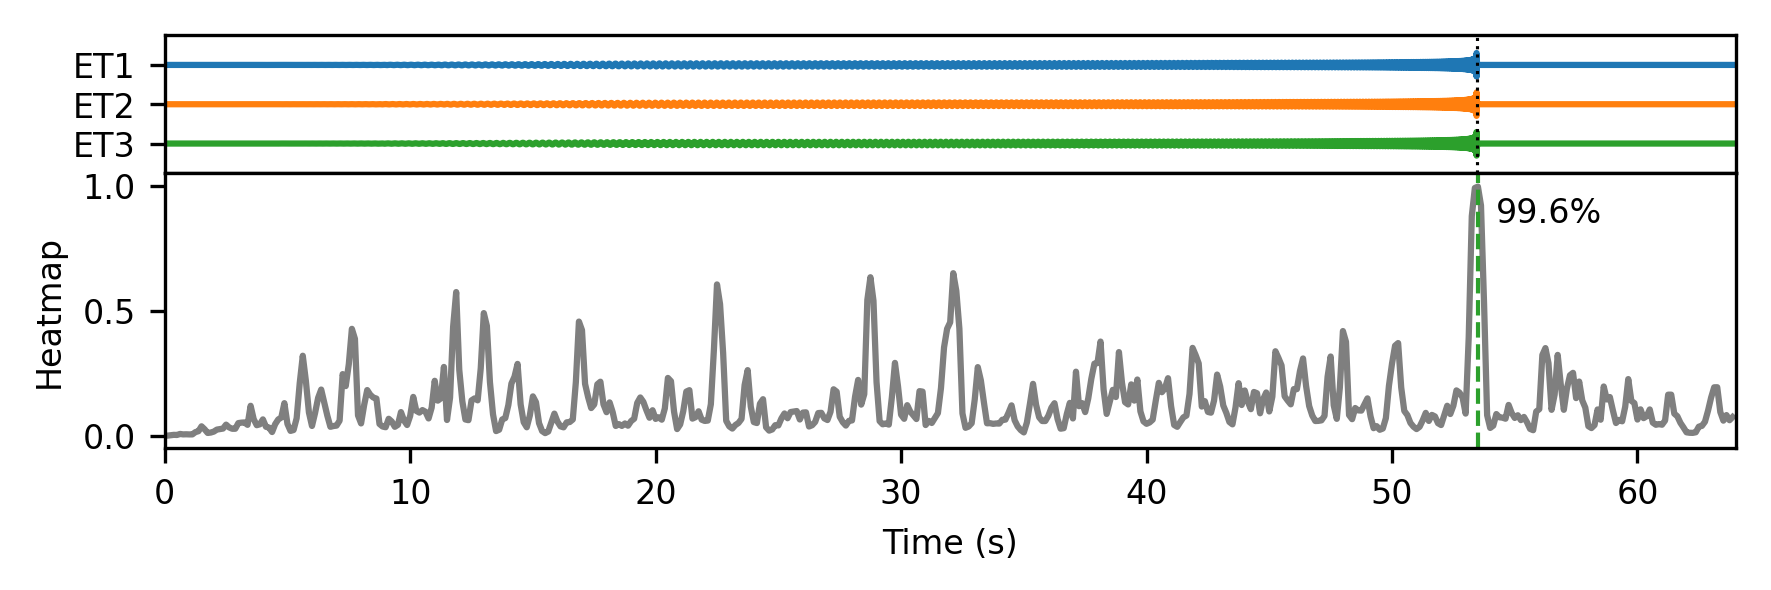
\includegraphics[
	width=15cm,
	trim=0 1cm 0 0,
	clip
	]{multiple_signal_detection/plots/out/300/encoder/1}
	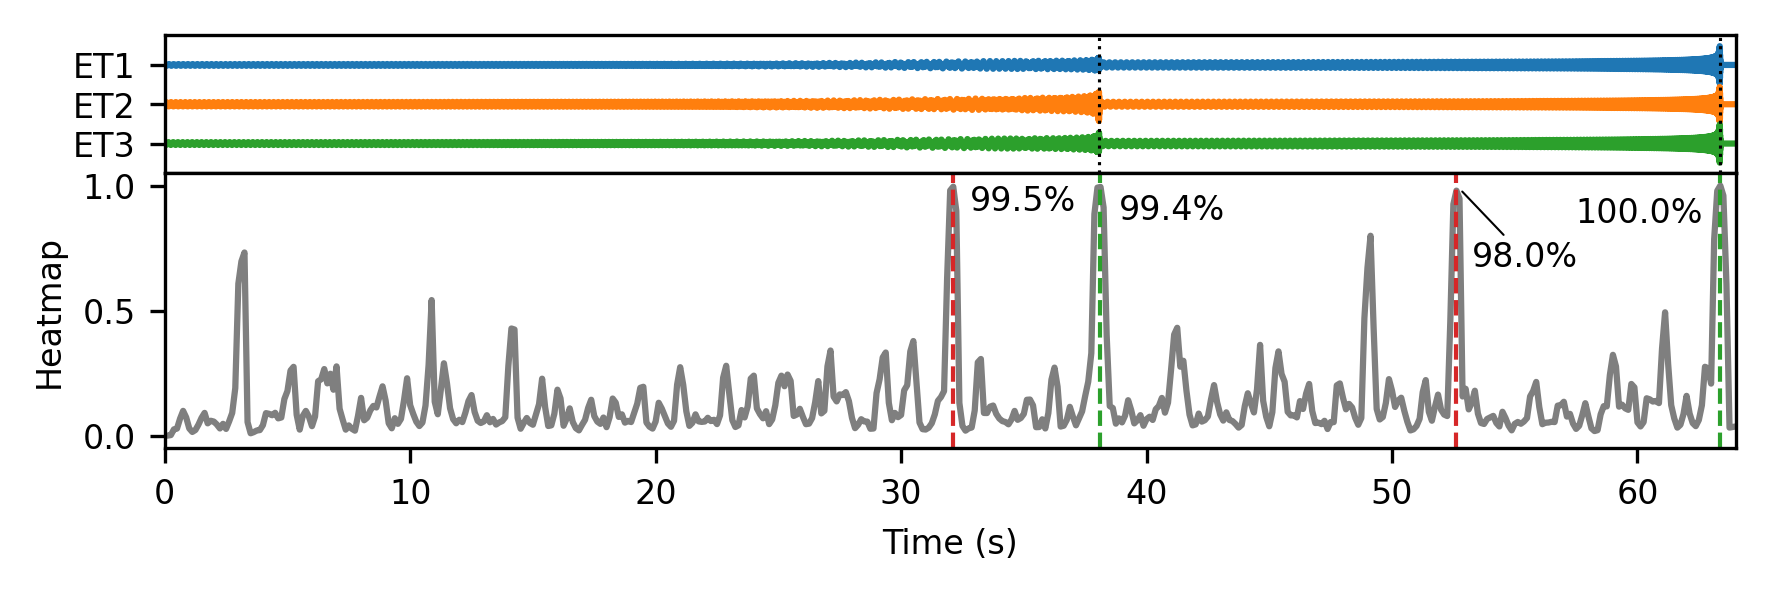
\includegraphics[
	width=15cm,
	trim=0 1cm 0 0,
	clip
	]{multiple_signal_detection/plots/out/300/encoder/3}
	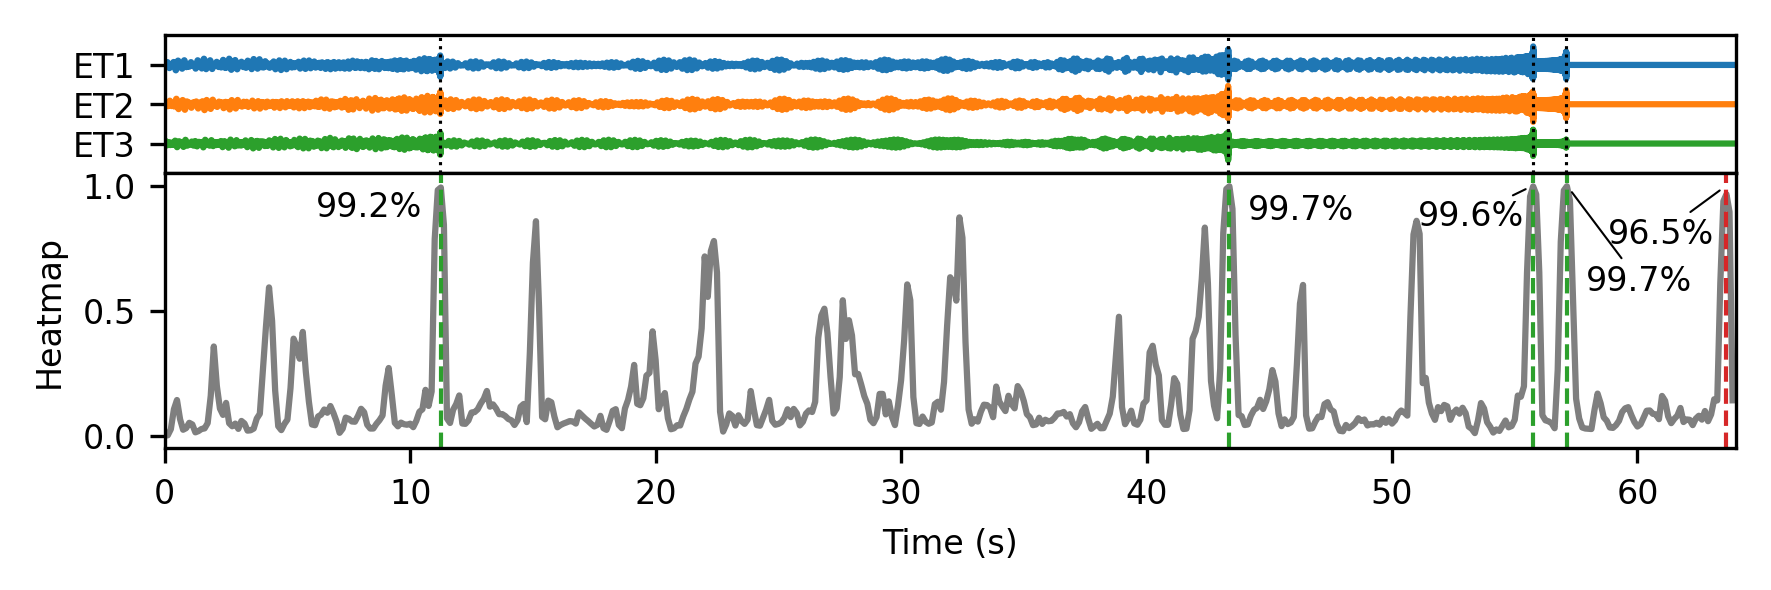
\includegraphics[
	width=15cm,
	trim=0 1cm 0 0,
	clip
	]{multiple_signal_detection/plots/out/300/encoder/0}
	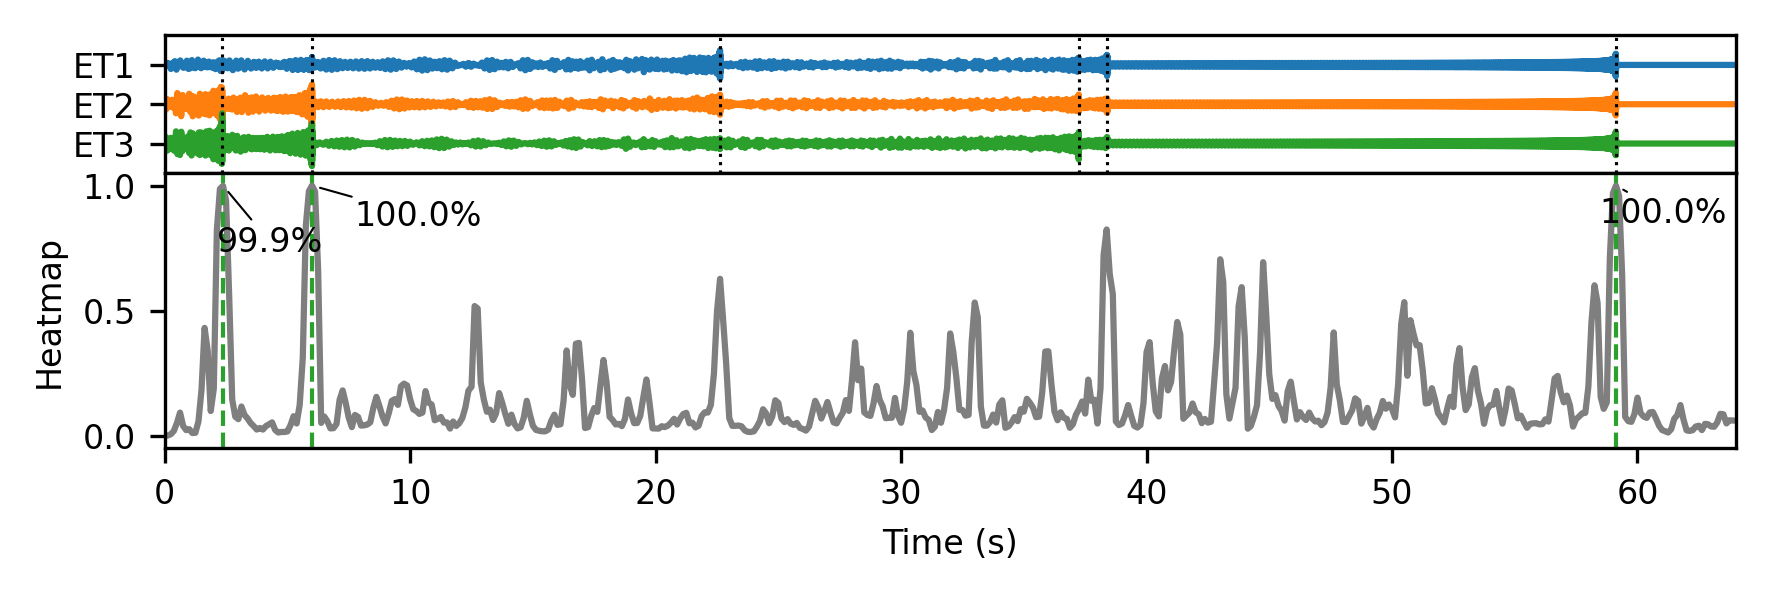
\includegraphics[
	width=15cm,
	]{multiple_signal_detection/plots/out/300/encoder/8}
	\caption{Predicted heatmaps for five samples produced by the encoder model. Peaks above a threshold of \SI{96}{\percent} are GW candidates. For each candidate, the class score is indicated and the time prediction is shown as a vertical line. This line is colored green for TPs and red for FPs.}
	\label{fig:heatmap:encoder_out}
\end{figure}

% get a sense of whats going on see fig
% network is quite trigger happy -> high positive weight
% still when using a high threshold of 96.0%, most signals can be retrieved while not producing too many FPs (the choice of this threshold will justified soon)
% The time resolution seems too be sufficient. In these 5 example samples, no prediction is labeled FP because it differs more than 0.1s from the correspondiing merger

Before evaluating the models quantitatively, it is useful to inspect individual predicted heatmaps. Fig.~\ref{fig:heatmap:encoder_out} shows the transformer encoder model's output for five test samples. It can be seen that the model is quite trigger-happy, producing $\approx100$ peaks per sample. This behavior is expected to some extent, as the models were trained with a high positive weight. Still, by employing a relatively high score threshold of \SI{96}{\percent}, most signals can be retrieved without producing too many FPs. (The exact value of that threshold depends on the desired FAR. This will be covered later.) Further, it appears that the predicted time resolution is sufficient for the chosen matching criterion: In the examples shown, no prediction is labeled FP because the time prediction differs by more than \SI{0.1}{\second} from the ground-truth signal coalescence time.

\begin{figure}
	\centering
	\makebox[\textwidth]{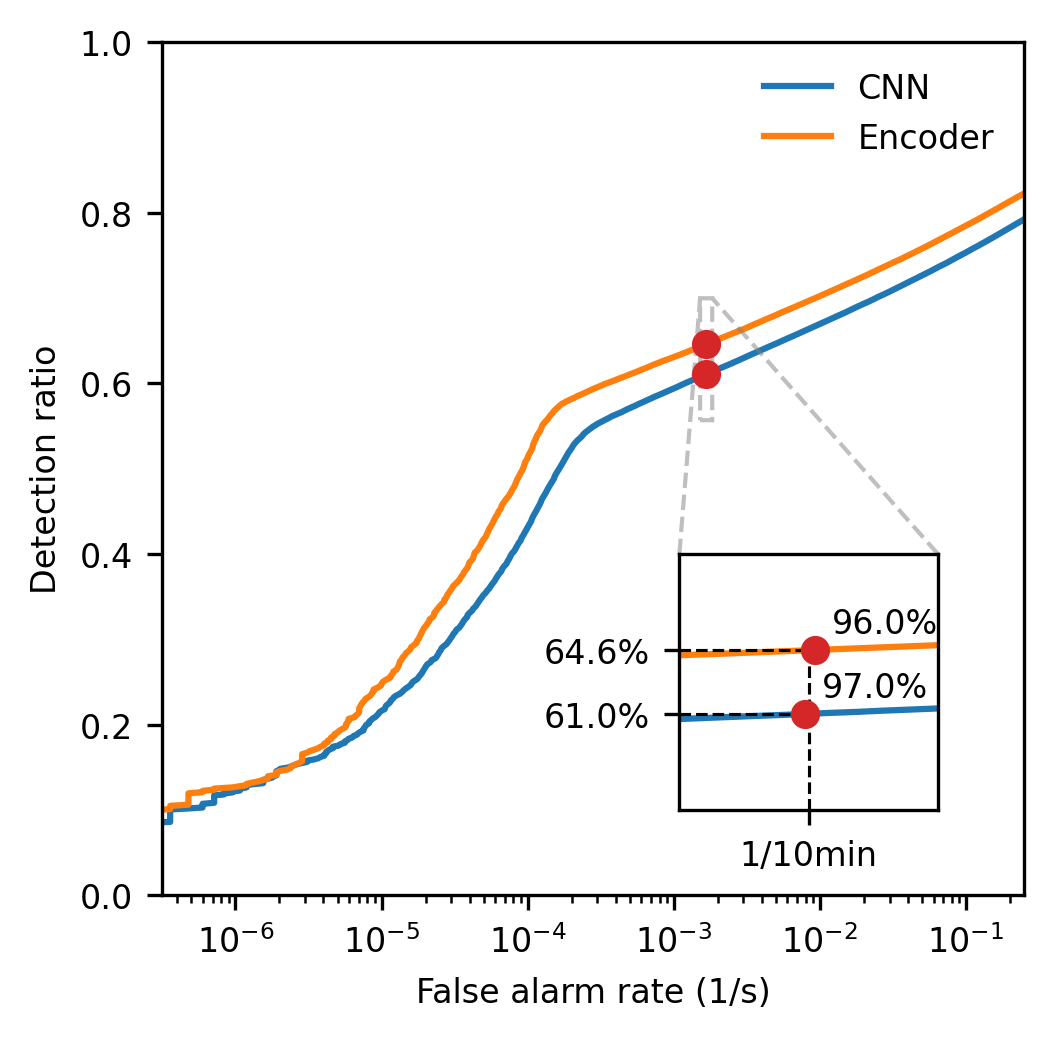
\includegraphics[width=9cm]{multiple_signal_detection/plots/cnn_encoder_far}}
	\caption{Detection ratio as a function of FAR for the CNN (\emph{blue}) and transformer encoder (\emph{orange}) models. Computed over  \SI{131}{\kilo\nothing} test samples containing \SI{393}{\kilo\nothing} signals. The upper FAR limit corresponds to $16$ FPs per sample, and the lower limit is $1/\SI{}{\month}$. Markers indicate the fixed operating points, where $\text{FAR}=1/\SI{10}{min}$. For each marker, the corresponding threshold is written out. Uncertainties are too small to be visualized.}
	\label{fig:heatmap:encoder_far}
\end{figure}

% more robust way of estimating performance, also too compare cnn and encoder model
% plot operating characteristic of FAR, detection ratio for different thresholds
% see the results in fig
% models reach quite low FAR of 1/month while retaining some amount of signals (10% to 20%)

A robust performance test is obtained by varying the score threshold and computing the detection ratio and FAR over the whole test dataset. The detection ratio is computed over \SI{393}{\kilo\nothing} signals. This gives a maximum uncertainty of \SI{0.08}{\percent}, assuming a binomial distribution\footnote{Strictly speaking, this assumption is wrong, as trials are not independent when dealing with overlapping signals. In particular, it will become clear that the detection ratio decreases for closely separated signals. Still, the results will show that this effect is only relevant for signals with separations $\leq\SI{0.6}{\second}$, which does not amount to a large number of signals. Thus, the binomial uncertainty still serves as a useful estimate.}. The operating characteristics for the CNN and transformer encoder models are shown in Fig.~\ref{fig:heatmap:encoder_far}. Both models reach low FARs while retaining a non-zero fraction of signals. At a FAR of $1/\SI{}{\month}$, the detection ratio is $\approx\SI{10}{\percent}$. The encoder model performs better over the whole FAR range shown in Fig.~\ref{fig:heatmap:encoder_far}. 

To evaluate and compare the models' performance, fixed operating points have to be chosen. While low-latency searches usually aim for FARs of $1/\SI{}{\month}$, the models here do not perform particularly well in this regime. For the purposes of this study, a FAR of $1/\SI{10}{\minute}$ is employed instead, which corresponds to approximately one FP every ten samples. At the corresponding operating points, the models achieve good performance, while not producing too many FPs. For this, the threshold is set to \SI{97.0}{\percent} for the CNN and to \SI{96.0}{\percent} for the encoder model. The CNN reaches a detection ratio of \SI{61.04(8)}{\percent}, while the transformer encoder reaches \SI{64.61(8)}{\percent}. 

At this point, it is natural to ask how this performance compares to matched filtering. A direct comparison is not attempted here because implementing a full matched-filtering search goes beyond the scope of this thesis. Moreover, a quantitative comparison to existing research is complicated by the fact that the datasets used can differ significantly:
\begin{itemize}
	\item For one, studies often employ the lower event-rates of second-generation detectors. It has been shown that for strongly time-overlapping signals, the performance of matched filtering decreases \cite{Relton_2022}. Because of ET's higher event-rate, these overlaps occur frequently in this work's simulations.
	\item Datasets differ in the chosen signal parameters. This matters especially for the component masses, as Ch.~\ref{sec:long_duration} showed that model performance depends strongly on these.
	\item Most importantly, datasets differ in the considered signal SNR. In this work, the SNR is sampled uniformly in $[5,15]$. Studies often sample the distance from a second order power law instead, resulting in a non-uniform SNR distribution. For example, \cite{Relton_2022} reports SNRs up to $50$, which is much louder than this work's test dataset.
\end{itemize}
For these reasons, comparisons to matched filtering will be qualitative in the following. As a rough estimate, offline searches~\cite{Nitz_2017, Relton_2022} reach close to perfect detection ratios for signal SNRs larger than $10$ to $15$ and at FARs $<1/\SI{}{\year}$. For the SNR range considered here, this very loosely translates to a detection ratio of \SI{50}{\percent}. Online searches~\cite{Nitz_2018} reach comparable performance at a FAR of $1/\SI{}{\month}$. Compare this to the detection ratio of $\approx\SI{10}{\percent}$ at a FAR of $1/\SI{}{\month}$, reached by the models here.

\begin{figure}
	\centering
	\makebox[\textwidth]{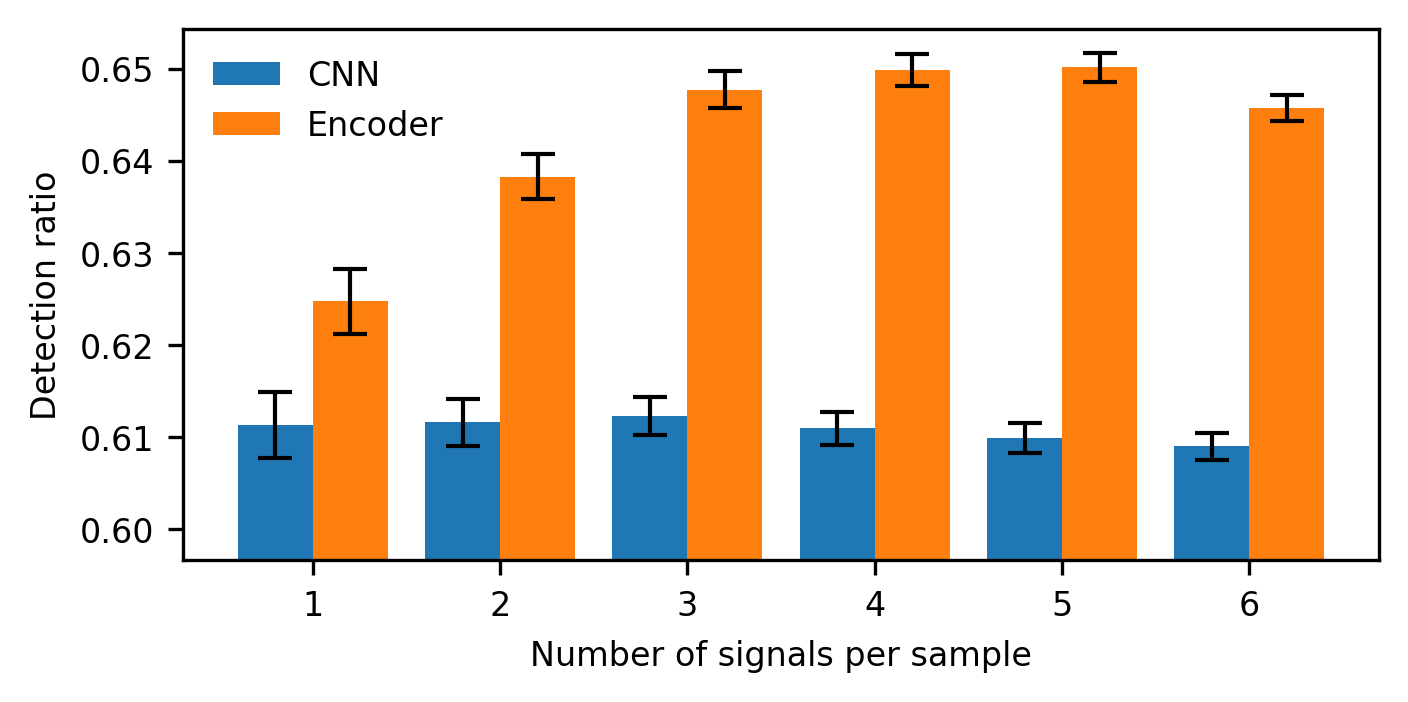
\includegraphics[width=12cm]{multiple_signal_detection/plots/cnn_encoder_mergers}}
	\caption{Detection ratio as a function of $n$, the number of signals per sample, for the CNN (\emph{blue}) and the encoder model (\emph{orange}). Computed over $\SI{19}{\kilo\nothing}$ samples each. The number of signals per sample can be taken as a measure of signal overlap.}
	\label{fig:heatmap:num_mergers}
\end{figure}

% \cite{Papalini_2025} report transformers being good for overlapping signals
% check detection ratio as a function of signals per sample
% see plot
% similar performance if one signals per sample
% CNN decreases for more signals
% interestingly, encoder slightly increases in performance

The results so far show that the transformer model outperforms the conventional CNN approach. Motivated by \cite{Papalini_2025}, it is tempting to attribute this result to the increased signal overlap in the data. This can be tested by examining the detection ratio (at the fixed operating points defined earlier) as a function of the number of signals per sample $n$. Since the sample size is \SI{64}{\second}, multiple signals, $n>1$, will almost always overlap. For this, the test dataset is binned with $n\in[1,6]$ resulting in six subsets of \SI{19}{\kilo\nothing} samples each. These contain \SI{19}{\kilo\nothing}, \SI{37}{\kilo\nothing}, \dots signals, respectively. For each subset, the detection ratio is computed separately, assuming a binomial distribution for the uncertainty. See the results in Fig.~\ref{fig:heatmap:num_mergers}.

The plot shows that both models perform similarly if there is only one signal per sample $n=1$. For increasing $n$, the CNN model stays mostly constant in performance as the detection ratio decreases by $\SI{0.3(3)}{\percent}$ only.
Interestingly, the transformer encoder's detection ratio \emph{increases} by $\SI{2.5(4)}{\percent}$ instead. Thus, the performance difference stems mainly from those samples with multiple overlapping signals: not because increased overlap degrades the CNN performance, but because the encoder improves with more signals per sample.

This difference is likely explained by the models' \emph{receptive fields}. For the CNN, at each time step, the classification head can only attend to $\approx\SI{1}{\second}$ of data. In contrast, in the  transformer encoder model, the classifier can attend to the whole input time series through the \emph{attention mechanism}.
As the CNN does not degrade in performance, it can be argued that its small local receptive field of $\approx\SI{1}{\second}$ is sufficient for capturing signal overlap. This is consistent with \cite{Relton_2022}, where overlap only becomes problematic for signals with coalescence times separated by $<\SI{1}{\second}$. The effect of signal separation on model performance is studied more closely in the following sub-chapter.

\begin{figure}
	\centering
	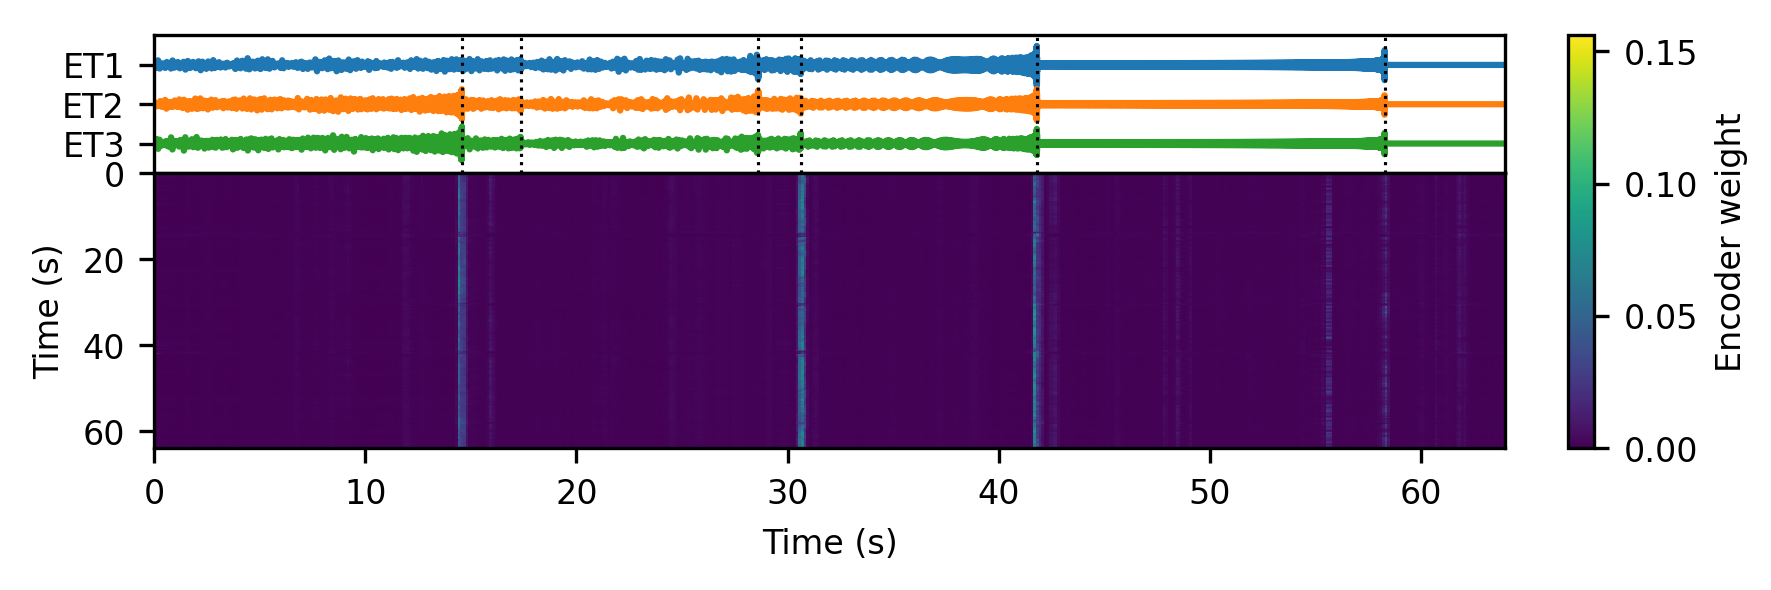
\includegraphics[
	width=15cm,
	trim=0 1cm 0 0,
	clip
	]{multiple_signal_detection/plots/weights/encoder/11}
	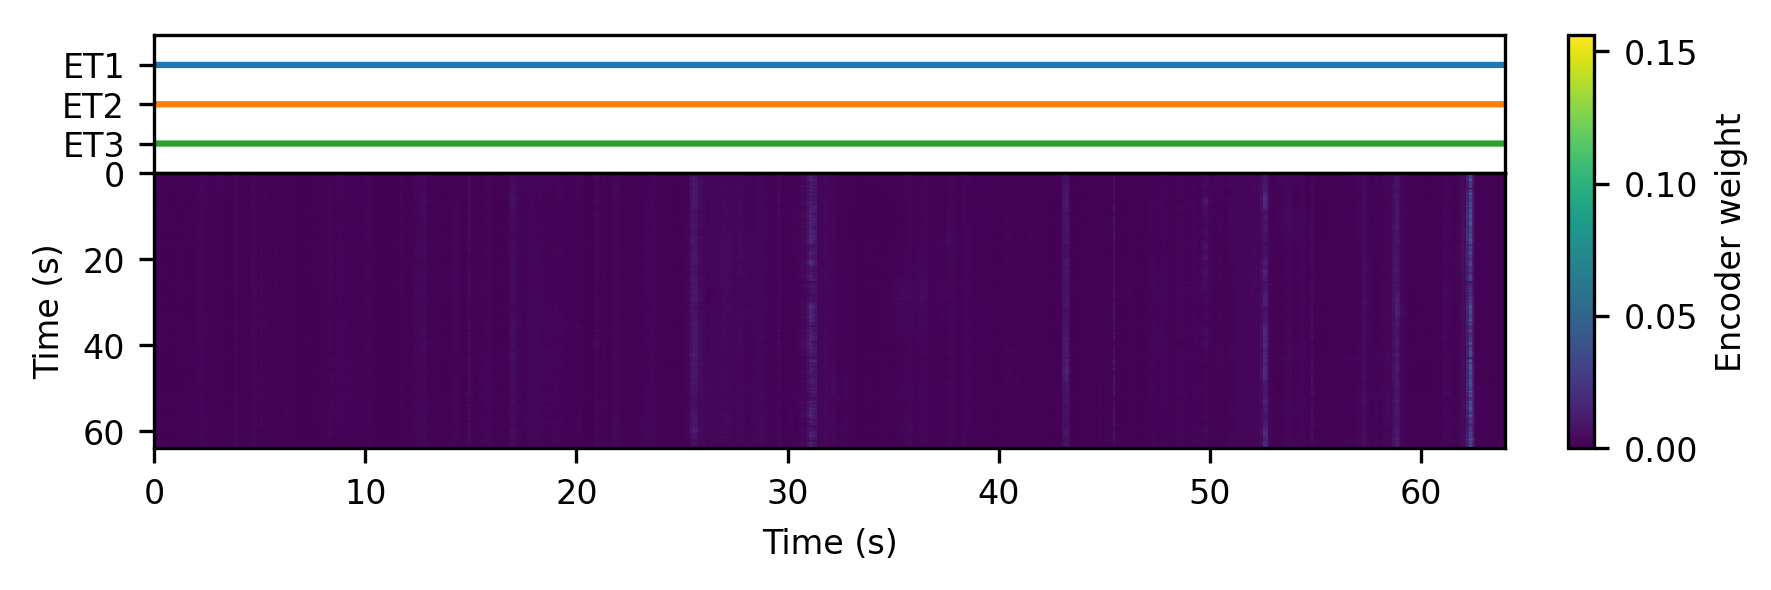
\includegraphics[
	width=15cm,
	trim=0 1cm 0 0,
	clip
	]{multiple_signal_detection/plots/weights/encoder/1}
	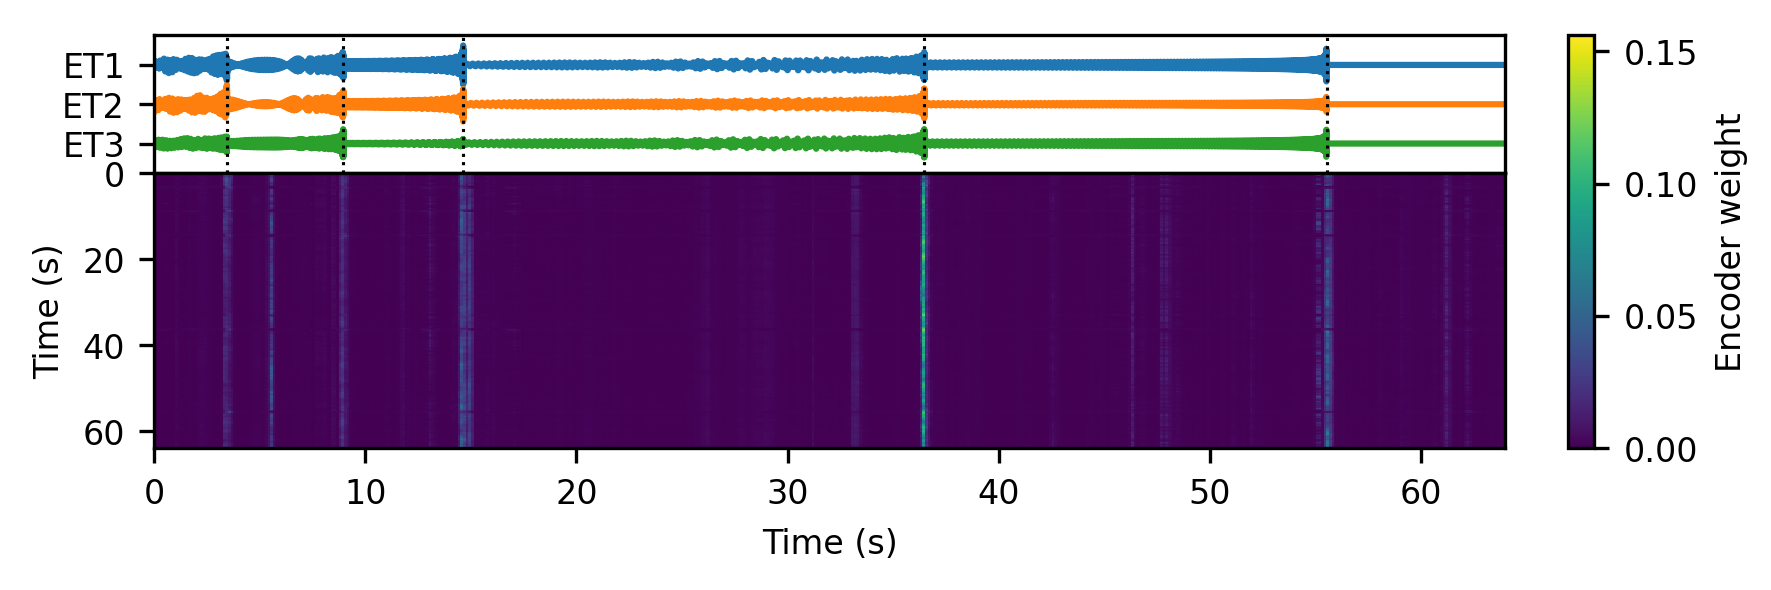
\includegraphics[
	width=15cm,
	trim=0 1cm 0 0,
	clip
	]{multiple_signal_detection/plots/weights/encoder/3}
	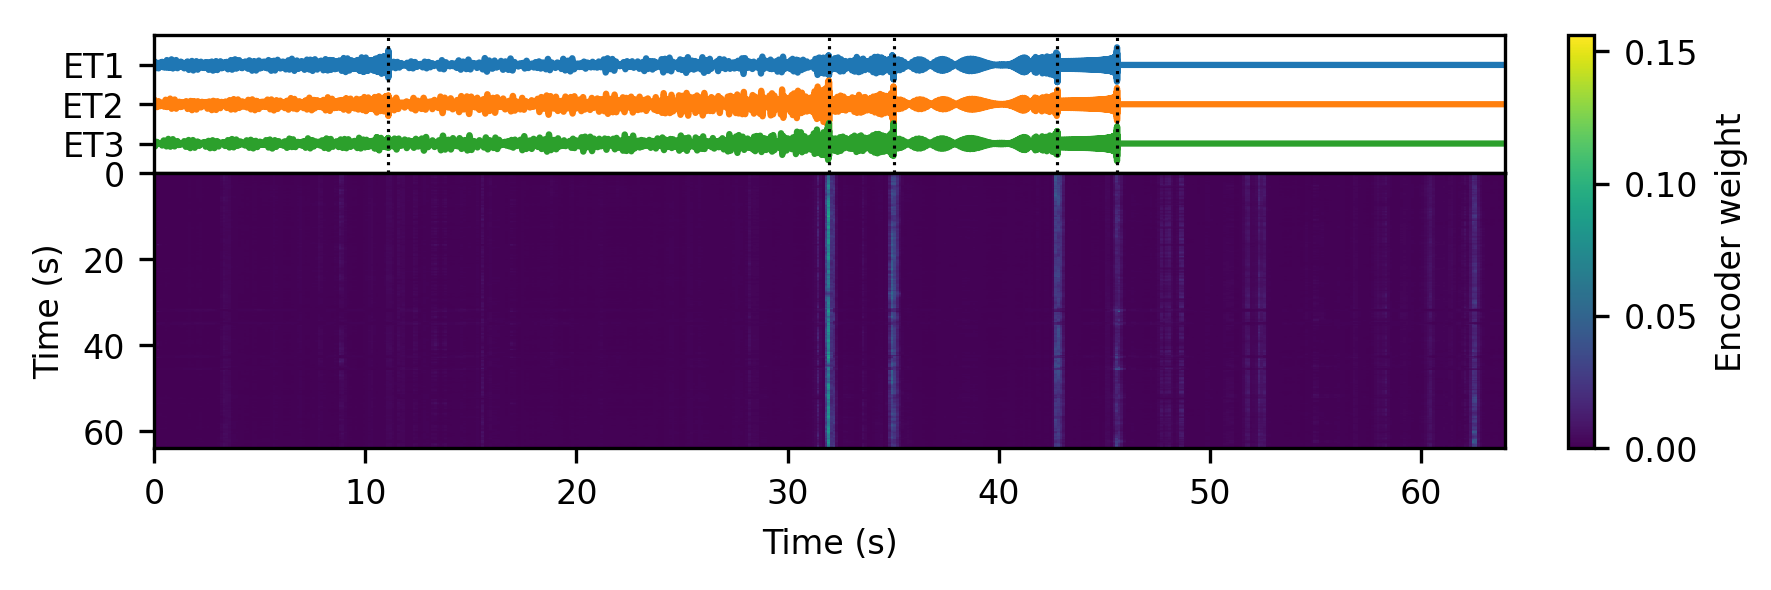
\includegraphics[
	width=15cm,
	trim=0 1cm 0 0,
	clip
	]{multiple_signal_detection/plots/weights/encoder/0}
	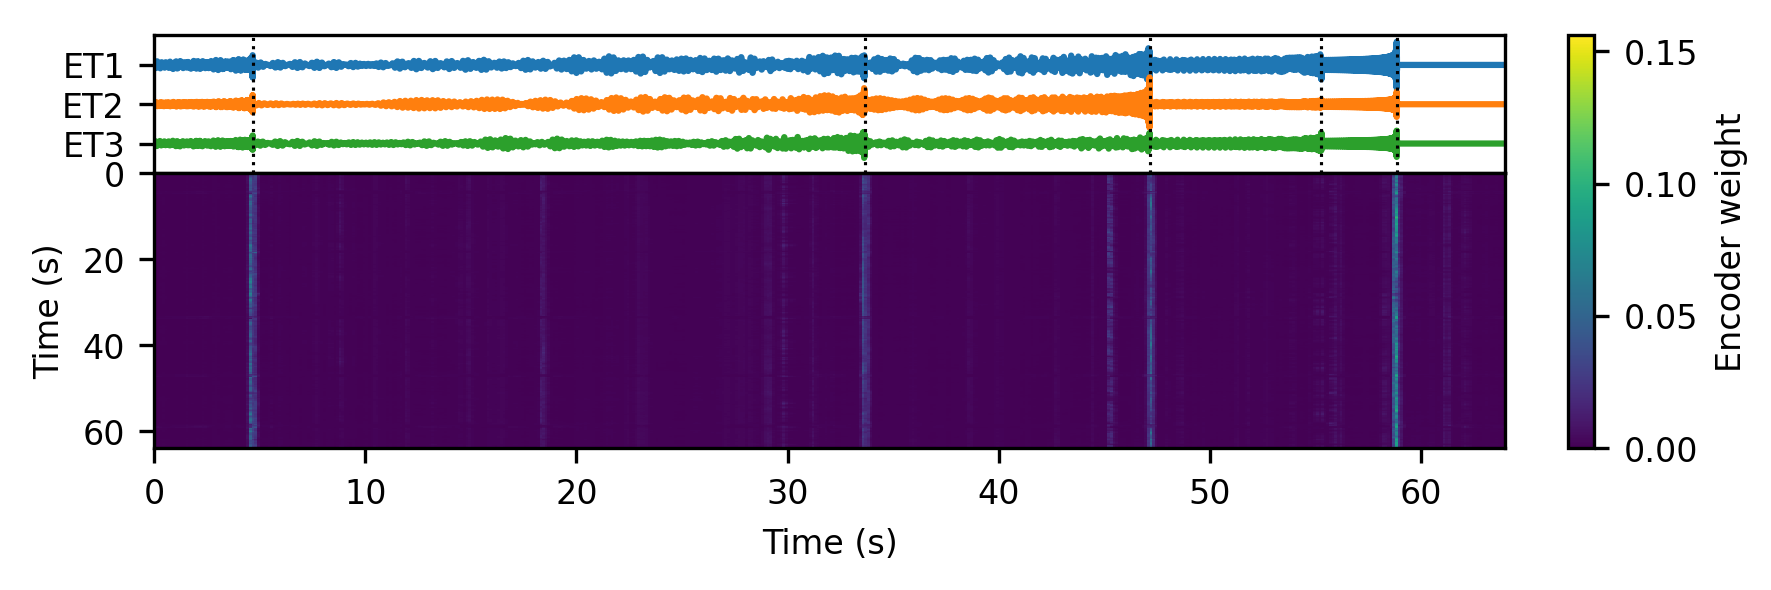
\includegraphics[
	width=15cm,
	]{multiple_signal_detection/plots/weights/encoder/8}
	\caption{Attention matrices of the transformer encoder model for five samples. Each of the $512$ tokens is assigned a time step. The x-axis shows the source sequence tokens and the y-axis the target sequence.}
	\label{fig:heatmap:encoder_weights}
\end{figure}

How the transformer makes use of its large receptive field can be investigated by plotting the encoder attention weights. See the last layer's weights averaged over all attention heads for five samples in Fig.~\ref{fig:heatmap:encoder_weights}. These examples suggest that tokens attend to the identified signals in a sample. It can be concluded that this global information is somehow helpful for making predictions, in high-overlap conditions especially, although it is not fully clear how. 

\section{Injection Study}

It has been seen that the difference in model performance between CNN and transformer encoder is associated with samples containing multiple signals. The results suggest that the CNN's $\approx\SI{1}{\second}$ receptive field is large enough to capture this overlap robustly, but the transformer's \emph{global} receptive field appears to improve performance when dealing with multiple signals per sample $n>1$.
The effect of time overlap is isolated for the case of two signals per sample, $n=2$. Here, according to Fig.~\ref{fig:heatmap:num_mergers}, the transformer encoder outperforms the CNN already with a detection ratio of \SI{63.8(2)}{\percent} compared to \SI{61.2(3)}{\percent}. In particular, model performance is checked against the coalescence-time separation between signals $\Delta t_\text{coa}$ in a controlled injection study. Denoting the two signals A and B, the time separation is defined as $\Delta t_\text{coa}=|t_\text{coa}^\text{A}-t_\text{coa}^\text{B}|$.

% effect of signal closeness on performance
% injection study: multiple datasets, each sample has exactly 2 signals. both injected at fixed times to ensure different delta ts between data sets
% we inject signal B always at 60s and signal A such that delta t is 30s, 10s, 3s, 1s, 0.6s, 0.3s, 0.2s, 0.1s
% these values are approximately logarithmic, with a higher resolution for dt<1s

For this, multiple \SI{66}{\kilo\nothing} sample test-datasets are simulated. What will be referred to as signal B is injected with a fixed coalescence time of \SI{60}{\second}, while signal A is injected at a time $<\SI{60}{\second}$. For each dataset, the signal A injection time is chosen to ensure a constant time separation. A total of eight datasets are simulated with separations of \SI{30}{\second}, \SI{10}{\second}, \SI{3}{\second}, \SI{1}{\second}, \SI{0.6}{\second}, \SI{0.3}{\second}, \SI{0.2}{\second} and \SI{0.1}{\second}. The values are chosen to be equidistant on a logarithmic scale with a higher resolution for $\Delta t_\text{coa}<\SI{1}{\second}$.

\begin{figure}
	\centering
	\makebox[\textwidth]{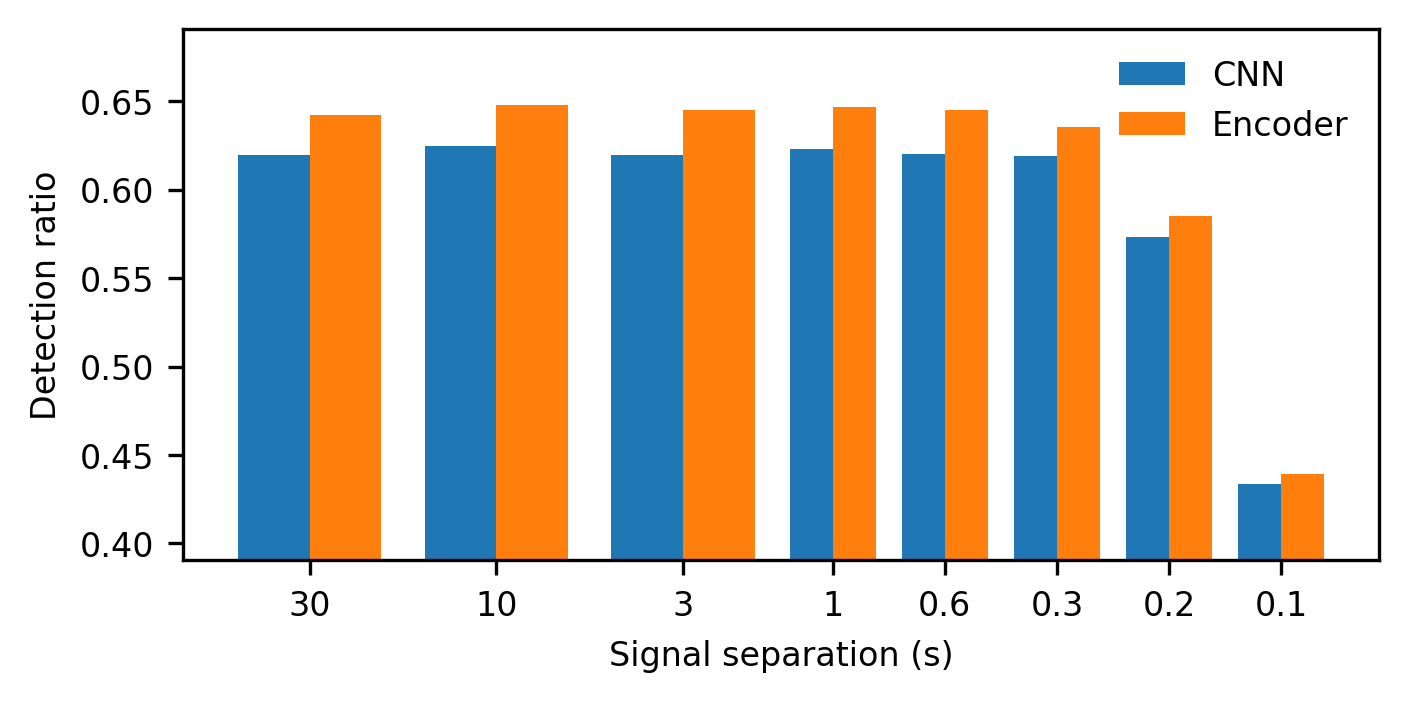
\includegraphics[width=12cm]{multiple_signal_detection/plots/cnn_encoder_deltat}}
	\caption{Detection ratio as a function of signal separation for the CNN (\emph{blue}) and the transformer encoder (\emph{orange}). Computed over \SI{66}{\kilo\nothing} samples with \SI{131}{\kilo\nothing} signals. Uncertainties are too small to be visualized.}
	\label{fig:heatmap:cnn_encoder_deltat}
\end{figure}

% plot detection ratio against signal separation
% two regimes: dt >= 0.3s, performance stays at 61% for cnn and 64% for encoder
% for dt < 0.3, both models degrade and the difference in performance becomes less noticable 
% from this it can be seen that the difference in performance stems not from close overlaps, rather from long range dependencies where the transformers global attention mechanism helps
% As a degradation in performance is noticable for both models once signals get close, it is reasonable to attribute this to the limited heatmap resolution (which is the same in both models)


For both models, the detection ratio is computed over each dataset separately. Assuming a binomial distribution, the uncertainties are $<\SI{0.14}{\percent}$. See the results in Fig.~\ref{fig:heatmap:cnn_encoder_deltat}. From this plot, two regimes can be identified. For $\Delta t_\text{coa} \geq \SI{0.6}{\second}$, model performance is agnostic to signal separation, varying by \SI{0.5(2)}{\percent} at most for the CNN and by \SI{0.6(2)}{\percent} for the encoder. The transformer encoder outperforms the CNN throughout this regime by $\approx\SI{3}{\percent}$. If $\Delta t_\text{coa} \leq \SI{0.3}{\second}$, both models degrade in performance, converging to similar detection ratios of \SI{43.3(1)}{\percent} and \SI{43.9(1)}{\percent}. 

Thus, the difference in model performance does not stem from close overlaps, but rather from long-range dependencies between signals, which are accessible to the transformer model through its global attention mechanism. For small $\Delta t_\text{coa}$, a similar performance decrease is noticeable in both models, suggesting a limitation shared by both architectures, which will be discussed later. 

% study allows for comparison to matched filtering
% \cite{Relton_2022} showed that without adaption matched filtering can handle overlapping signals 
% performance decrease for signals separated by less than 1s, where only one is retained
% see figure, 4 cases
% comparison to encoder model as it is better, this is quantitative only

\begin{figure}
	\centering
	\makebox[\textwidth]{\includegraphics[width=10cm]{multiple_signal_detection/images/delta_tc_stacked_FAR_labels_switched}}
	\caption{Matched-filtering performance as a function of signal separation \cite{Relton_2022}. Four cases are shown: only signal A is recovered (\emph{blue}), only signal B (\emph{red}), both signals (\emph{green}) or neither (\emph{grey}). A denotes the earlier signal.}
	\label{fig:heatmap:matched_filtering_deltat_cases}
\end{figure}

Fig.~\ref{fig:heatmap:cnn_encoder_deltat} shows that both models can detect signals with $\Delta t_\text{coa}\geq\SI{0.6}{\second}$ with no significant performance decrease. In contrast, according to \cite{Relton_2022}, standard matched-filtering searches degrade in performance for signals separated by $<\SI{1}{\second}$ already. In this regime, clustering routines cause only one of the two signals to be recovered. This injection study allows for a more direct comparison with matched filtering, as the methodology is similar to \cite{Relton_2022}. See their results in Fig.~\ref{fig:heatmap:matched_filtering_deltat_cases}. 
Because the exact datasets differ in signal parameters and SNRs and different FARs are employed, comparisons will be \emph{qualitative} only. 

\begin{figure}
	\centering
	\makebox[\textwidth]{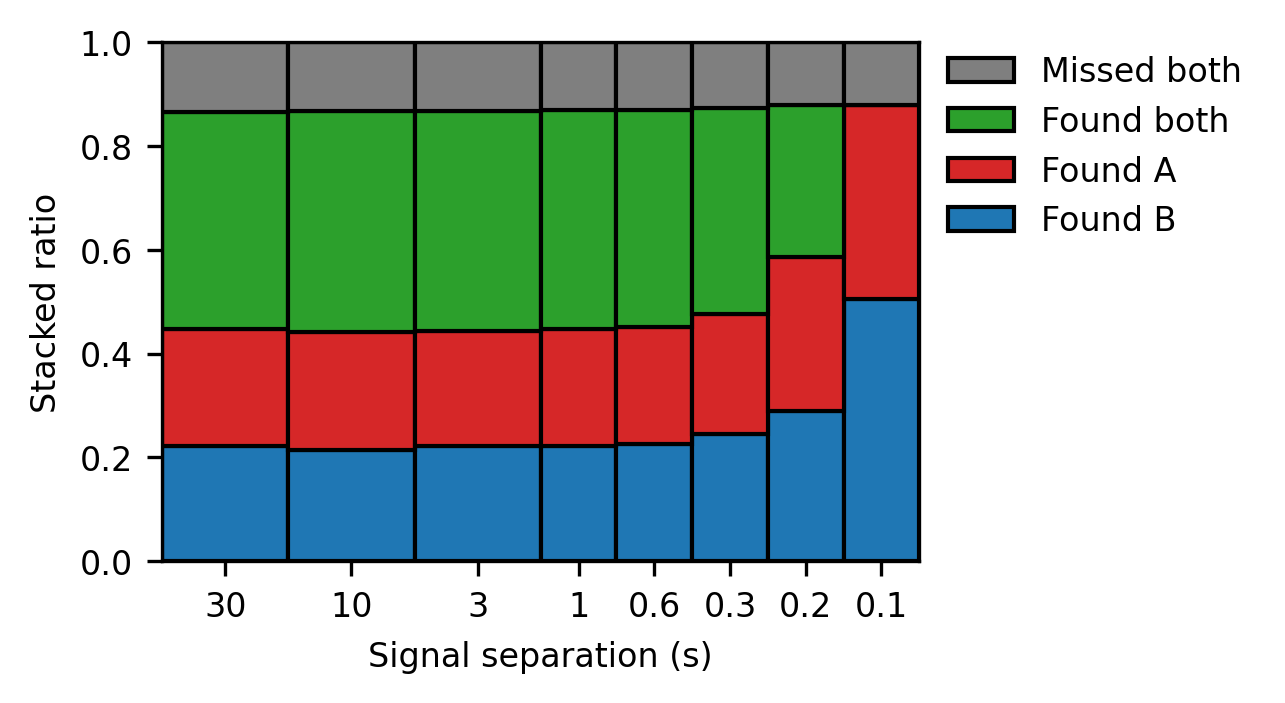
\includegraphics[width=11cm]{multiple_signal_detection/plots/encoder_stacked}}
	\caption{Transformer encoder performance with signal separation. For comparison with Fig.~\ref{fig:heatmap:matched_filtering_deltat_cases}, notice the different x-axis scale.}
	\label{fig:heatmap:encoder_deltat_cases}
\end{figure}

Fig.~\ref{fig:heatmap:matched_filtering_deltat_cases} is reproduced for the transformer encoder by distinguishing four cases: the model finds only signal A, only signal B, both signals or neither. Because comparisons are qualitative anyway, uncertainties are  simply neglected here. See the results in Fig.~\ref{fig:heatmap:encoder_deltat_cases}.
The plot shows that the model can distinguish signals up to separations of $\SI{0.2}{\second}$. At $\Delta t_\text{coa}=\SI{0.1}{\second}$, only one of two signals is recovered. Thus, at least qualitatively, the transformer encoder model is more robust than standard matched-filtering searches when handling close overlaps. 

\begin{figure}
	\centering
	\makebox[\textwidth]{
		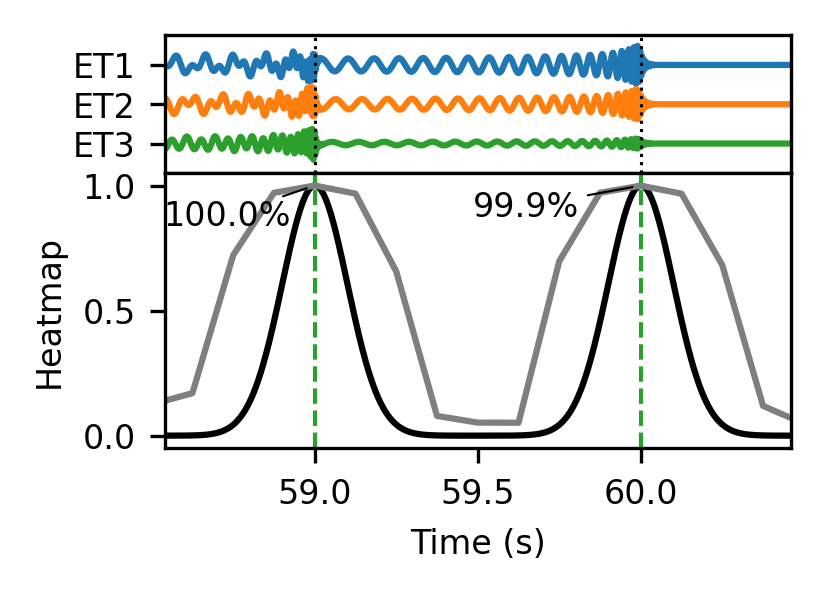
\includegraphics[
		height=5cm,
		trim=0 0 0 0,
		clip
		]{multiple_signal_detection/plots/out/700/encoder/0_zoom}
		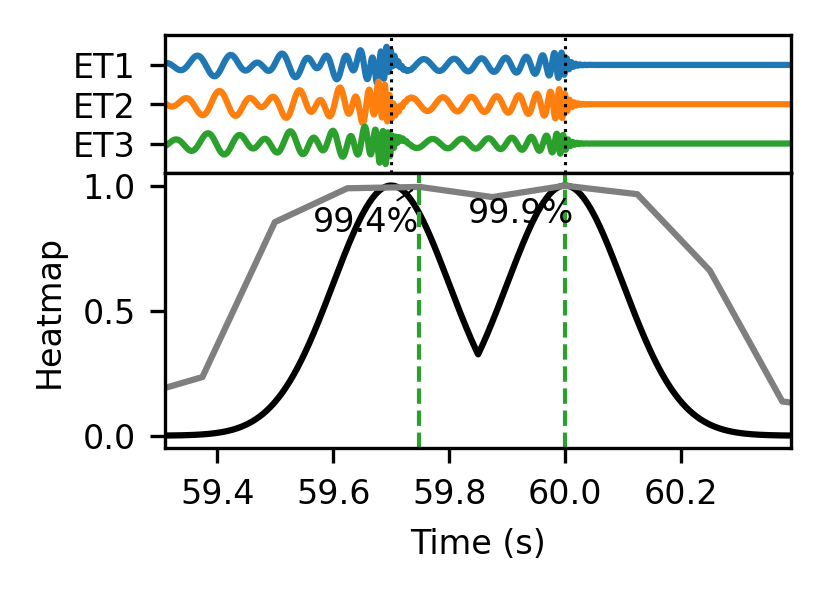
\includegraphics[
		height=5cm,
		trim=1.2cm 0 0 0,
		clip
		]{multiple_signal_detection/plots/out/800/encoder/7_zoom}
		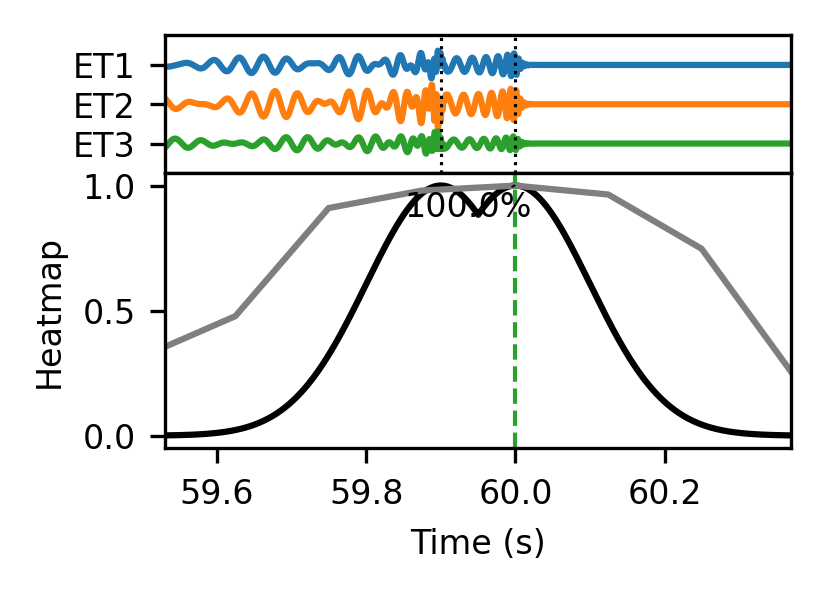
\includegraphics[
		height=5cm,
		trim=1.2cm 0 0 0,
		clip
		]{multiple_signal_detection/plots/out/900/encoder/6_zoom}
	}
	\caption{Three example ground-truth (\emph{black}) and predicted heatmaps (\emph{grey}) of the transformer encoder model for $\Delta t_\text{coa}=\SI{1}{\second}$ (\emph{left}), $\Delta t_\text{coa}=\SI{0.3}{\second}$ (\emph{middle}) and $\Delta t_\text{coa}=\SI{0.1}{\second}$ (\emph{right}).}
	\label{fig:heatmap:encoder_deltat_plot}
\end{figure}

As previous results suggest a limitation in both the CNN and encoder architectures for $\Delta t_\text{coa}\leq\SI{0.3}{\second}$, it is reasonable to attribute the performance decrease in this regime to the limited heatmap time resolution.  
Because of downsampling, heatmaps comprise $512$ time steps only, resulting in a sample time of \SI{0.125}{\second}. Thus, if two signals are separated by less than \emph{two} time steps, $\Delta t_\text{coa}<\SI{0.25}{\second}$, the resulting heatmap prediction can only produce one peak. See example ground-truth and predicted heatmaps in Fig.~\ref{fig:heatmap:encoder_deltat_plot}.

\section{Summary}

% heatmap regression for multiple overlapping signals

This chapter reformulated GW detection as a heatmap regression task. Adaptations have been made to the approach in previous research \cite{PhysRevD.100.063015} to reduce the number of post-processing steps and to handle multiple signals per sample.

% comparison of two models, one CNN (more standard) and one transformer (motivated by \cite{Papalini_2025})
% transformer outperforms CNN because it can handle long range dependencies through attention mechanism

Two architectures were investigated: a CNN and a transformer encoder, which were adapted from the binary-classification models introduced previously. Both achieved low FARs down to $1/\SI{}{\month}$ while retrieving a non-zero fraction of signals, with the transformer consistently outperforming the CNN.

An injection study showed that this advantage does not arise from resolving closely overlapping signals, but from exploiting long-range dependencies between multiple signals. Both architectures exhibited a common performance limit for signal separations $\leq\SI{0.3}{\second}$, consistent with the resolution of the predicted heatmaps. 

% models are better at handling close overlaps (qualitatively) than matched filtering
% struggle for dt<=0.3s because of heatmap resolution
% look into upsampling like unet?


\chapter{Detection Transformer}
\label{sec:detr}
% heatmap regression works
% limited by heatmap resolution
% adapt heatmap with upsampling (unet \cite{ronneberger2015unetconvolutionalnetworksbiomedical})?
% different approach -> forgoes heatmap limiation
% easily adapted to crude parameter estimation (important for low-latency searches), but this wont be covered here

The previous chapter showed that heatmap regression performs well for GW searches. However, the approach is limited by the time resolution of the output heatmap, which becomes problematic for close overlaps. 
One possible solution would be to increase the heatmap resolution, for example by adding \emph{upsampling} steps after the transformer encoder, similar to U-Net architectures \cite{ronneberger2015unetconvolutionalnetworksbiomedical}. 

In this chapter, a different approach is investigated, forgoing the heatmap approach entirely. Instead, a fully end-to-end model is developed: for a given sample, the model directly outputs multiple GW candidates, each with a signal score and time location. 
The approach is based on the Detection Transformer (DETR) \cite{10.1007/978-3-030-58452-8_13}, which was originally developed for object detection in images and is modified here to handle time series instead.
Although not implemented in this thesis, such a model can simply be adapted to return an estimate of the signal parameters as well, which is important for low-latency searches.

\section{Architecture}

\begin{figure}
	\centering
	\makebox[\textwidth]{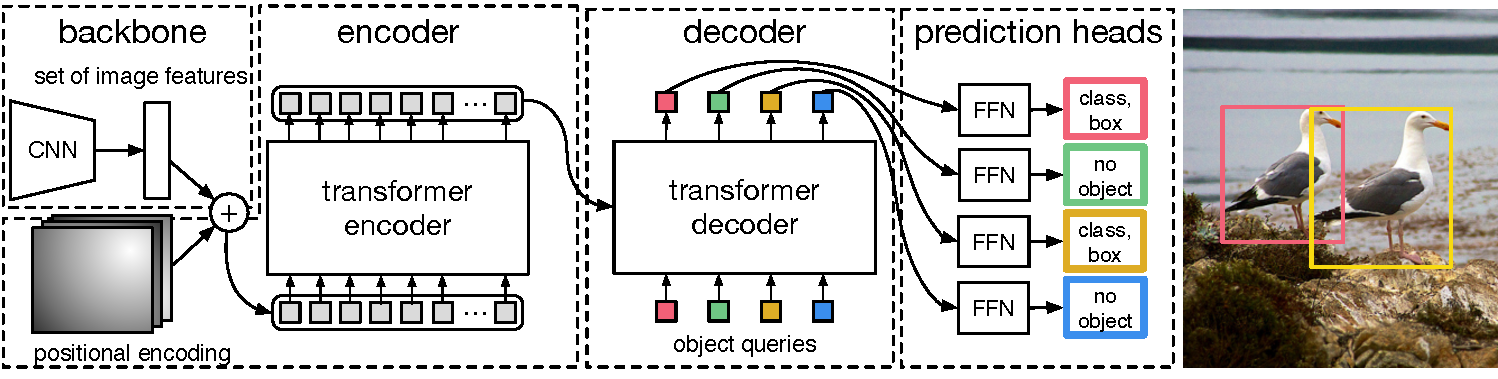
\includegraphics[width=16cm]{multiple_signal_detection/images/DETR_detail_seagulls}}
	\caption{Original DETR~\cite{10.1007/978-3-030-58452-8_13} architecture for image object detection. The model outputs multiple object class scores and bounding boxes.}
	\label{fig:detr:detr}
\end{figure}

\begin{figure}
	\centering
	\makebox[\textwidth]{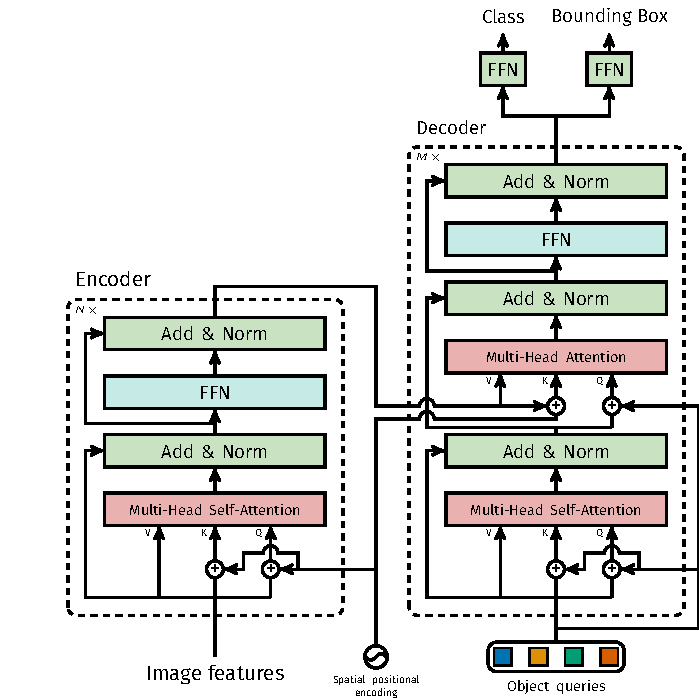
\includegraphics[width=11cm]{multiple_signal_detection/images/transformer}}
	\caption{Detailed implementation of the transformer used in DETR~\cite{10.1007/978-3-030-58452-8_13}. Positional encodings are not applied before the value projections.}
	\label{fig:detr:transformer}
\end{figure}

% explain architecture roughly see fig
% similar to transformer-encoder heatmap regressor
% instead of cls head transformer decoder (has been shown to improve performance)
% each query is read out via a cls and pos head + other parameters heads?

The DETR architecture consists of a CNN backbone, a transformer encoder, and a transformer decoder. Up to the encoder, the architecture is similar to the transformer-based heatmap-regressor. The difference is that the encoder output tokens are not read out directly to produce a heatmap, but serve as the source sequence of a transformer decoder. 
The decoder takes a number of learned \emph{queries} as its target sequence. The decoder output is read out with two prediction heads to produce a class score and the signal coalescence time. In principle, by appending more prediction heads, this architecture can be adapted to return other parameters as well.
See a schematic of the original architecture in Fig.~\ref{fig:detr:detr}. In a way, DETR is a natural extension of the ViT~\cite{DBLP:journals/corr/abs-2010-11929} architecture to multiple classification tokens.

One limitation of the DETR architecture is that the number of possible predictions per sample is fixed by the query count. This problem can be dealt with by simply choosing the number of queries to be sufficiently high. 

% details
% same CNN -> 512 tokens, 256 dim -> 64 embed dim
% transformer: 6 layers 8 heads
% encoder: sinusoidal, decoder: learned, only applied before q,k projections see fig
% decoder: 16 queries (refer to event rate)
% ff_dim = 1024, dropout = 0.1
% class head, time head
% \SI{6.2}{\mega\nothing} parameters, \SI{7}{\giga\byte}

For the CNN backbone, the same ResNet model as previously is employed. Given samples with a length of \SI{64}{\second}, the backbone outputs $512$ vectors of size $256$. A convolution operation with kernel size one projects these onto the embedding dimension $d_\text{embed}=64$. Both the transformer encoder and the decoder consist of six layers and eight heads, and employ FFNs with hidden dimension $d_\text{ff}=1024$. A dropout probability of \SI{10}{\percent} is used throughout the model. The transformer employs sinusoidal encodings for the encoder tokens and learned positional embeddings for the queries. Following the original architecture, these are applied before the query and key projections only (see Fig.~\ref{fig:detr:transformer}).

A total of $16$ queries is chosen. For the higher event-rate estimate of $\lambda=\SI{E+6}{\per\year}$, the probability for more than $16$ signals in a $T=\SI{64}{\second}$ long sample is negligible:
\begin{equation}
	P(n>16) = 1-\sum_{k=0}^{16}\,\frac{(\lambda T)^k}{k!}\,\e^{-\lambda T} = \SI{7E-9}{\percent},
\end{equation}
making this choice more than sufficient. These queries are learnable parameters of size $d_\text{embed}$, which are initialized as zero. After being passed through the decoder, each query is read out via two prediction heads.
The class score is obtained through,
\begin{equation}
\begin{aligned}
	n &= \mathrm{LayerNorm}(x),\\
	h &= \mathrm{ReLU}(\mathrm{Linear}_{64\rightarrow1024}(n)),\\
	z_c &=\mathrm{Linear}_{1024\rightarrow1}(h),
\end{aligned}
\end{equation}
which is later passed through a sigmoid layer. For the time prediction, the prediction head reads,
\begin{equation}
\begin{aligned}
	n &= \text{LayerNorm}(x),\\
	h_1 &= \text{ReLU}(\text{Linear}_{64\rightarrow1024}(n)),\\
	h_2 &= \text{ReLU}(\text{Linear}_{1024\rightarrow1024}(h_1)),\\
	h_3 &= \text{ReLU}(\text{Linear}_{1024\rightarrow1024}(h_2)),\\
	z_t &= \text{Linear}_{1024\rightarrow1}(h_3).
\end{aligned}
\end{equation}
This value is also passed through a sigmoid layer to normalize the prediction to $[0,1]$ in units of sample duration. In total, the network has \SI{6.2}{\mega\nothing} trainable parameters.

\section{Training}

\begin{figure}
	\centering
	\begin{minipage}{\textwidth}
	\centering
	\makebox[\textwidth]{
	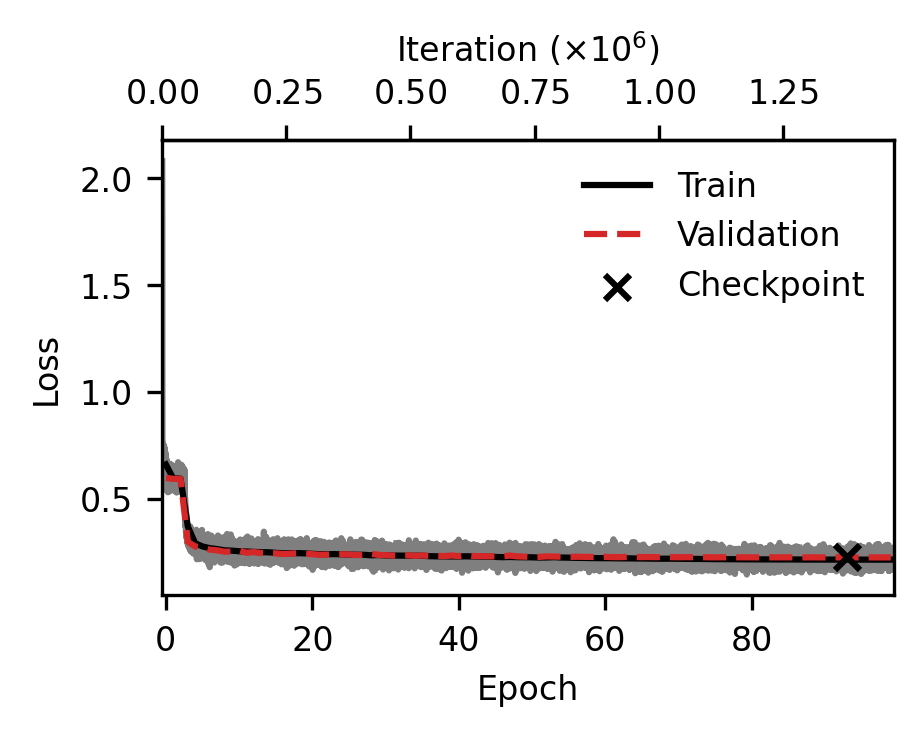
\includegraphics[width=8cm]{multiple_signal_detection/plots/learning_curves/detr_loss}
	}
	\caption{DETR learning curve. Total loss computed over the training dataset after each step (\emph{grey}) and averaged over each epoch (\emph{black}). Validation dataset loss (\emph{red}). The minimum validation-loss checkpoint is indicated.}
	\label{fig:detr:learning_curve}
	\end{minipage}
	\begin{minipage}{\textwidth}
	\centering
	\makebox[\textwidth]{
	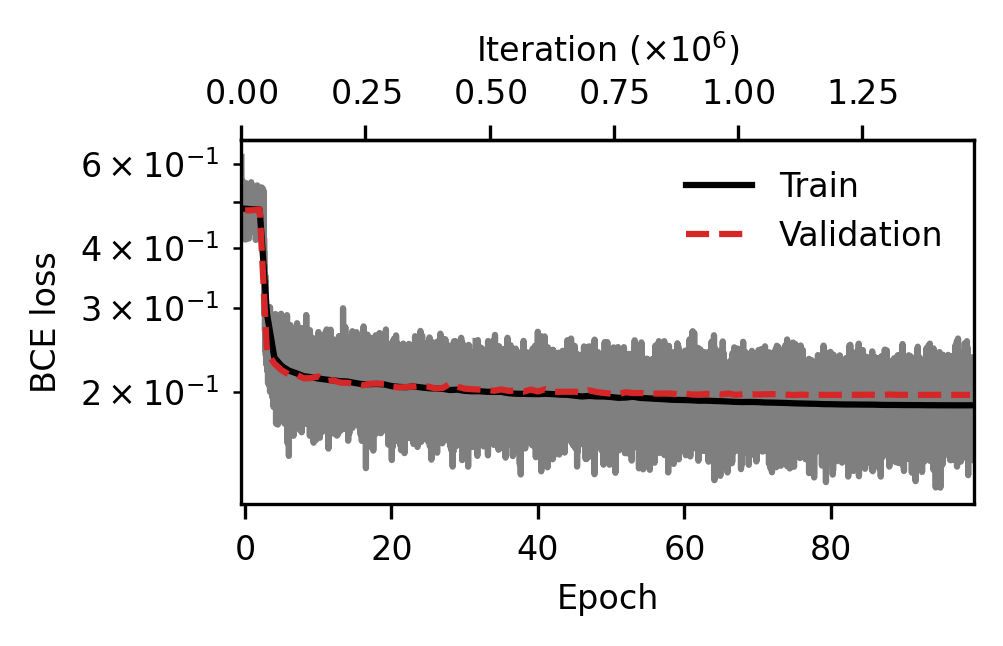
\includegraphics[width=8cm]{multiple_signal_detection/plots/learning_curves/detr_bce_loss}
	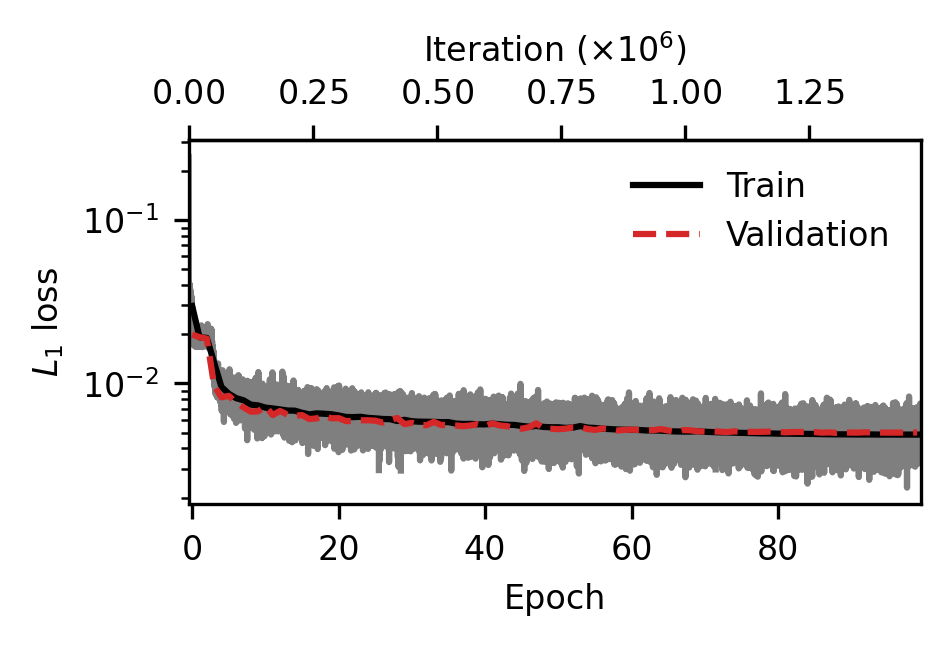
\includegraphics[width=8cm]{multiple_signal_detection/plots/learning_curves/detr_l1_loss}
	}
	\caption{Evolution of both loss terms during training. BCE loss (\emph{left}) and time prediction $L_1$ loss (\emph{right}).}
	\label{fig:detr:tandem}
	\end{minipage}
\end{figure}

%\begin{figure}
%	\centering
%	\makebox[\textwidth]{
%		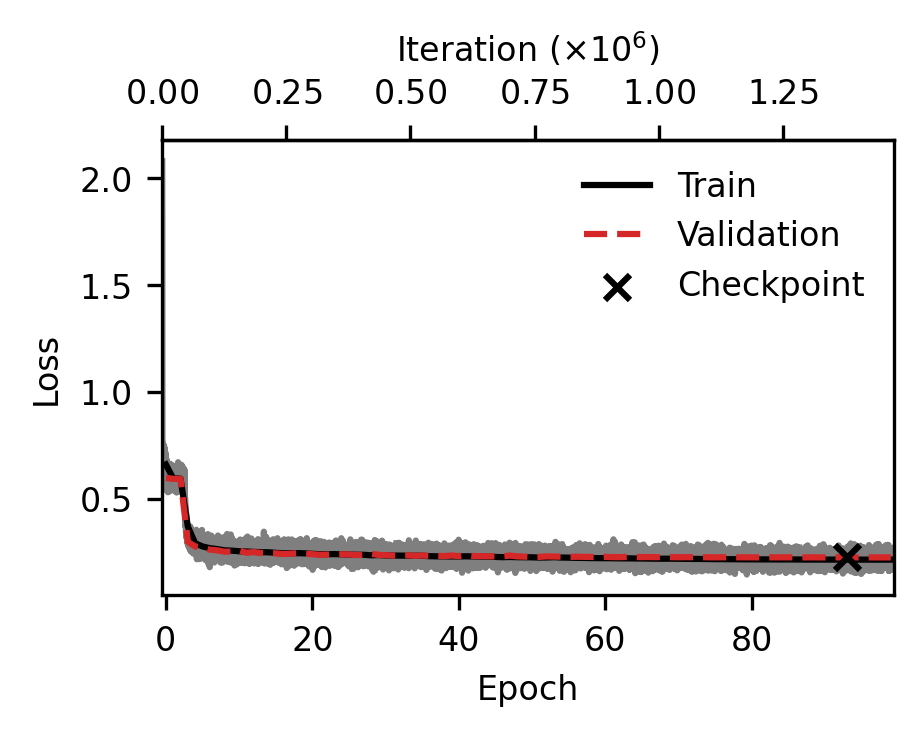
\includegraphics[width=8cm]{multiple_signal_detection/plots/learning_curves/detr_loss}
%	}
%	\caption{DETR learning curve. Total loss computed over the training dataset after each step (\emph{grey}) and averaged over each epoch (\emph{black}). Validation dataset loss (\emph{red}). The minimum validation-loss checkpoint is indicated.}
%	\label{fig:detr:learning_curve}
%\end{figure}
%\begin{figure}
%	\centering
%	\makebox[\textwidth]{
%		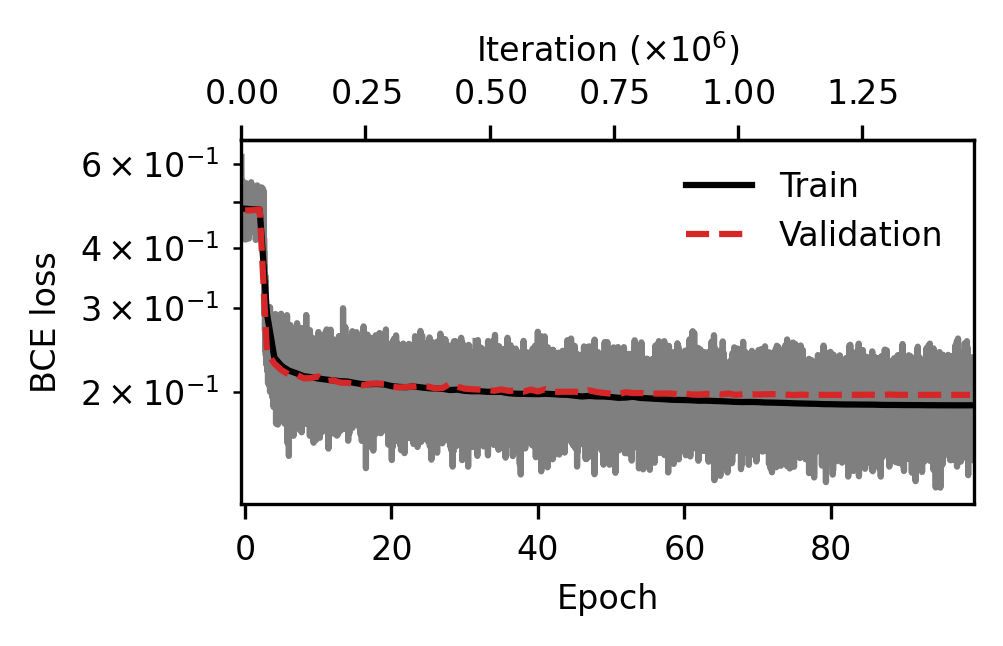
\includegraphics[width=8cm]{multiple_signal_detection/plots/learning_curves/detr_bce_loss}
%		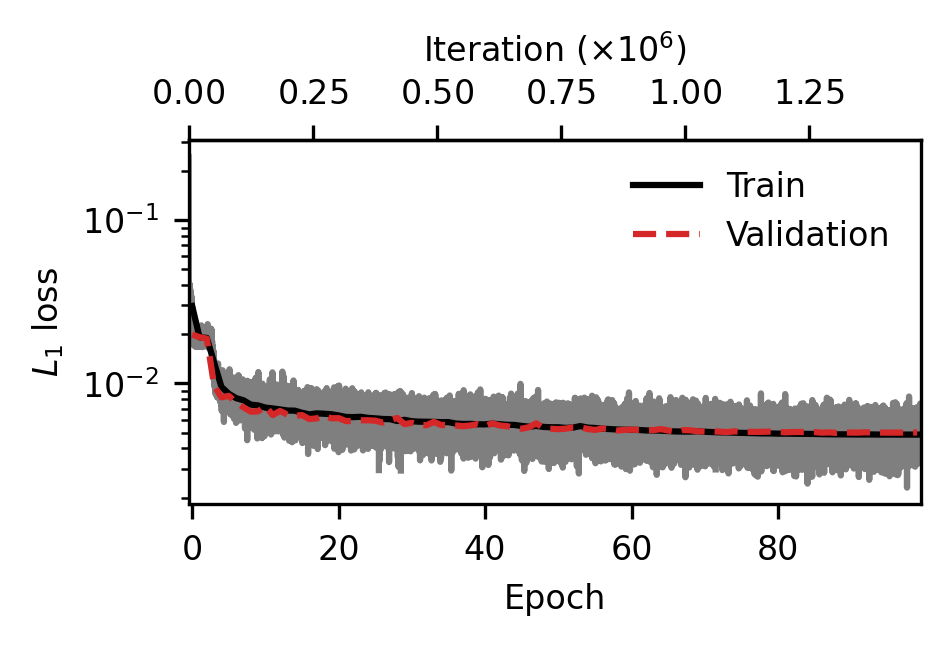
\includegraphics[width=8cm]{multiple_signal_detection/plots/learning_curves/detr_l1_loss}
%	}
%	\caption{Evolution of both loss terms during training. BCE loss (\emph{left}) and time prediction $L_1$ loss (\emph{right}).}
%	\label{fig:detr:tandem}
%\end{figure}

% loss function: train class and position in tandem 
% if c=0 time prediction is zeroed out
% what is the ground truth y?
% match m signals to m<n preds
% for unmatched preds the corresponding ground-truth is noise

For any given sample, the DETR architecture implemented here produces $m=16$ predictions $\hat{y}=\{(\hat{c}_j,\hat{t}_j)\}_{j=1}^{m}$, each comprising a signal score and coalescence time. The network is of course free to output predictions with $\hat{c}=0$, \emph{i.e.}\ noise predictions, which are discarded after thresholding. The class score and time prediction are trained in tandem, employing a BCE loss and an $L_1$ loss, summed over all predictions:
\begin{equation}
	\pazocal{L}(y, \hat{y}) = \sum_{j=1}^m \pazocal{L}_\text{BCE}(c_j, \hat{c}_j) + c_j\,\lambda|t_j - \hat{t}_j|.
\end{equation}
For predictions where the ground-truth class is noise, $c=0$, the time prediction loss is simply zeroed out. Since for random predictions the average BCE loss is $\pazocal{L}_\text{BCE}=\ln 2\approx0.69$, while the  $L_1$ loss to the nearest signal is only of order \SI{E-2}{}, the $L_1$ term is up-weighted by a factor $\lambda=6$. The exact value is chosen empirically.
The architecture makes use of \emph{auxiliary} losses, where the loss is computed over the output at each of the six decoder layers.

% how do we match? -> hungarian
% minimize total matching cost
% from this we get assignment function pi
% inverse gives indices i of signals matched to predictions j

Up to this point, it has been quietly swept under the rug what the ground truth $y=\{(c_j, t'_j)\}_{j=1}^{m}$ corresponding to the $m$ predictions actually looks like. 
For this purpose, all signals $\{t_i\}_{i=1}^{n}$ (where $n<m$) are assigned to predictions by a matching algorithm. Then the ground truth is constructed with
\begin{equation}
	\label{eq:detr:ground_truth}
	y_j = (c_j, t'_j) = \begin{cases}
		(1, t_i) & \text{if signal $i$ is matched to prediction $j$,} \\
		(0, \varnothing) & \text{else.}
	\end{cases}
\end{equation}
For unmatched predictions, the ground-truth coalescence time does not matter as the corresponding $L_1$ loss is zeroed out anyway.

Following \cite{10.1007/978-3-030-58452-8_13}, signals $i$ and predictions $j$ are matched by minimizing the cost,
\begin{equation}
	\pazocal{L}_\text{cost}(t_i, \hat{y}_j) = -\hat{c}_j + \lambda|t_i-\hat{t}_j|,
\end{equation}
where again $\lambda=6$.
Let $\tau:\pazocal{I}\rightarrow\pazocal{J}'$ denote an \emph{assignment function} mapping the signal indices $\pazocal{I} = \{1, 2, \dots, n\}$ to the subset of matched prediction indices $\pazocal{J}' \subset\pazocal{J} = \{1, 2, \dots, m\}$. The \emph{optimal} assignment function $\pi$ will be the realization of $\tau$ that minimizes the total assignment cost over all signals $i$ and corresponding predictions $\tau(i)$:
\begin{equation}
	\pi = \argmin_\tau \sum_{i=1}^n \pazocal{L}_\text{cost}(t_i, \hat{y}_{\tau(i)}).
\end{equation}
This is referred to as an \emph{assignment problem} and can be solved with methods implemented by SciPy \cite{2020SciPy-NMeth}. 

It can be seen that the index $i$ of a signal that is matched to a prediction $j$ is given by $\pi^{-1}(j)$. This function $\pi^{-1}(j)$ is only defined for those predictions $j$, which have been matched, $j\in\pazocal{J}'$. Thus with Eq.~\ref{eq:detr:ground_truth}, the ground truth $y_j$ that corresponds to $\hat{y}_j$ can be constructed as,
\begin{equation}
	y_j = \begin{cases}
		(1, t_{\pi^{-1}(j)}) & \text{if $j\in\pazocal{J}'$,} \\
		(0, \varnothing) & \text{else.}
	\end{cases}
\end{equation}
To differentiate this scheme from greedy matching, which is used for evaluation, the matching algorithm here will be referred to as \emph{Hungarian matching} following the terminology in \cite{10.1007/978-3-030-58452-8_13}.

% adamw with lr e-4, lam e-4, for a maximum of 100 epochs
% vram = 7gib, check maybe?
% cosine annealing with 5000 steps warmup

The DETR model is trained on the same \SI{1}{\mega\nothing} sample dataset as the heatmap models. The AdamW optimizer is used with a learning rate of \SI{E-4}{}, a weight decay of \SI{E-4}{} and a batch size of $64$. Training is performed for a maximum of $100$ epochs. For this, a cosine-annealing learning-rate schedule is employed with a warmup of $5000$ steps. 

See the total loss learning curve in Fig.~\ref{fig:detr:learning_curve}. The validation loss reaches its minimum after $93$ epochs. This checkpoint is used for all following results. Fig.~\ref{fig:detr:tandem} shows the evolution of the individual loss terms. It can be seen that both the class score and the time prediction have been successfully optimized in tandem. 

\section{Comparison with Heatmap Regression}

\begin{figure}
	\centering
	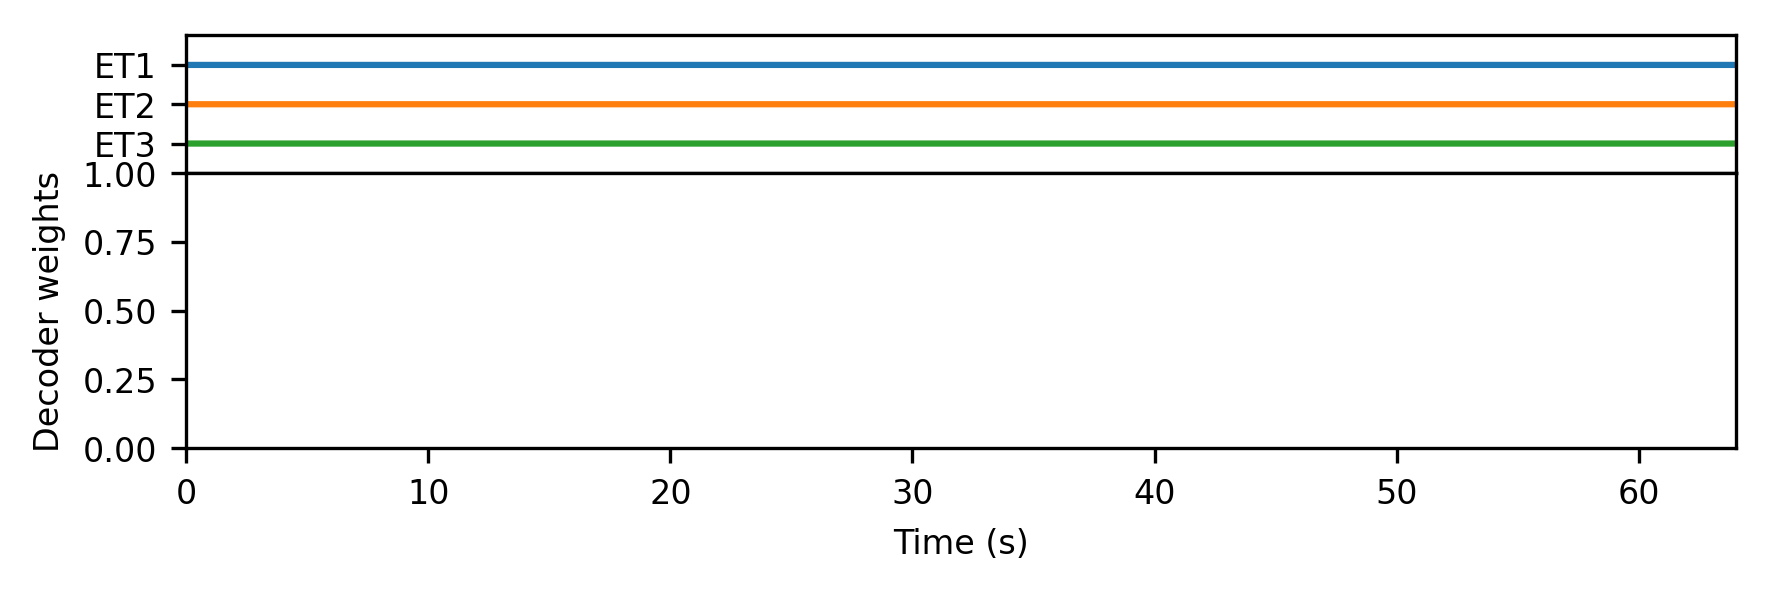
\includegraphics[
	width=15cm,
	trim=0 1cm 0 0,
	clip
	]{multiple_signal_detection/plots/out/300/detr/11}
	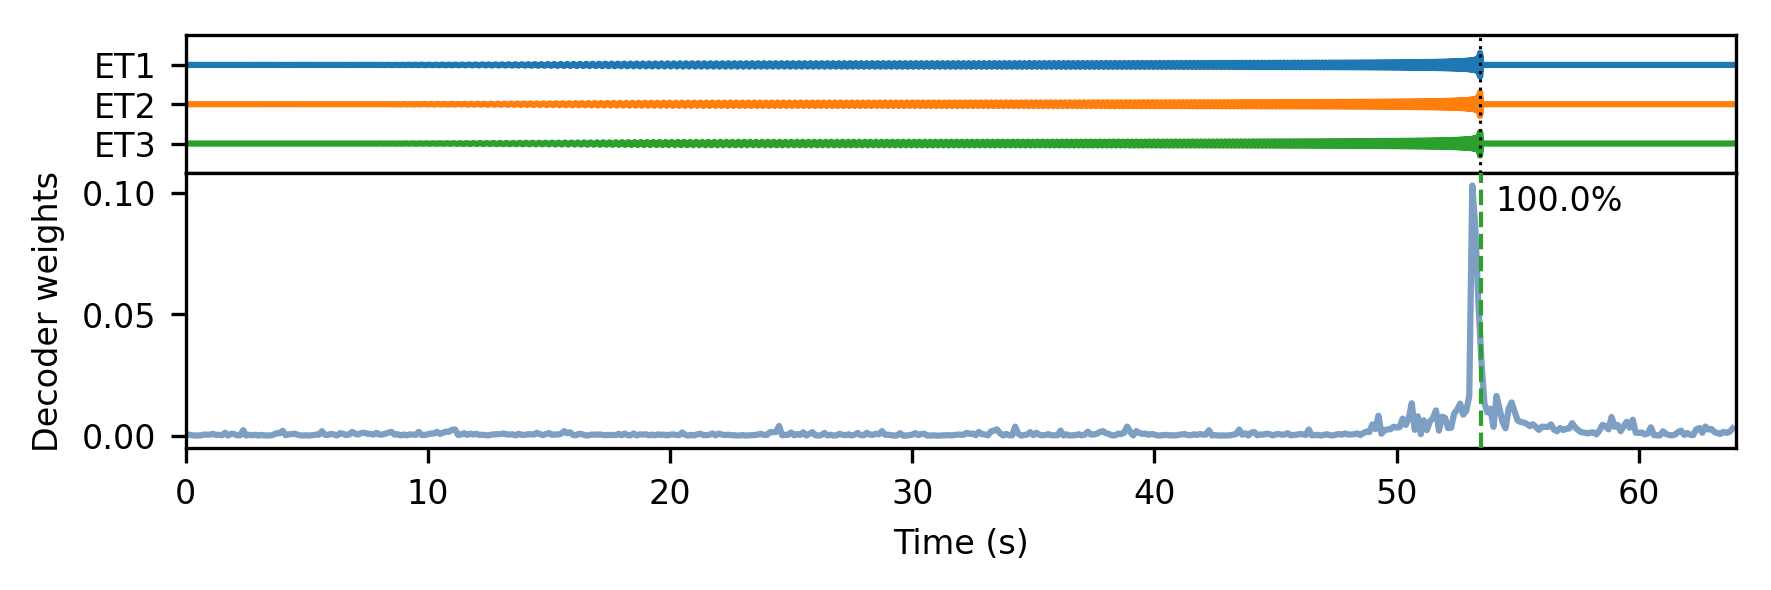
\includegraphics[
	width=15cm,
	trim=0 1cm 0 0,
	clip
	]{multiple_signal_detection/plots/out/300/detr/1}
	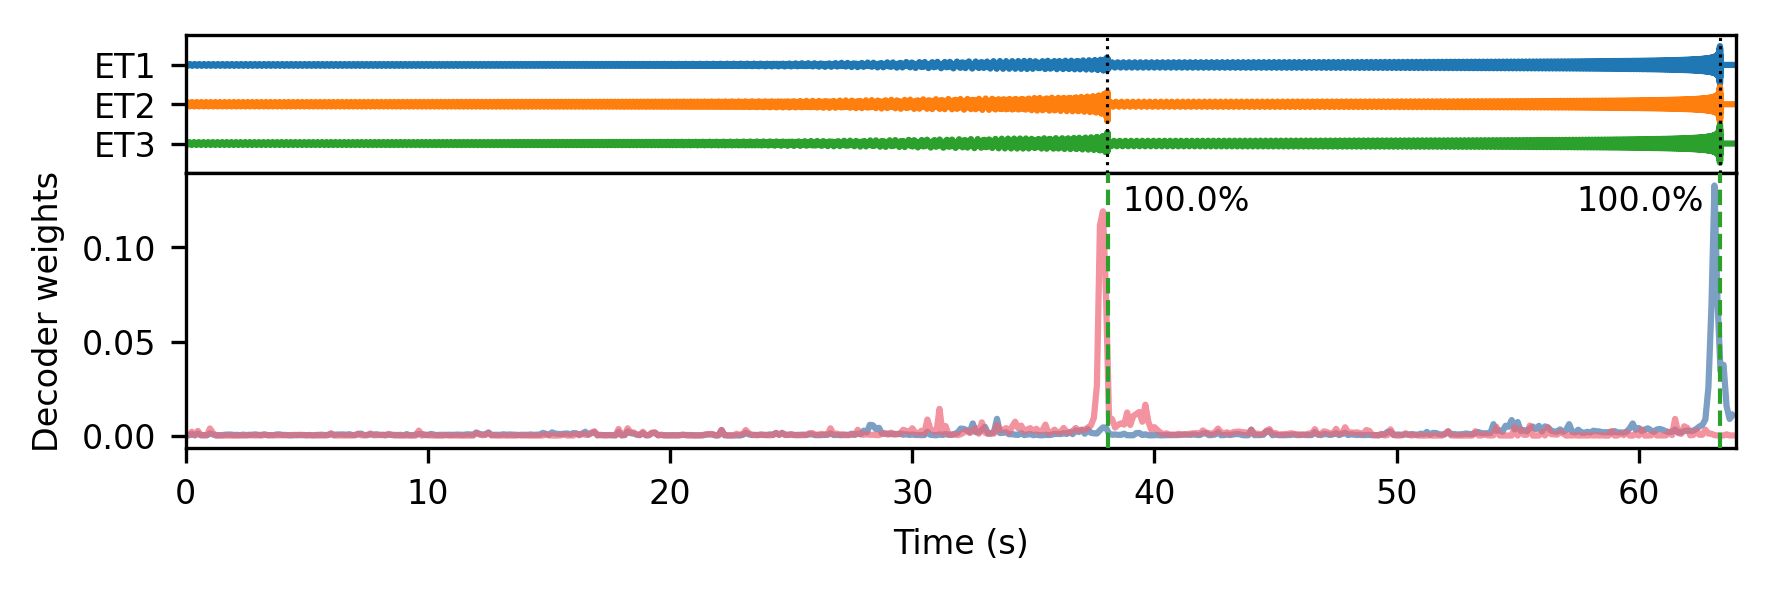
\includegraphics[
	width=15cm,
	trim=0 1cm 0 0,
	clip
	]{multiple_signal_detection/plots/out/300/detr/3}
	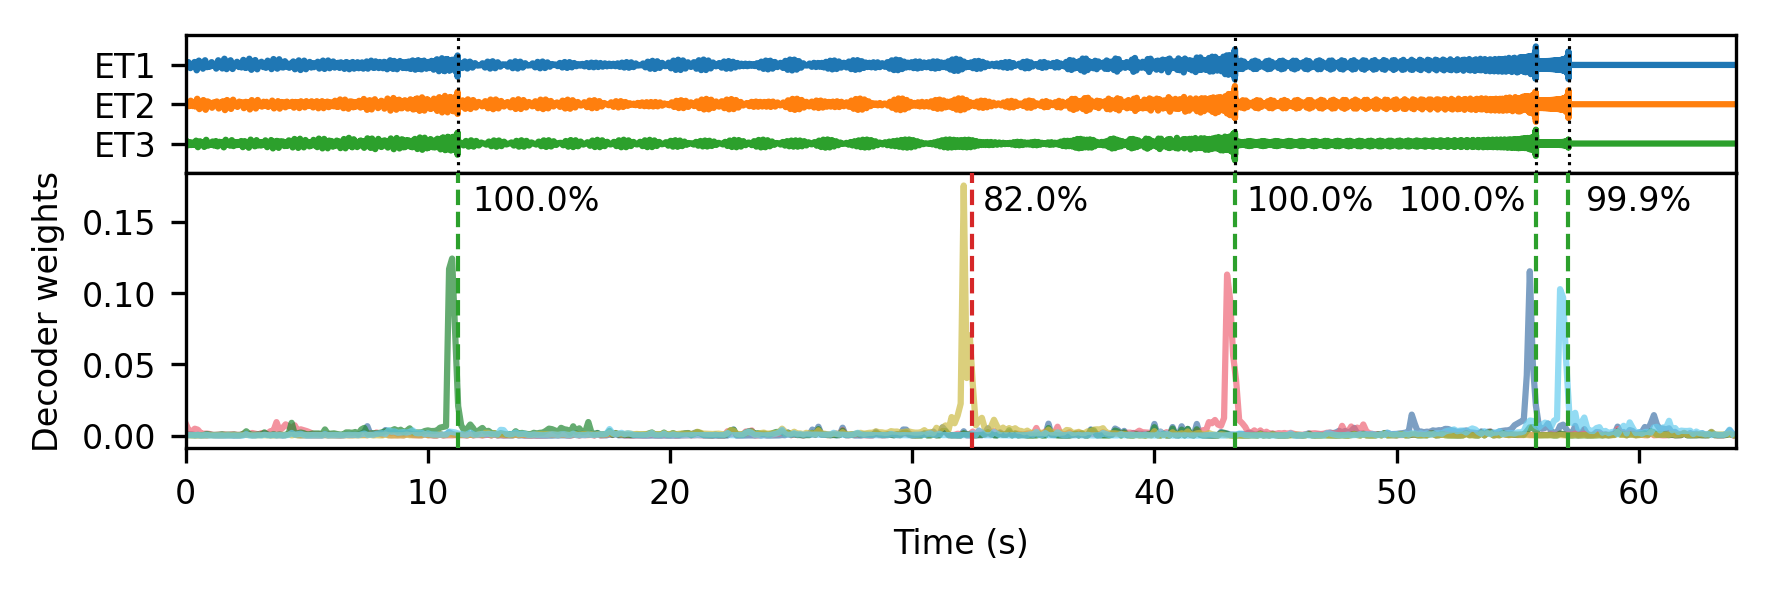
\includegraphics[
	width=15cm,
	trim=0 1cm 0 0,
	clip
	]{multiple_signal_detection/plots/out/300/detr/0}
	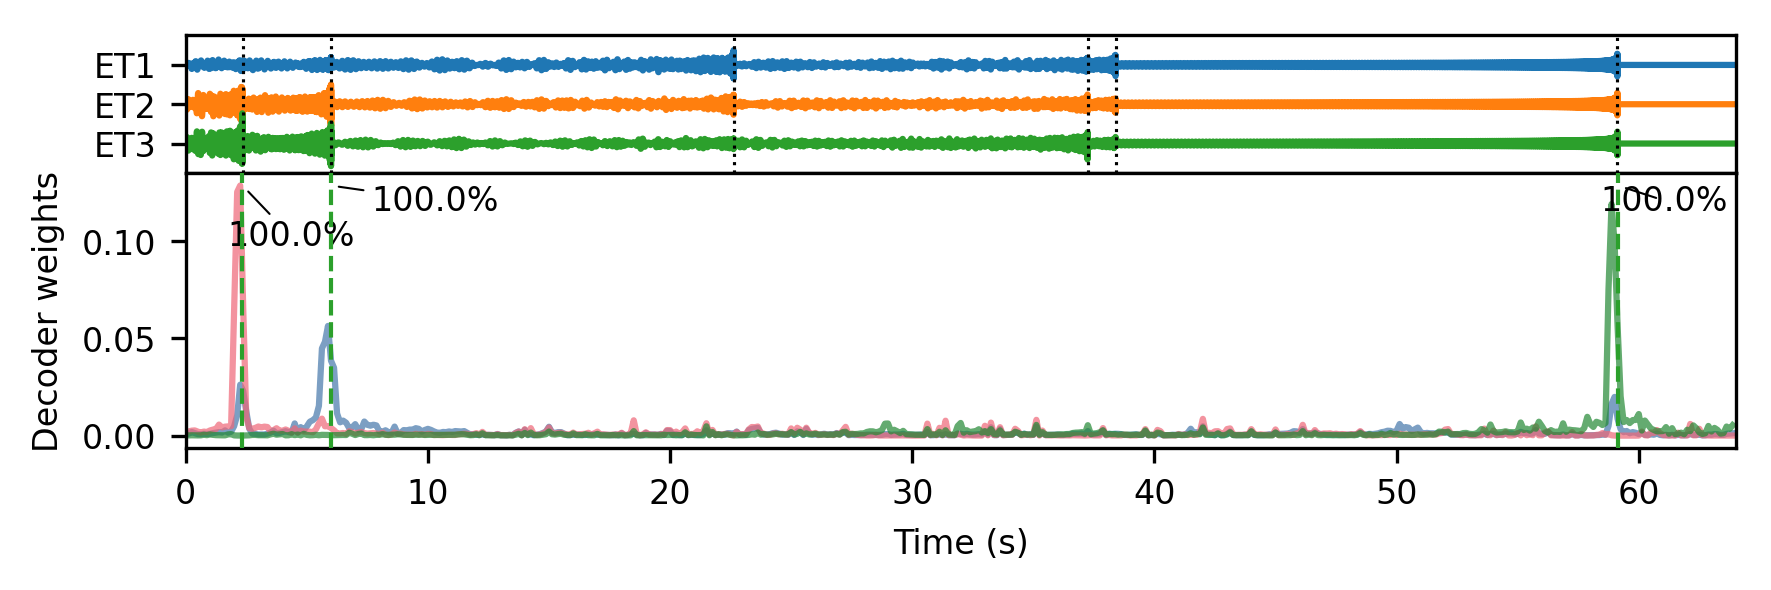
\includegraphics[
	width=15cm,
	]{multiple_signal_detection/plots/out/300/detr/8}
	\caption{DETR output for five samples. Each query is a GW candidate. These are plotted in the same manner as in Fig.~\ref{fig:heatmap:encoder_out}, and only candidates with scores exceeding \SI{69}{\percent} are shown. For each prediction, query--time cross-attention is plotted in different colors.}
	\label{fig:detr:out}
\end{figure}

% look at examples
% queries produce meaningful gw candidates
% choosing a threshold of 69%, FPs are rather low, while GW can be retrieved
% queries attend to time series through cross attention
% each query focuses on one signal

The following results and discussion largely mirror the structure of the previous chapter. The DETR model is evaluated on the same \SI{131}{\kilo\nothing}-sample test dataset, and GW candidates are assigned to signals with greedy matching. See the methodology in  Ch.~\ref{sec:heatmap:setup}.

It is again insightful to first inspect individual model outputs. See five examples in Fig.~\ref{fig:detr:out}. It can be seen that the DETR queries produce meaningful GW candidates. By applying a class-score threshold of \SI{69}{\percent}, most signals can be retrieved while keeping the number of FPs small. The choice of this threshold is justified later on. The predicted coalescence times also appear sufficiently accurate for the matching criterion $|t-\hat{t}|\leq\SI{0.1}{\second}$ used in this work.

The DETR prediction queries can attend to the time series through cross-attention.
The plots in Fig.~\ref{fig:detr:out} indicate that each query focuses mostly on a localized region of the input, close to the corresponding signal coalescence time.

\begin{figure}
	\centering
	\makebox[\textwidth]{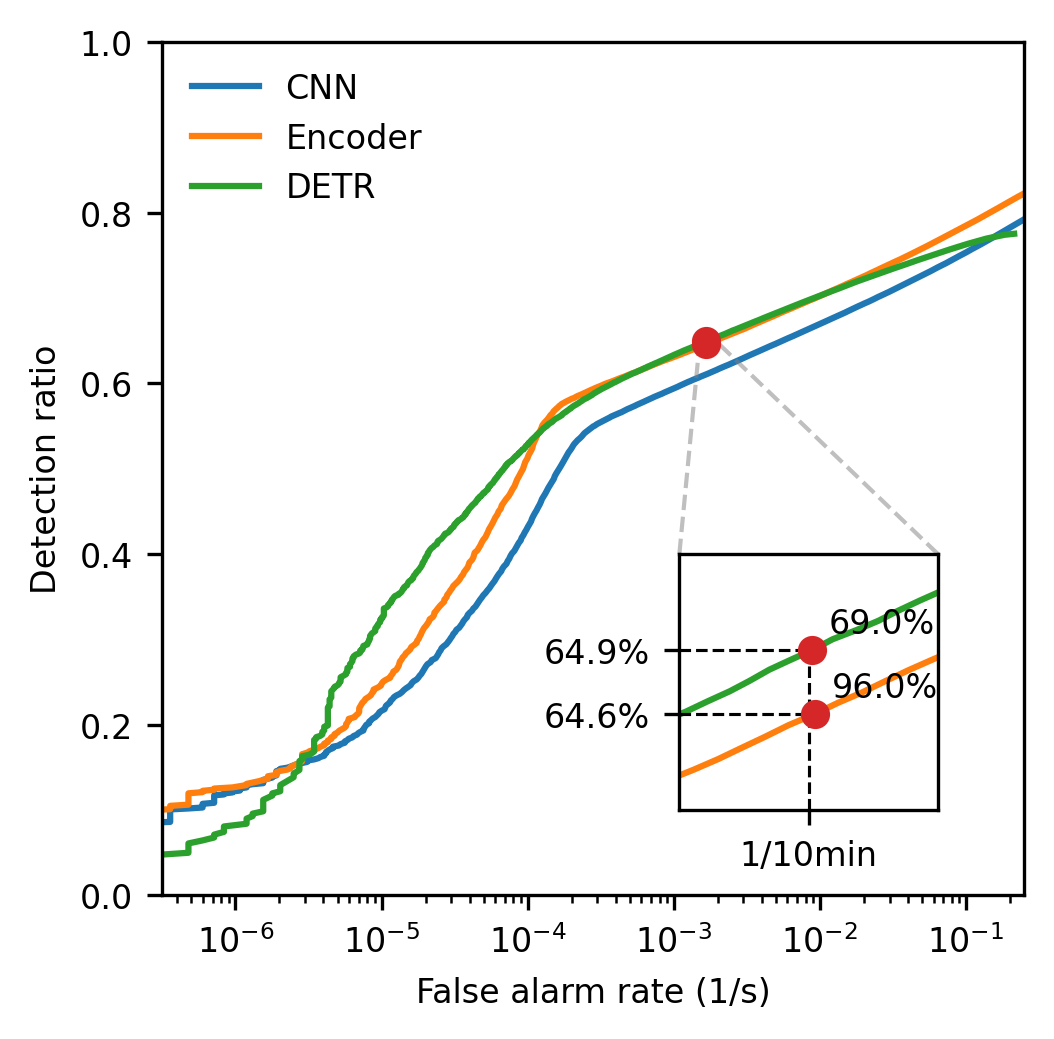
\includegraphics[width=9cm]{multiple_signal_detection/plots/cnn_encoder_detr_far}}
	\caption{Detection ratio as a function of FAR for the CNN heatmap regressor (\emph{blue}), transformer-encoder heatmap regressor (\emph{orange}), and DETR model (\emph{green}).}
	\label{fig:detr:far}
\end{figure}

% Performance comparison -> detection ratio against FAR
% see fig
% for high fars very similar to encoder
% for 10^-4<far<10^-5 -- 10^-6 better
% for really low far worse than both heatmap regressors
% comparable or even better performance that Encoder heatmap regressors while removing the need for postprocessing
% for low far performance maybe finetune with greedy matching

A quantitative comparison is obtained by varying the score threshold and computing the detection ratio and FAR over the full test dataset. Figure~\ref{fig:detr:far} compares the resulting operating characteristic of DETR with both heatmap regressors from the previous chapter. Over a large part of the FAR range, DETR performs comparably to the transformer heatmap model. For FARs from $\approx\SI{E-4}{\per\second}$ down to values between $\SI{E-5}{\per\second}$ and $\SI{E-6}{\per\second}$, DETR even reaches a higher detection ratio. At the lowest FARs, however, DETR falls below both heatmap regressors.

% TODO: DETR value was guessed in the 2nd nachkommastelle
At the fixed FAR operating point of $1/\SI{10}{\minute}$, DETR reaches a similar detection ratio of \SI{64.90(8)}{\percent}, compared to \SI{64.61(8)}{\percent} for the transformer-encoder heatmap regressor. The corresponding score threshold is \SI{69.0}{\percent}. Thus, DETR achieves comparable performance to heatmap regression while directly producing candidate scores and times, without requiring any post-processing steps.

\begin{figure}
	\centering
	\makebox[\textwidth]{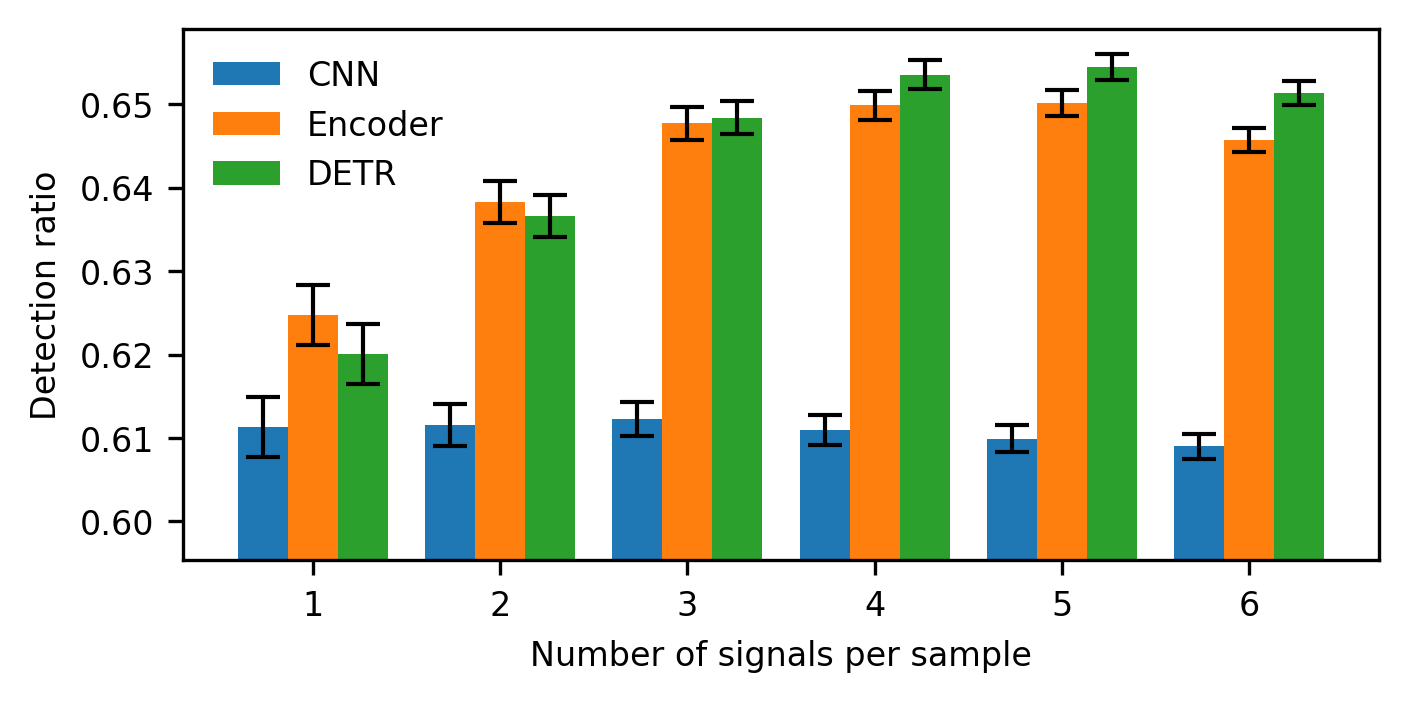
\includegraphics[width=12cm]{multiple_signal_detection/plots/cnn_encoder_detr_mergers}}
	\caption{Detection ratio as a function of the number of mergers per sample $n$. CNN heatmap regressor (\emph{blue}), transformer-encoder heatmap regressor (\emph{orange}), and DETR model (\emph{green}).}
	\label{fig:detr:num_mergers}
\end{figure}

% by looking at the performance with the number of mergers the same performance increase for samples with many signals can be observed
% because its also a transformer network and can exploit global information

The dependence on the number of signals per sample is shown in Fig.~\ref{fig:detr:num_mergers}. For $n=1$, DETR reaches comparable performance to the other models. Similar to the transformer-encoder heatmap regressor, DETR improves for larger $n$ as the detection ratio increases by \SI{3.4(4)}{\percent}.
This is consistent with DETR's use of global attention, which already appeared advantageous in the transformer heatmap regressor.

\begin{figure}
	\centering
	\makebox[\textwidth][c]{
		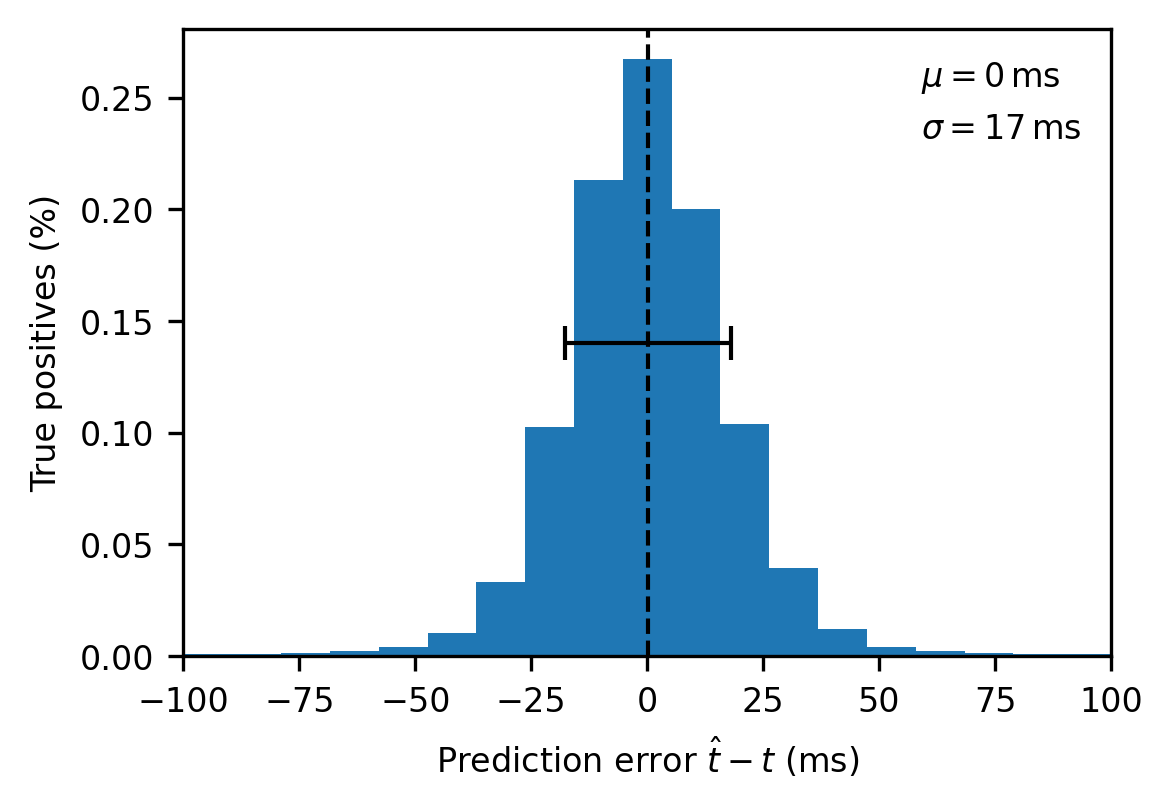
\includegraphics[width=8cm]{multiple_signal_detection/plots/detr_time}
		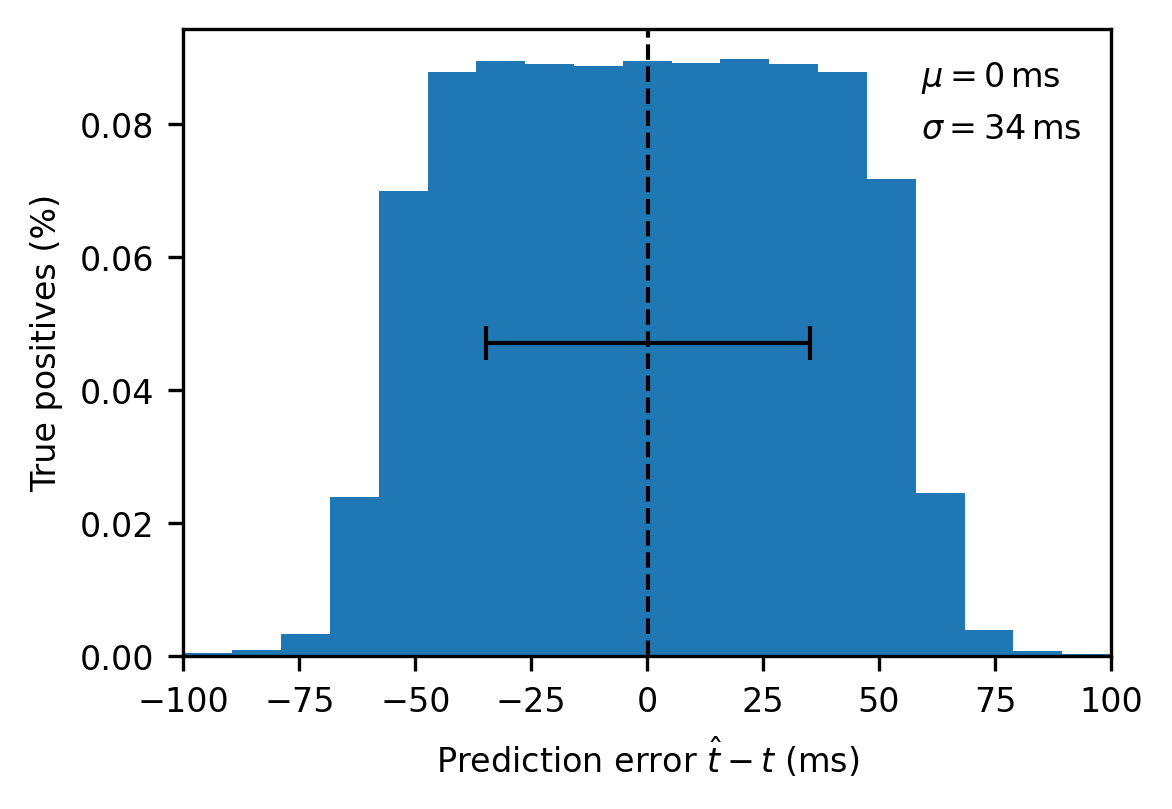
\includegraphics[width=8cm]{multiple_signal_detection/plots/encoder_time}
	}
	\caption{Prediction time error $\hat{t}-t$ for DETR (\emph{left}) and the transformer heatmap-regressor (\emph{right}). A vertical line shows the distribution mean $\mu$ and an error bar the standard deviation $\sigma$. The x-axis limits correspond to the matching criterion $|t-\hat{t}|\leq\SI{0.1}{\second}$.}
	\label{fig:detr:encoder_detr_time_acc}
\end{figure}

An important difference between DETR and heatmap regression is the way coalescence times are predicted. In heatmap regression, predictions are obtained by peak extraction and a local soft-argmax, while DETR predicts coalescence times directly. The effect on prediction time-accuracy is investigated by computing the error $\hat t - t$ for all TP predictions. 
The errors are plotted as histograms for both models in Fig.~\ref{fig:detr:encoder_detr_time_acc}.

% look at time prediction accuracy
% much better than encoder heatmap
% compute mean and std

Both error distributions have zero mean. For DETR, the distribution is sharper with a standard deviation of \SI{17}{\milli\second} compared to \SI{34}{\milli\second} for the heatmap regressor. Thus, DETR improves the time-prediction accuracy.

\section{Injection Study}

% no limitation because of heatmap resolution and better time accuracy -> probably better at close mergers

The previous chapter showed that heatmap regression becomes limited for nearby signals with $\Delta t_\text{coa}\leq\SI{0.3}{\second}$, as the two heatmap peaks can no longer be distinguished. Since DETR predicts coalescence times directly, one might expect improved performance for close overlaps. To test this, the same two-signal injection study as in the previous chapter is repeated for DETR.

\begin{figure}
	\centering
	\makebox[\textwidth]{
		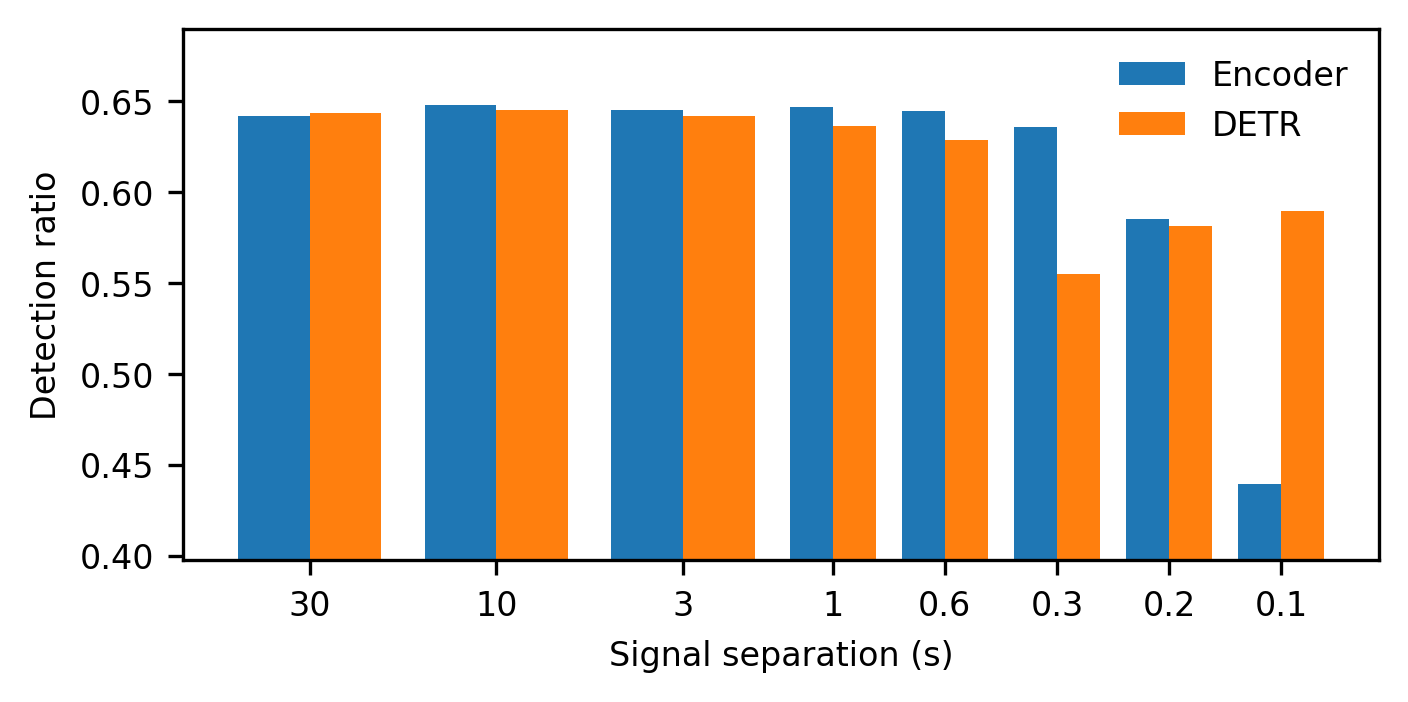
\includegraphics[width=12cm]{multiple_signal_detection/plots/encoder_detr_deltat}
	}
	\caption{Detection ratio as a function of signal separation for the transformer-encoder heatmap regressor (\emph{blue}) and for DETR (\emph{orange}). Computed over \SI{66}{\kilo\nothing} samples with \SI{131}{\kilo\nothing} signals. Uncertainties are too small to be visualized.}
	\label{fig:detr:detr_deltat}
\end{figure}

% do the same plot as before (see fig)
% network retains performance although it seems to be less robust than heatmap
% intermediate regime: worse?
% close regime: better because not limited

Fig.~\ref{fig:detr:detr_deltat} shows the detection ratio as a function of coalescence-time separation. The plot shows that, for separations $\geq\SI{3}{\second}$, both models perform equally well. DETR exhibits a performance decrease for separations of $\leq\SI{1}{\second}$ compared to $\leq\SI{0.3}{\second}$ for the heatmap regressor. However, this decrease is less pronounced for close separations of $\SI{0.1}{\second}$, where DETR retains a detection ratio of \SI{59.0(1)}{\percent} compared to \SI{43.9(1)}{\percent}. 

% look at delta t cases
% can predict multiple signals regardless of dt
% it does seem to struggle identifying signals if they are close
% especially in the strong regime dt<1s
% detr not perfect for close overlaps but is at least not limited in resolution in principle (we can also see this by look at these plots)

A more detailed view is obtained by distinguishing the four recovery cases: only the earlier signal A is recovered, only the later signal B, both signals are recovered, or both signals are missed. The result is shown in Fig.~\ref{fig:detr:deltat_cases}, together with the corresponding heatmap-regression result. Three example outputs are shown in Fig.~\ref{fig:detr:deltat_plot} as well. 

DETR can still output two GW candidates for separations of $\leq\SI{1}{\second}$, but the fraction of samples where both signals are recovered decreases in the close-overlap regime. Instead, single-signal recoveries become more common. This suggests that, while DETR \emph{can} make predictions regardless of signal coalescence-time separation, it is not perfectly robust when disentangling close overlaps. 

\begin{figure}
	\centering
	\makebox[\textwidth]{
	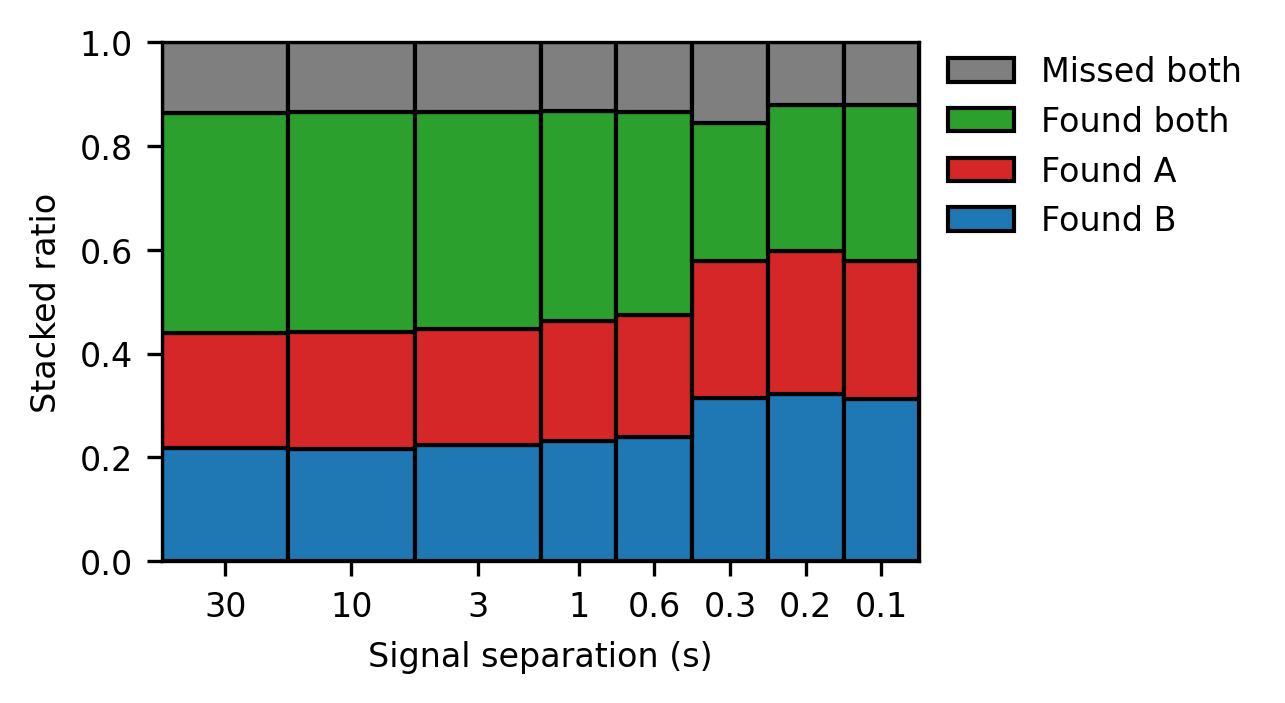
\includegraphics[
	height=6cm, 
	trim=0 0 3cm 0,
	clip]{multiple_signal_detection/plots/detr_stacked}
	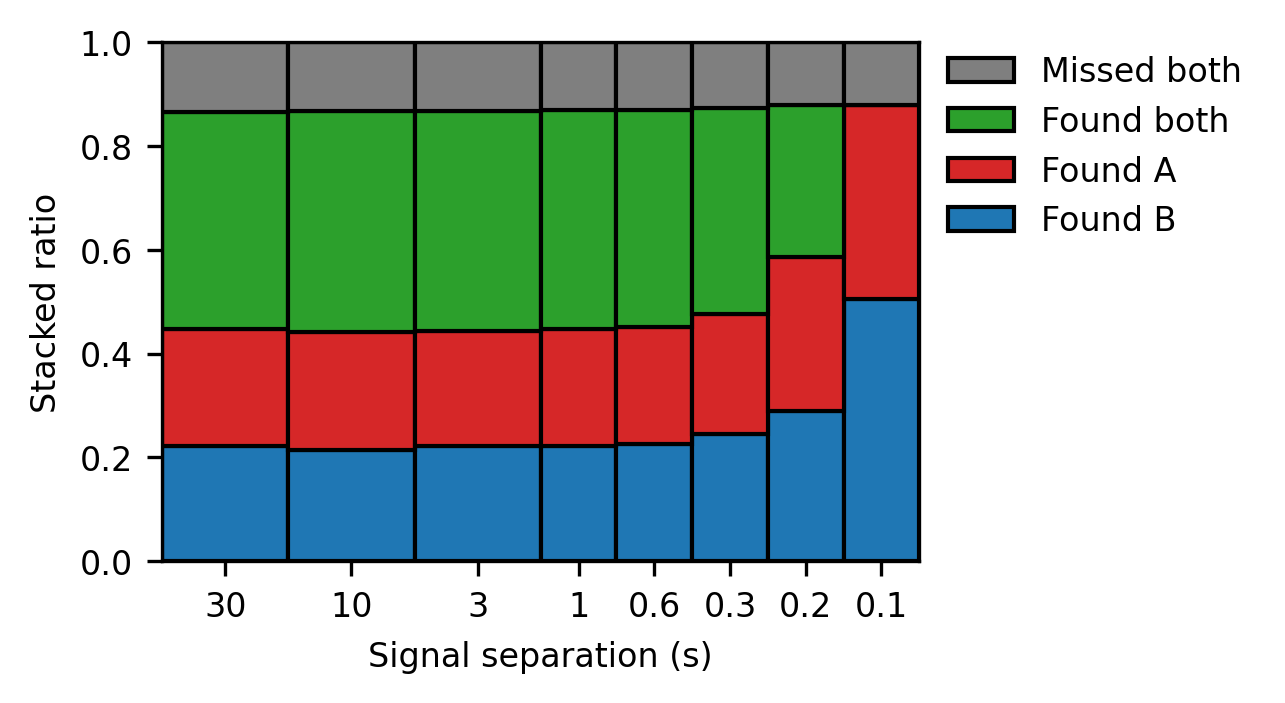
\includegraphics[
	height=6cm, 
	trim=1.3cm 0 0 0,
	clip]{multiple_signal_detection/plots/encoder_stacked}
	}
	\caption{Performance with signal separation for DETR (\emph{left}) and for the heatmap regressor (\emph{right}).}
	\label{fig:detr:deltat_cases}
\end{figure}

\begin{figure}
	\centering
	\makebox[\textwidth]{
		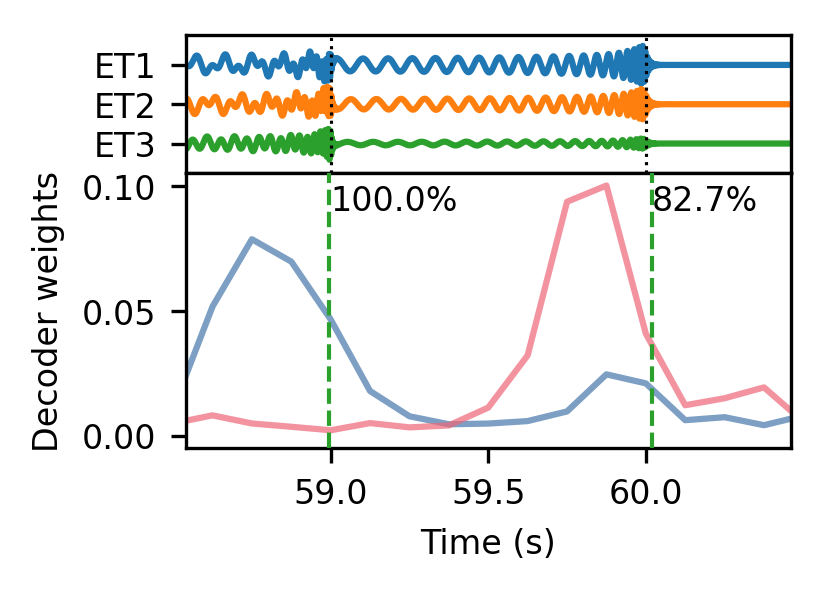
\includegraphics[
		height=5cm,
		trim=0 0 0 0,
		clip
		]{multiple_signal_detection/plots/out/700/detr/0_zoom}
		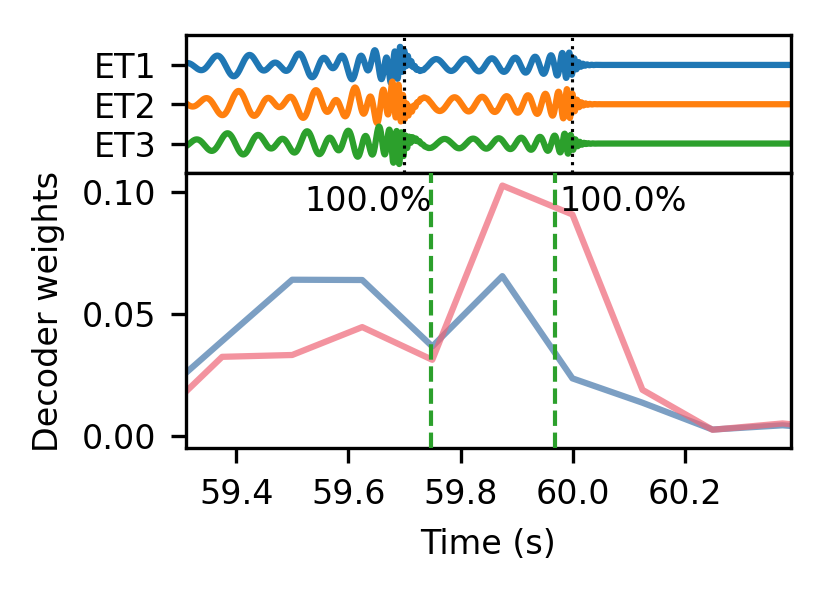
\includegraphics[
		height=5cm,
		trim=1.35cm 0 0 0,
		clip
		]{multiple_signal_detection/plots/out/800/detr/7_zoom}
		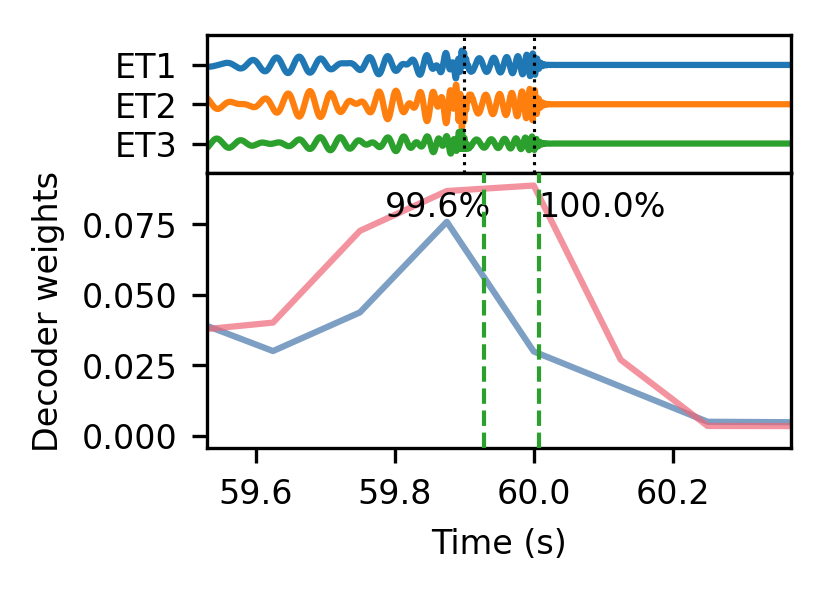
\includegraphics[
		height=5cm,
		trim=1.5cm 0 0 0,
		clip
		]{multiple_signal_detection/plots/out/900/detr/6_zoom}
	}
	\caption{Three example DETR outputs for $\Delta t_\text{coa}=\SI{1}{\second}$ (\emph{left}), $\Delta t_\text{coa}=\SI{0.3}{\second}$ (\emph{middle}) and $\Delta t_\text{coa}=\SI{0.1}{\second}$ (\emph{right}).}
	\label{fig:detr:deltat_plot}
\end{figure}

\section{Discussion}

% DETR performs comparably well
% removes intrinsic bottleneck of heatmap resolution
% easily adapted to produce parameter estimates as well
% direct time prediction yields better results (in a way this is promising for parameter estimation)

DETR demonstrates performance comparable to the heatmap transformer while eliminating its intrinsic bottleneck, the heatmap time-resolution. By directly predicting coalescence times, DETR achieves improved time-accuracy. DETR is easily adapted to predict additional signal parameters in future work.

% Performance still degrades in the edge cases of low fars and close signal separations
% may be attributed to the larger model size and insufficient training (refer to learning curves)

Despite these advantages, the model exhibits reduced performance for low FARs and moderately separated signals with $\SI{1}{\second}\geq\Delta t_\text{coa}\geq\SI{0.3}{\second}$. 
In the regime $\Delta t_\text{coa}\leq\SI{0.2}{\second}$, performance is comparable to or exceeds that of the heatmap regressor, as DETR is free to predict GW candidates regardless of signal separation.

One possible explanation is that these limitations arise from insufficient model optimization rather than architectural flaws. DETR comprises \SI{6.2}{\mega\nothing} trainable parameters compared to roughly \SI{2.2}{\mega\nothing} for the heatmap transformer, while being trained on the same \SI{1}{\mega\nothing} sample dataset. The learning curves (Figs.~\ref{fig:detr:learning_curve} and \ref{fig:detr:tandem}) show that DETR continues improving until epoch $93$, considerably later than the heatmap transformer, which overfit at the 16th epoch. This behavior suggests that additional training and larger datasets might further improve performance.

% future: maybe finetune on the same matching that is used for evaluation instead of hungarian (which is less robust for low fars and clos separations)

Another potential direction is to better align the matching algorithm DETR uses for training (Hungarian matching) with the one employed for evaluation (greedy matching). It can be argued that greedy matching is more robust in low-FAR operating regimes, where DETR has shown worse performance compared to heatmap regression. This is because at low FARs, greedy matching neglects all predictions with scores $\lesssim\SI{100}{\percent}$ and assigns only the highest-score predictions. In contrast, Hungarian matching considers \emph{all} predictions for assignment by minimization of some cost function instead. 
In future work, a one-to-one matching algorithm that is more robust at low FARs like greedy matching could be used for fine-tuning DETR for improved performance in this operating regime.

\chapter{Conclusion}
\label{sec:conclusion}
% models can process 64s long inputs
% transformer based architecture have proven benificial for prediction multiple signals
% in particular, two archtitectures show promising results: transformer heatmap regressor, detr
% both retrieve a non-zero fraction of signals at low FARs of 1/month, while achieving low latencies
% while heatmap performs slightly better at these low FARs, DETR removes post-processing, better time resolution, *can* detect signals regardless of separation, and is easily adapted to parameter estimation

This thesis successfully developed machine-learning models that can detect long-duration, overlapping signals in synthetic ET data. 
This work focuses on black-hole CBCs and uses \SI{64}{\second} long samples. Each sample contains up to six signals, motivated by the expected event rate of \SI{E+5}{\per\year} to \SI{E+6}{\per\year} \cite{abac2025scienceeinsteintelescope}. For one sample, the models output multiple GW candidates, each with a confidence measure and the signal coalescence-time.

In particular, two architectures have been implemented, both showing promising results. These consist of a CNN backbone, as well as transformer components with global attention. 
A CNN backbone efficiently processes the large input to a more condensed latent representation. The backbone treats each ET detector stream as a different channel and employs heavy downsampling afterwards. Using transformer components, the models can efficiently process the whole latent representation. Exploiting \emph{global} information across the whole time series has shown increased performance for detecting multiple, overlapping signals per sample, compared to models with a \emph{local} receptive field.

The two models differ mostly in their output. One is a transformer heatmap regressor, which outputs a \enquote{probability time series}. From this, GW candidates are extracted via peak extraction. The other model is the Detection Transformer (DETR) and outputs candidate events directly.

Both models can retrieve a non-zero fraction of signals at low FARs of $1/\SI{}{\month}$, allowing them to make adequately confident detections for low-latency searches. 
Exact detection ratios are not reported in this conclusion, as these are dataset-dependent, especially on the chosen SNR range, which was not chosen to be realistic here. The results should be understood as proof-of-concept.

These machine-learning algorithms are generally far more computationally efficient than matched filtering. Although not tested, it is reasonable to assume that the models here can process one sample in $<\SI{64}{\second}$, making them compatible with low-latency searches.

Although both models' performance is roughly comparable, and the heatmap regressor even achieves higher detection ratios for low FARs of $1/\SI{}{\month}$, DETR appears more promising as a basis for future work. In particular, DETR\dots
\begin{itemize}[noitemsep,topsep=0pt]
	\item Removes the need for post-processing steps to construct GW candidates.
	\item Makes more accurate time predictions with a standard deviation of \SI{17}{\milli\second} compared to \SI{34}{\milli\second}. 
	\item Can be easily adapted to predict other signal parameters  as well. This is important for low-latency searches. Its improved time-prediction accuracy by direct prediction is promising in this case.
	\item Can make predictions regardless of signal separation. This is not the case for the heatmap regressor and for standard matched filtering searches \cite{Relton_2022}, which only retrieve one of two signals if separations are small.
	\item Might improve with more data and longer training, as suggested by the learning curves.
\end{itemize}

% outlook: detr more data longer training
% try parameter estimation as well
% rework matching algorithm
% work with real detector stream and evaluate on data with realistic snr dist and poissonian number of mergers

Future work should focus on training DETR with more data for more epochs. For increased performance at low FARs, fine-tuning with a reworked	 Hungarian matching scheme could be investigated. DETR is easily adapted to predict signal parameters as well. This should be studied, focusing on the intrinsic parameters such as the masses and spins first.

Finally, models need to be evaluated on more realistic ET-like data. This includes the simulation of a proper detector stream, which is split into \SI{64}{\second} samples later. These will contain the inspiral parts of signals with coalescence times outside the sample window. Further, instead of sampling the number of signals uniformly, these should follow a Poissonian distribution with the expected ET event rate. Instead of sampling the SNRs uniformly, signals should be simulated ensuring some distance distribution. Usually, this is a second-order power law.

\printbibliography

\appendix
\chapter{Quadrupole Moment}
\label{app:quadrupole}

\begin{figure}
	\centering
	\makebox[\textwidth]{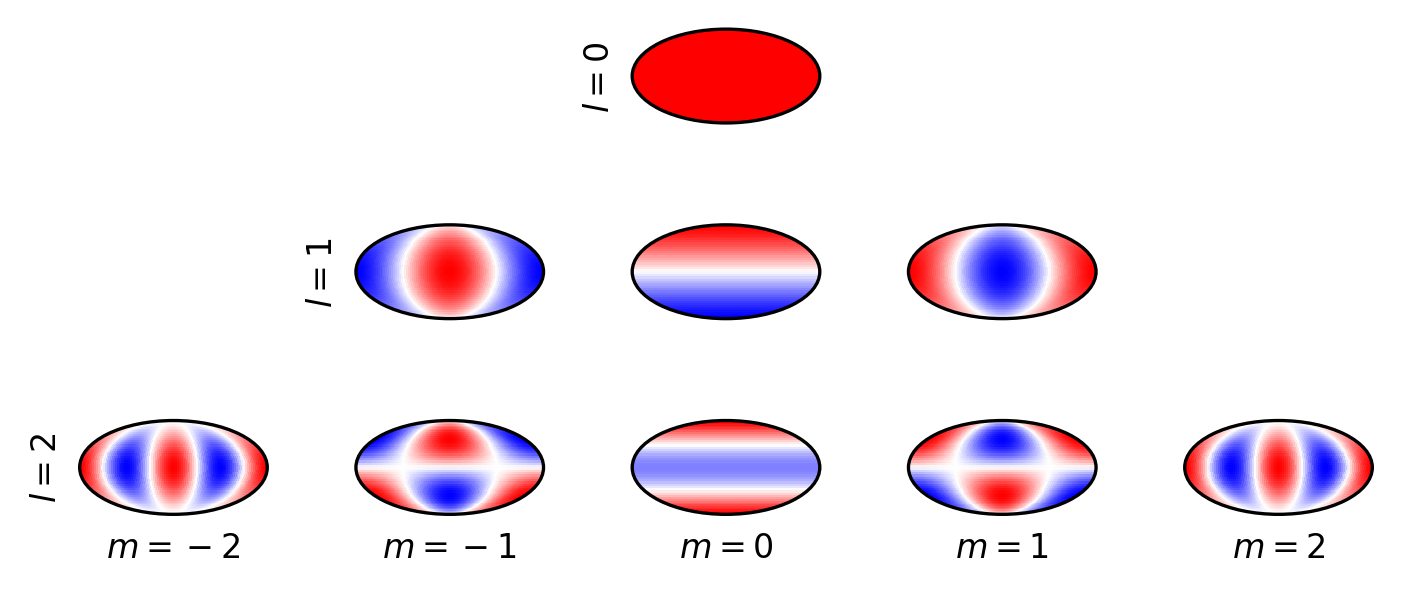
\includegraphics[width=12cm]{theory_of_gravitational_waves/images/spherical_harmonics/spherical_harmonics}}
	\caption{Visualization of the spherical harmonics up to $l=2$. The plots show the normalization of $\Re Y^m_l(\theta,\phi)$ on a Mollweide projection.}
	\label{fig:gravitational_waves:spherical_harmonics}
\end{figure}

In the transverse-traceless gauge, the quadrupole moment tensor takes the form,
\begin{equation}
	Q_{ij} = \int\mathrm{d}^3\vec{r}\,(3r_ir_j - \delta_{ij}r^2)T_{00}(t, \vec{r}).
\end{equation}
By expanding the energy density $T_{00}$ as
\begin{equation}
	T_{00}(t, \vec{r}) = \sum_l \sum_{m=-l}^l \rho_{lm}(t, r)Y^m_l(\theta, \phi)
\end{equation}
with the spherical harmonic functions $Y^m_l$ and coefficients $\rho_{lm}$, it can be shown that only the $l=2$ coefficients contribute to the quadrupole moment tensor.
This follows from the fact that $3r_ir_j - \delta_{ij}r^2$ can be expanded purely in $l=2$ spherical harmonics. That is,
\begin{equation}
	\label{eq:appendix:quadrupole}
	3r_ir_j - \delta_{ij}r^2 = r^2\sum_{m=-2}^{2}c_mY^m_{l=2},
\end{equation}
which will be verified later. Then, 
\begin{equation}
	Q_{ij} = \sum_{m'}\sum_{l,m}\tilde{c}_{m'}
	\int\mathrm{d}r\,r^4\rho_{lm}(t, r)\,
	\int\mathrm{d}\Omega\,
	(Y_{l'=2}^{m'})^* Y_{l}^{m},
\end{equation}
making use of $(Y_l^m)^* = (-1)^mY^{-m}_l$, and defining $\tilde{c}_m = (-1)^{-m}c_{-m}$.
The orthonormality of the spherical harmonics,
\begin{equation}
	\int\mathrm{d}\Omega\,(Y^{m'}_{l'})^*Y^m_l = \delta_{ll'}\delta_{mm'},
\end{equation}
yields
\begin{equation}
	Q_{ij} = \sum_{m}\tilde{c}_m\int\mathrm{d}r\,r^4\rho_{l=2,m}(t, r).
\end{equation}
This shows that the quadrupole moment tensor is non-vanishing only if the mass distribution has a non-zero $l=2$ spherical harmonic contribution. From this it is obvious that spherically symmetric ($l=0$) systems do not radiate. See Fig.~\ref{fig:gravitational_waves:spherical_harmonics} for a visualization of the spherical harmonics. The $l=2$ distributions are peanut-shaped. Prime examples of time-varying systems with $l=2$ mass distributions are orbiting binary systems.

Eq.~\ref{eq:appendix:quadrupole} can be written out explicitly as, 
% chat gpt says to put 3 instead of 2 for 3x²-r² and 3y²-r²
\begin{align}
	3x^2 - r^2 &= 3\sqrt\frac{2\pi}{15}r^2(Y^2_2+Y^{-2}_2) - 2\sqrt\frac{\pi}{5}r^2Y^0_2, \\
	3y^2 - r^2 &= -3\sqrt\frac{2\pi}{15}r^2(Y^2_2+Y^{-2}_2) - 2\sqrt\frac{\pi}{5}r^2Y^0_2, \\
	3z^2 - r^2 &= 4\sqrt\frac{\pi}{5}r^2Y^0_2, \\
	xy &= -i\sqrt{\frac{2\pi}{15}}r^2(Y^2_2-Y^{-2}_2), \\
	yz &= i\sqrt{\frac{2\pi}{15}}r^2(Y_2^1+Y_2^{-1}), \\
	zx &= -\sqrt\frac{2\pi}{15}r^2(Y_2^1 - Y_2^{-1}).
\end{align}
This can be verified from the $l=2$ harmonics:
\begin{alignat}{2}
	Y_{2}^{-2}(\theta,\varphi)
	& = \frac{1}{4}\sqrt\frac{15}{2\pi}\e^{-2i\varphi}\sin^{2}\theta
	&& = \frac{1}{4}\sqrt\frac{15}{2\pi}\frac{(x - iy)^2}{r^{2}}, \\
	Y_{2}^{-1}(\theta,\varphi)
	& = \frac{1}{2}\sqrt\frac{15}{2\pi}\e^{-i\varphi}\sin\theta\cos\theta
	&& = \frac{1}{2}\sqrt\frac{15}{2\pi}\frac{(x - iy)z}{r^{2}}, \\
	Y_{2}^{ 0}(\theta,\varphi)
	& = \frac{1}{4}\sqrt\frac{5}{\pi}(3\cos^{2}\theta-1)
	&& = \frac{1}{4}\sqrt\frac{5}{\pi}{(3z^{2}-r^{2})\over r^{2}}, \\
	Y_{2}^{ 1}(\theta,\varphi)
	& = -\frac{1}{2}\sqrt\frac{15}{2\pi}\e^{  i\varphi}\sin\theta\cos\theta
	&& = -\frac{1}{2}\sqrt\frac{15}{2\pi}\frac{(x + iy) z}{r^{2}}, \\
	Y_{2}^{ 2}(\theta,\varphi)
	& = \frac{1}{4}\sqrt\frac{15}{2\pi}\e^{ 2i\varphi}\sin^{2}\theta
	&& = \frac{1}{4}\sqrt\frac{15}{2\pi}\frac{(x + iy)^2}{r^{2}}.
\end{alignat}


\end{document}